%----------------------------------------------------------------------------------------
%	PACKAGES AND OTHER DOCUMENT CONFIGURATIONS
%----------------------------------------------------------------------------------------

\documentclass[12pt]{article} % Default font size is 12pt, it can be changed here

\usepackage{geometry} % Required to change the page size to A4
\usepackage{graphicx} % Required for including pictures
\usepackage{float} % Allows putting an [H] in \begin{figure} to specify the exact location of the figure
\usepackage{hyperref} % Enables hyperlinks and text reference clicking
\usepackage{color} % Enables text font coloring
\usepackage{caption} 
\usepackage{subcaption} 
\usepackage{fancyhdr} % adds headers and footers
\usepackage{indentfirst} % Indents the first paragraph in a section
\hypersetup{
    colorlinks,
    citecolor=black,
    filecolor=black,
    linkcolor=blue,
    urlcolor=blue
}

\definecolor{orange}{rgb}{1,.5,0}
\definecolor{darkgreen}{rgb}{0,.66,0}
\definecolor{lightblue}{rgb}{0,1,1}
\definecolor{pink}{rgb}{1,.46,.75}
\definecolor{beige}{rgb}{.97,.83,.75}
\pagestyle{fancy}
\lhead{Project 2 Group 1 (tjones21 \& razeitz \& special)}
\rhead{\hyperlink{MyToc}{\small{jump to: }Table of Contents}}
\cfoot{}
\lfoot{\thepage}
\rfoot{\today}

% \renewcommand{\headrulewidth}{0.4pt}
% \renewcommand{\footrulewidth}{0.4pt}
\newcommand{\HRule}{\rule{\linewidth}{0.5mm}} % Defines a new command for the horizontal lines, change thickness here
\renewcommand{\contentsname}{Project Content Navigation (\textcolor{blue}{clickable})}
\graphicspath{{img/}} % Specifies the directory where pictures are stored

% \geometry{a4paper} % Set the page size to be A4 as opposed to the default US Letter
%\usepackage{lipsum} % Used for inserting dummy 'Lorem ipsum' text into the template
%\usepackage{wrapfig} % Allows in-line images such as the example fish picture
%\setlength\parindent{0pt} % Uncomment to remove all indentation from paragraphs

\begin{document}

\begin{titlepage}

  \center % Center everything on the page

  \textsc{\LARGE Usability Engineering}\\[1.5mm] 
  \textsc{\Large CS/ISE 5714 - Spring 14}\\[1mm] 
  \textsc{Project 2: Contextual inquiry and contextual analysis}\\[1mm] 
  %In this project assignment you perform contextual inquiry and analysis, starting with a field visit to understand the existing customer, client, or user work (or play) practice, the activities people undertake to accomplish goals in the work or play domain and the complete work context.

  % the deliverable states'One-line description of this project assignment'
  % I think the name of the 'product' and its general purpose is good a description of the deliverable
  { \small Inkhorn: a scheduling and feedback system enhance tailored coaching services to patrons }\\
  \HRule
  \vspace{4mm}

  \begin{minipage}{0.4\textwidth}
  \begin{flushleft} \small
  \emph{TEAM 1:}\\
  T.C. \textsc{Jones} \href{mailto:tjones21@vt.edu}{tjones21@vt.edu}\\
  Rebecca \textsc{Zeitz} \href{mailto:razeitz@vt.edu}{razeitz@vt.edu}\\
  Chris \textsc{Frisina}  \href{mailto:special@vt.edu}{special@vt.edu}\\
  \end{flushleft}
  \end{minipage}
  ~
  \begin{minipage}{0.4\textwidth}
  \begin{flushright} \small
  \emph{Client:} \\
  The Writing Center\\
  Jennifer \textsc{Lawrence}  \href{mailto:jlwrnc@vt.edu}{jlwrnc@vt.edu}
  %Assistant Director of the Writing Center\\
  \end{flushright}
  \end{minipage}\\
  [5mm]
  
  \begingroup
  \def\addvspace#1{}
    \tableofcontents\hypertarget{toc}{}
  \endgroup
\end{titlepage}

\newpage
% TODO Not sure if we should match all sections to number since we dont have all sections and some overlap
\section{System Concept Statement} %1
% To make this report a stand-alone document, repeat the latest version of your system concept statement, as a synopsis of your project. UPDATE it addressing the comments from Project 1. Include just the concept statement, not the full project 1. 

  % What is the system name?  
  % –Who are the system users?  
  % –What will the system do? 
  % –What problem(s) will the system solve? (Be broad to include business objectives)
  % What is design vision and what are the emotional impact goals?
  % what experience will system provide to user
  % Audience broader than that of most other deliverables, including   
  % – High-level management 
  % – Marketing 
  % – Board of directors  
  % – Stockholders  
  % – Even general public

  % I dont think we should start of with the product without noting who is involved and the base for a problem -CHRIS
  Inkhorn will serve the Writing Center by providing a common ground tool for use among coaches and other staff.
  It will allow users, the Writing Center staff, to match coaches with patrons requesting a session by providing a more systematic, but still personalized, scheduling process.
  % I dont know what this means -CHRIS
  As a feedback system, Inkhorn will allow for patron privacy not currently available.
  % good -CHRIS
  Furthermore, Inkhorn will serve as a tool for coaches to suggest resources and methods that will coincide with the needs and goals of the patrons.
  Inkhorn will help tailor writing enhancing coaching services to specific patrons’ needs, such as with conference or course papers, technical documents, personal statements, or other interpersonal communications.
  % I dont think this is what we are offering, as this is an entirely different scope.  Now they converse on IH as well? -CHRIS
  Playing off the informal but professional atmosphere of the Writing Center, Inkhorn will be a space for users to converse and share thoughts and ideas.
  % i am not sure a bridge is the best description we can come up with -CHRIS
  In essence, Inkhorn will act as a bridge between the coaches, administrative staff, and patrons.

  --

  The Virginia New River Valley community members often seek support services surrounding improving their communication skills and understanding of the English language.
  The Virginia Tech Writing Center (WC) provides varying personal coaching services for locals in addition to VT affiliates.
  To maintain the personal touch the WC exemplifies, we propose Inkhorn, an automated scheduling and feedback system, will help tailor coaching services to patrons to develop their skills to enhance their writing, such as conference or class papers, personal statements, and interpersonal communications. 
  % Speak directly towards the emotional impact -CHRIS
  To increase a positive milieu between coach and patron, Inkhorn will help manage recommendations from the coach that coincide with the needs of the patron, as well as streamline and retain coach feedback from the patron.
  Inkhorn will also help promote services offered by WC, manage session scheduling with compatible coaches, automate reporting, provide a continual coach feedback system, manage forms, and suggest appropriate tools for patrons' goals.

\section{Tailor The Scope} %2
% Describe how you made decisions to tailor the scope of this assignment for your own project and give justification where appropriate
  Among our initial ideas for clients and problems, we focused on writing.
  % we should probably just say writings, since non technical and sotries is also 'repetitive', although this isn't a point of contention for me given it isn't my strongest domain-CHRIS
  Our initial problem was in the realm of collaborative writing techniques for technical, novel, and story telling writers.
  Given client scheduling problems, we had to abandon this idea.
  % the client is both the wc and JL, I dont think it is needed to specify JL - CHRIS
  Our next client in the writing domain we chose was the Virginia Tech Writing Center (WC), and the Assistant Director Jennifer Lawrence.
  % I think the years enhances our assessment of her knowledge - CHRIS
  She has served in this role for 7 years, and her extensive knowledge alongside positional status makes her the ideal candidate within the WC to initially contact and get organizational information, as well as follow communication for project details.

\section{Preparation for Interview} %3
% Describe the process of preparation for interviewing and observation in your contextual inquiry. 
  Preparation for interviews and observation of the Writing Center (WC) included background research on the Writing Center.
  We scoped out the WC web pages, taking note of the goals, processes, and other information that was present.
  Doing this, and gathering initial, informal accounts of patrons who have used the WC, enabled the team to get a feel for the presence the WC holds within the VT community.
  The websites and initial perspectives from previous patrons of the writing center helped us gather initial insight into the culture of the work domain and the surrounding impact of the WC.
  The initial impression of the WC we formulated was that the WC services a wide range of subjects or academic fields, all tied to the process of writing.
  Furthermore, we gathered that the writing center uses a phone call scheduling system for creating appointments and accepts walk-ins.
  This told us that the WC uses a person-based, as well as a mix of formal and informal scheduling system. 

  The writing commonality, being fore fronted, was further specified through our initial findings that the WC helps with papers, essays, resumes, cover letters, and personal writings.
  From the websites, we also got an initial feel for the population of WC patrons, those being not only VT affiliates, but the Blacksburg community as well.
  This was noted by the WC additional location at the Montgomery-Floyd Regional Library.
  In terms of the WC staff population, we could tell from the websites that the upper level management team consists of VT English department faculty and the coaches hired can be VT students from any majors who have meet the application process requirements. 

  One of our team members contacted the WC to inquire about the WC staff and determine who would be a fitting interviewee.
  Once we did our background investigation, we decided to interview the assistant director, Jennifer Lawrence, and one of the WC coaches.
  We drafted and revised interview questions based on their work roles and other aspects of the WC and the writing domain.

\section{Who Was Interviewed} %4
% How many client representatives and/or users did you interview in total and how did you decide that? List their names, job titles, responsibilities, and anything else that would help describe their role in the enterprise.
  Excluding our previous client, we interviewed two people, encompassing three distinct roles (one person has two roles).
  Our initial phone conversation with the WC hinted that the Assistant Director Jennifer Lawrence was the best initial contact person for the majority of the assignment concerns.
  Reviewing the website also helped ascertain the majority of the services provided by the WC.
  She also works as a coach, which was known from the initial email that she replied to about meeting for an interview.
  A brainstorming session with group members allowed us to iterate over questions that would provide information to complete the assignment, as well as provide a structured interview style that would also serve as a positive first introduction.
  We noticed that some questions were best addressed to specific roles, so we separated the questions accordingly for Jennifer, and used the `Coach' questions for Nneoma Enyi Nwankwo, another coach whose schedule aligned and agreed to interview in person with a recording.
  We plan to continue to interview other coaches who have different skills, in addition to the remaining people who are involved in the information flow related to the services provided by the WC.

\section{Interview Questions} %5
% Include a copy here of the initial questions you prepared for the interviews. 
  \begin{tabbing}
  Assistant Director
  \end{tabbing}
  \begin{enumerate} \itemsep1pt \parskip0pt \parsep0pt
  	\item How long have you served as a writing director?
  	\item Who is your supervisor?
  	\item Are there any requirements you have to do as a VT affiliated service?
  	\item How would you describe the atmosphere of the Writing Center?
  	\item What services does the writing center provide?
  	\item What policies exist?
  	\item Are their any current initiatives being offered or planned at TWC
  	\item How long does a coach typically work at TWC 
  	\item What compensation do coaches receive?
  	\item What types of questions and writings do writers bring in? (see website for what student can bring in)
  	\item In a session, how are the WC coaches expected to get their thoughts and comments across to the writer? {on paper, orally, etc.}
  	\item Is there any record keeping?
  	\item Is there a feedback, rating system, or complaint system?
  	\item What contingency plans are there (for example, what if a coach doesn’t show?  what if a writer doesn’t show?)
  	\item Does coach seniority gain any benefits, tangible or otherwise?
  	\item What auxiliary management tools do you use?
  \end{enumerate}
  \begin{tabbing}
  Coach(es)
  \end{tabbing}
  \begin{enumerate} \itemsep1pt \parskip0pt \parsep0pt
  	\item What year are you in school?
  	\item What is your major or majors?  Any minors?
  	\item Why did you decide to become a Writing Center coach?
  	\item How long have you been working at the Writing Center?
  	\item How long do you plan on working at the Writing Center?
  	\item As a coach, how would you describe the atmosphere of a session?
  	\item Describe the overall process when a writer comes into the WC?
  	\item Are there any other tools you use?
  	\item Are there assigned seating arrangements for the coaches?
  	\item Do writers make multiple appointments to discuss the same work?
  	\item How do you keep track of a writer’s drafts?
  	\item How do you utilize a writer’s past drafts?
  	\item Do you ever have multiple writers come in for help on the same document?
  	\item How does the user take notes?
  	\item Are there any policies that you follow? 
  	\item What policies are outdated?  
  	\item In a session, how do you get your thoughts and comments across to the writer? {on paper, orally, etc.}
  	\item How do you give your ideas and comments (verbally, on paper, etc.)?
  	\item What are some of the harder things to help writers with?
  	\item How/where/who do you get your feedback from?
  	\item Do you feel you get enough feedback? Is it constructive?
  	\item What things do you enjoy about your work here?
  	\item What do you feel your strengths are as a coach?
  	\item Do you know the other coaches?
  	\item Are you happy with your compensation?
  	\item How does working with ESL writers differ from native speakers?
  	\item Do you help with LaTeX?
  	\item Do you write frequently outside of work?  If so, what types of works or genres do you write?
  \end{enumerate}

\section{Meeting Description} %6
% Describe briefly how the meeting went with your initial contacts. 
  The interviews were scheduled ahead of time, and for the appropriate amount of time.
  Coupled with our preparation, the interviews moved at a steady organized pace and we received proper amounts of data and information form the questions we asked, along with domain specific knowledge that could not have been planned for.
  The interviewers were pleased with the initial set of questions, and eager to see what information we will provide them in the coming process.

\section{Data Collection} %7
% Describe how you collected raw contextual data and what kind you collected
  We collected the blank forms that were readily available, and the most recent statistics that were available.
  We received these by asking each person for any documentation that they might have in addition to the ones we were familiar with from the interviews.
  We also crawled the public facing documentation from the website, took pictures of the facility, and made phone calls prior to visiting to gauge processes, people, and atmosphere.

\section{Artifacts} %8
% Show photos or scans of any work artifacts you collected. 
  \begin{figure}[H]
  \centering
  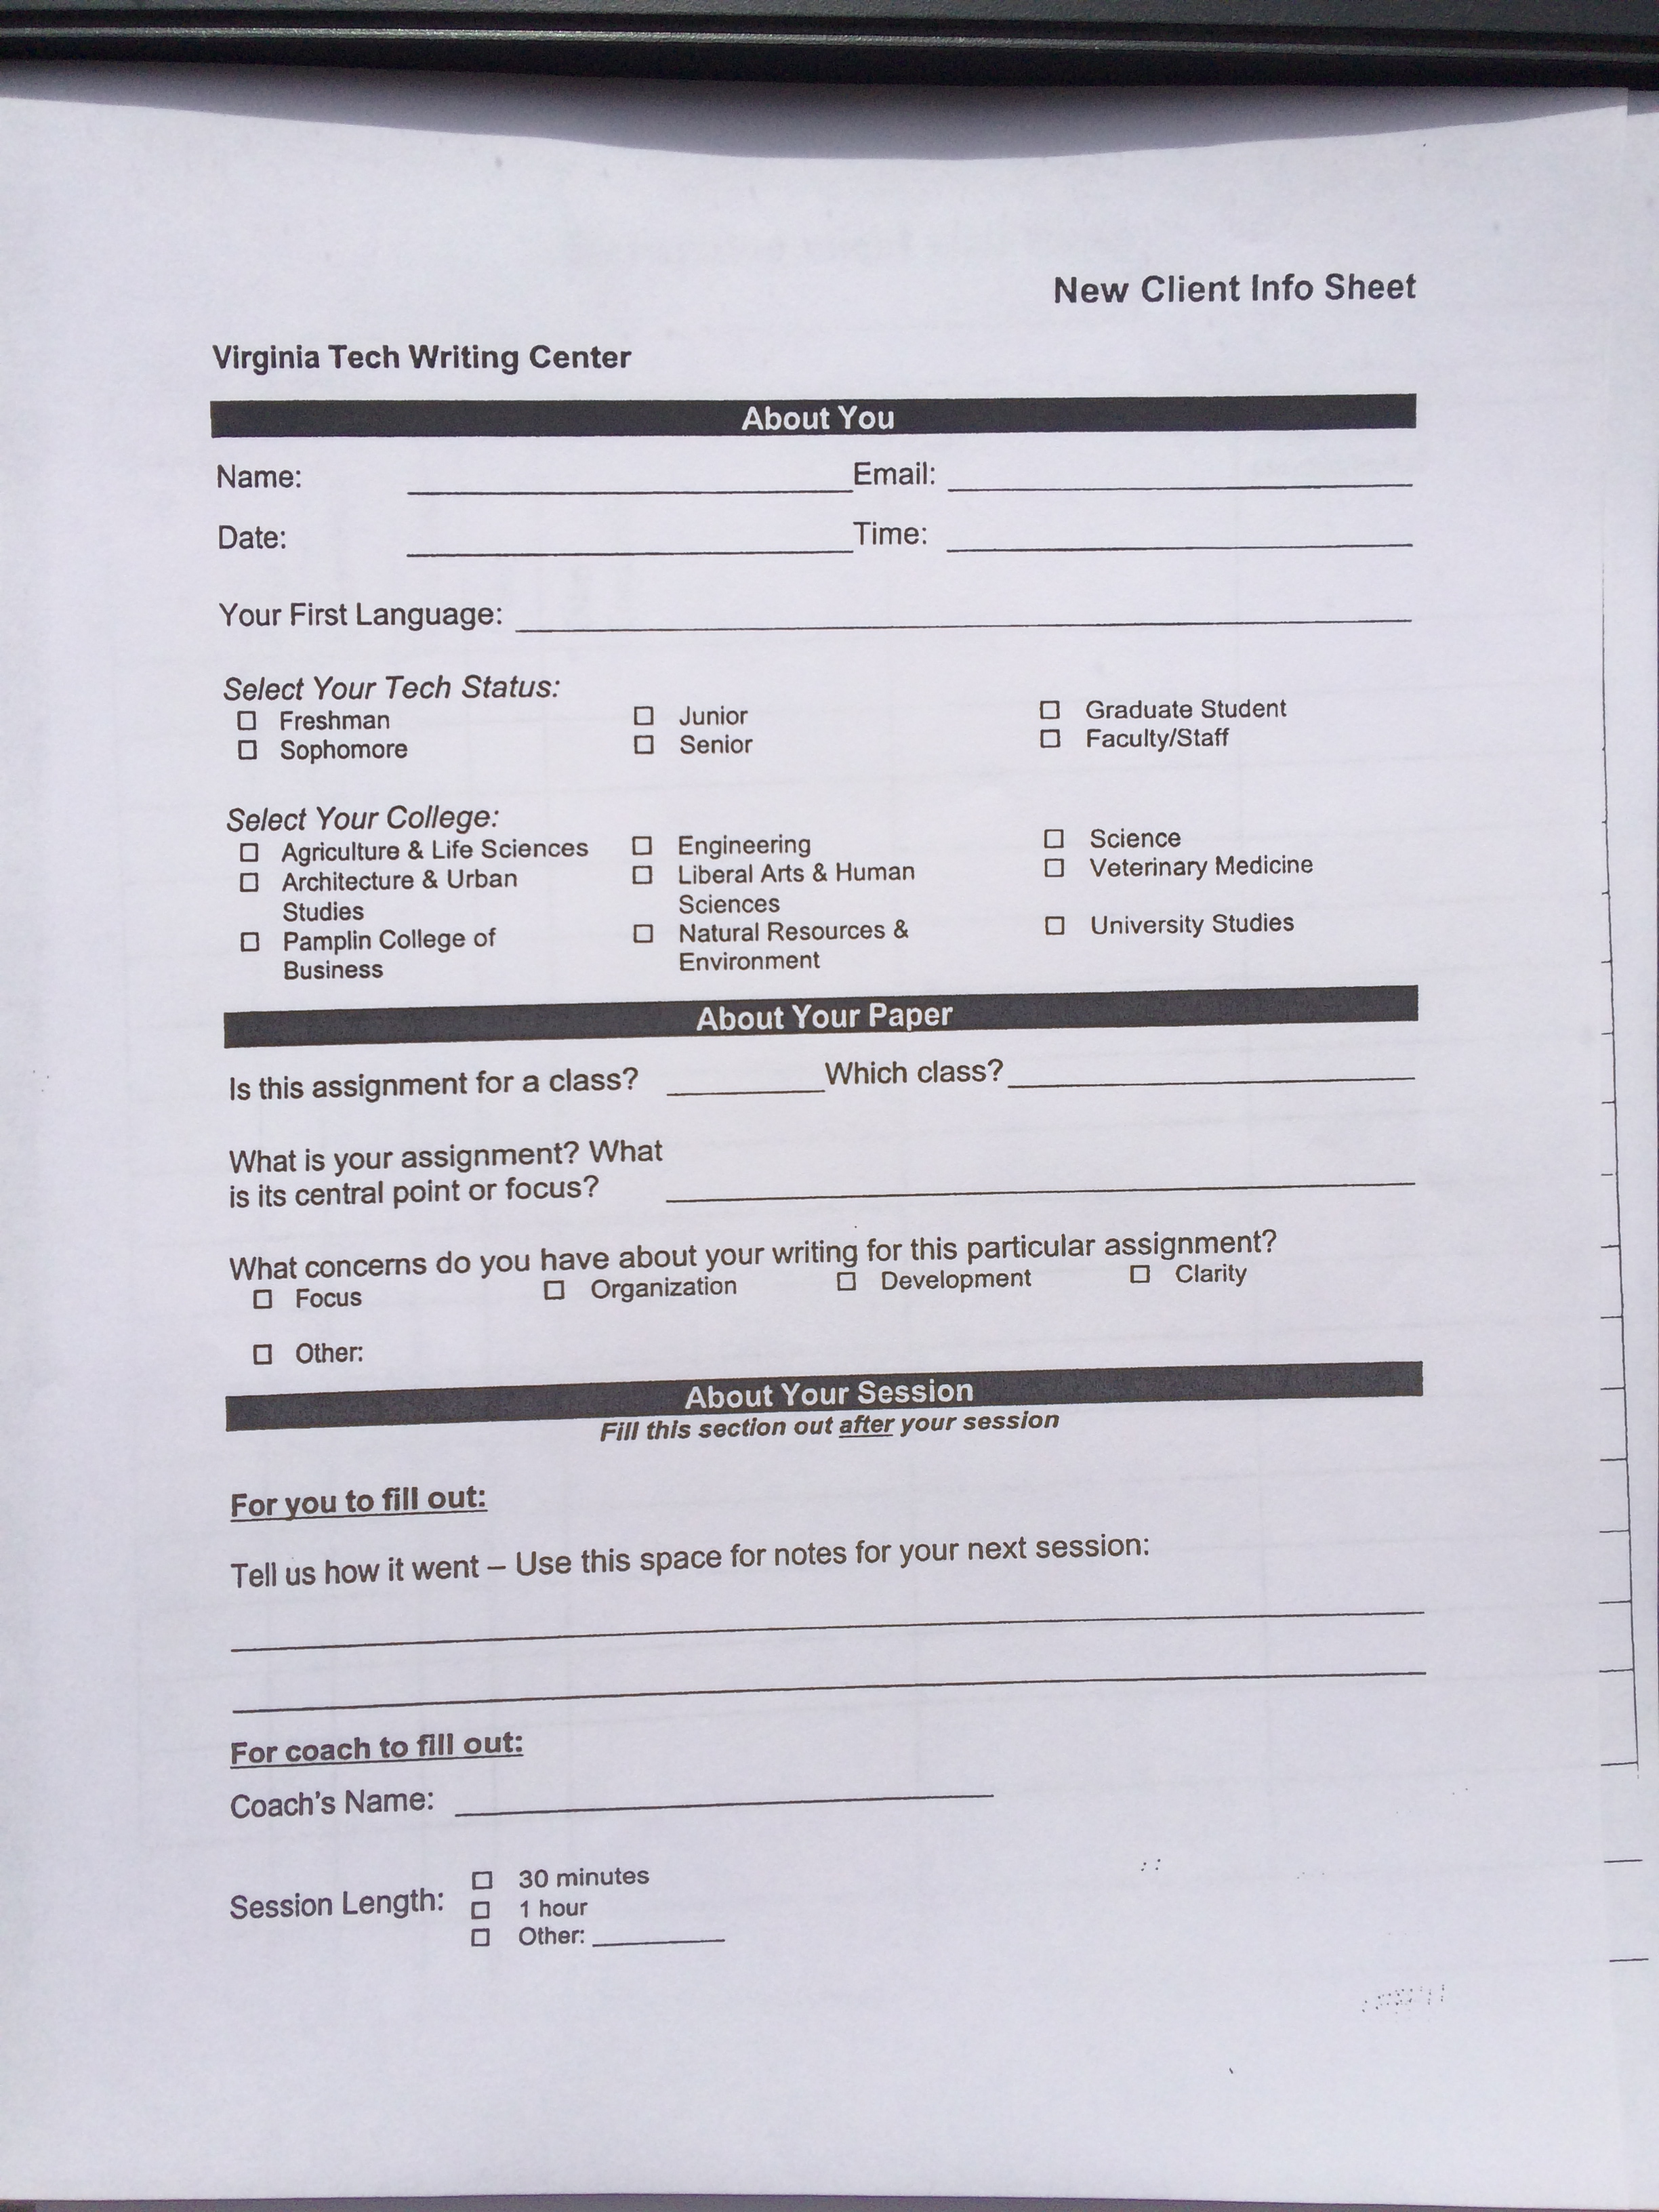
\includegraphics[width=0.5\linewidth]{artifacts/new_client_form}
  \caption{New patron form. Patrons fill this out when they visit the Writing Center for the first time.}
  \label{fig:NewClientForm}
  \end{figure}

  \begin{figure}[H]
  \centering
  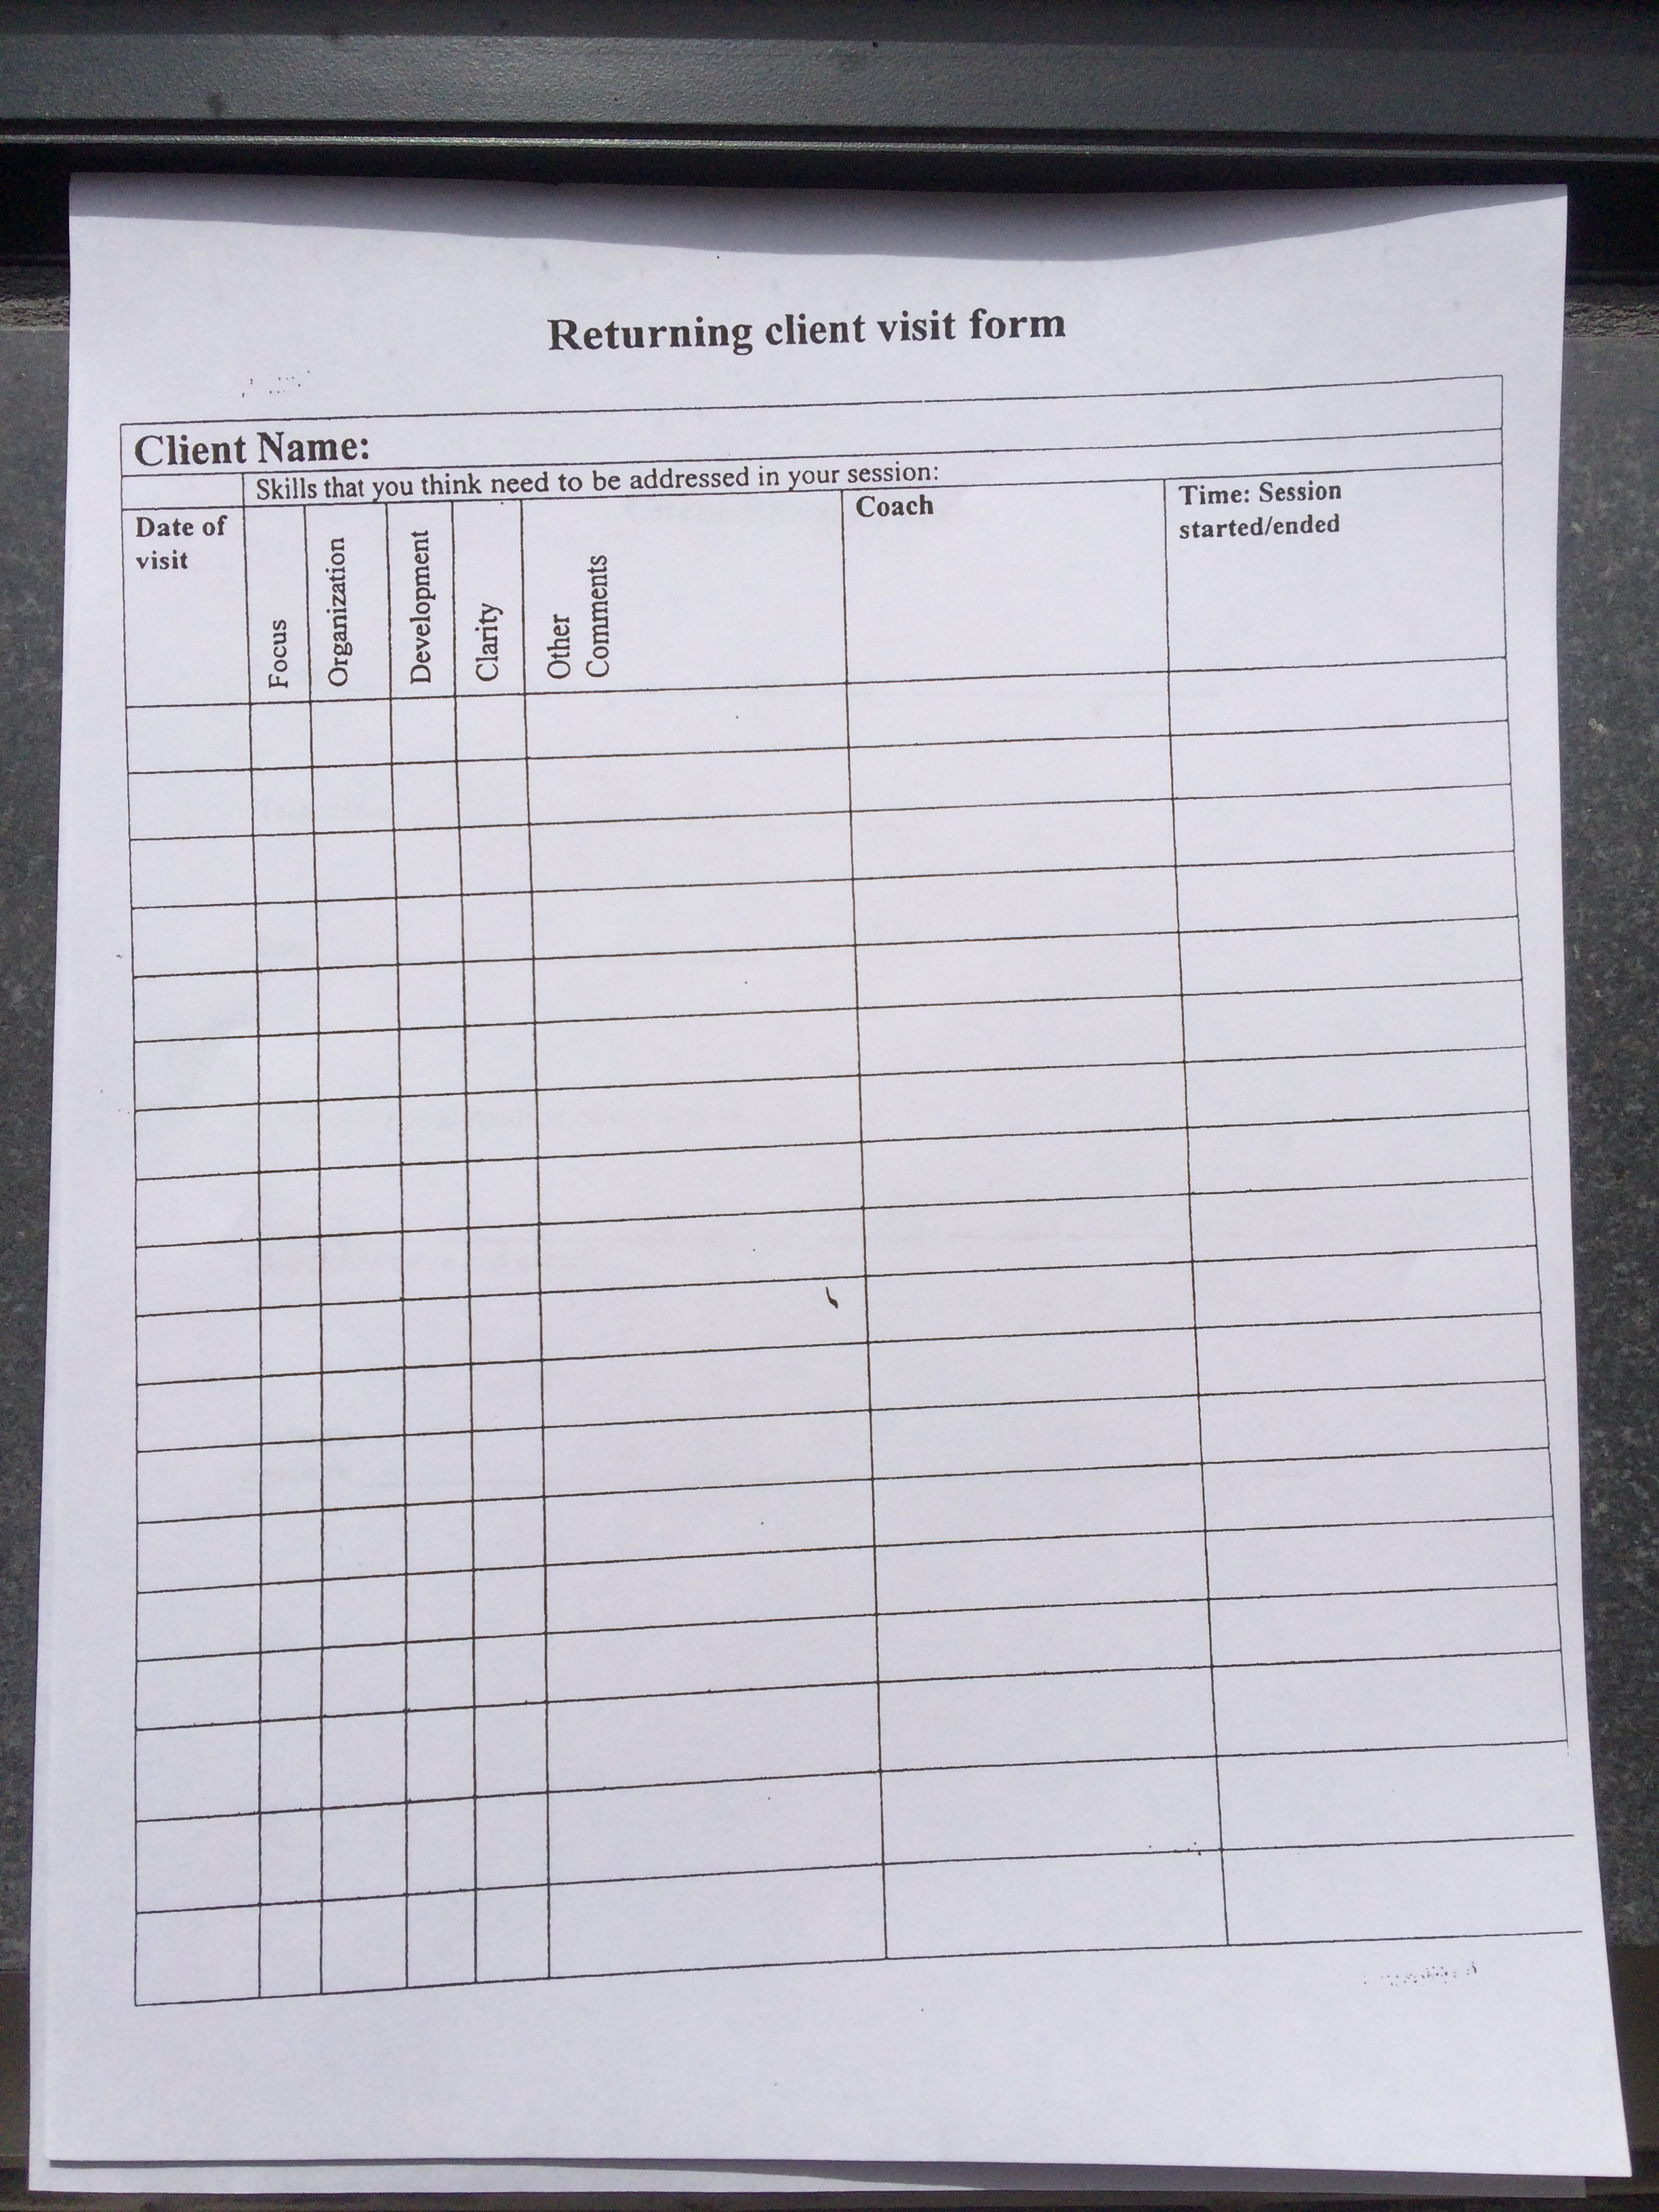
\includegraphics[width=0.5\linewidth]{artifacts/returning_client_form}
  \caption{Returning patron form. Patrons fill this out if they visit the Writing Center more than once.}
  \label{fig:ReturningClienttForm}
  \end{figure}

  \begin{figure}[H]
  \centering
  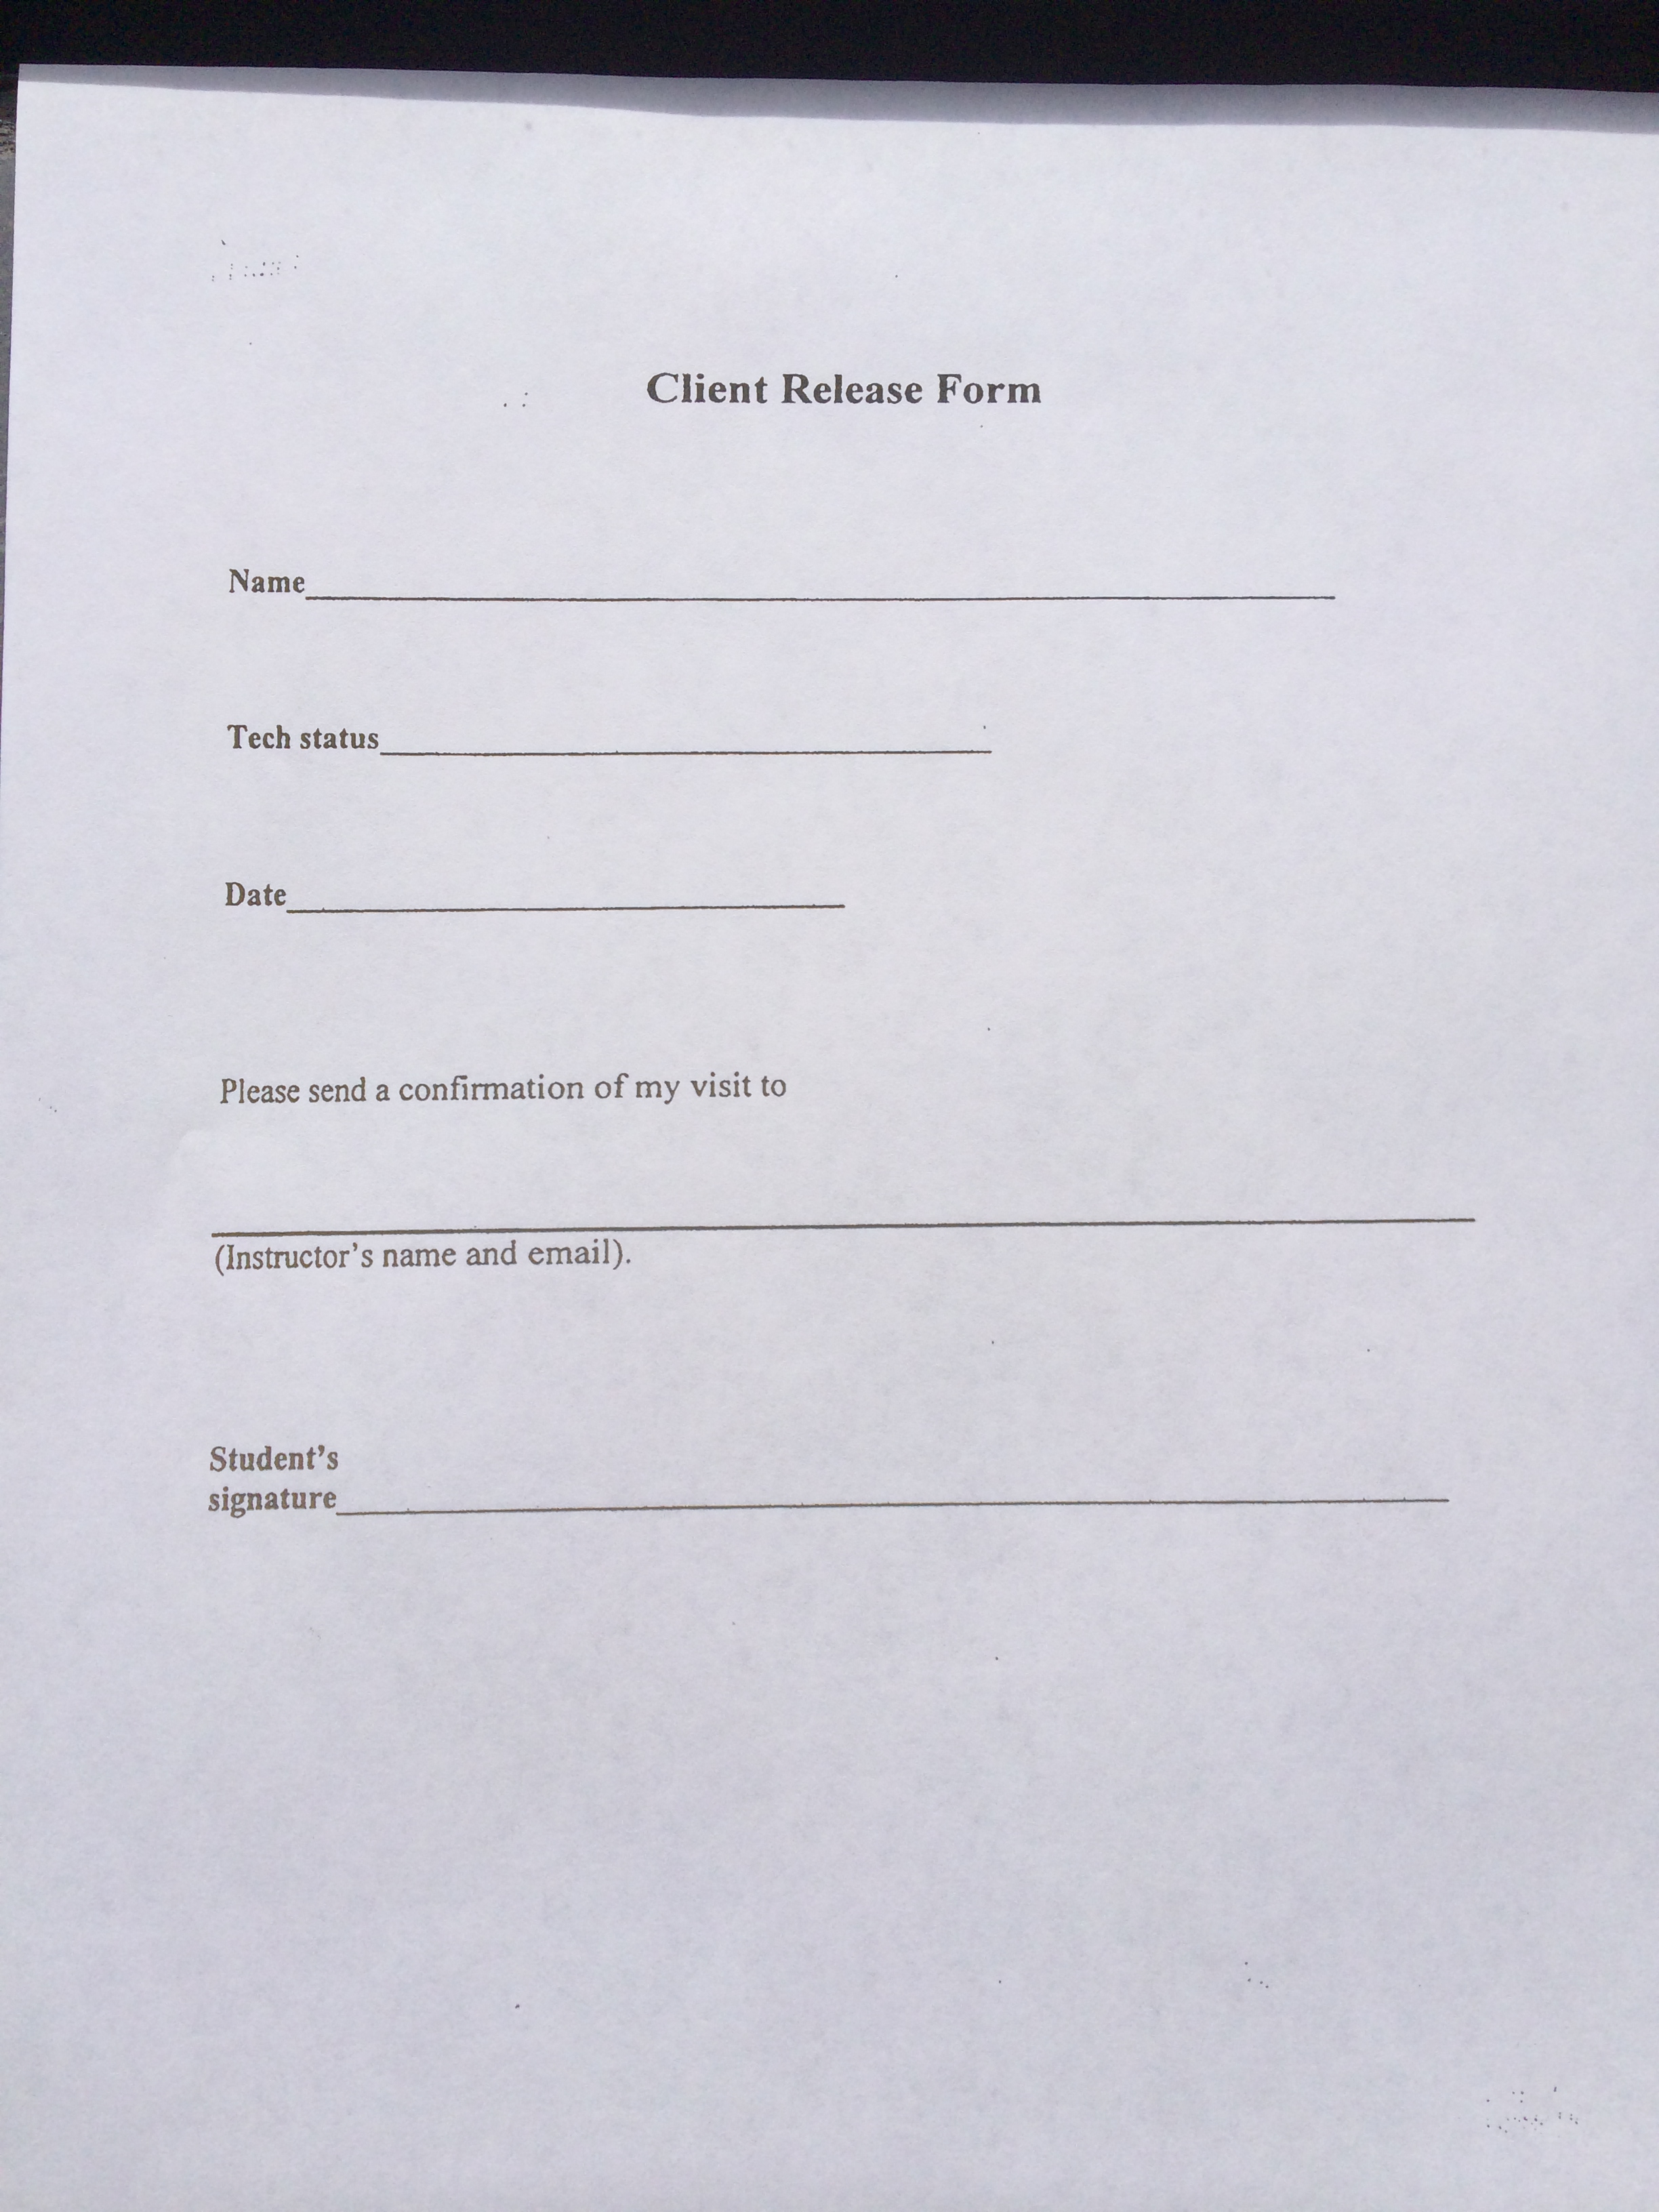
\includegraphics[width=0.5\linewidth]{artifacts/client_release_form}
  \caption{Patron release form.}
  \label{fig:PatronReleaseForm}
  \end{figure}

  \begin{figure}[H]
  \centering
  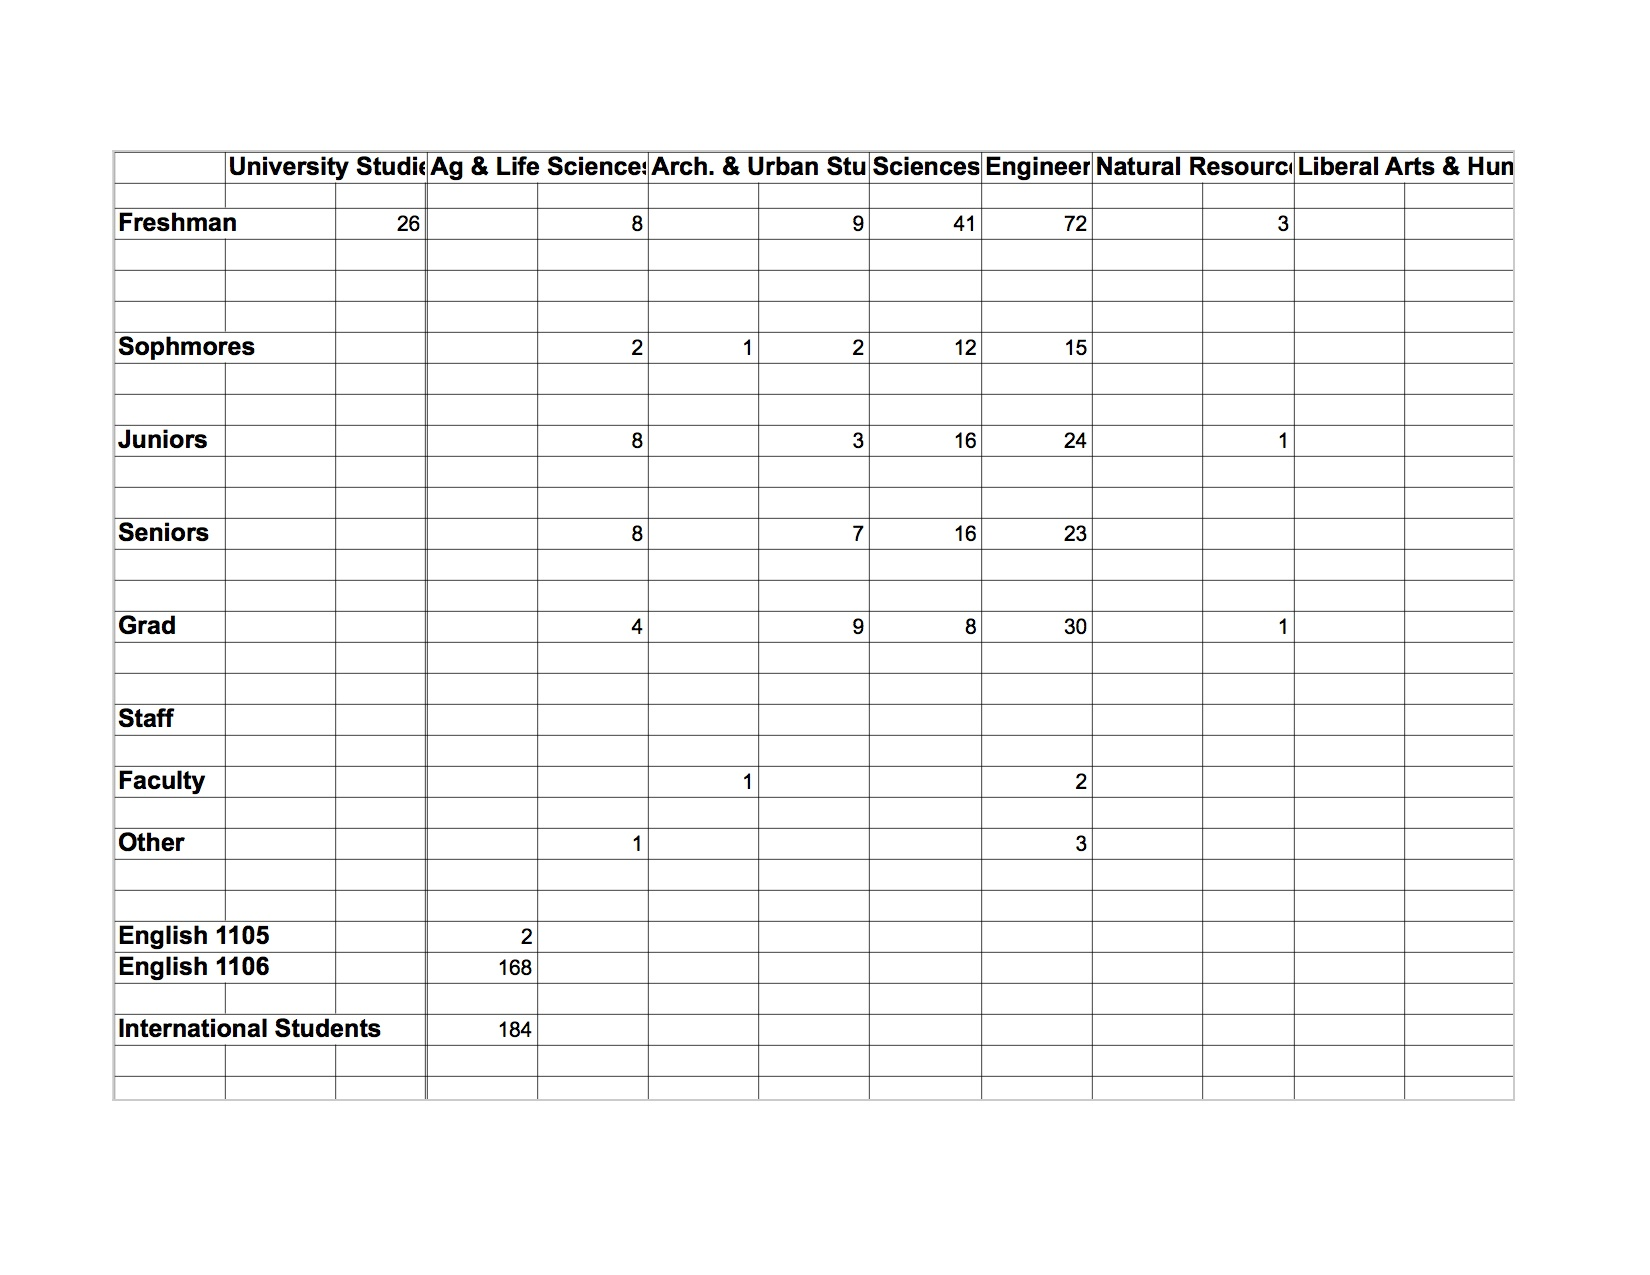
\includegraphics[width=0.5\linewidth]{artifacts/short_term}
  \caption{Short Term (Semester Long) Statistics}
  \label{fig:StatisticsShortTerm}
  \end{figure}

  \begin{figure}[H]
  \centering
  
\includegraphics[width=0.5\linewidth]{artifacts/long_term}
  \caption{Long Term (Several Years) Statistics}
  \label{fig:StatisticsLongTerm}
  \end{figure}

\begin{samepage}
\section{Photos} %9
% Show a representative selection of photos you took. 
  \begin{figure}[H]
  \begin{subfigure}{.5\linewidth}
  \centering
  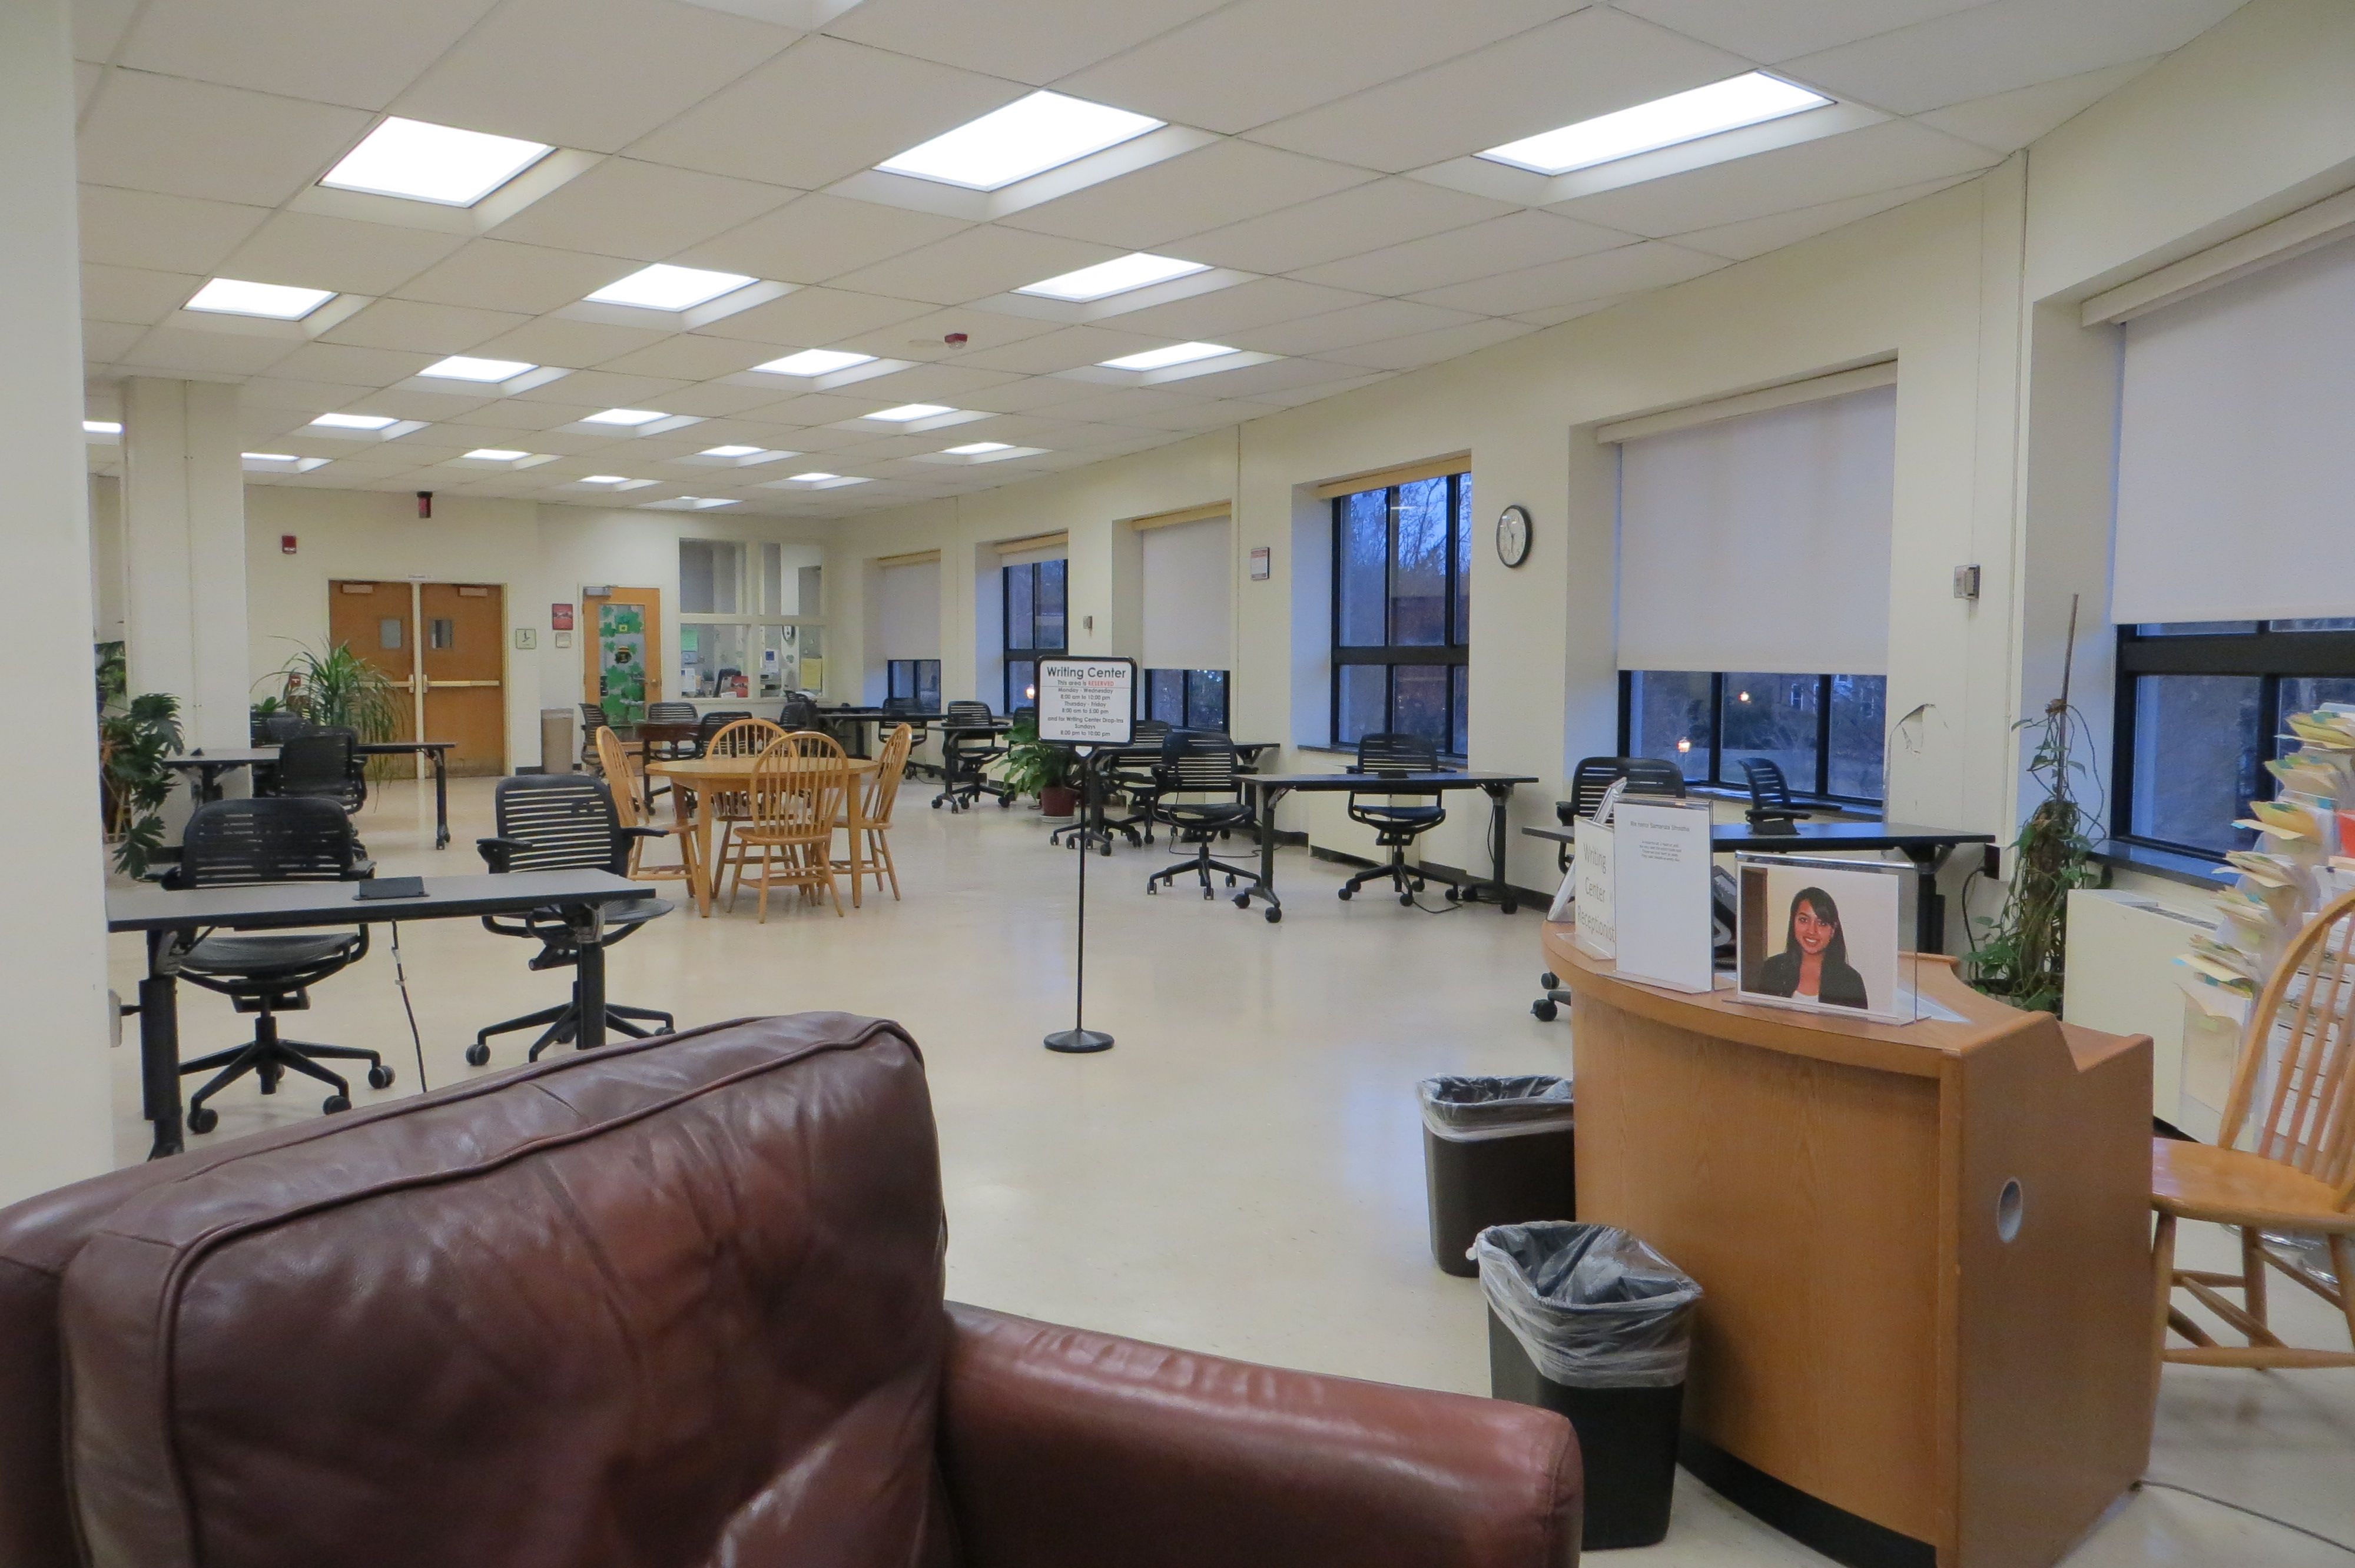
\includegraphics[width=0.75\linewidth]{WC1}
  \caption{}
  \label{fig:WC1}
  \end{subfigure}%
  \begin{subfigure}{.5\linewidth}
  \centering
  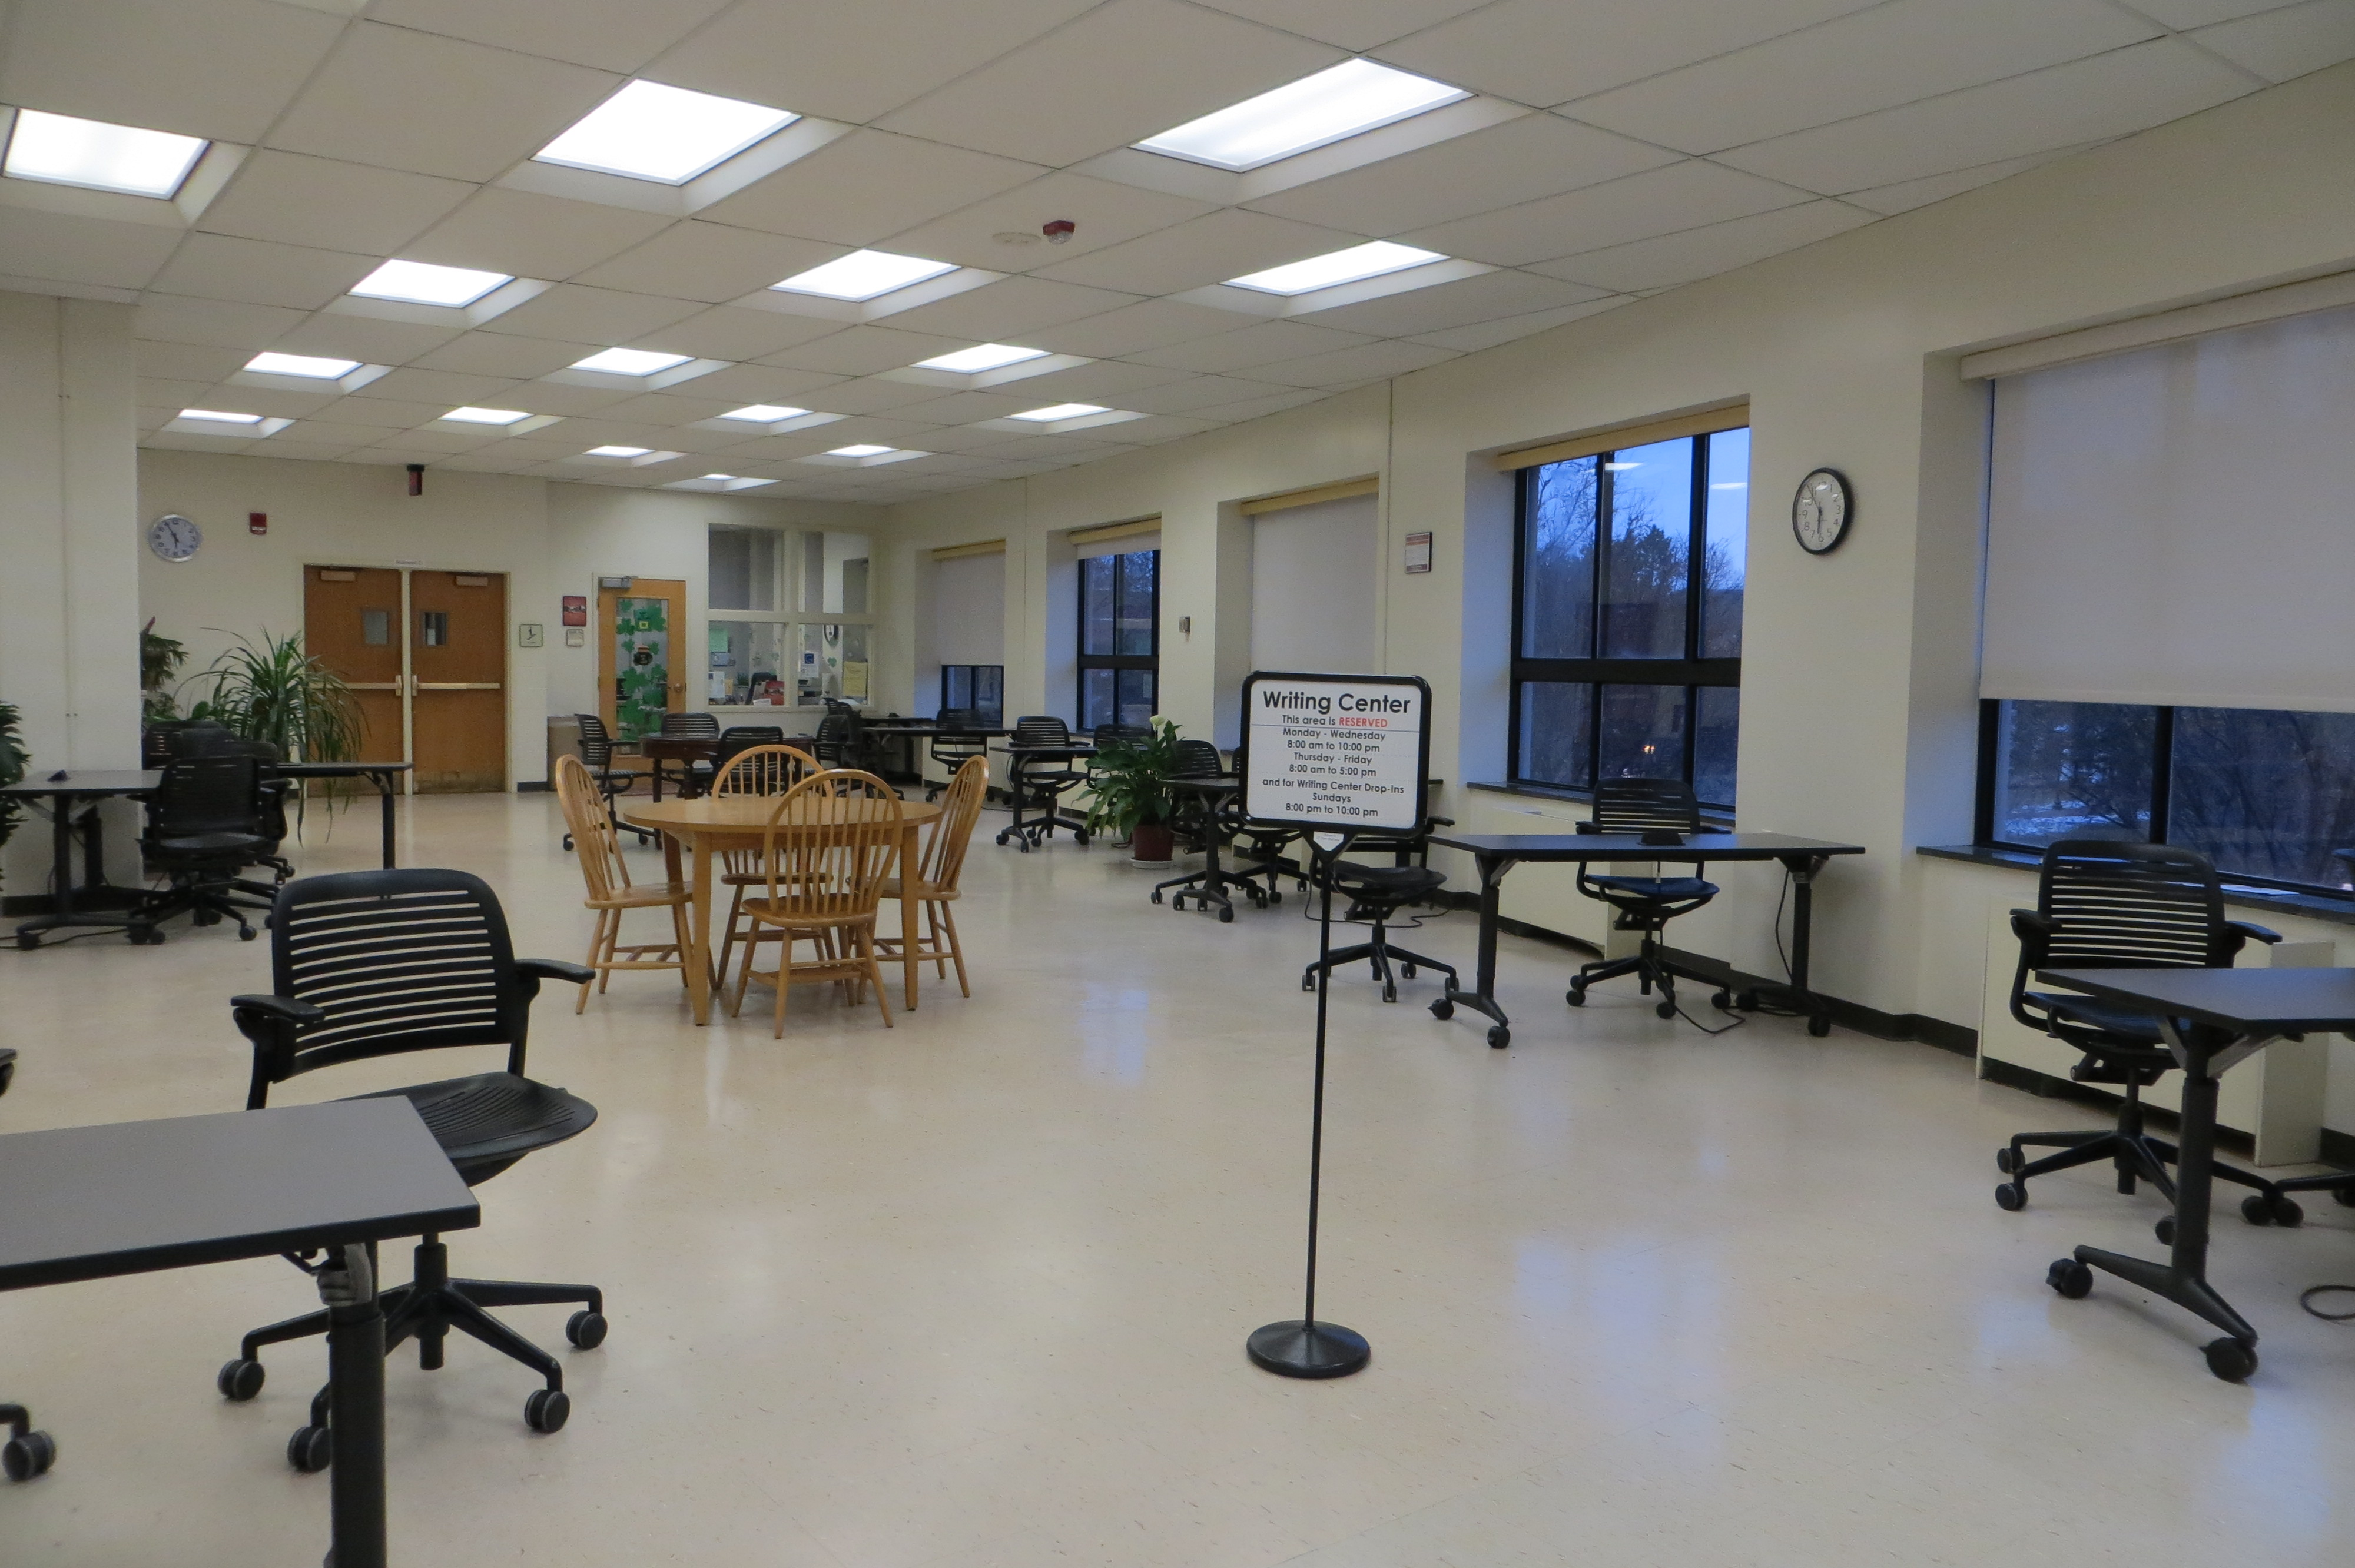
\includegraphics[width=0.75\linewidth]{WC2}
  \caption{}
  \label{fig:WC2}
  \end{subfigure}\\[1ex]
  \begin{subfigure}{.5\linewidth}
  \centering
  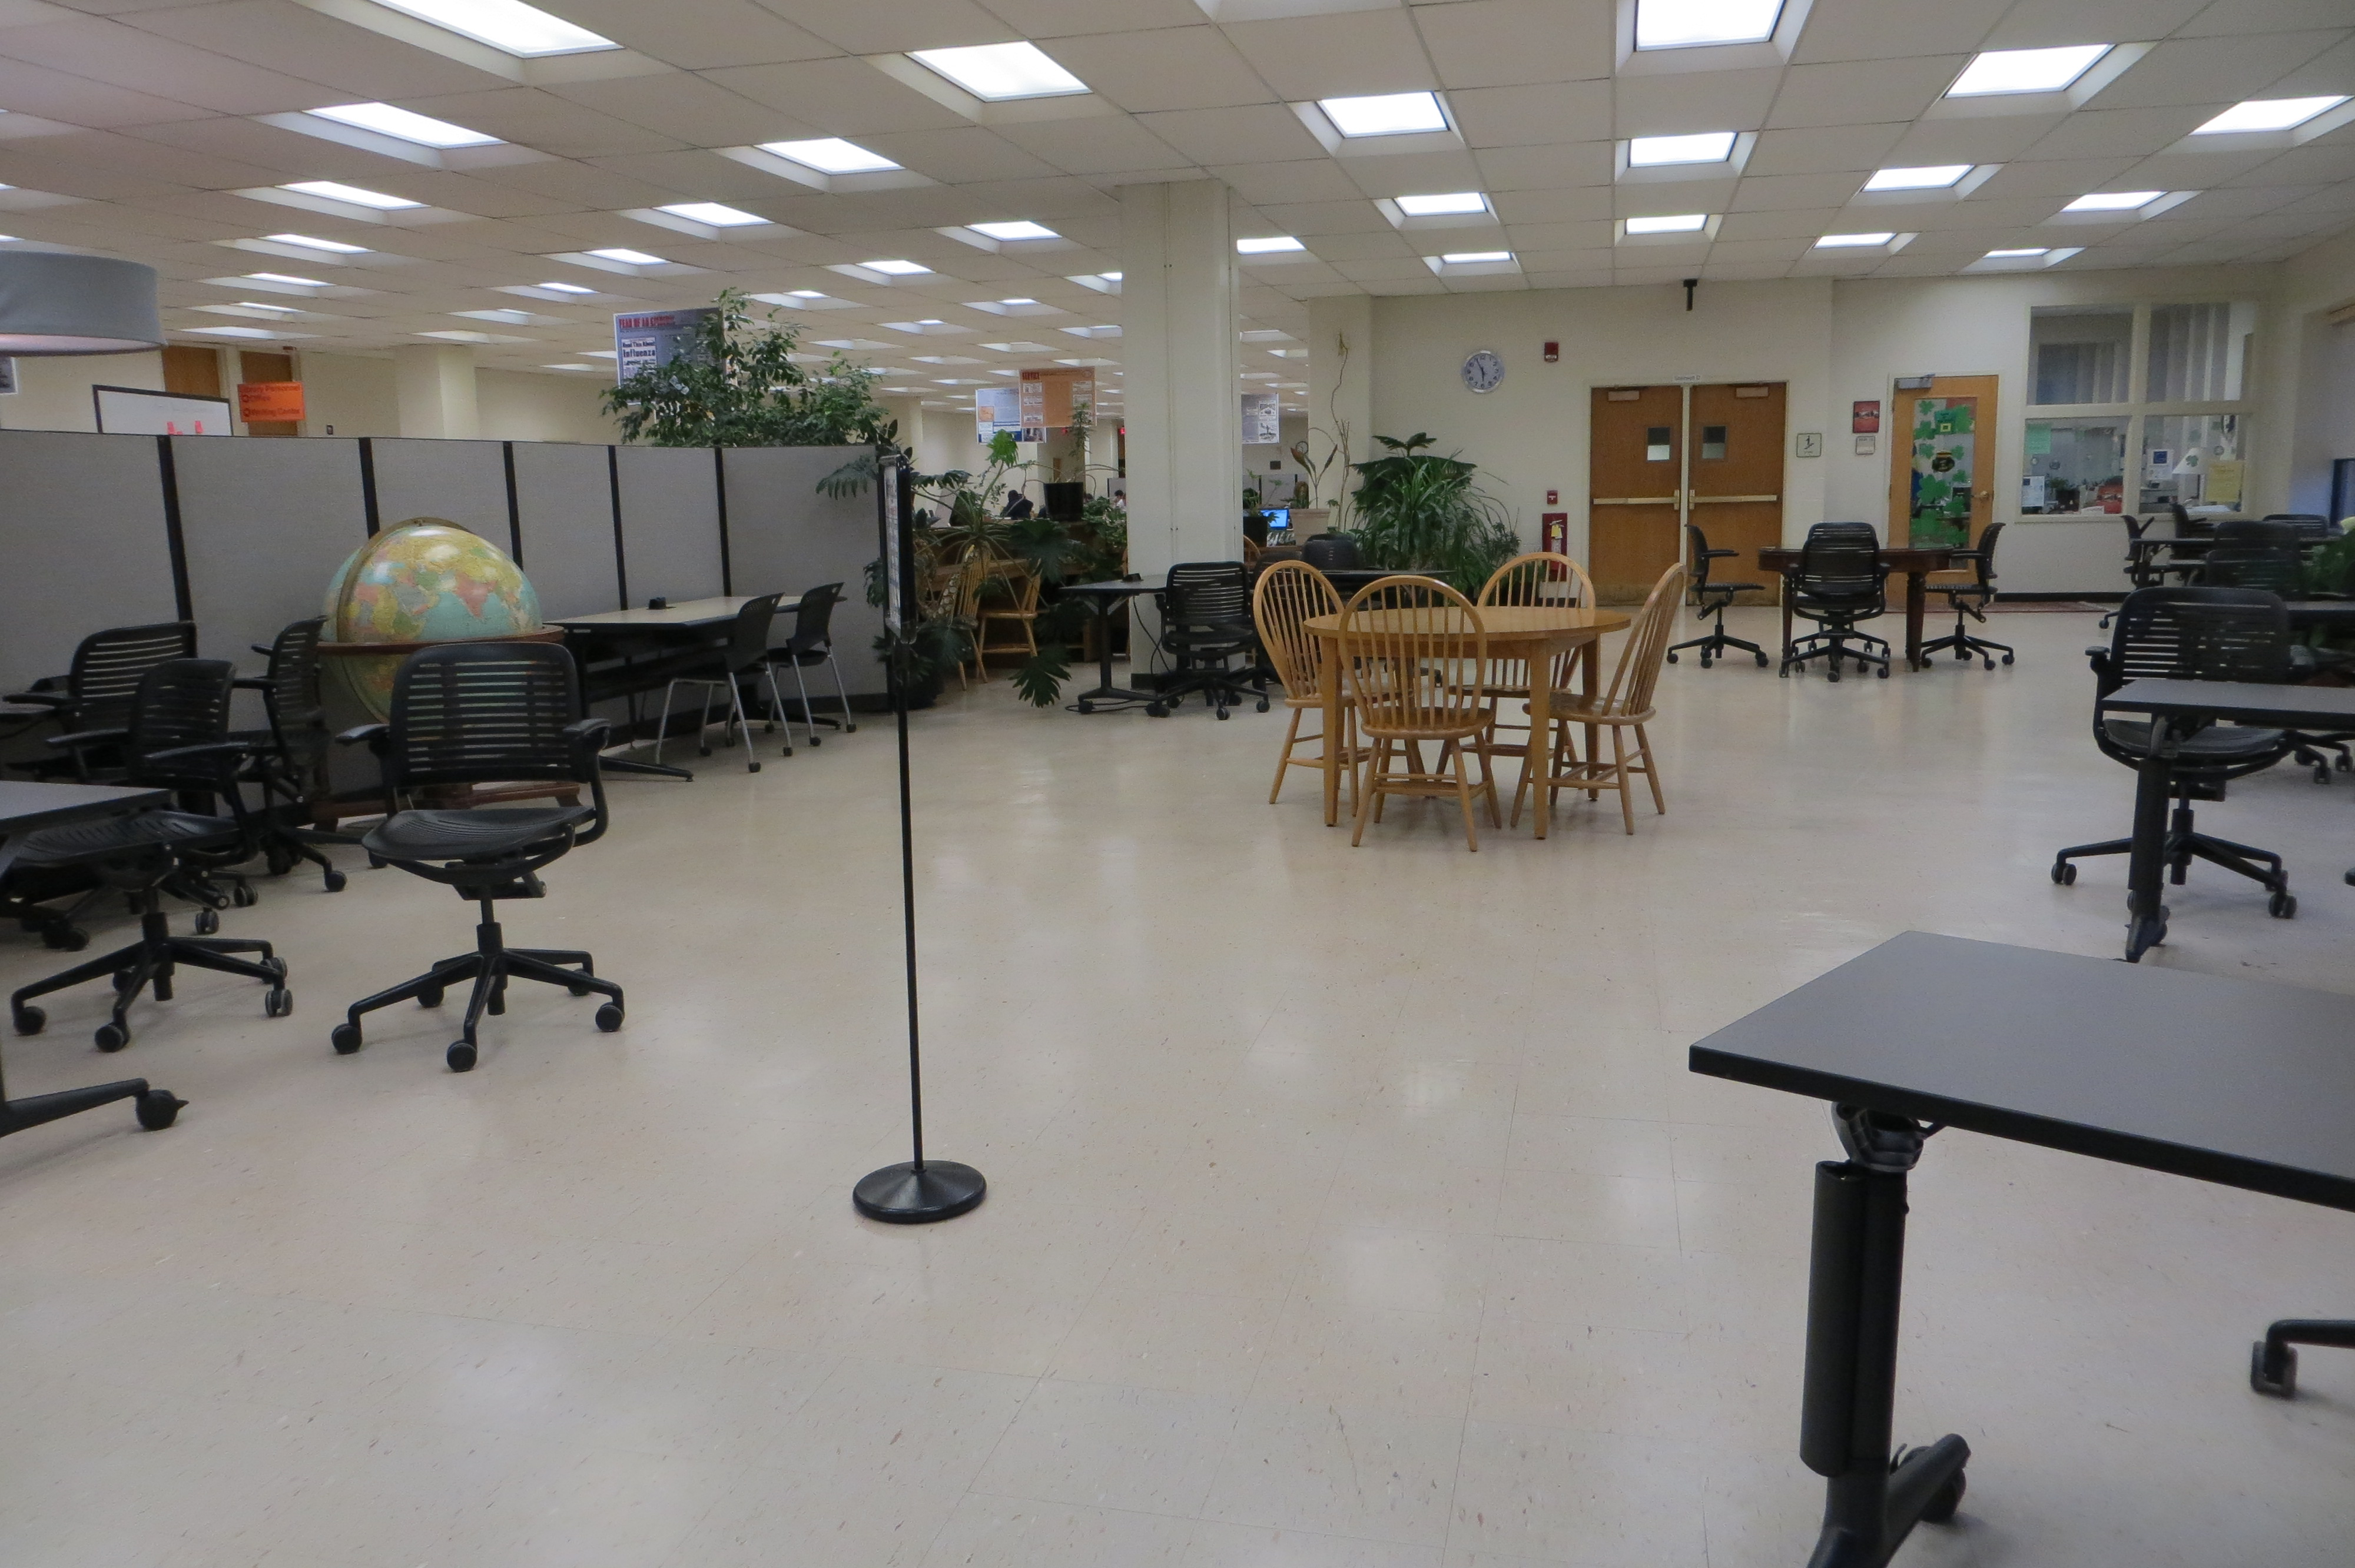
\includegraphics[width=0.75\linewidth]{WC3}
  \caption{}
  \label{fig:WC3}
  \end{subfigure}%
  \begin{subfigure}{.5\linewidth}
  \centering
  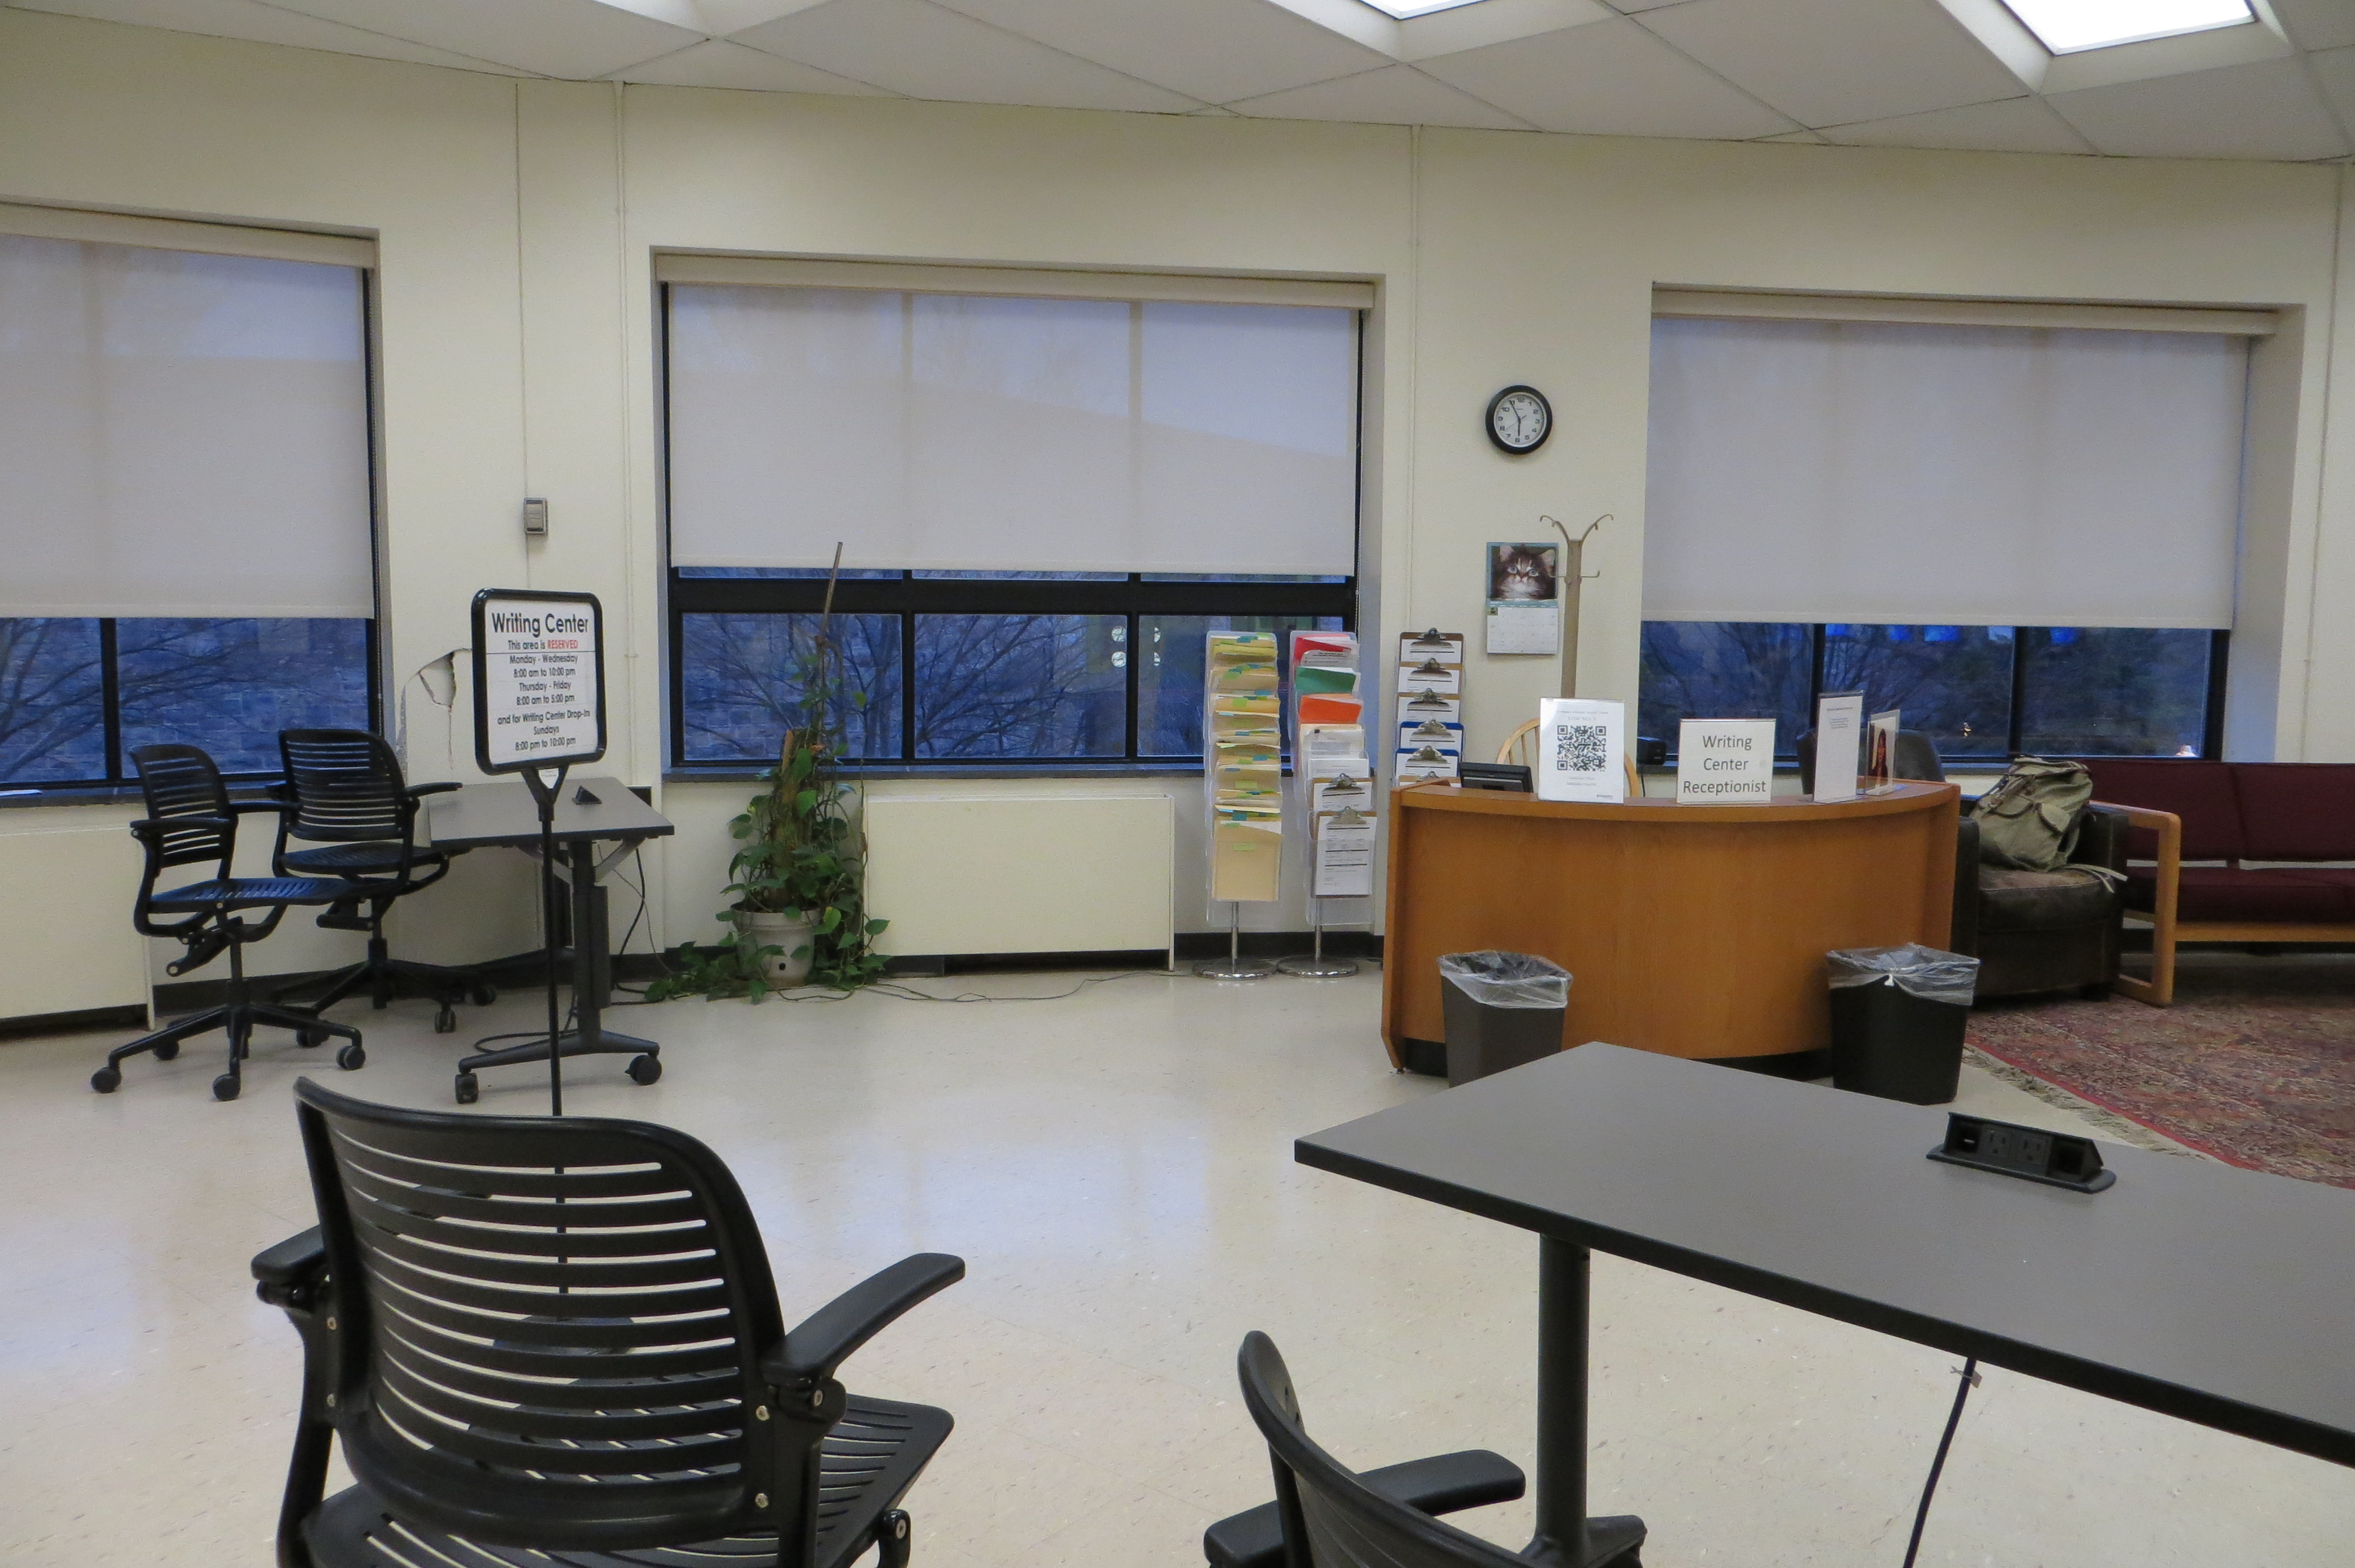
\includegraphics[width=0.75\linewidth]{WC4}
  \caption{}
  \label{fig:WC4}
  \end{subfigure}\\[1ex]
  \begin{subfigure}{.5\linewidth}
  \centering
  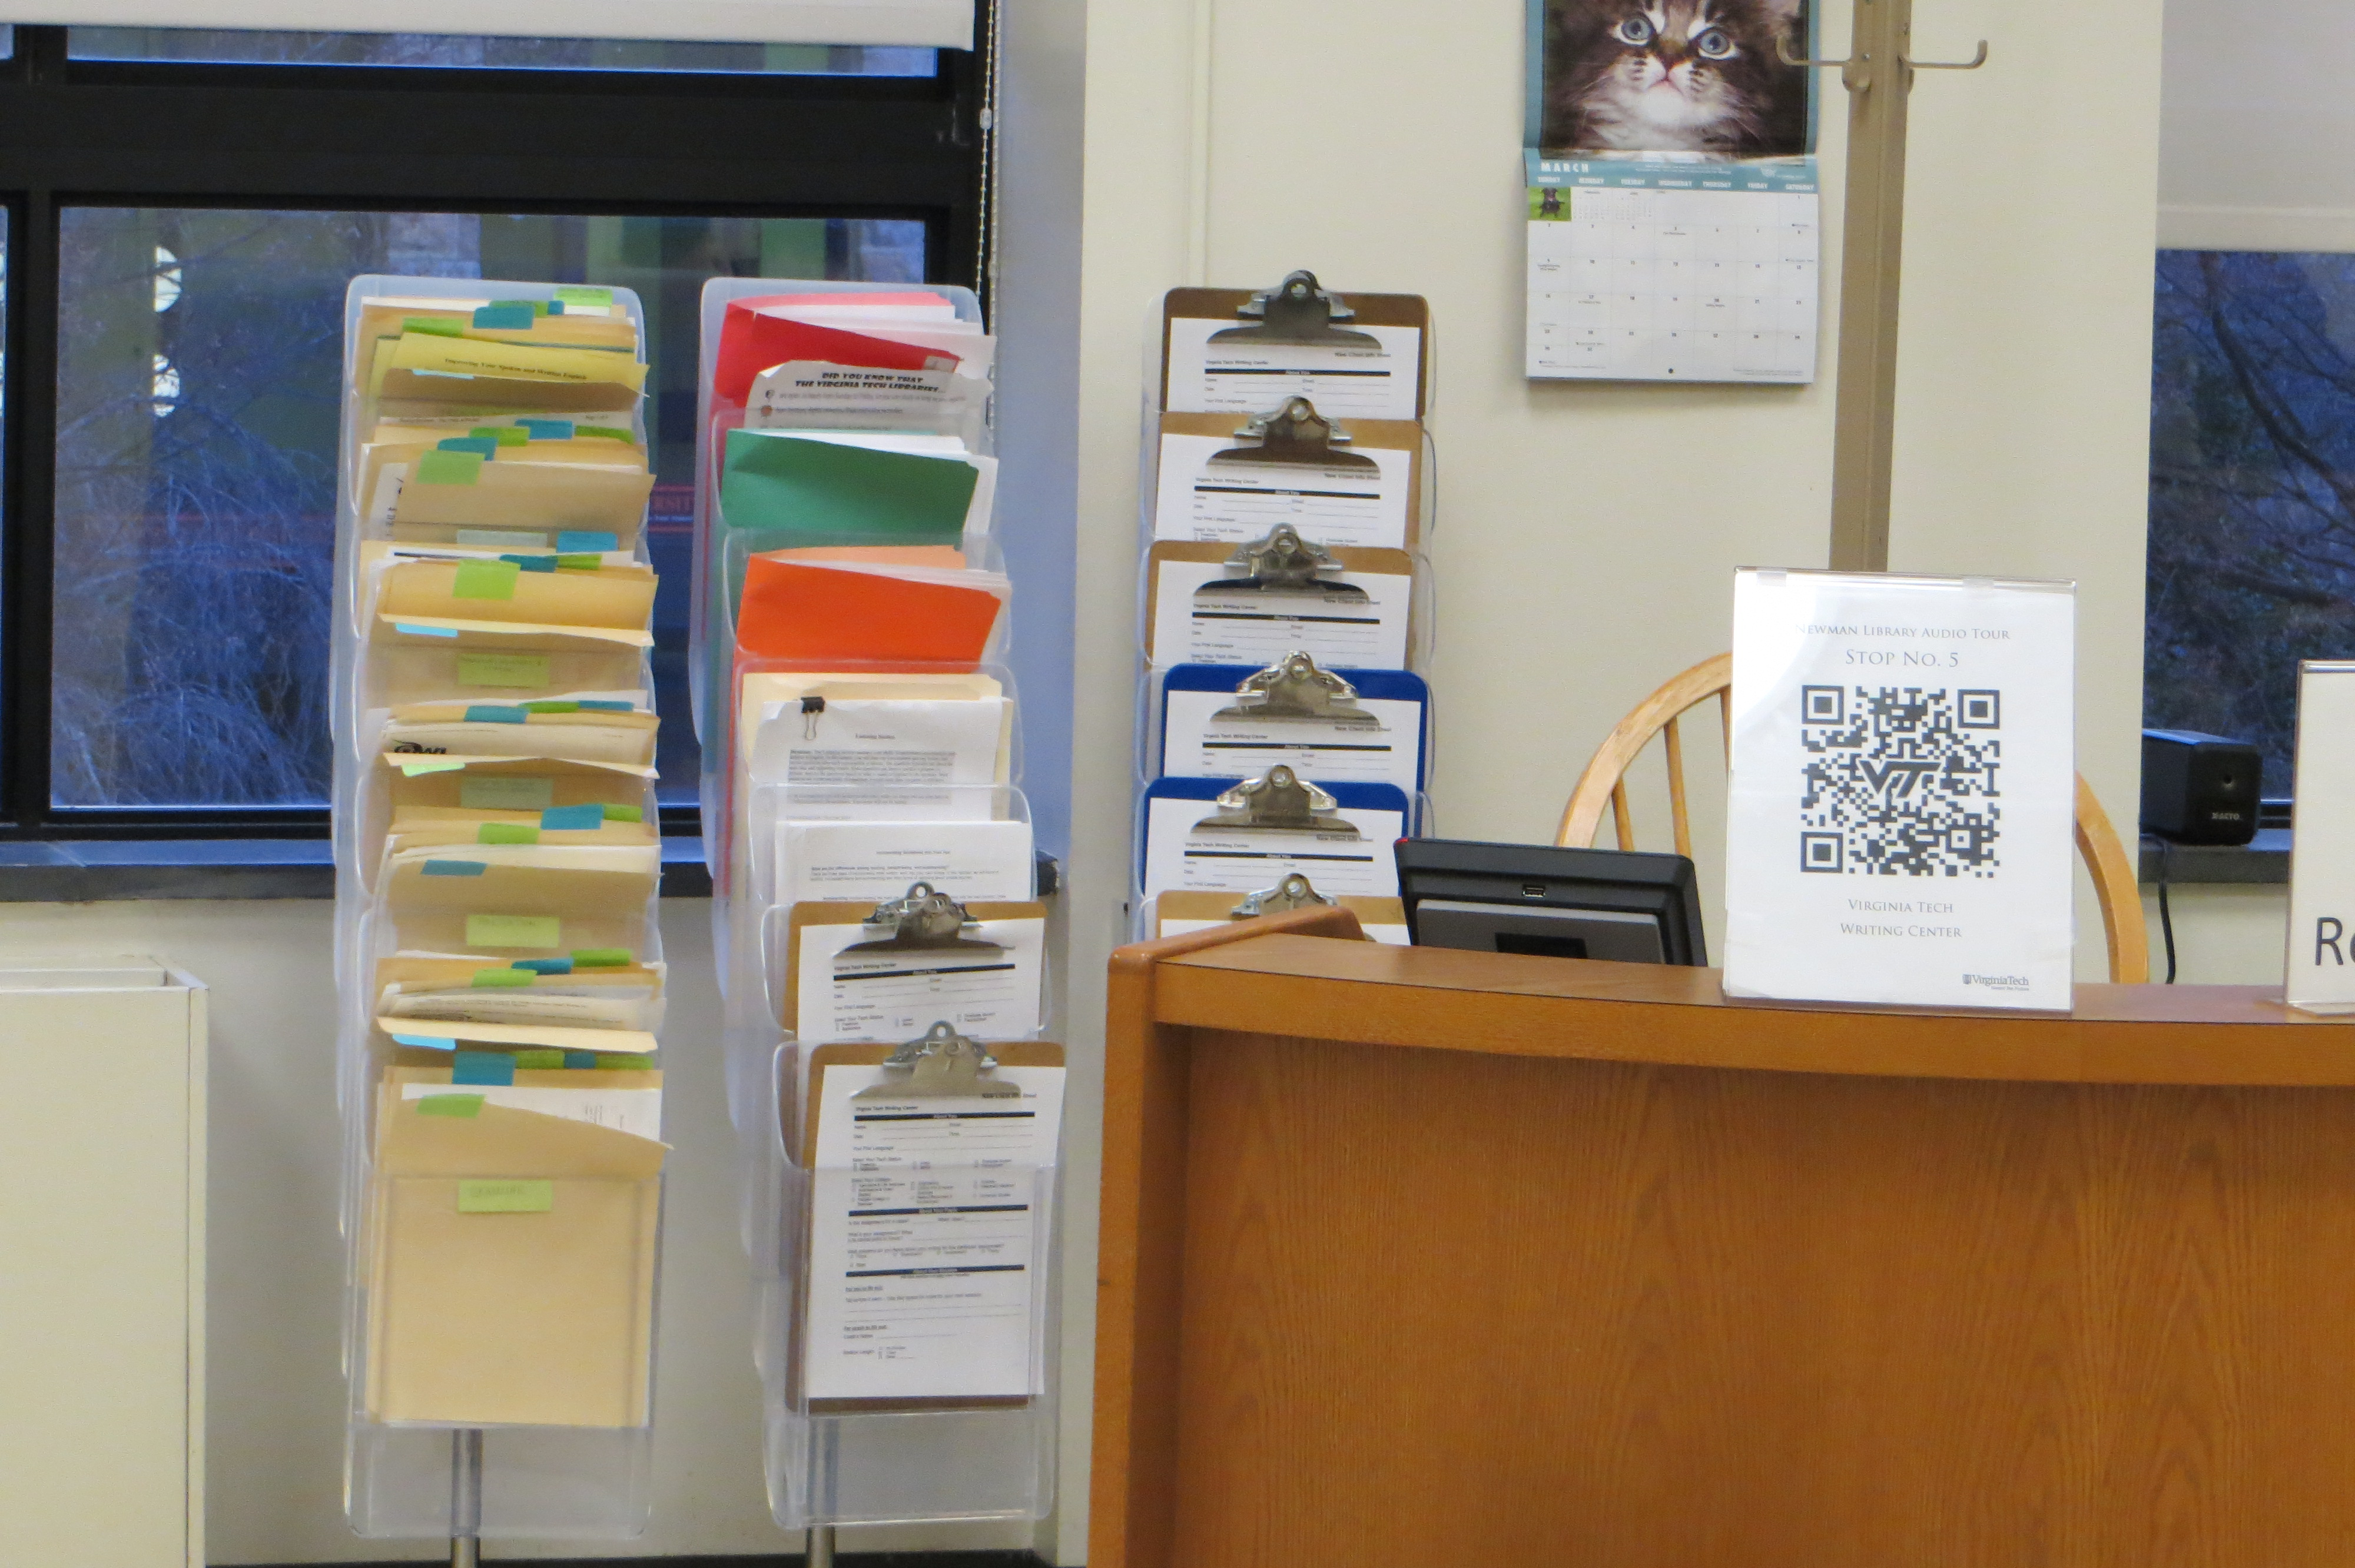
\includegraphics[width=0.75\linewidth]{WC5}
  \caption{}
  \label{fig:WC5}
  \end{subfigure}%
  \begin{subfigure}{.5\linewidth}
  \centering
  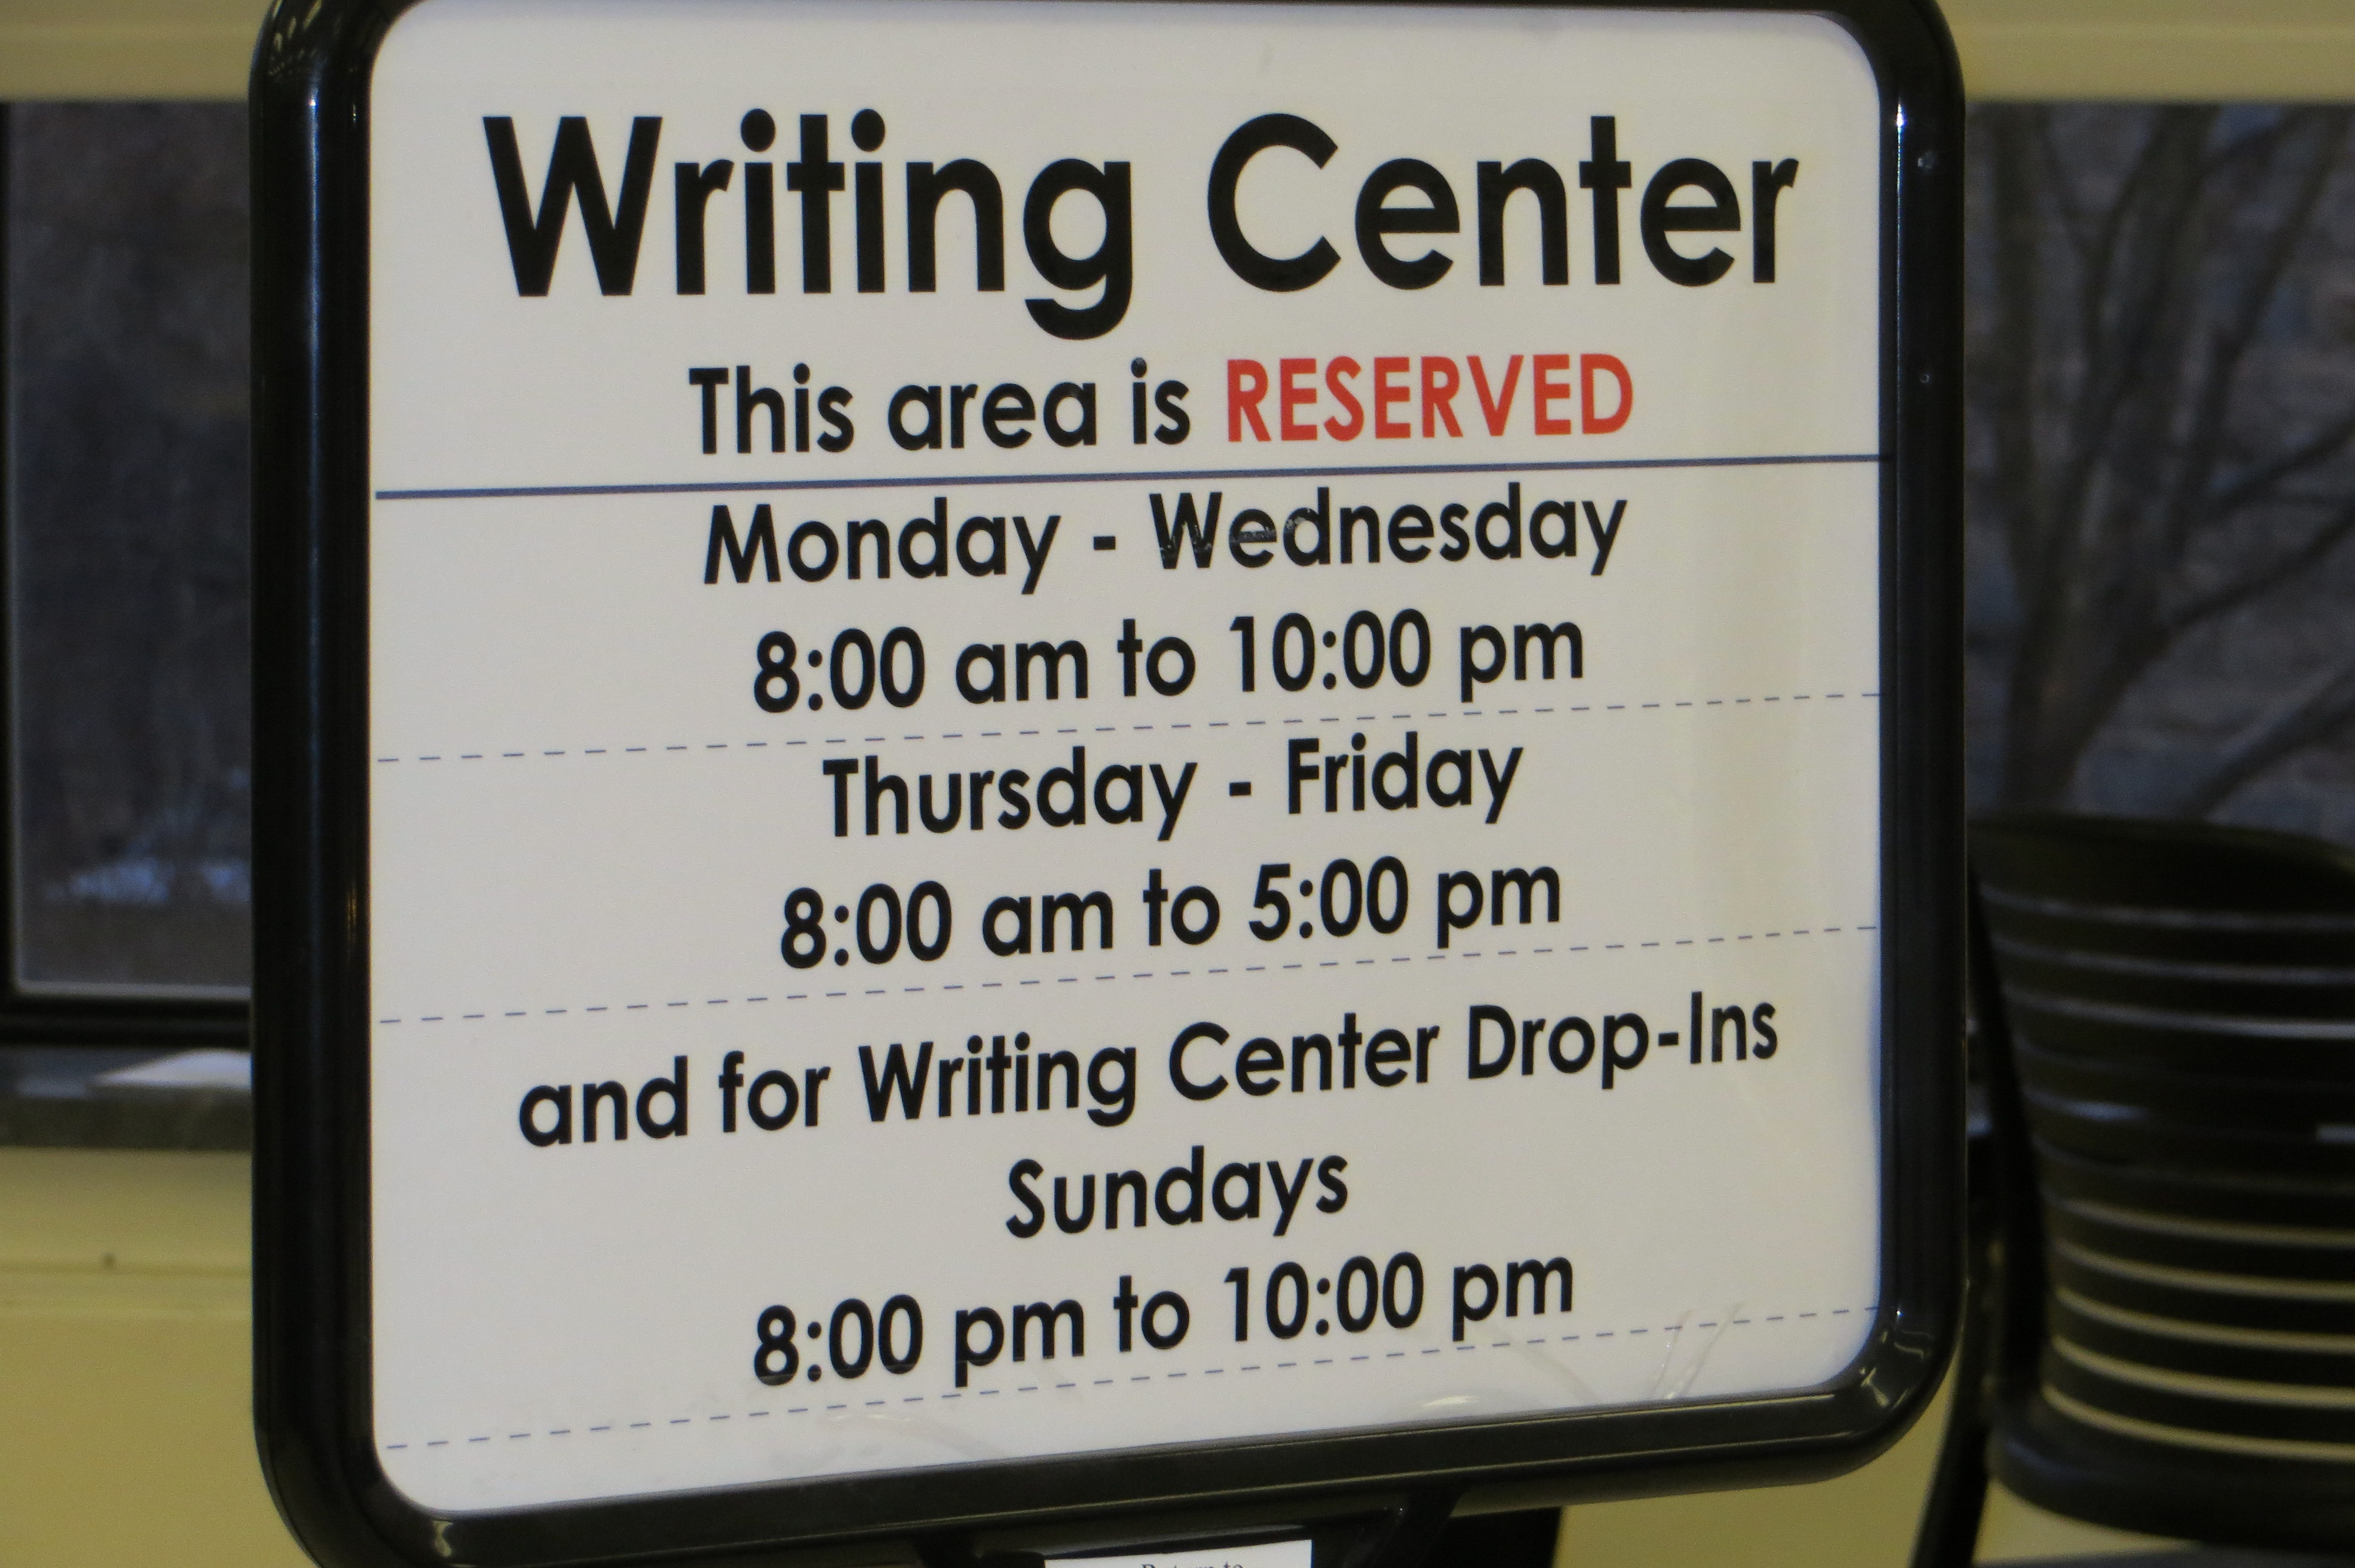
\includegraphics[width=0.75\linewidth]{WC6}
  \caption{}
  \label{fig:WC6}
  \end{subfigure}\\[1ex]
  \begin{subfigure}{.5\linewidth}
  \centering
  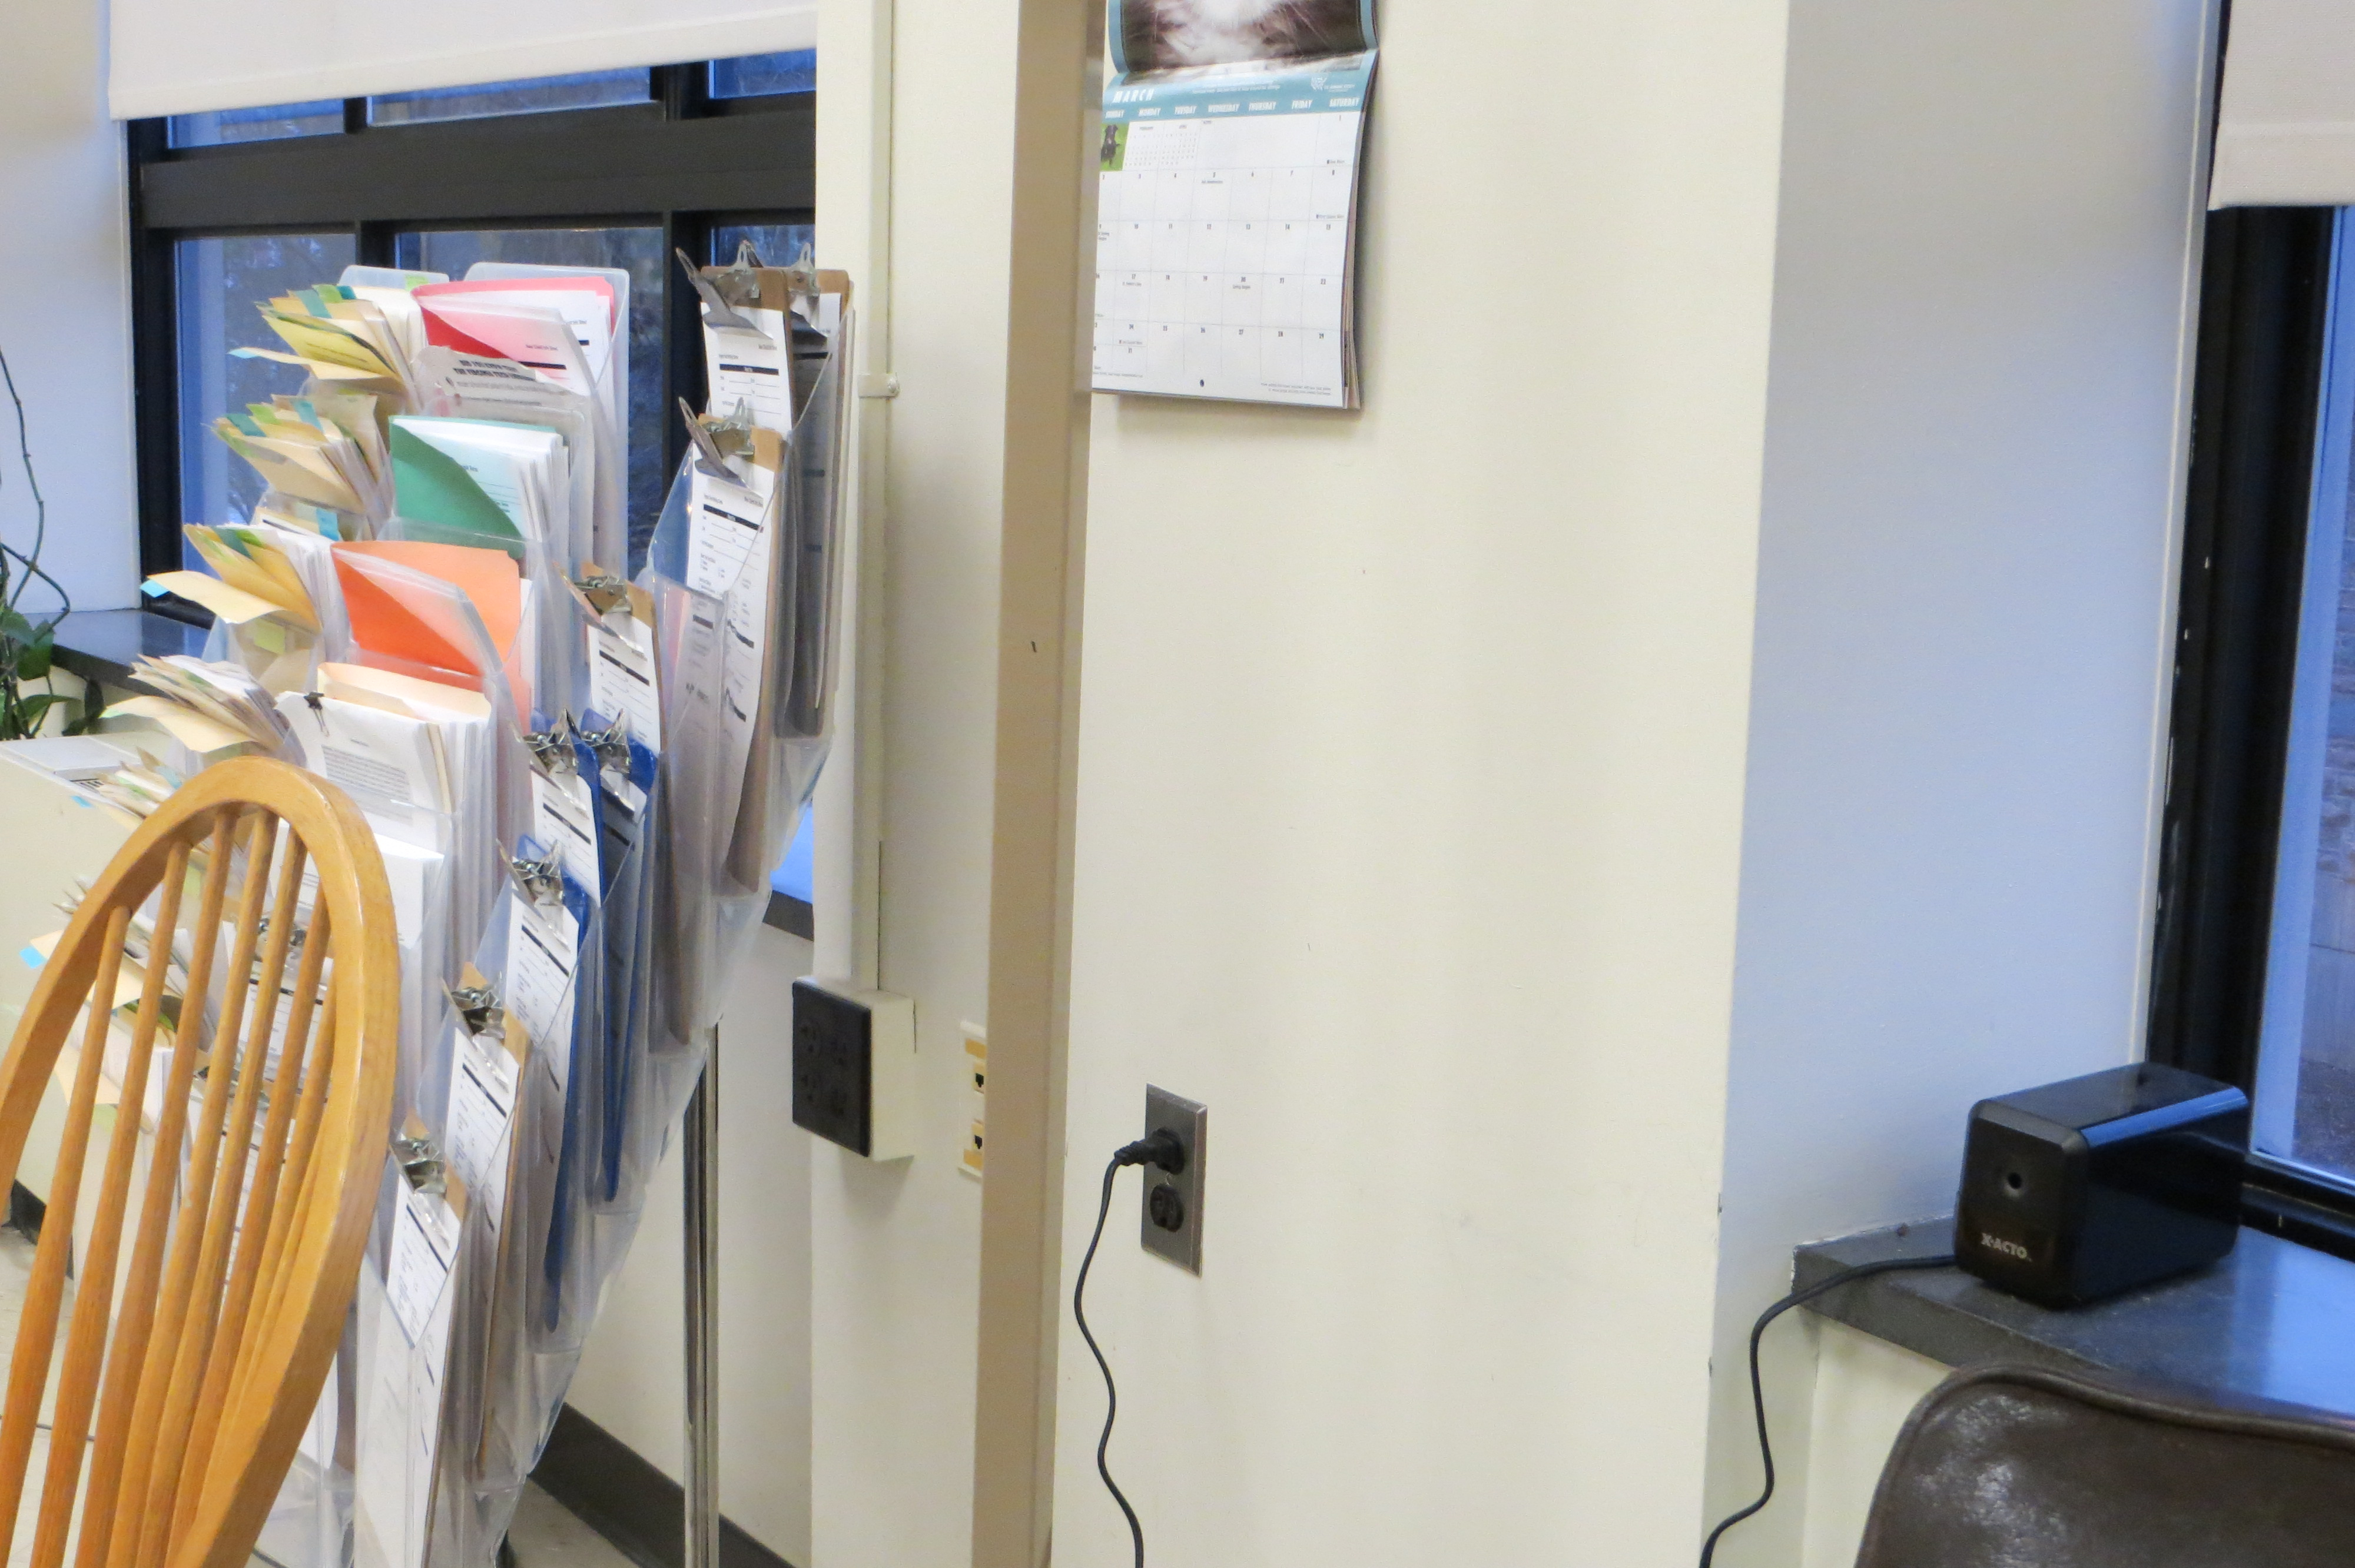
\includegraphics[width=0.75\linewidth]{WC7}
  \caption{}
  \label{fig:WC7}
  \end{subfigure}%
  \begin{subfigure}{.5\linewidth}
  \centering
  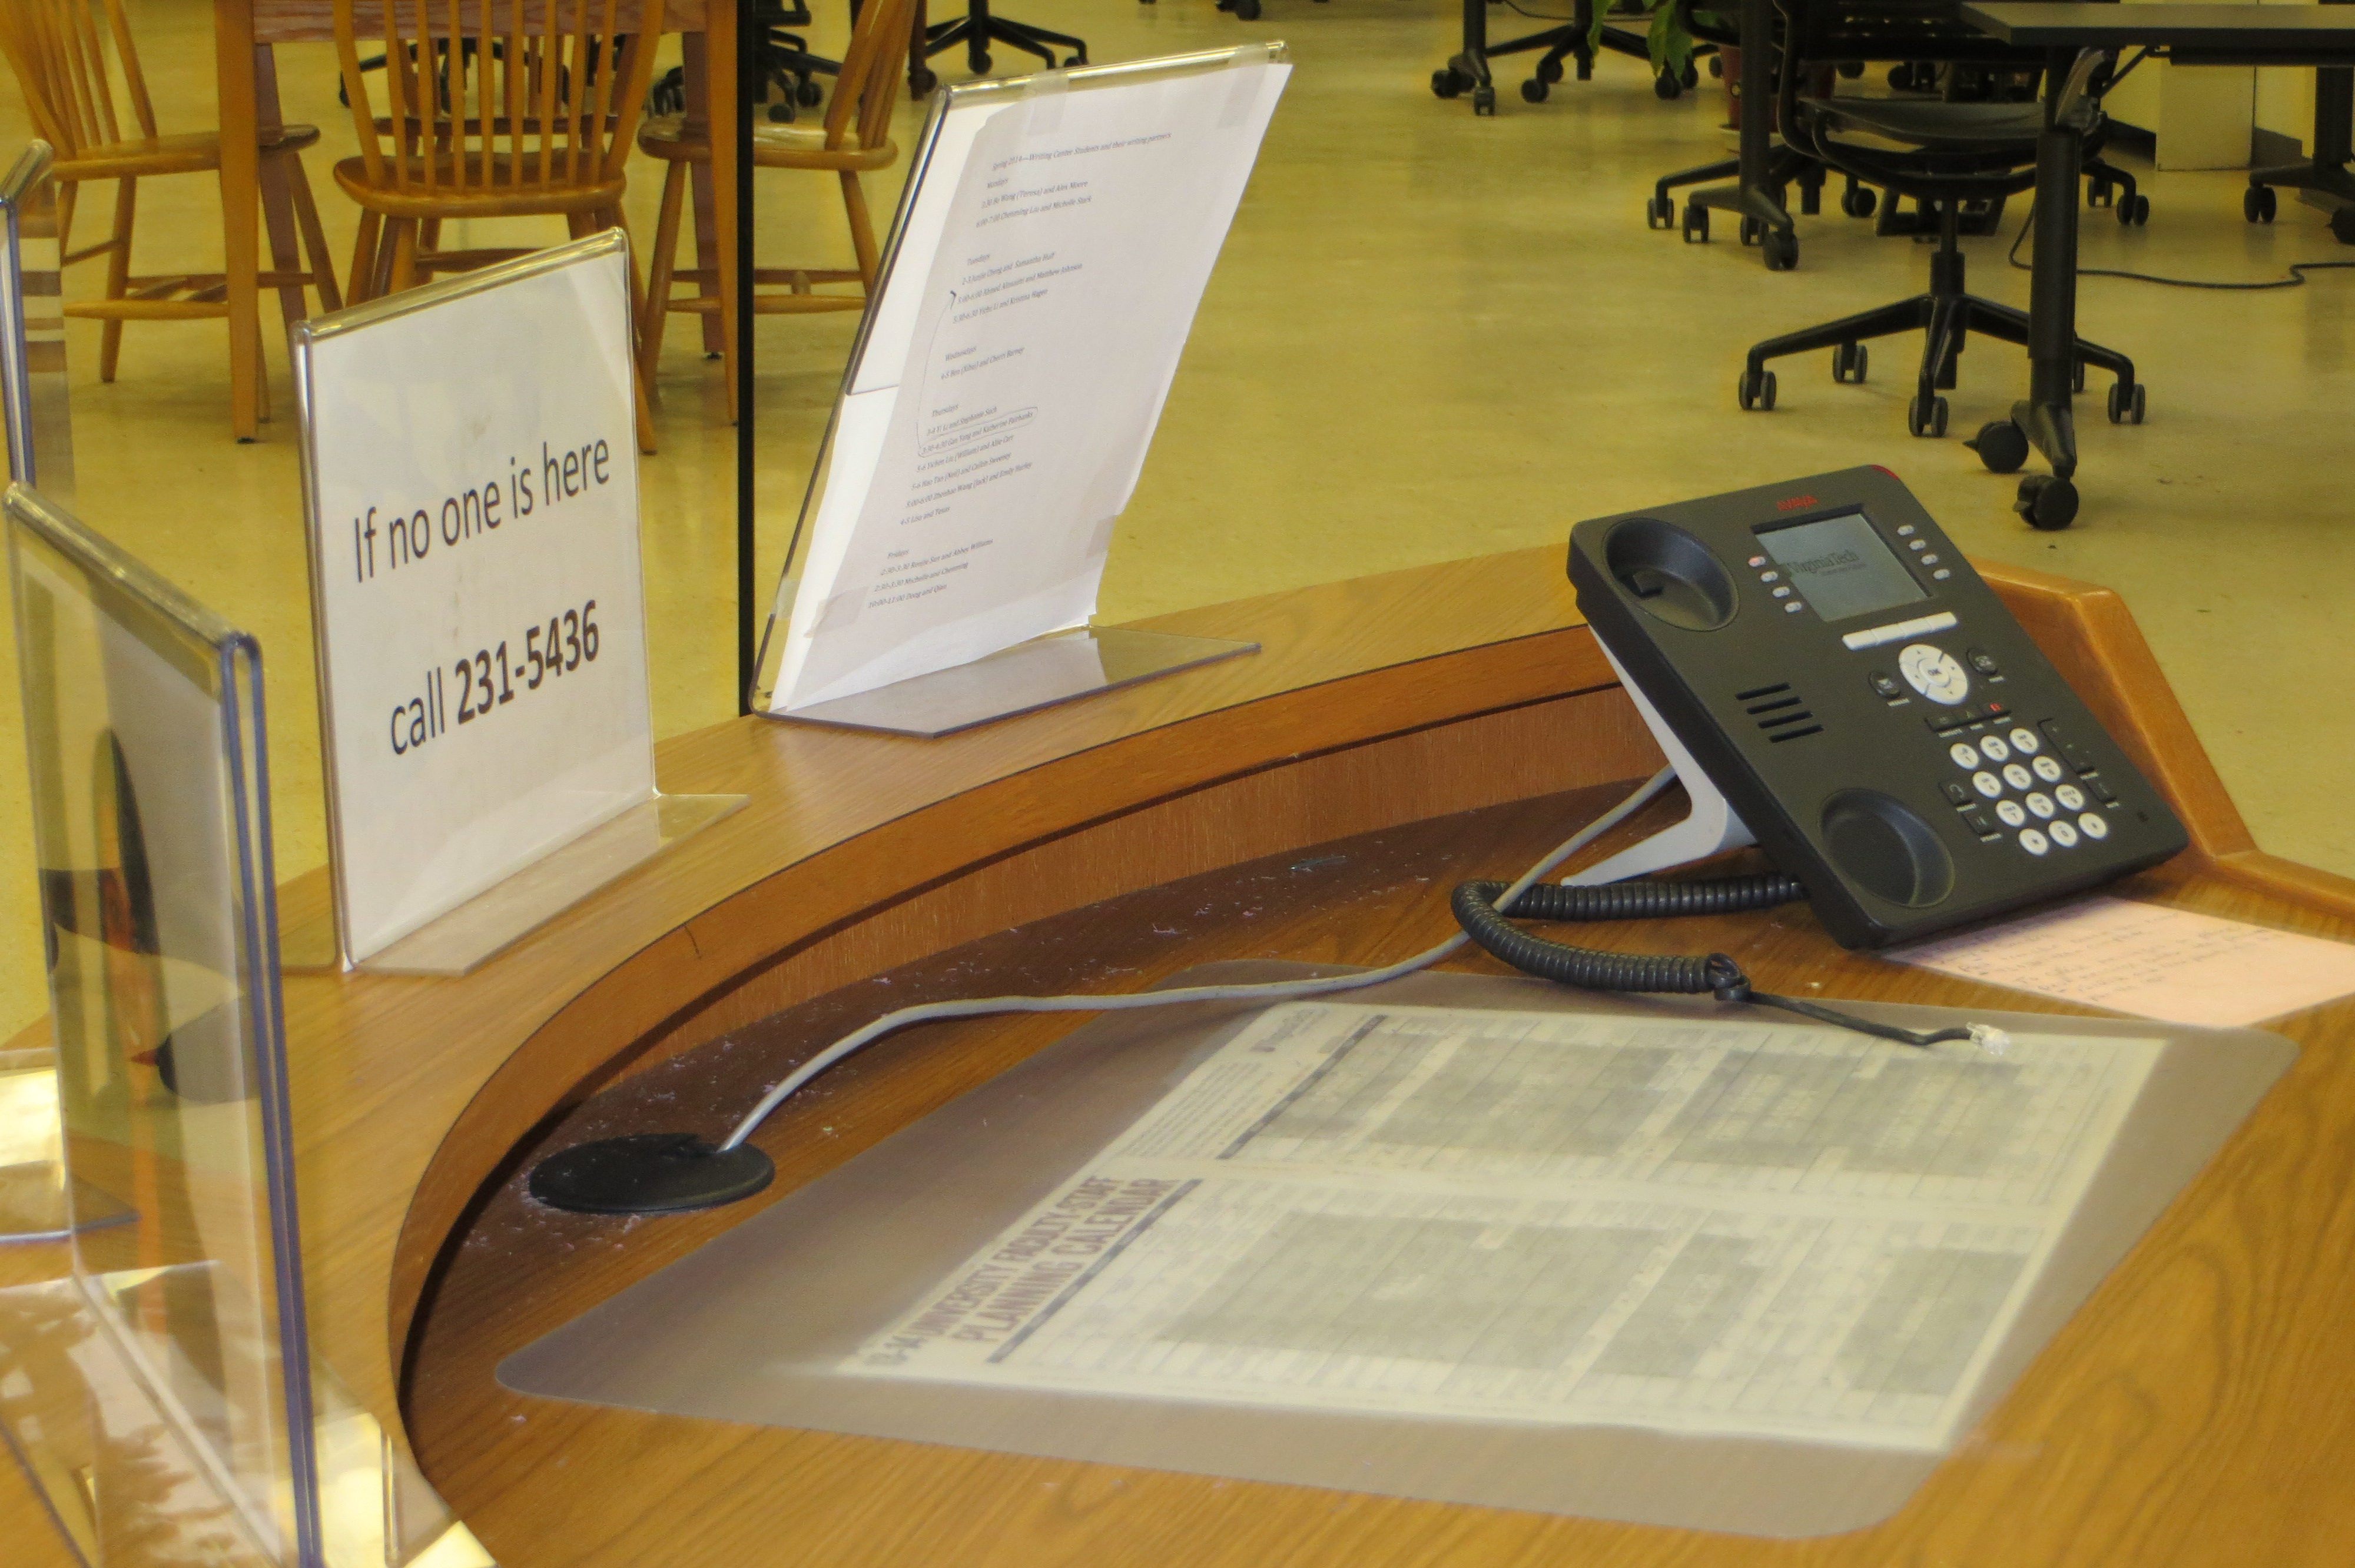
\includegraphics[width=0.75\linewidth]{WC8}
  \caption{}
  \label{fig:WC8}
  \end{subfigure}
  \caption{The Writing Center.}
  \label{fig:TheWritingCenter}
  \end{figure}
\end{samepage}

\section{Sketches} %10
% Show scans of any sketches you made in the field
  We did not make any field sketches.

\section{Task Data} %11
% Give samples of task data and other data you collected.
  Documents handled by people in the WC are noted as \textcolor{pink}{pink} squares in the work flow figure of \ref{fig:Workflow_final}.

\section{Raw Data and Work Activity Notes} %12
% Show samples ( a dozen or so) of your raw data notes and the corresponding work activity notes you extracted.
  \subsection*{Audio Interview Notes} % Sub-sub-section
  \href{http://www.dropbox.specialorange.com/vt/5714%20UX/}{Audio Folder}\\
    \href{http://www.dropbox.specialorange.com/vt/5714%20UX/ADir1.aac}{Assistant Director 1}\\
    \href{http://www.dropbox.specialorange.com/vt/5714%20UX/C1.aac}{Coach 1}\\

  \subsection*{Raw Data Notes}
  
  \begin{figure}[H]
  \centering
  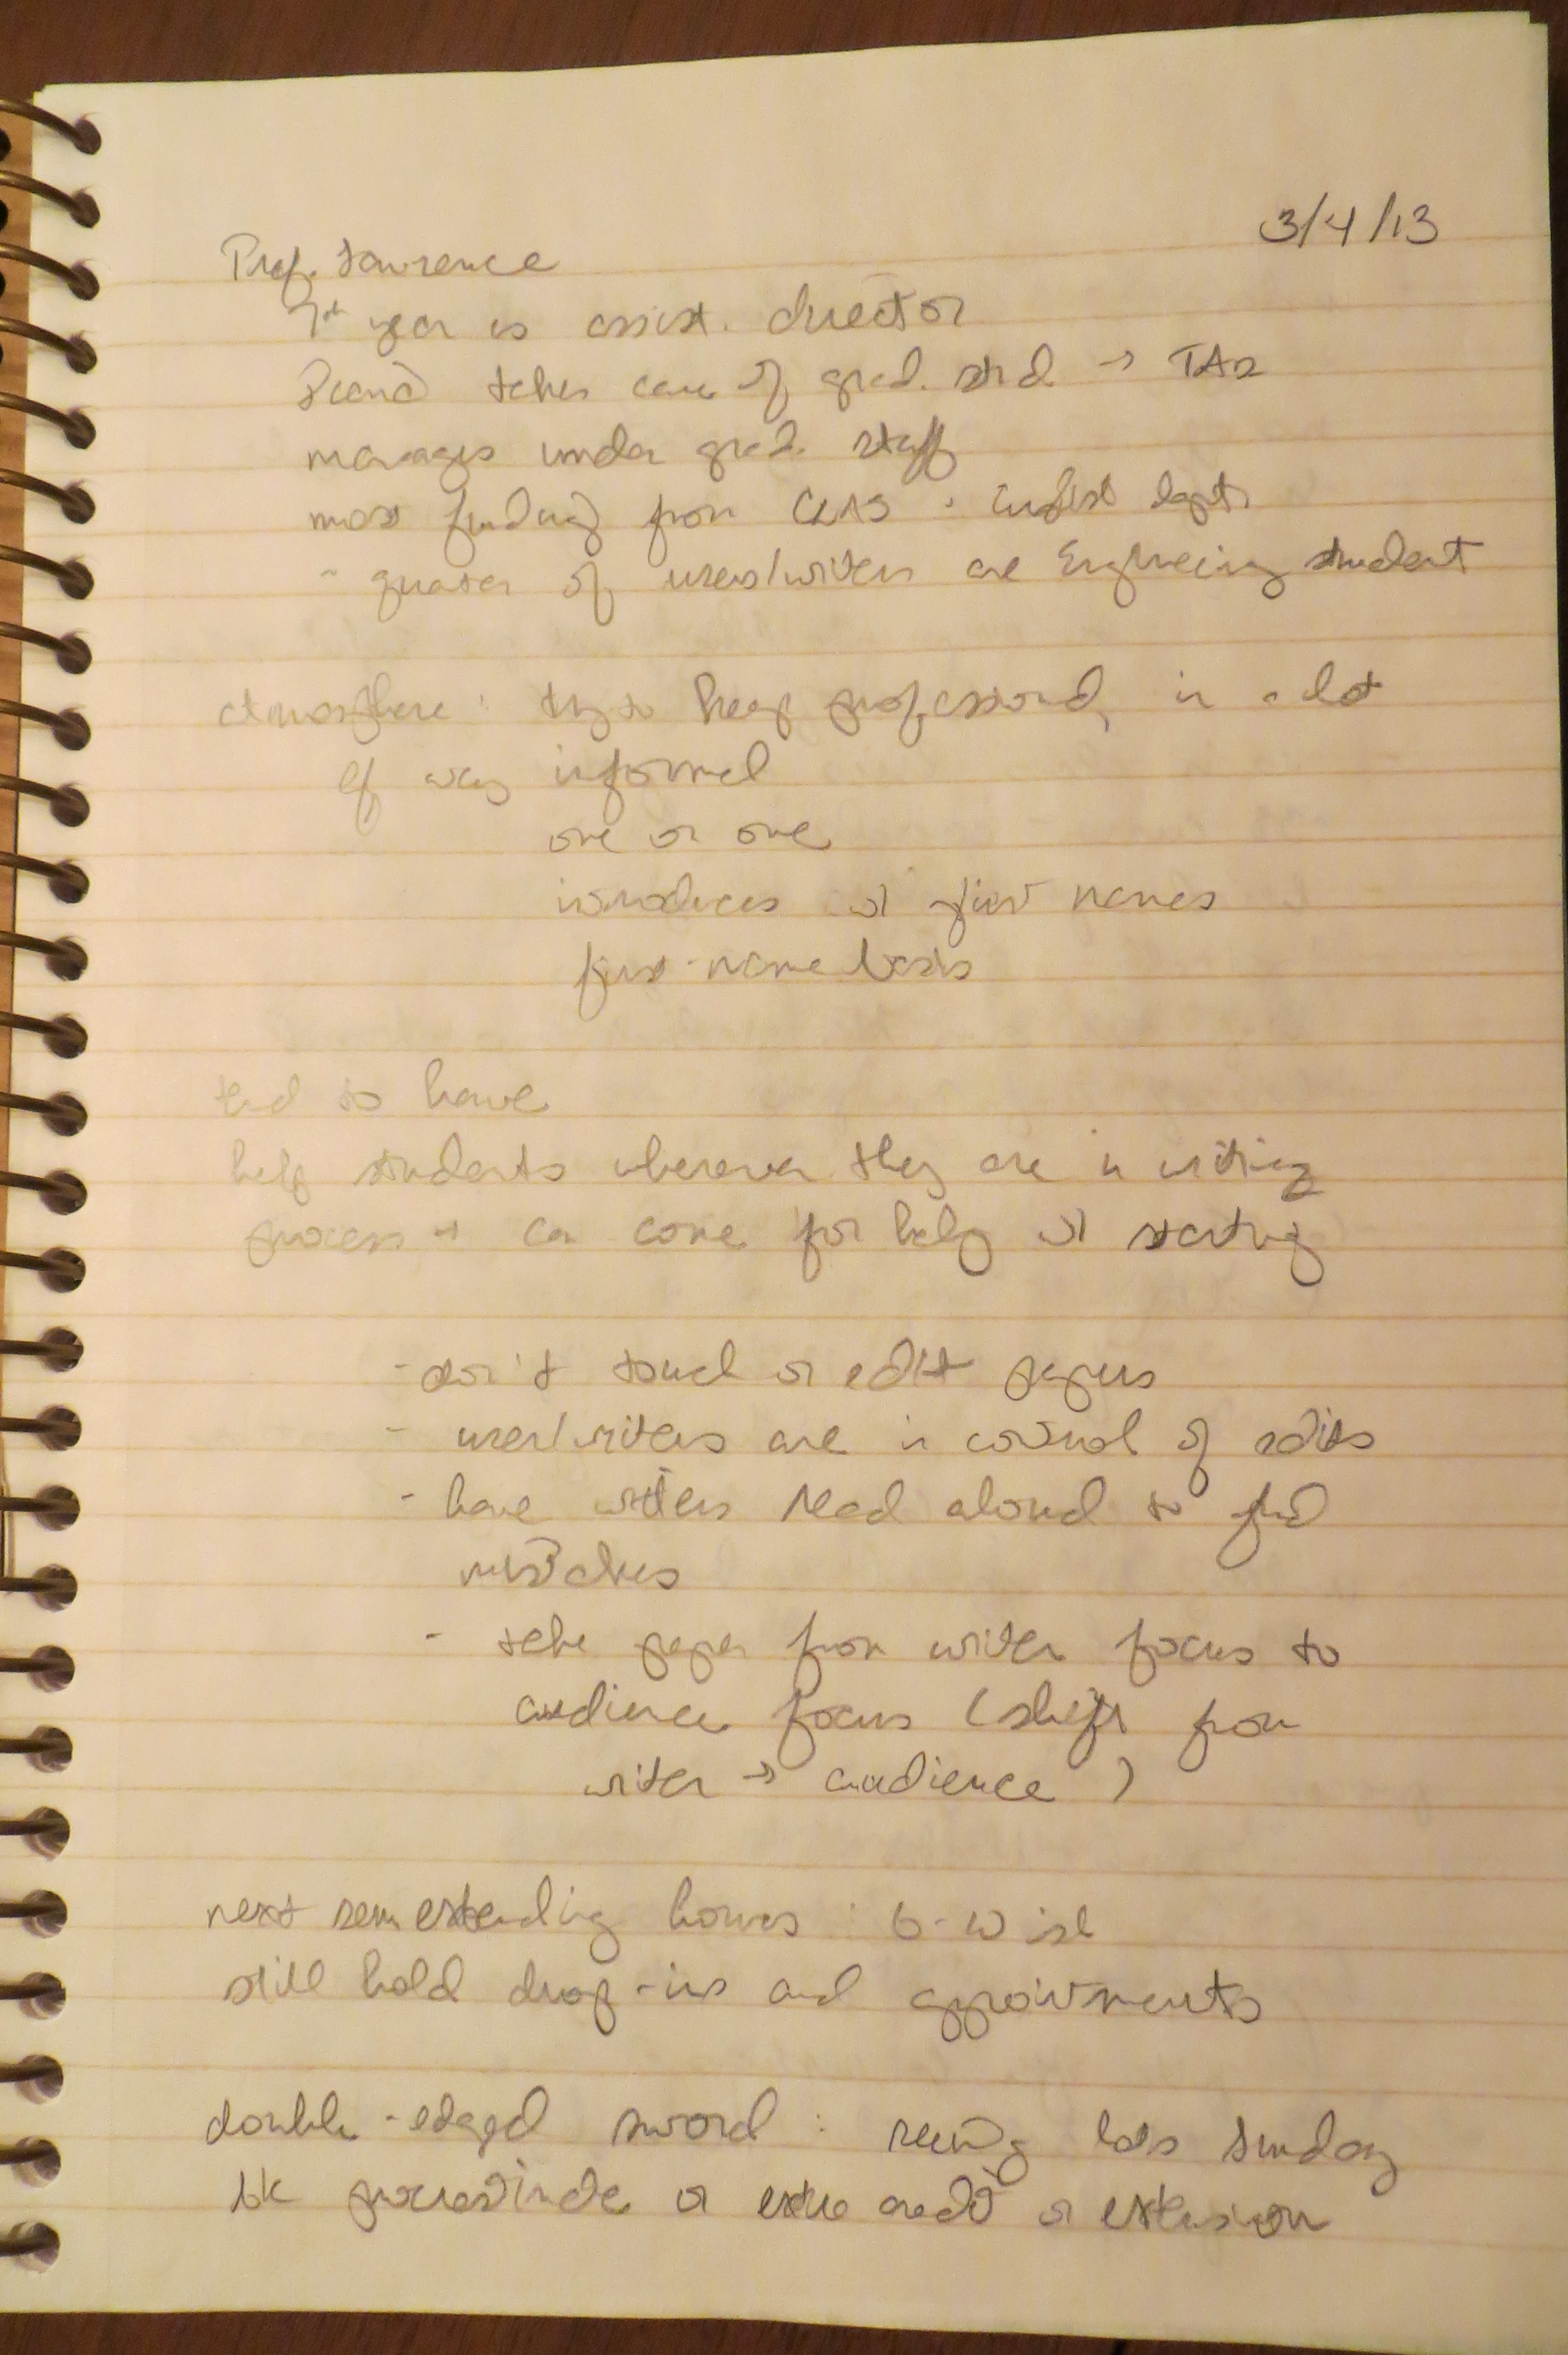
\includegraphics[width=0.75\linewidth]{RAZ_raw_notes1}
  \caption{}
  \label{fig:rn1}
  \end{figure}
  \begin{figure}[H]
  \centering
  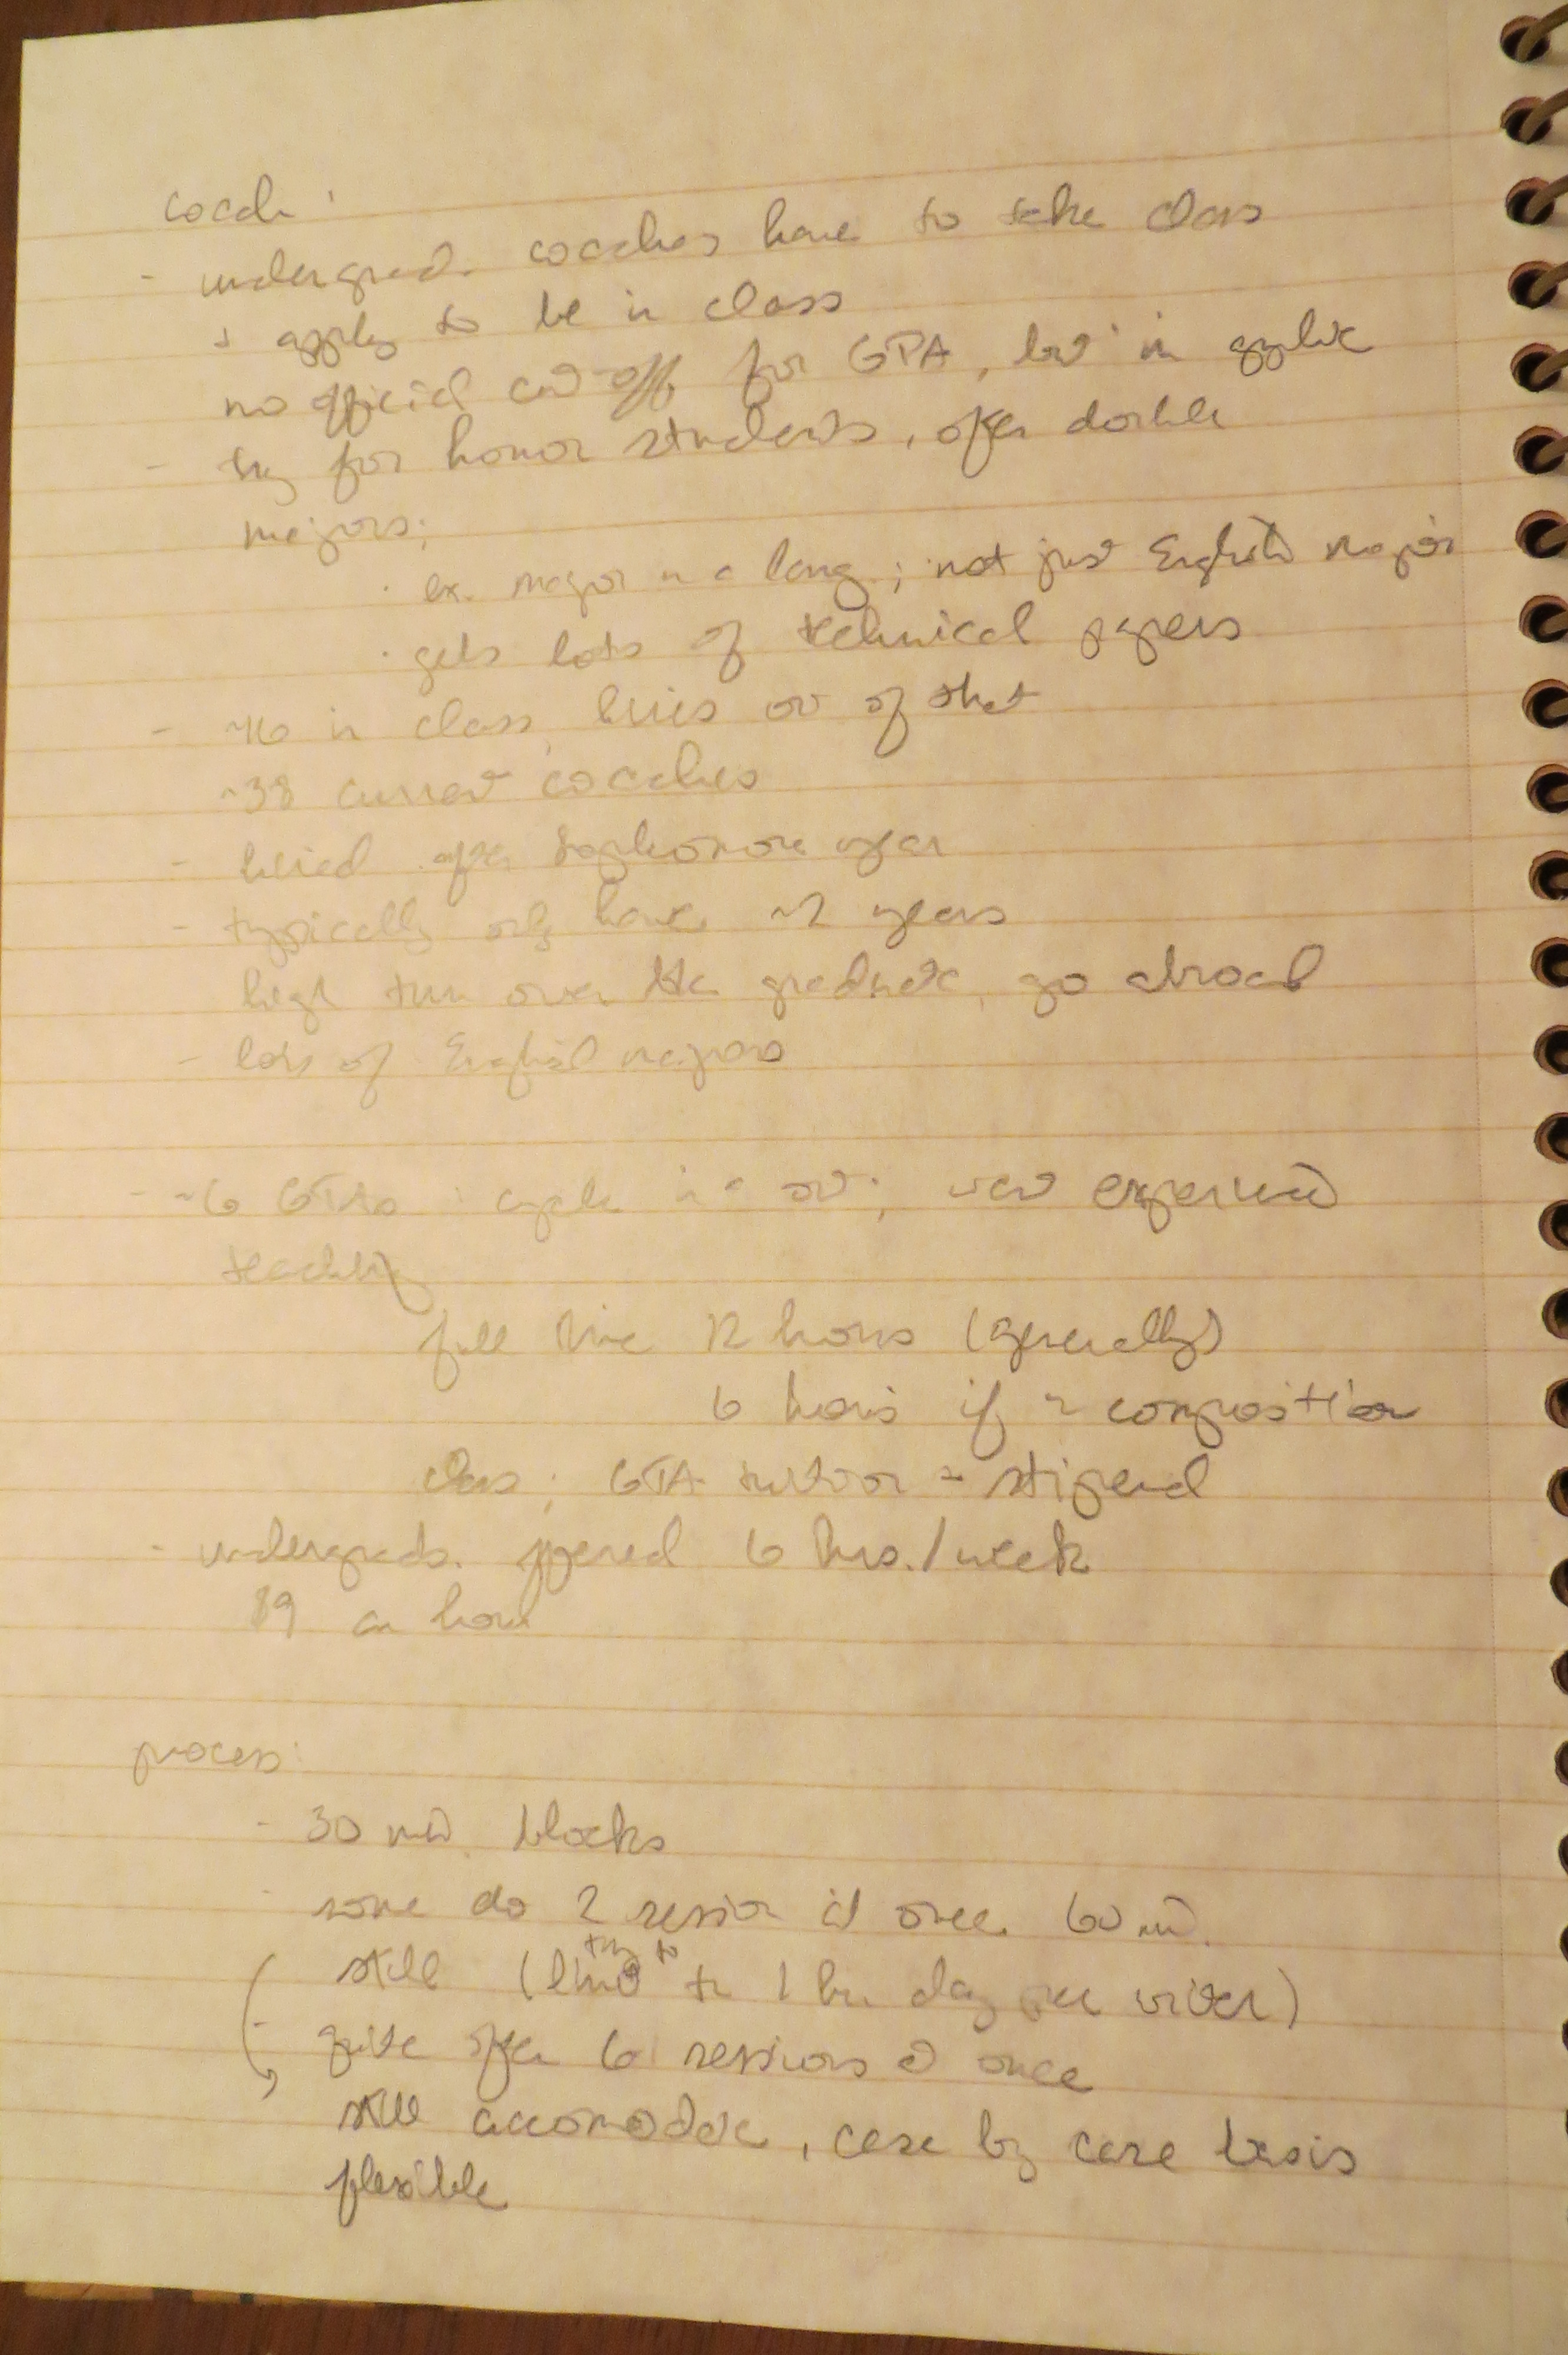
\includegraphics[width=0.75\linewidth]{RAZ_raw_notes2}
  \caption{}
  \label{fig:rn2}
  \end{figure}
  \begin{figure}[H]
  \centering
  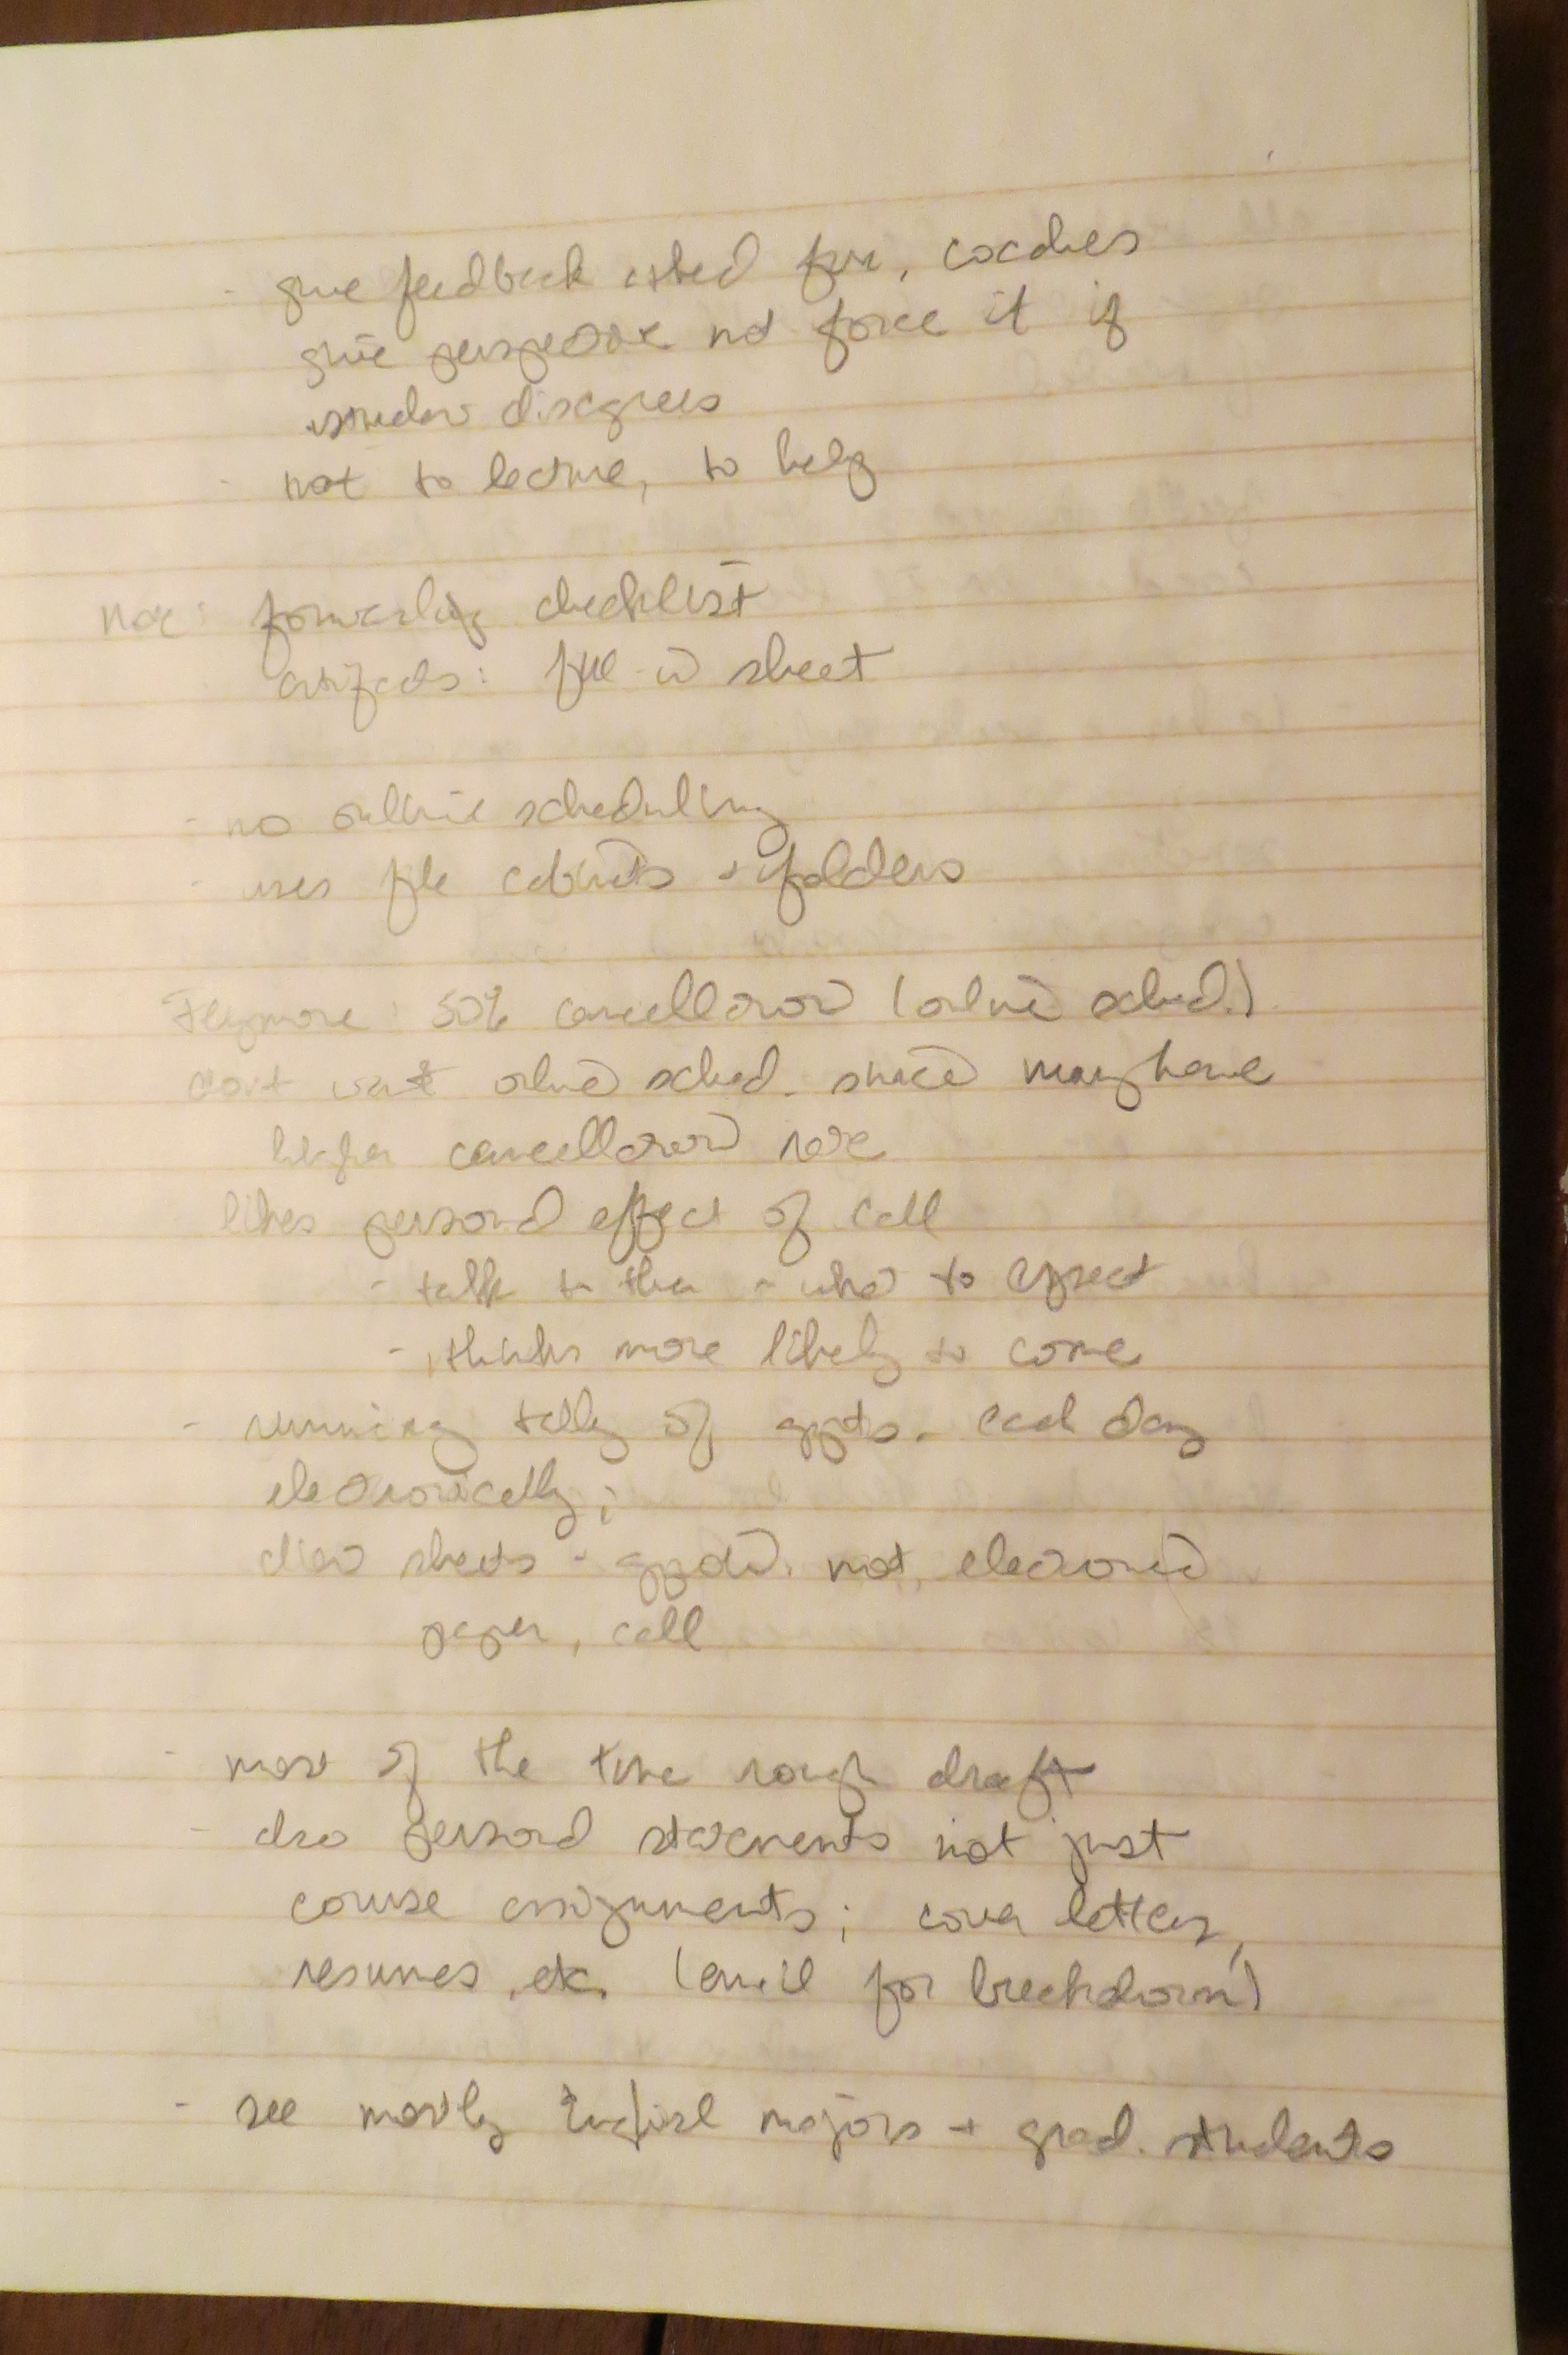
\includegraphics[width=0.75\linewidth]{RAZ_raw_notes3}
  \caption{}
  \label{fig:rn3}
  \end{figure}
  \begin{figure}[H]
  \centering
  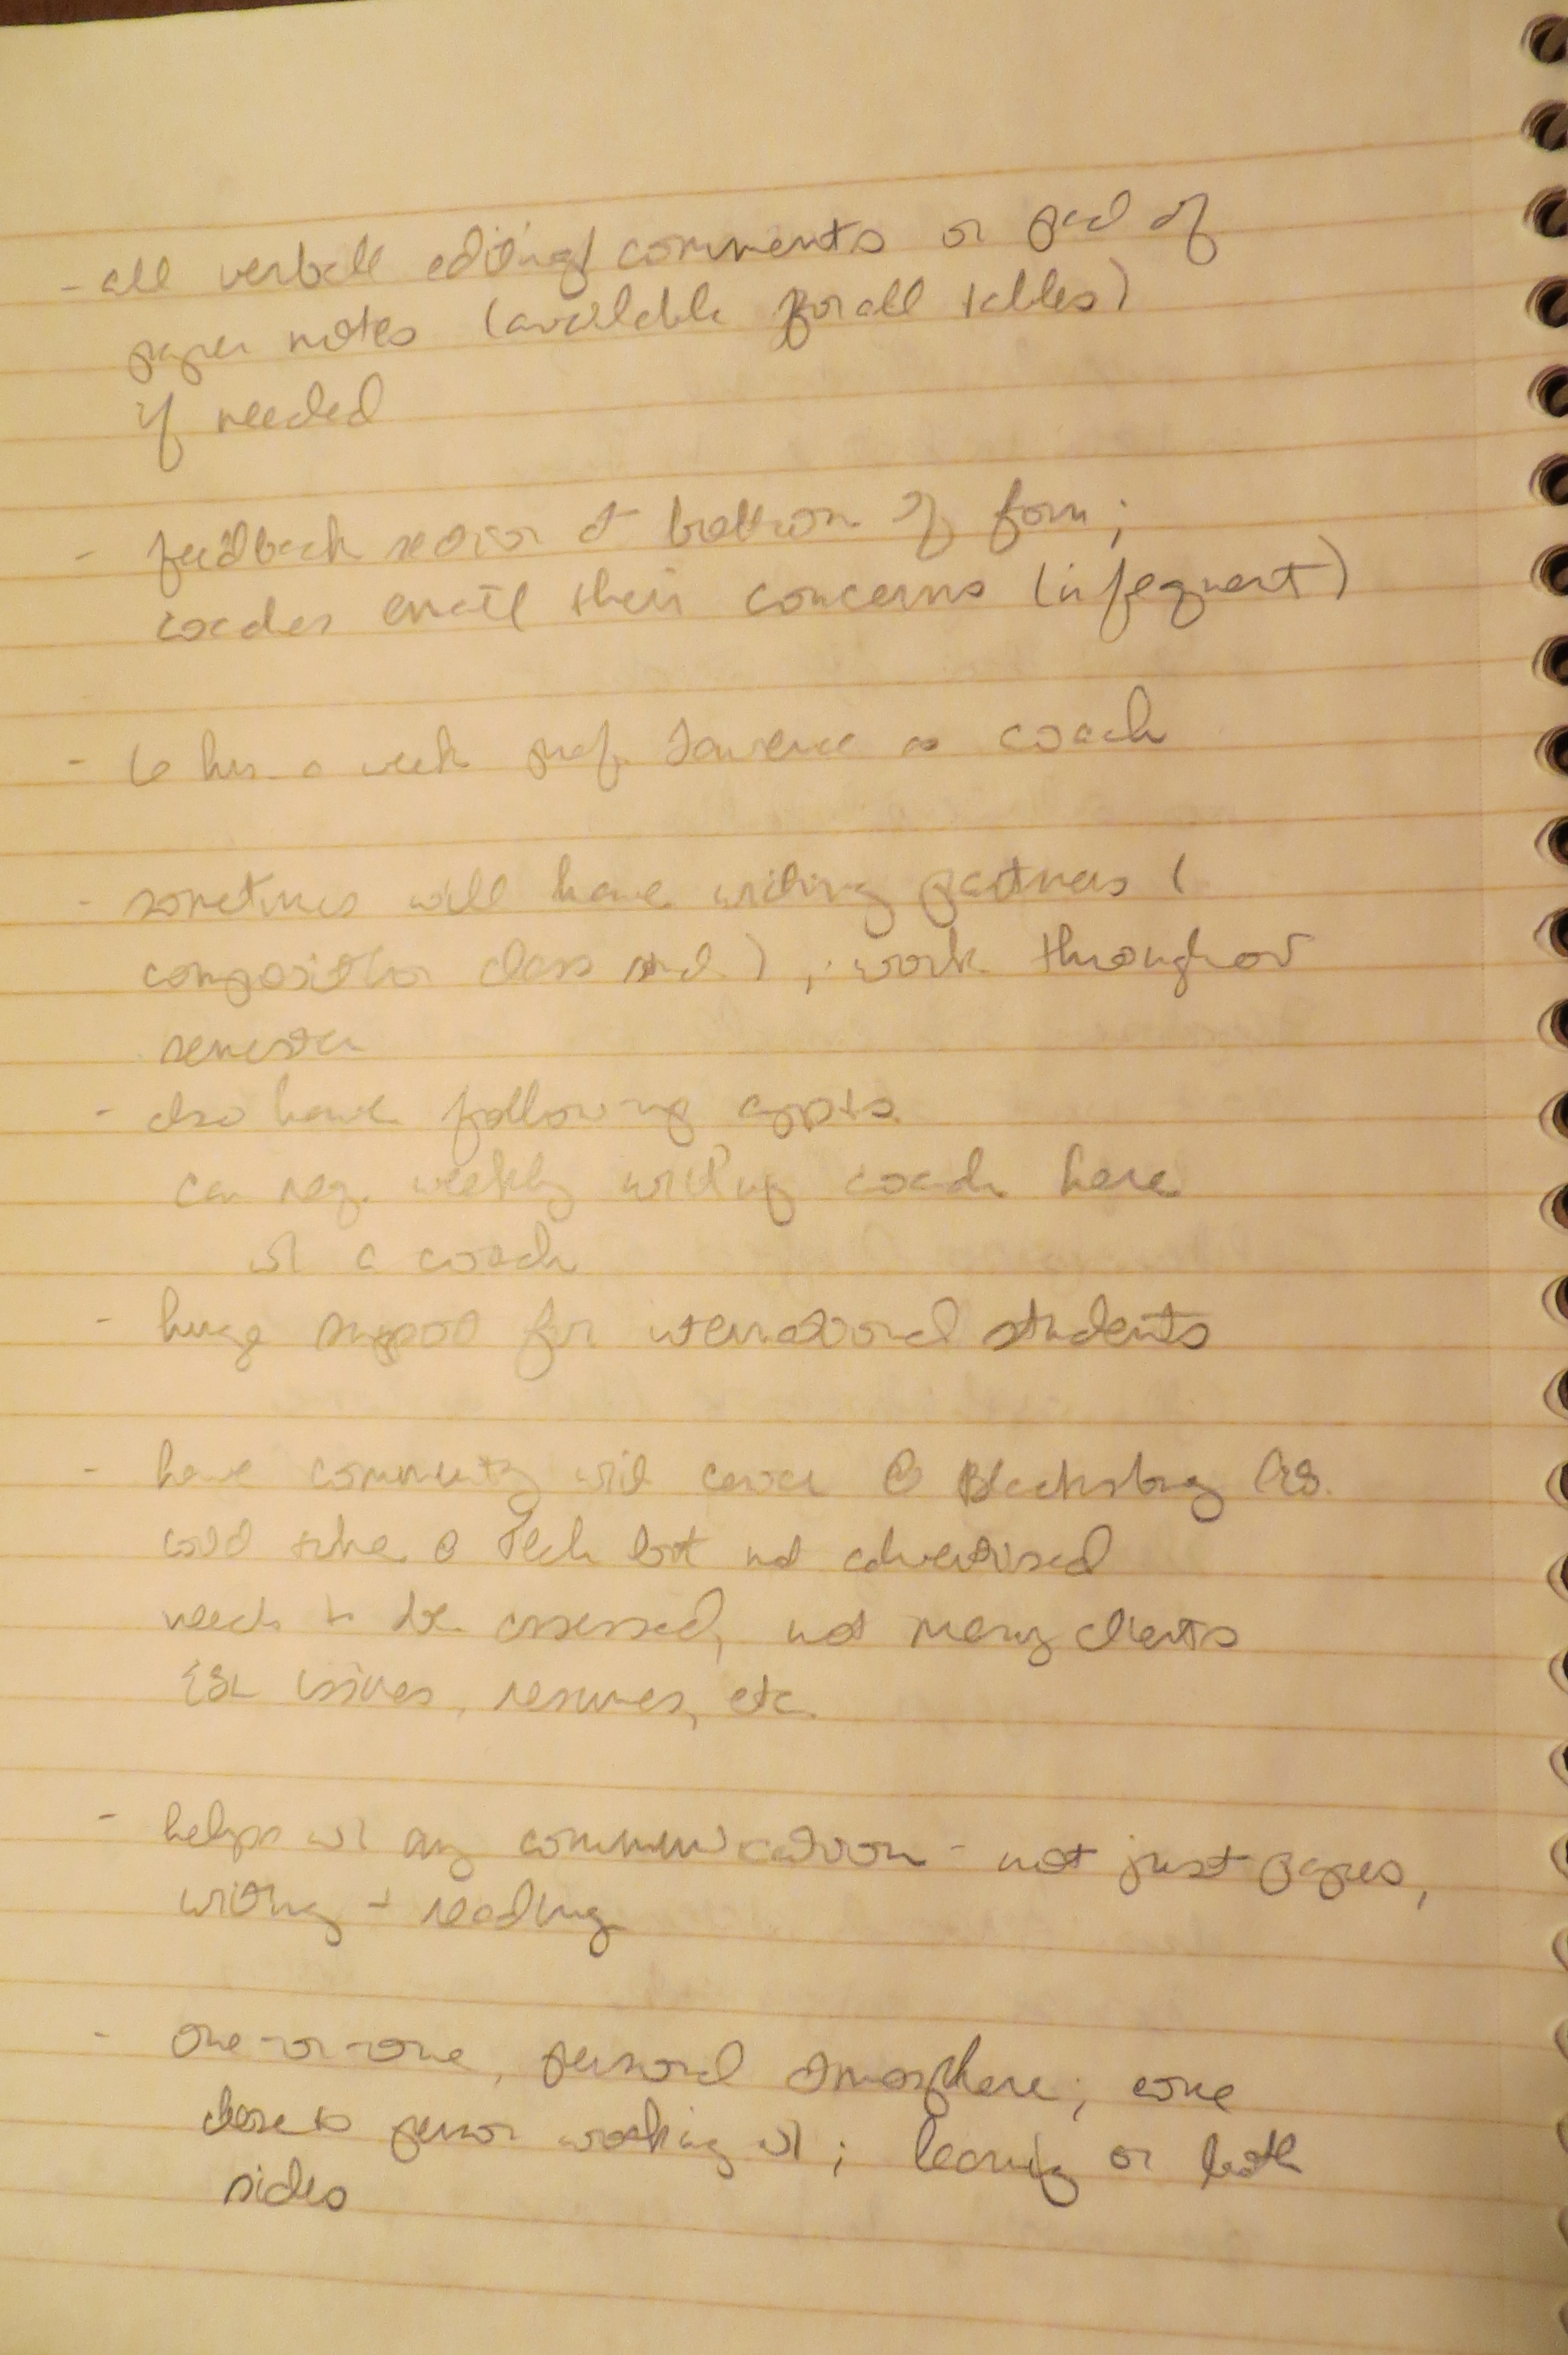
\includegraphics[width=0.75\linewidth]{RAZ_raw_notes4}
  \caption{}
  \label{fig:rn4}
  \end{figure}
  \begin{figure}[H]
  \centering
  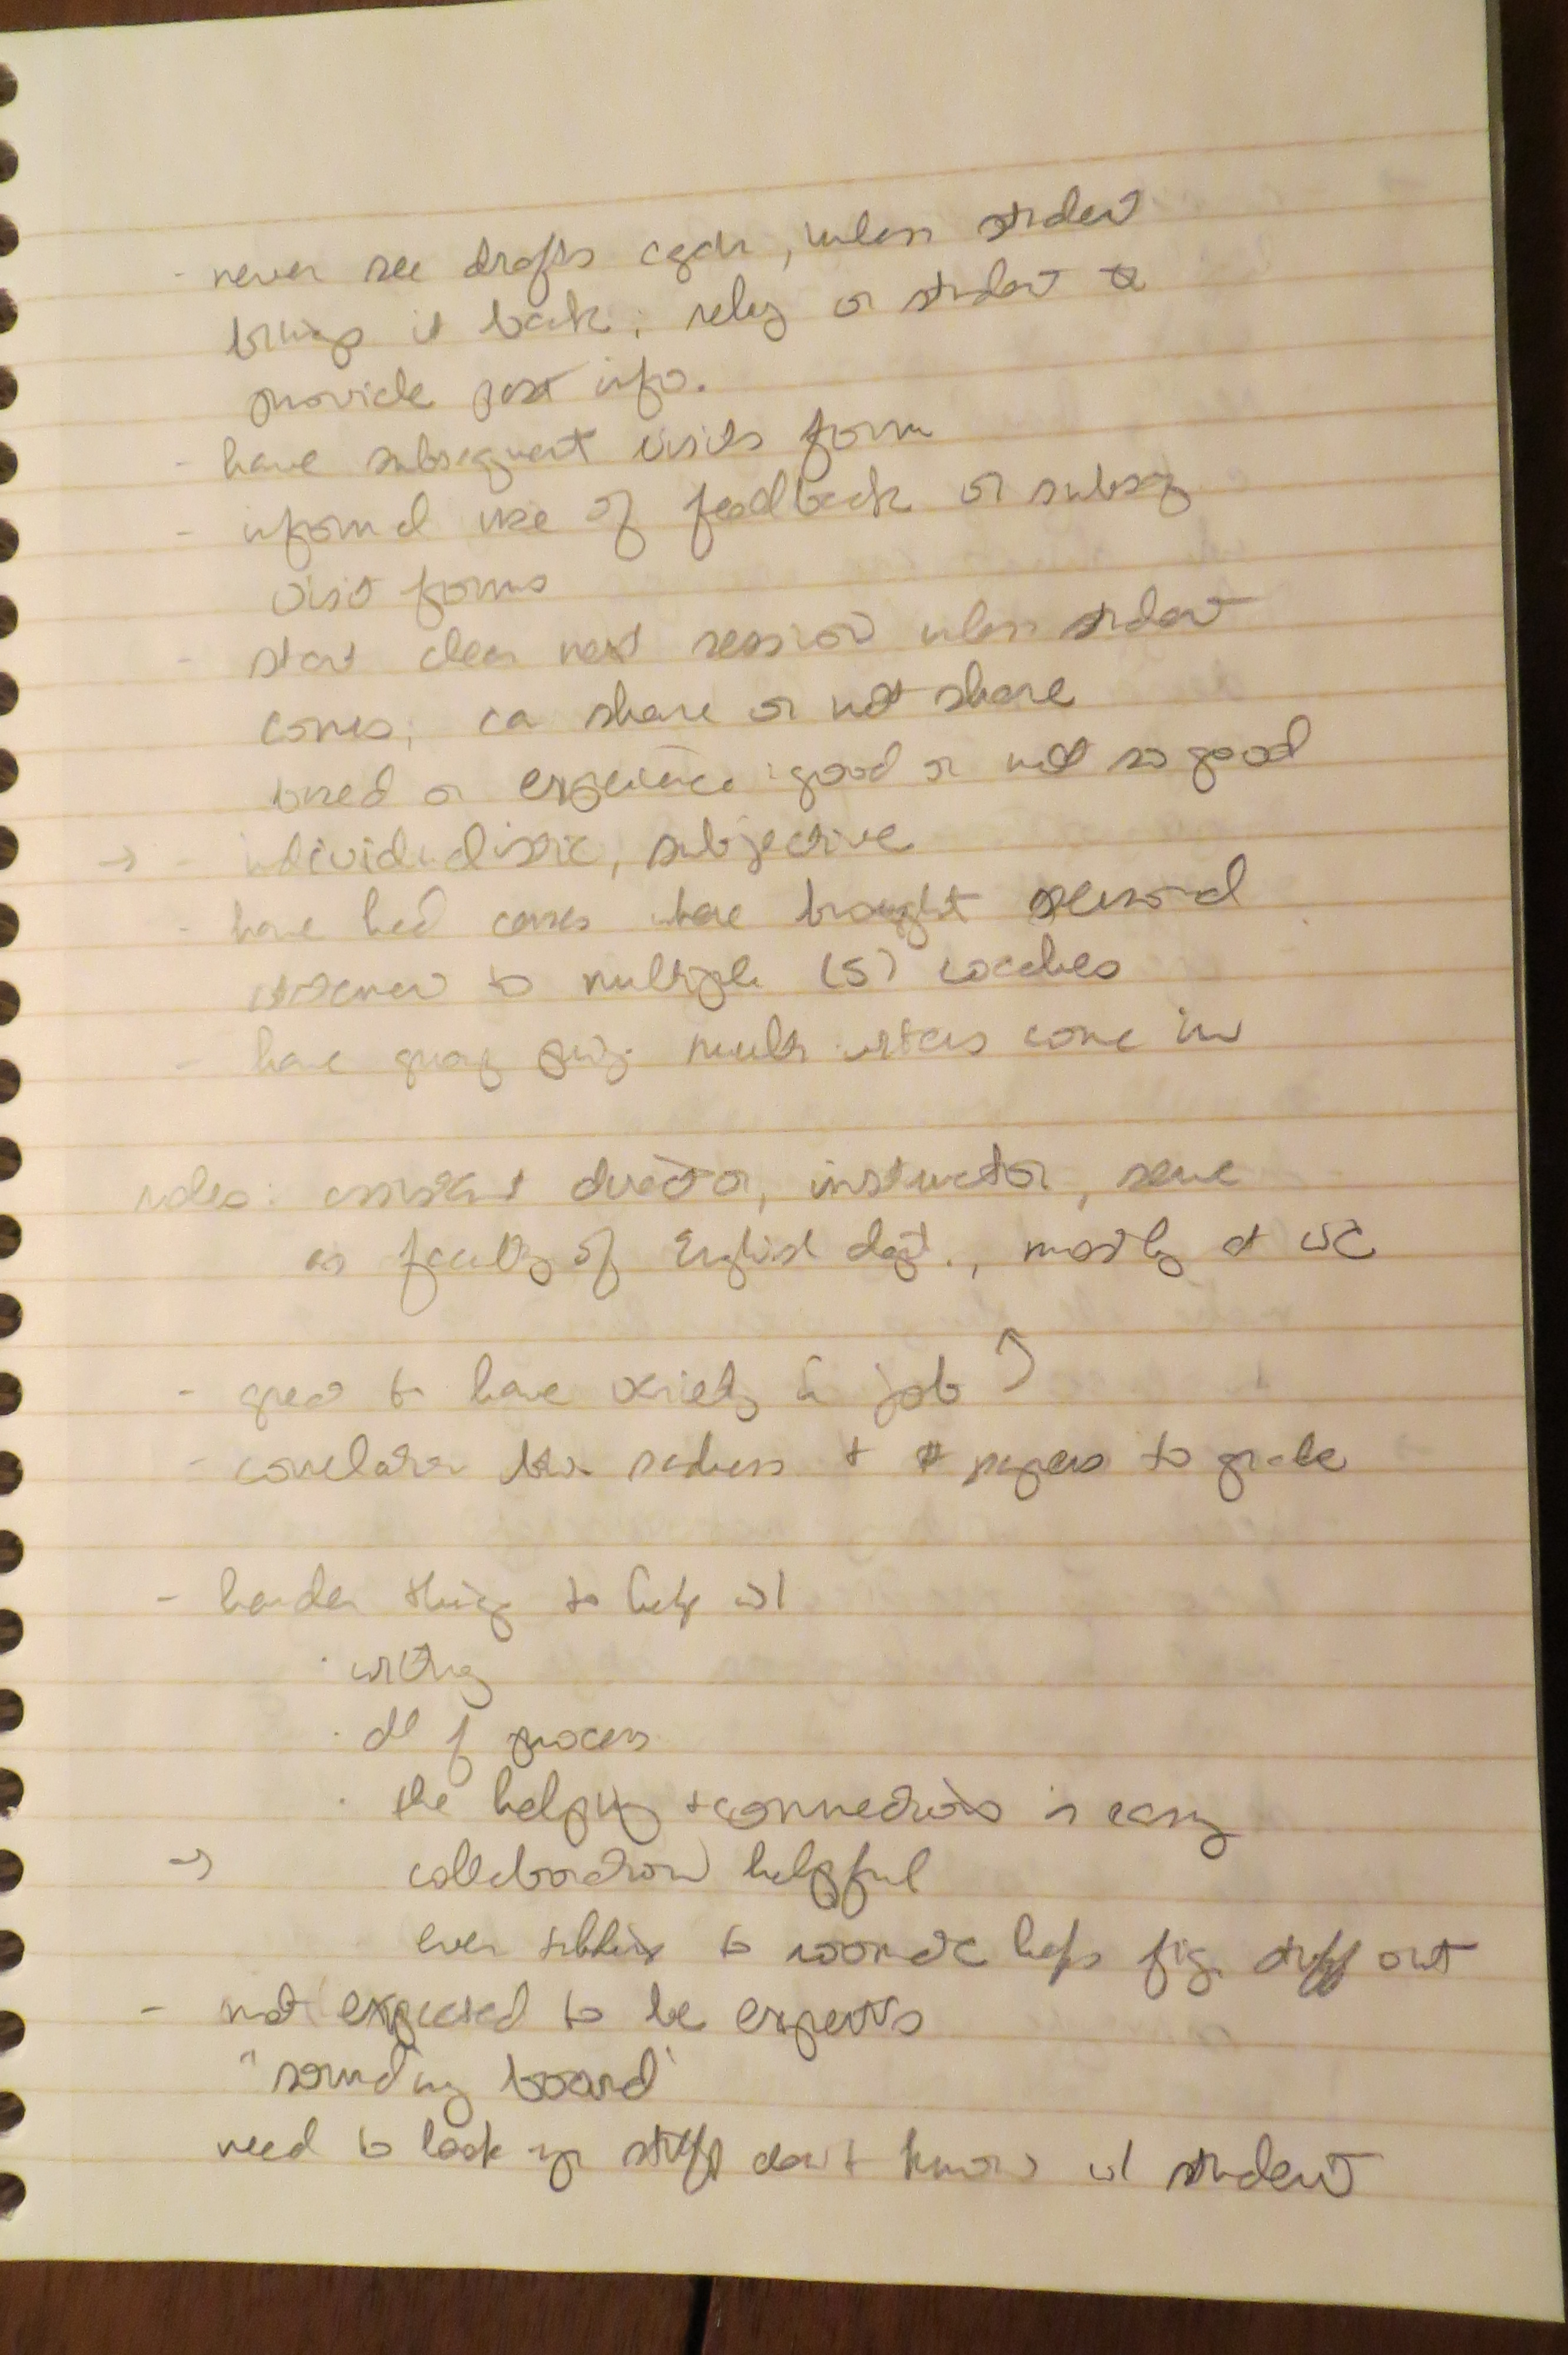
\includegraphics[width=0.75\linewidth]{RAZ_raw_notes5}
  \caption{}
  \label{fig:rn5}
  \end{figure}
  \begin{figure}[H]
  \centering
  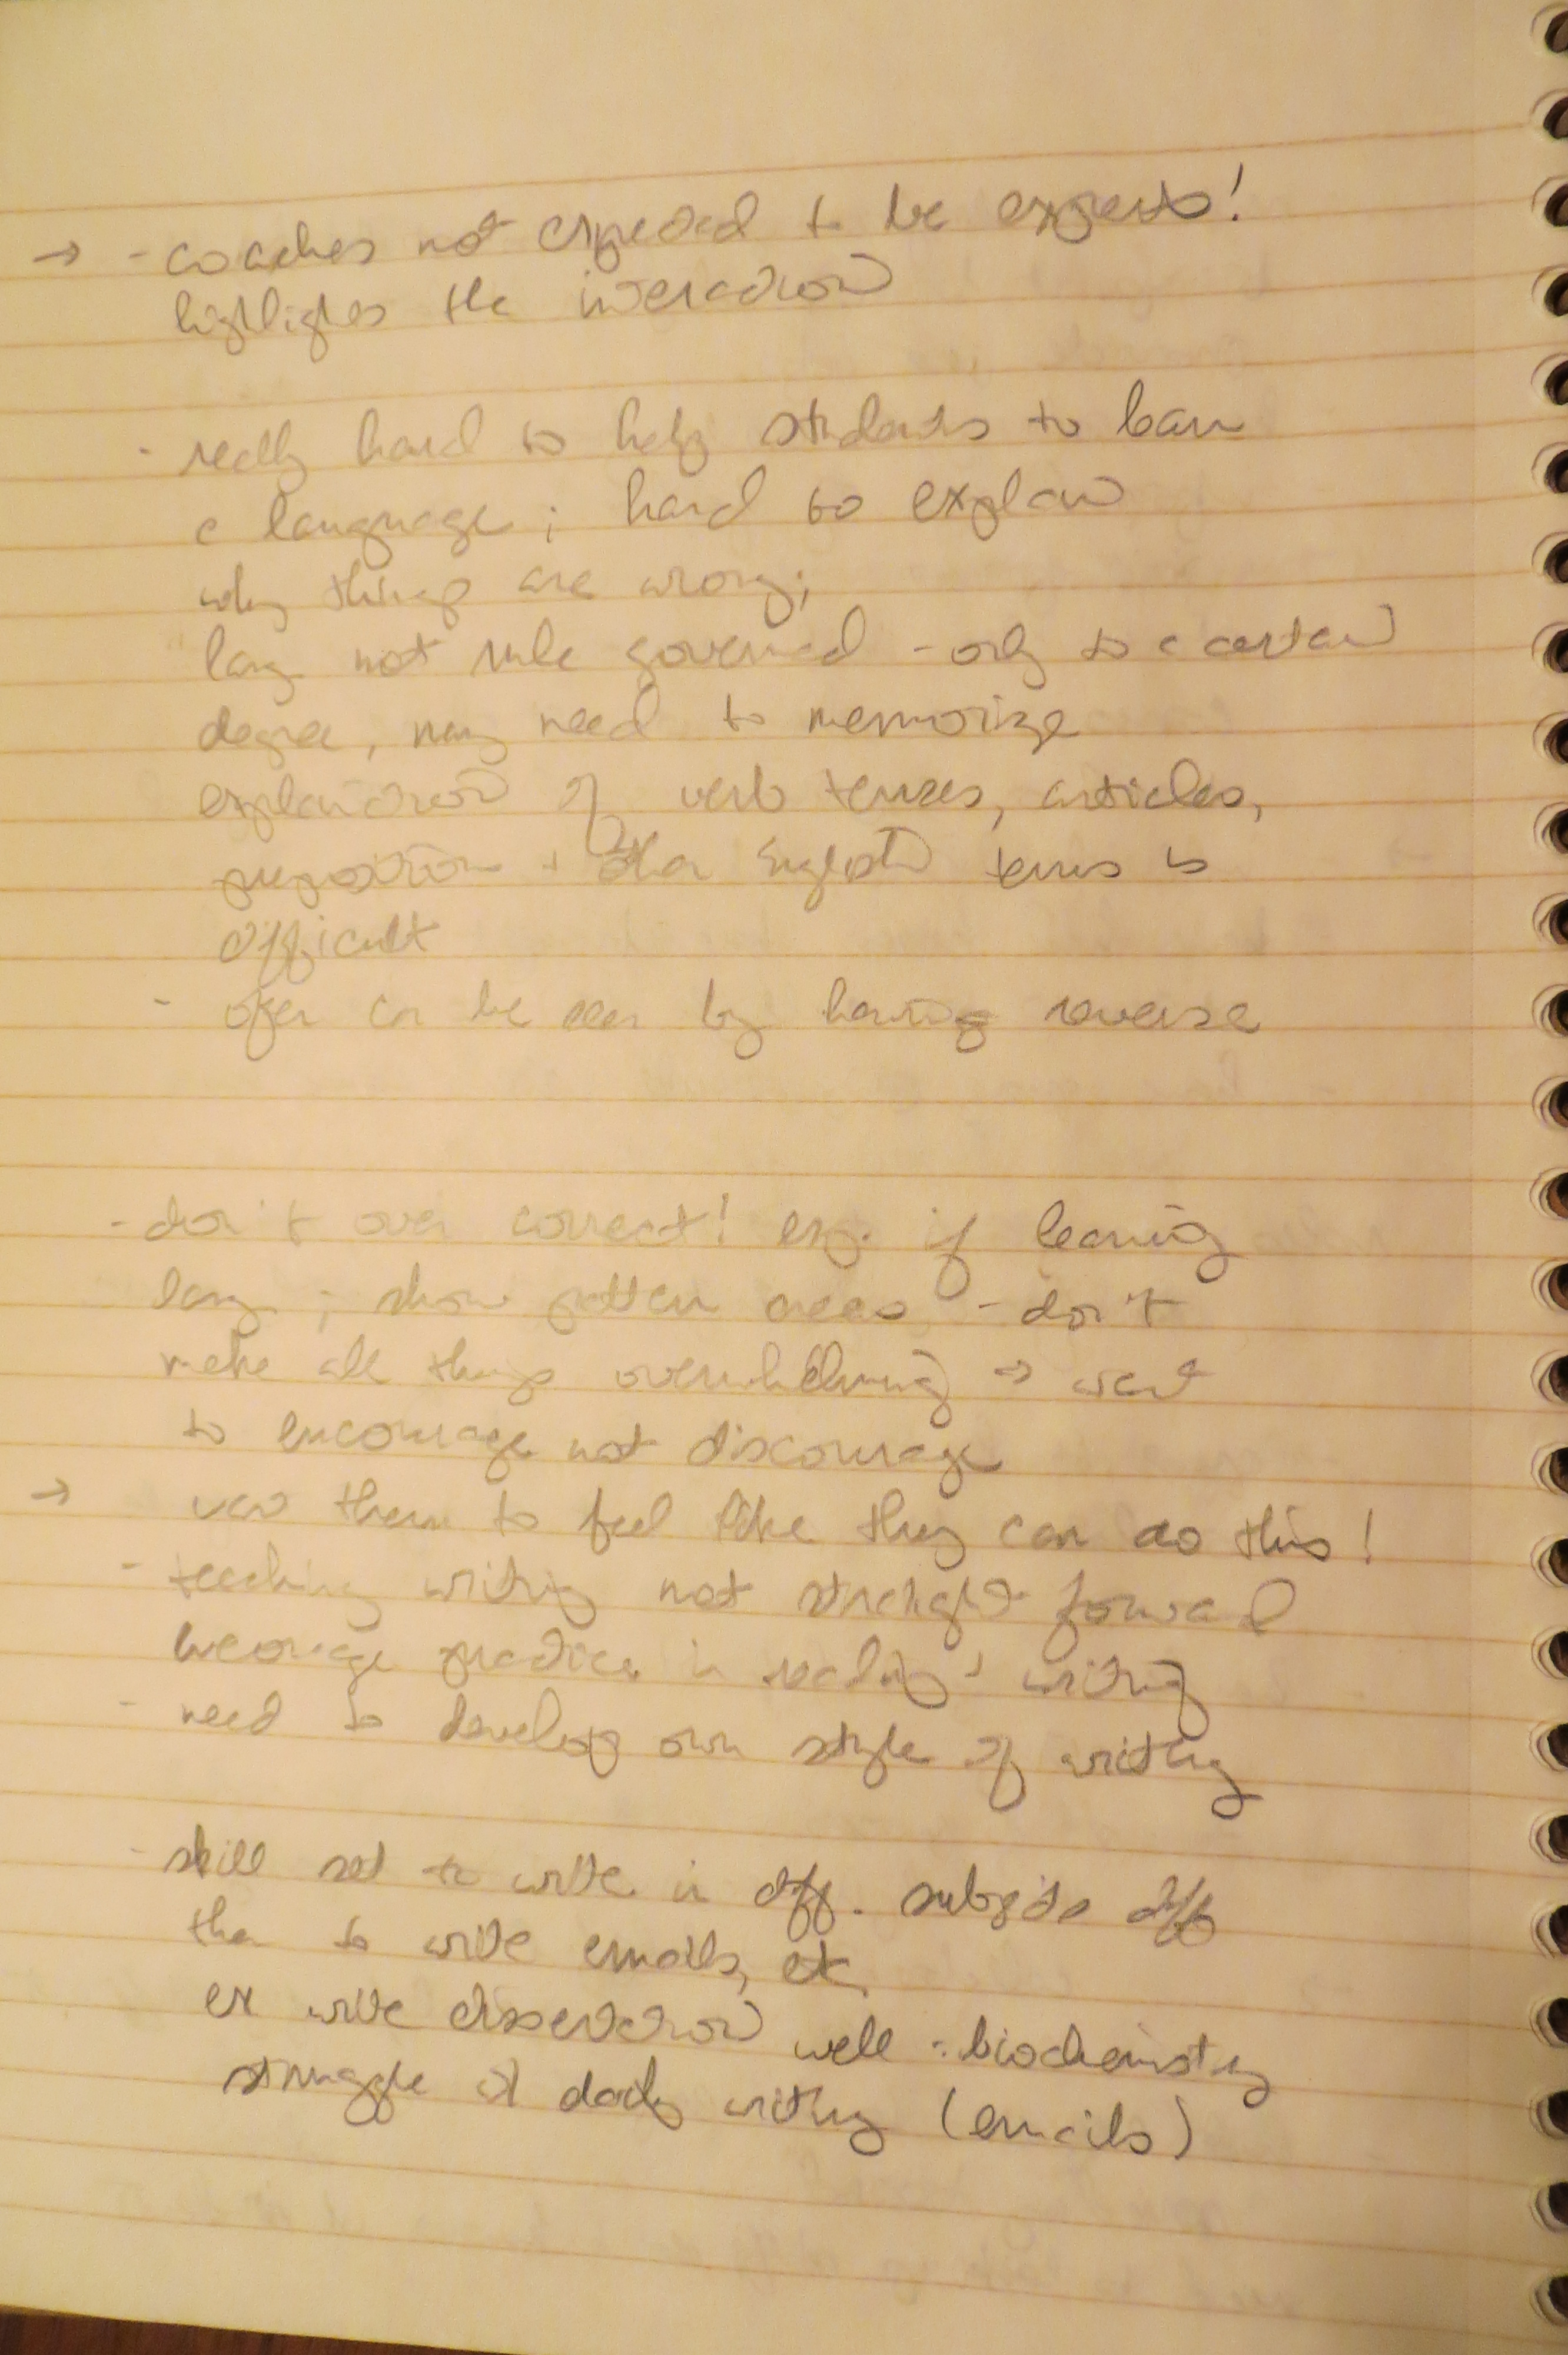
\includegraphics[width=0.75\linewidth]{RAZ_raw_notes6}
  \caption{}
  \label{fig:rn6}
  \end{figure}
  \begin{figure}[H]
  \centering
  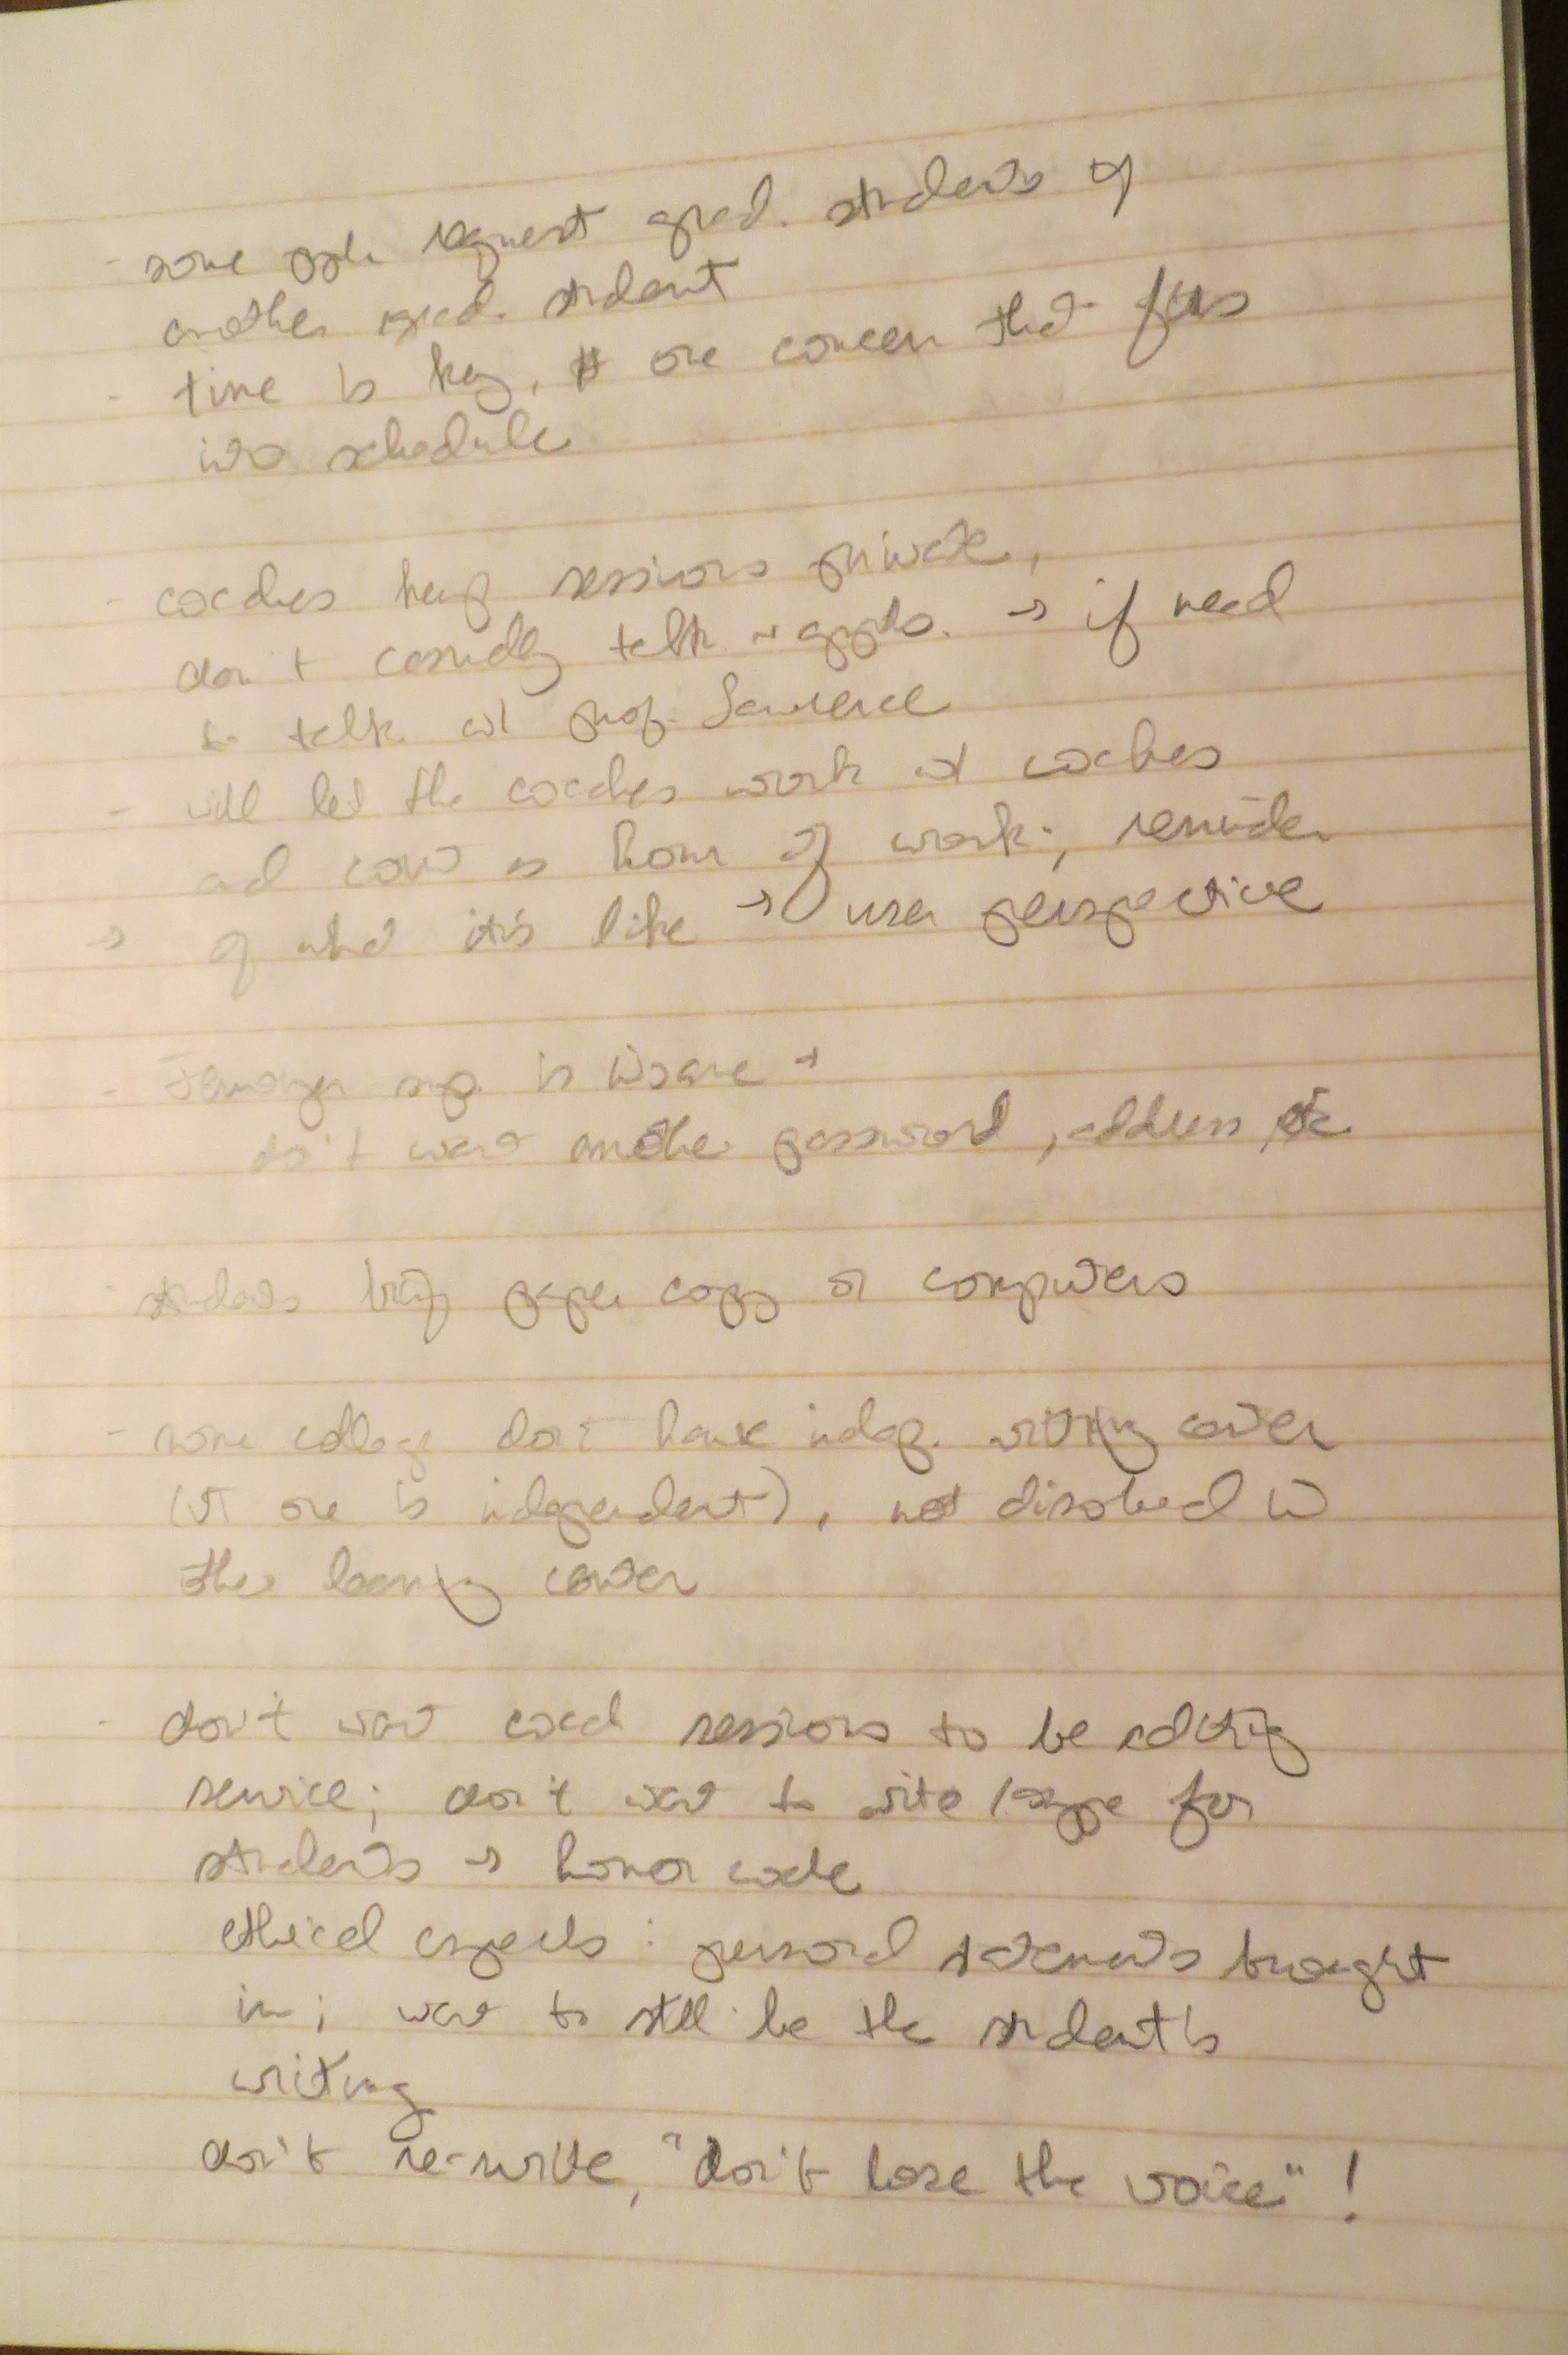
\includegraphics[width=0.75\linewidth]{RAZ_raw_notes7}
  \caption{}
  \label{fig:rn7}
  \end{figure}
  \begin{figure}[H]
  \centering
  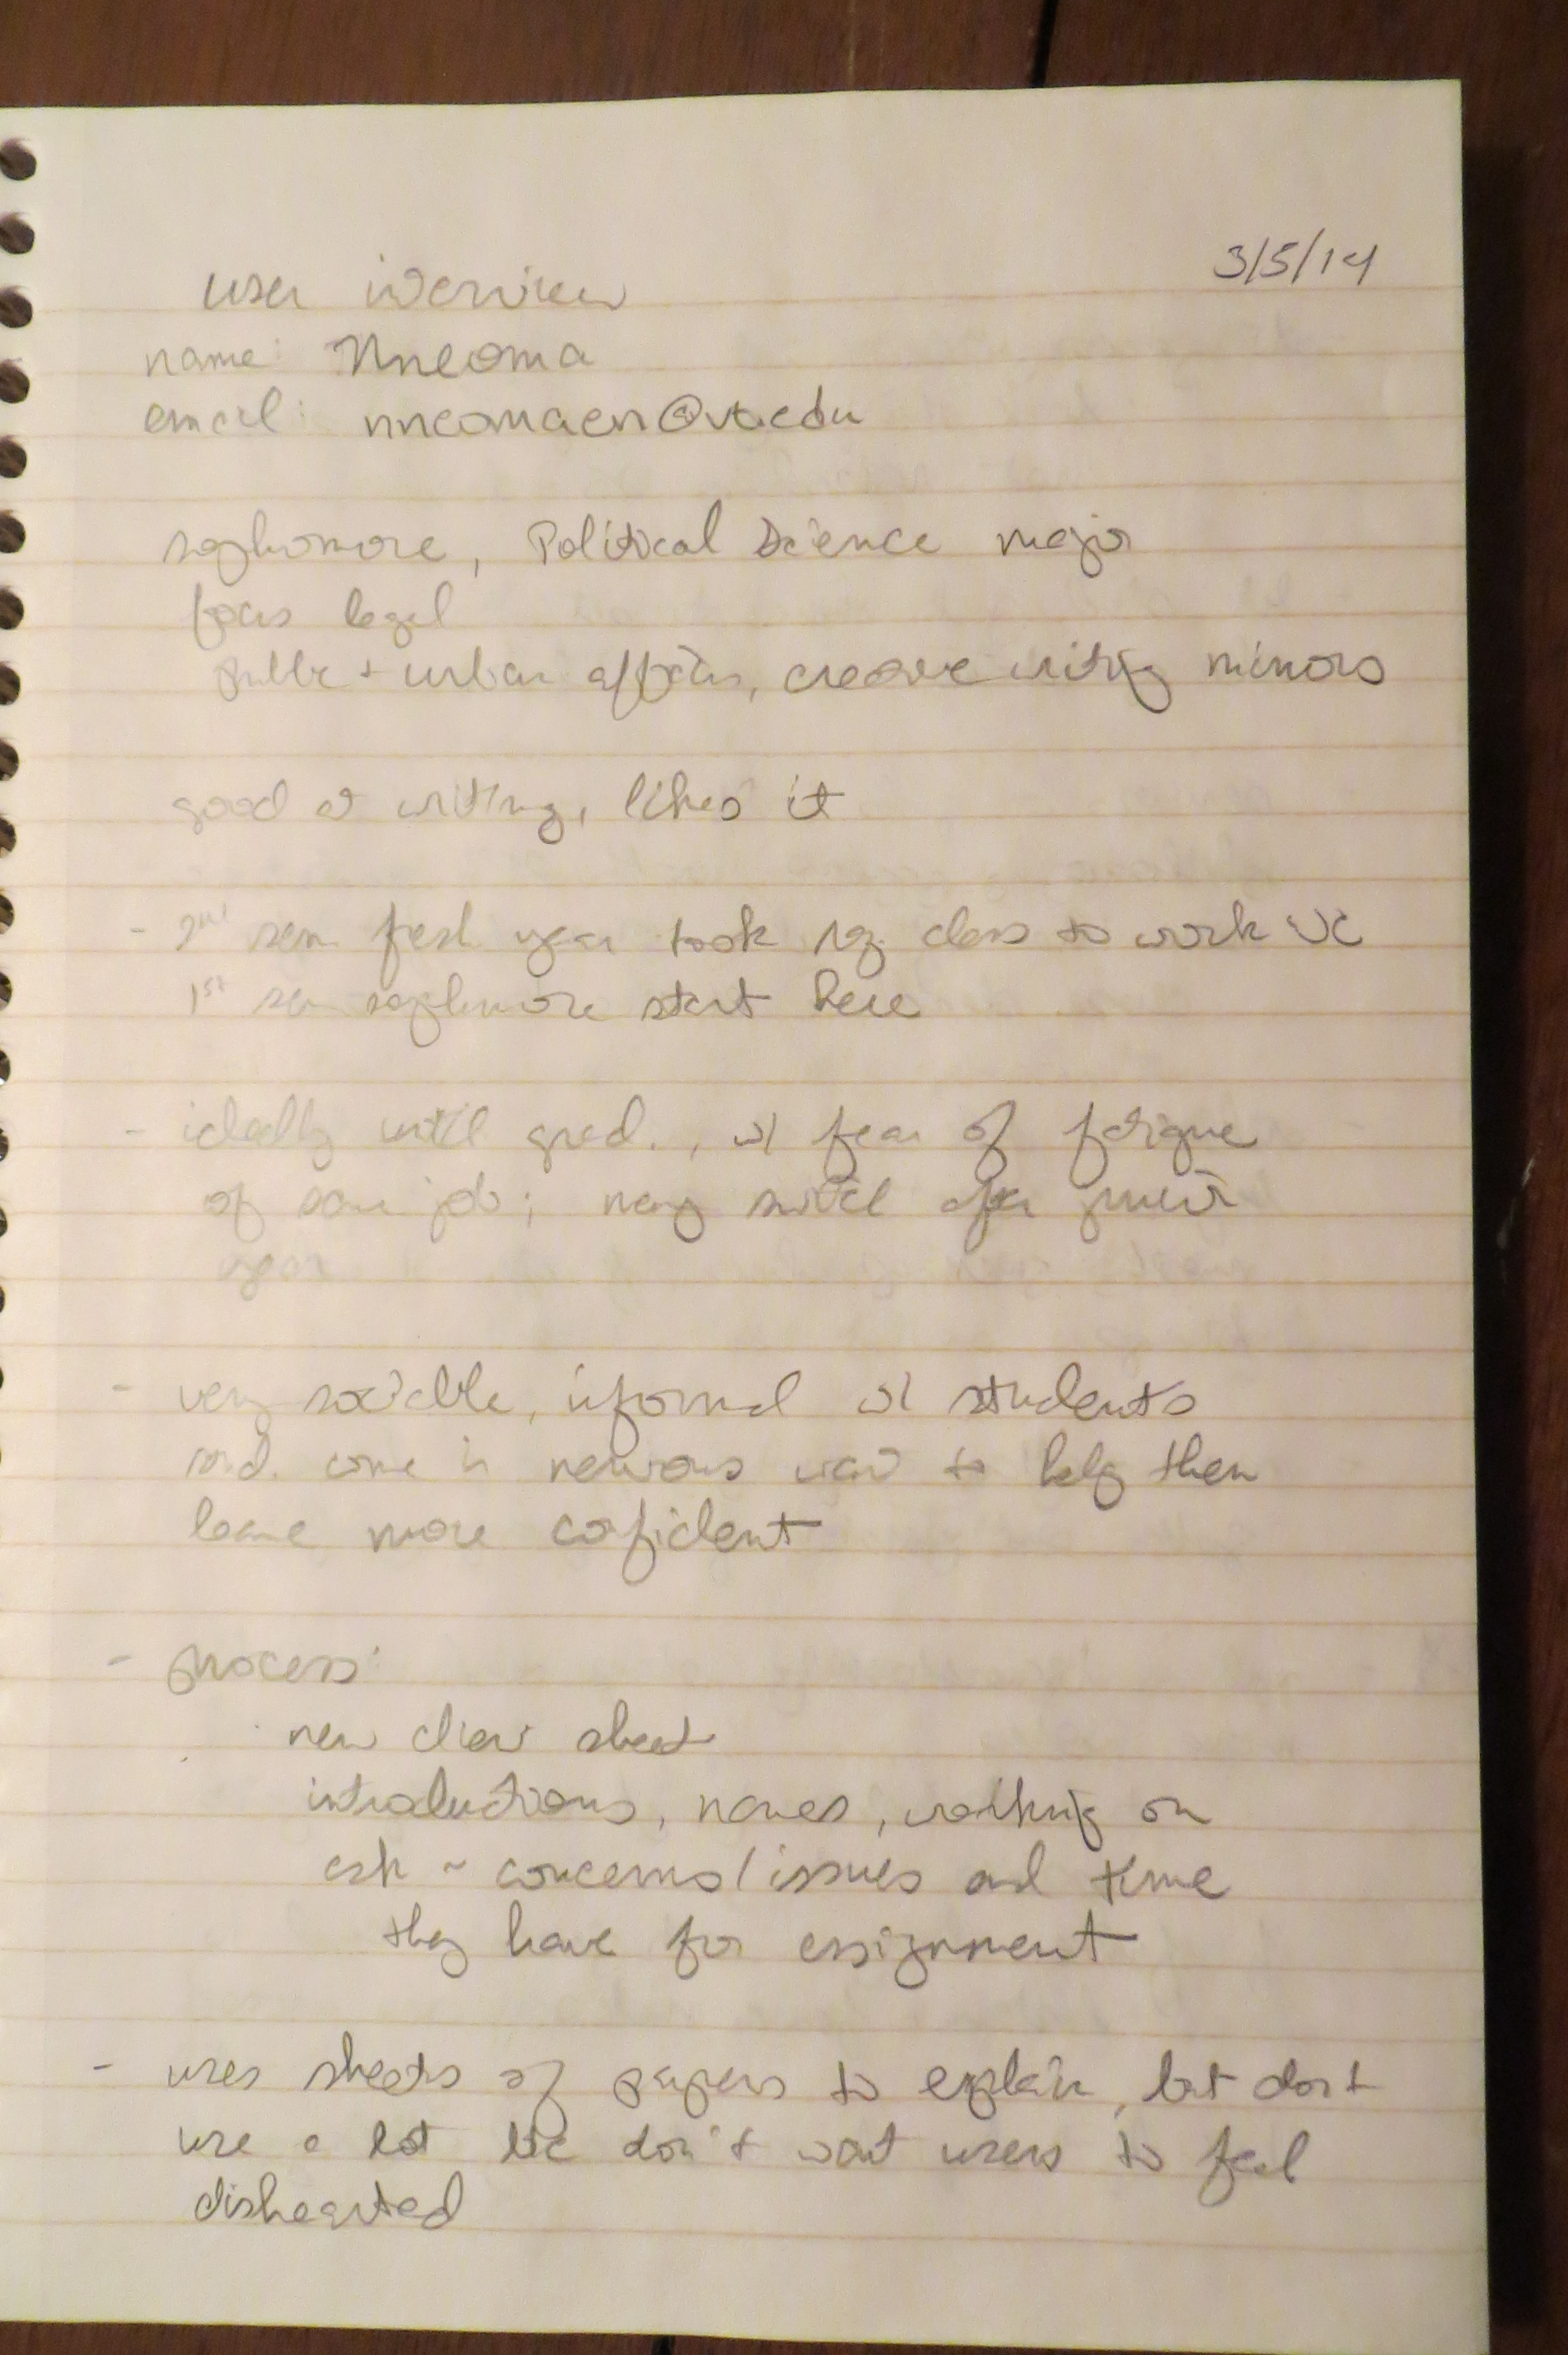
\includegraphics[width=0.75\linewidth]{RAZ_raw_notes8}
  \caption{}
  \label{fig:rn8}
  \end{figure}
  \begin{figure}[H]
  \centering
  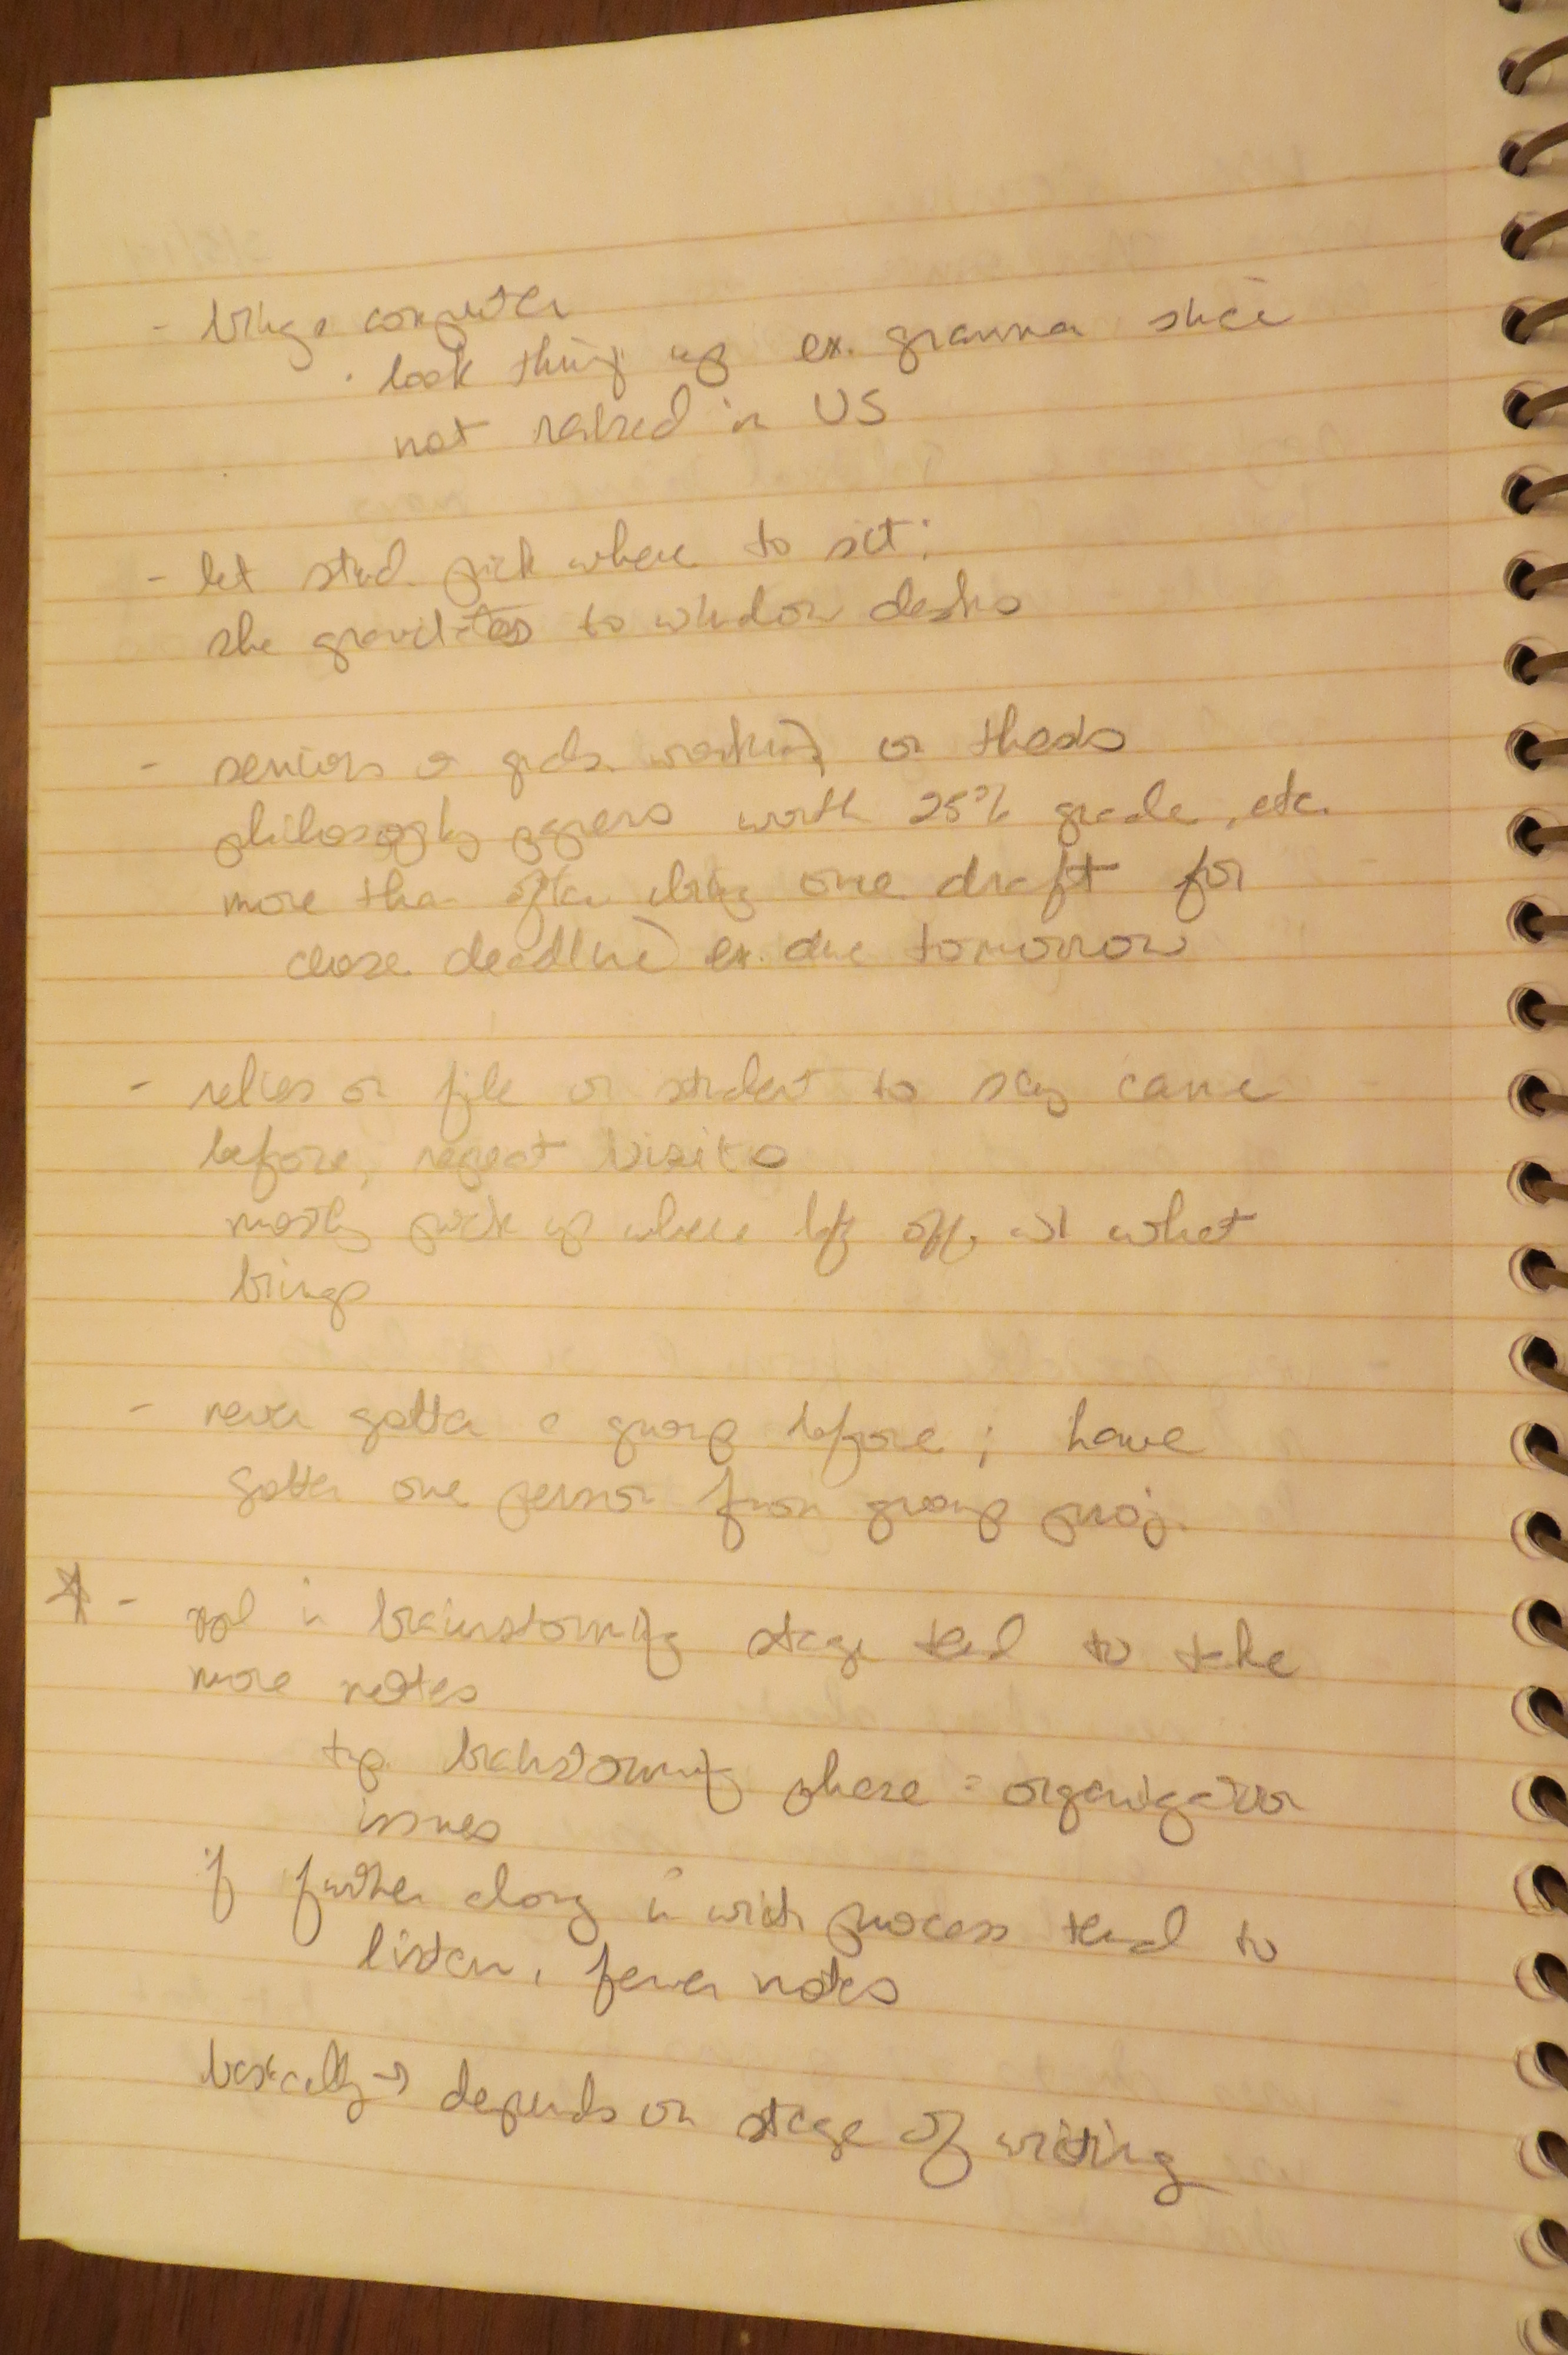
\includegraphics[width=0.75\linewidth]{RAZ_raw_notes9}
  \caption{}
  \label{fig:rn9}
  \end{figure}
  \begin{figure}[H]
  \centering
  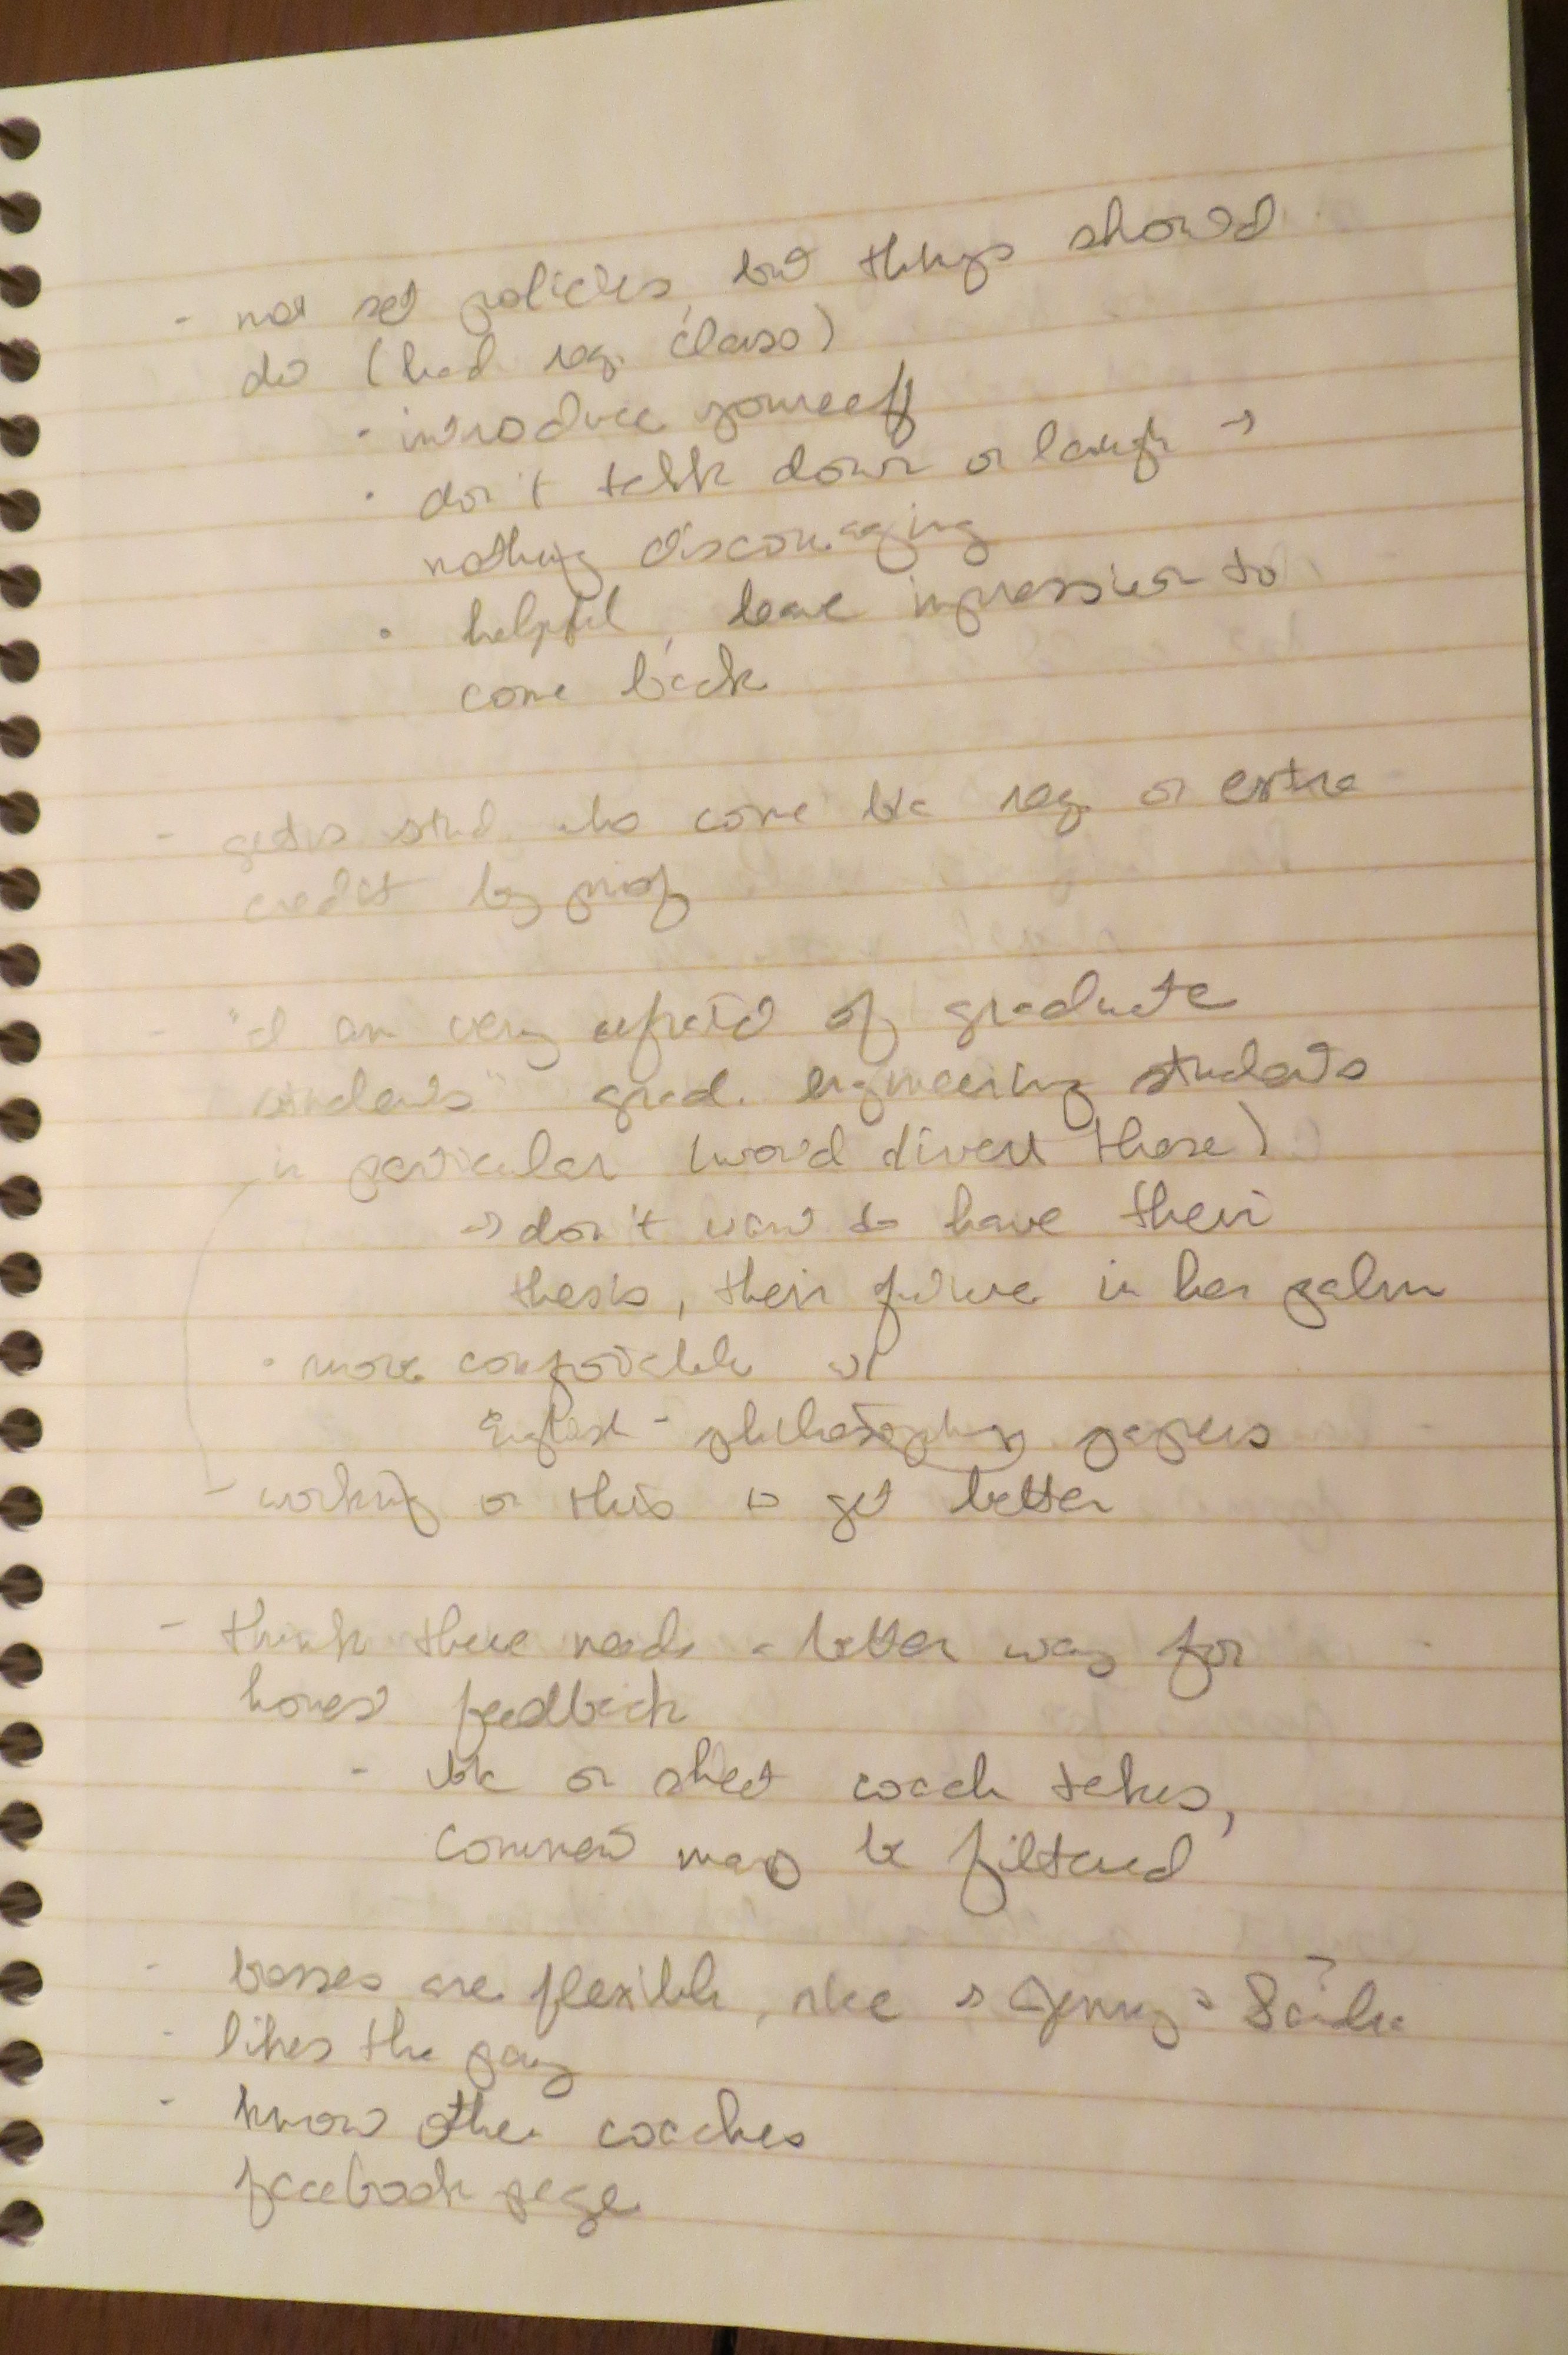
\includegraphics[width=0.75\linewidth]{RAZ_raw_notes10}
  \caption{}
  \label{fig:rn10}
  \end{figure}
  \begin{figure}[H]
  \centering
  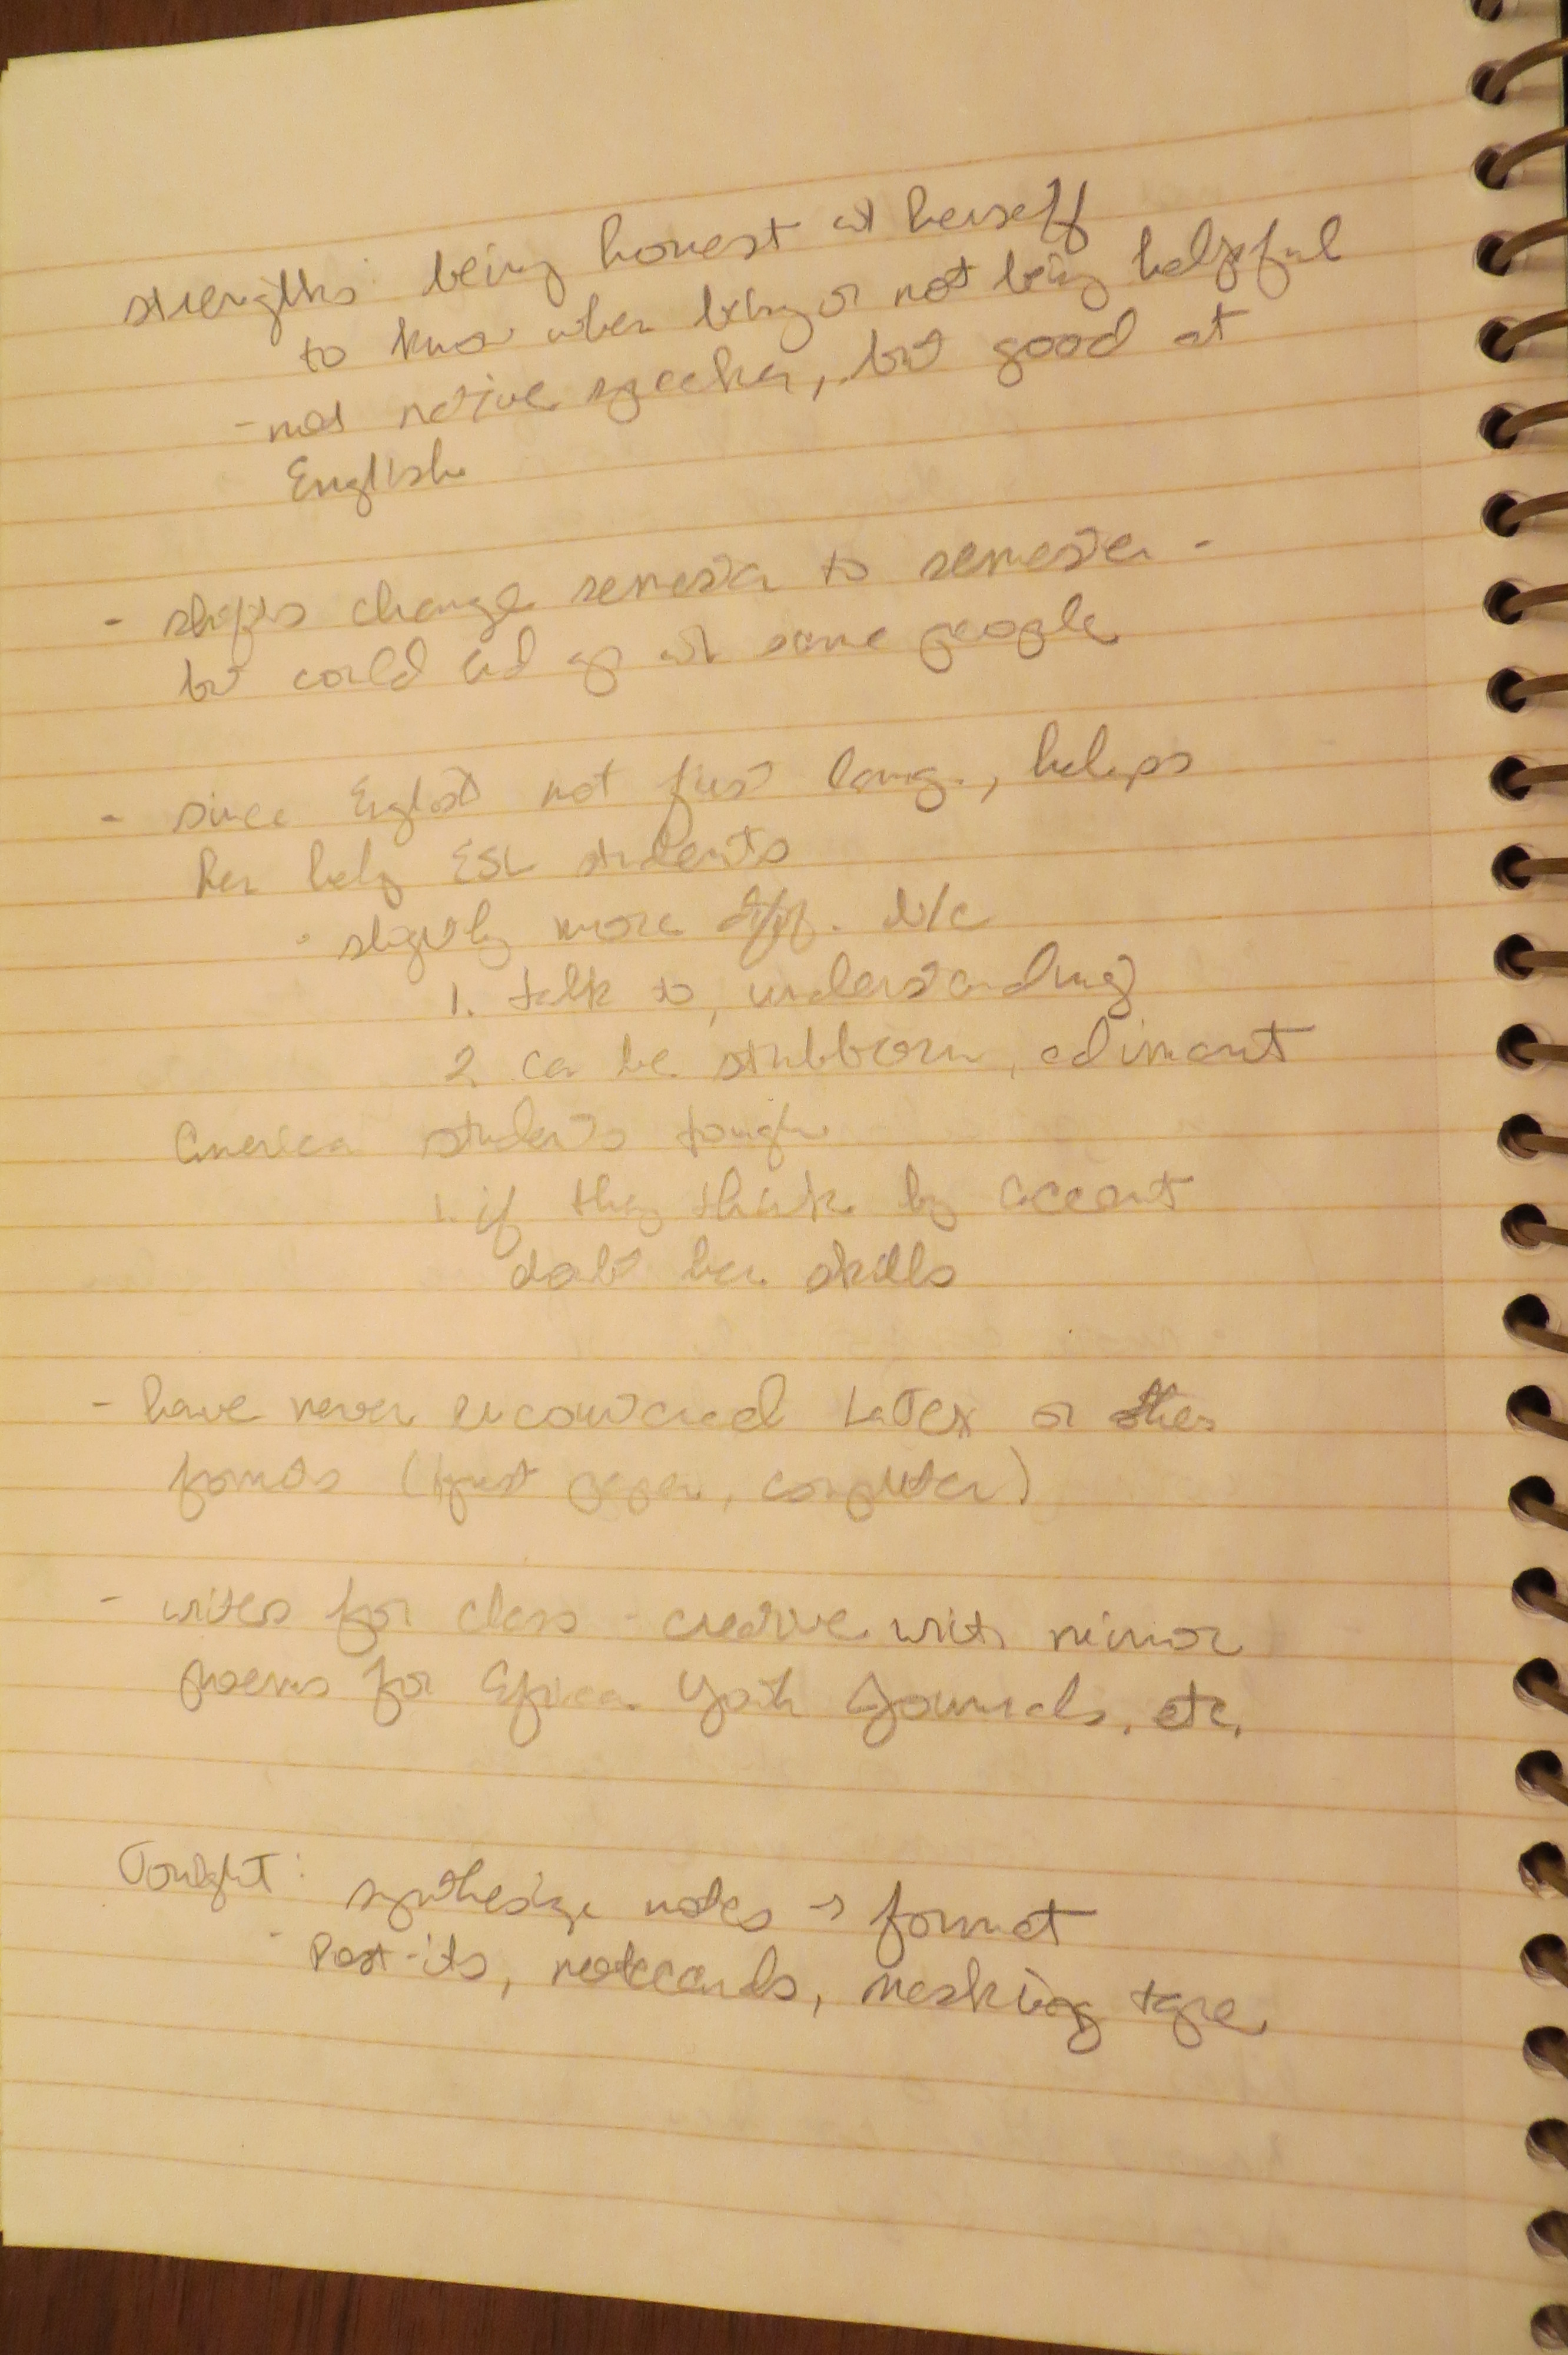
\includegraphics[width=0.75\linewidth]{RAZ_raw_notes11}
  \caption{}
  \label{fig:rn11}
  \end{figure}
  \begin{figure}[H]
  \centering
  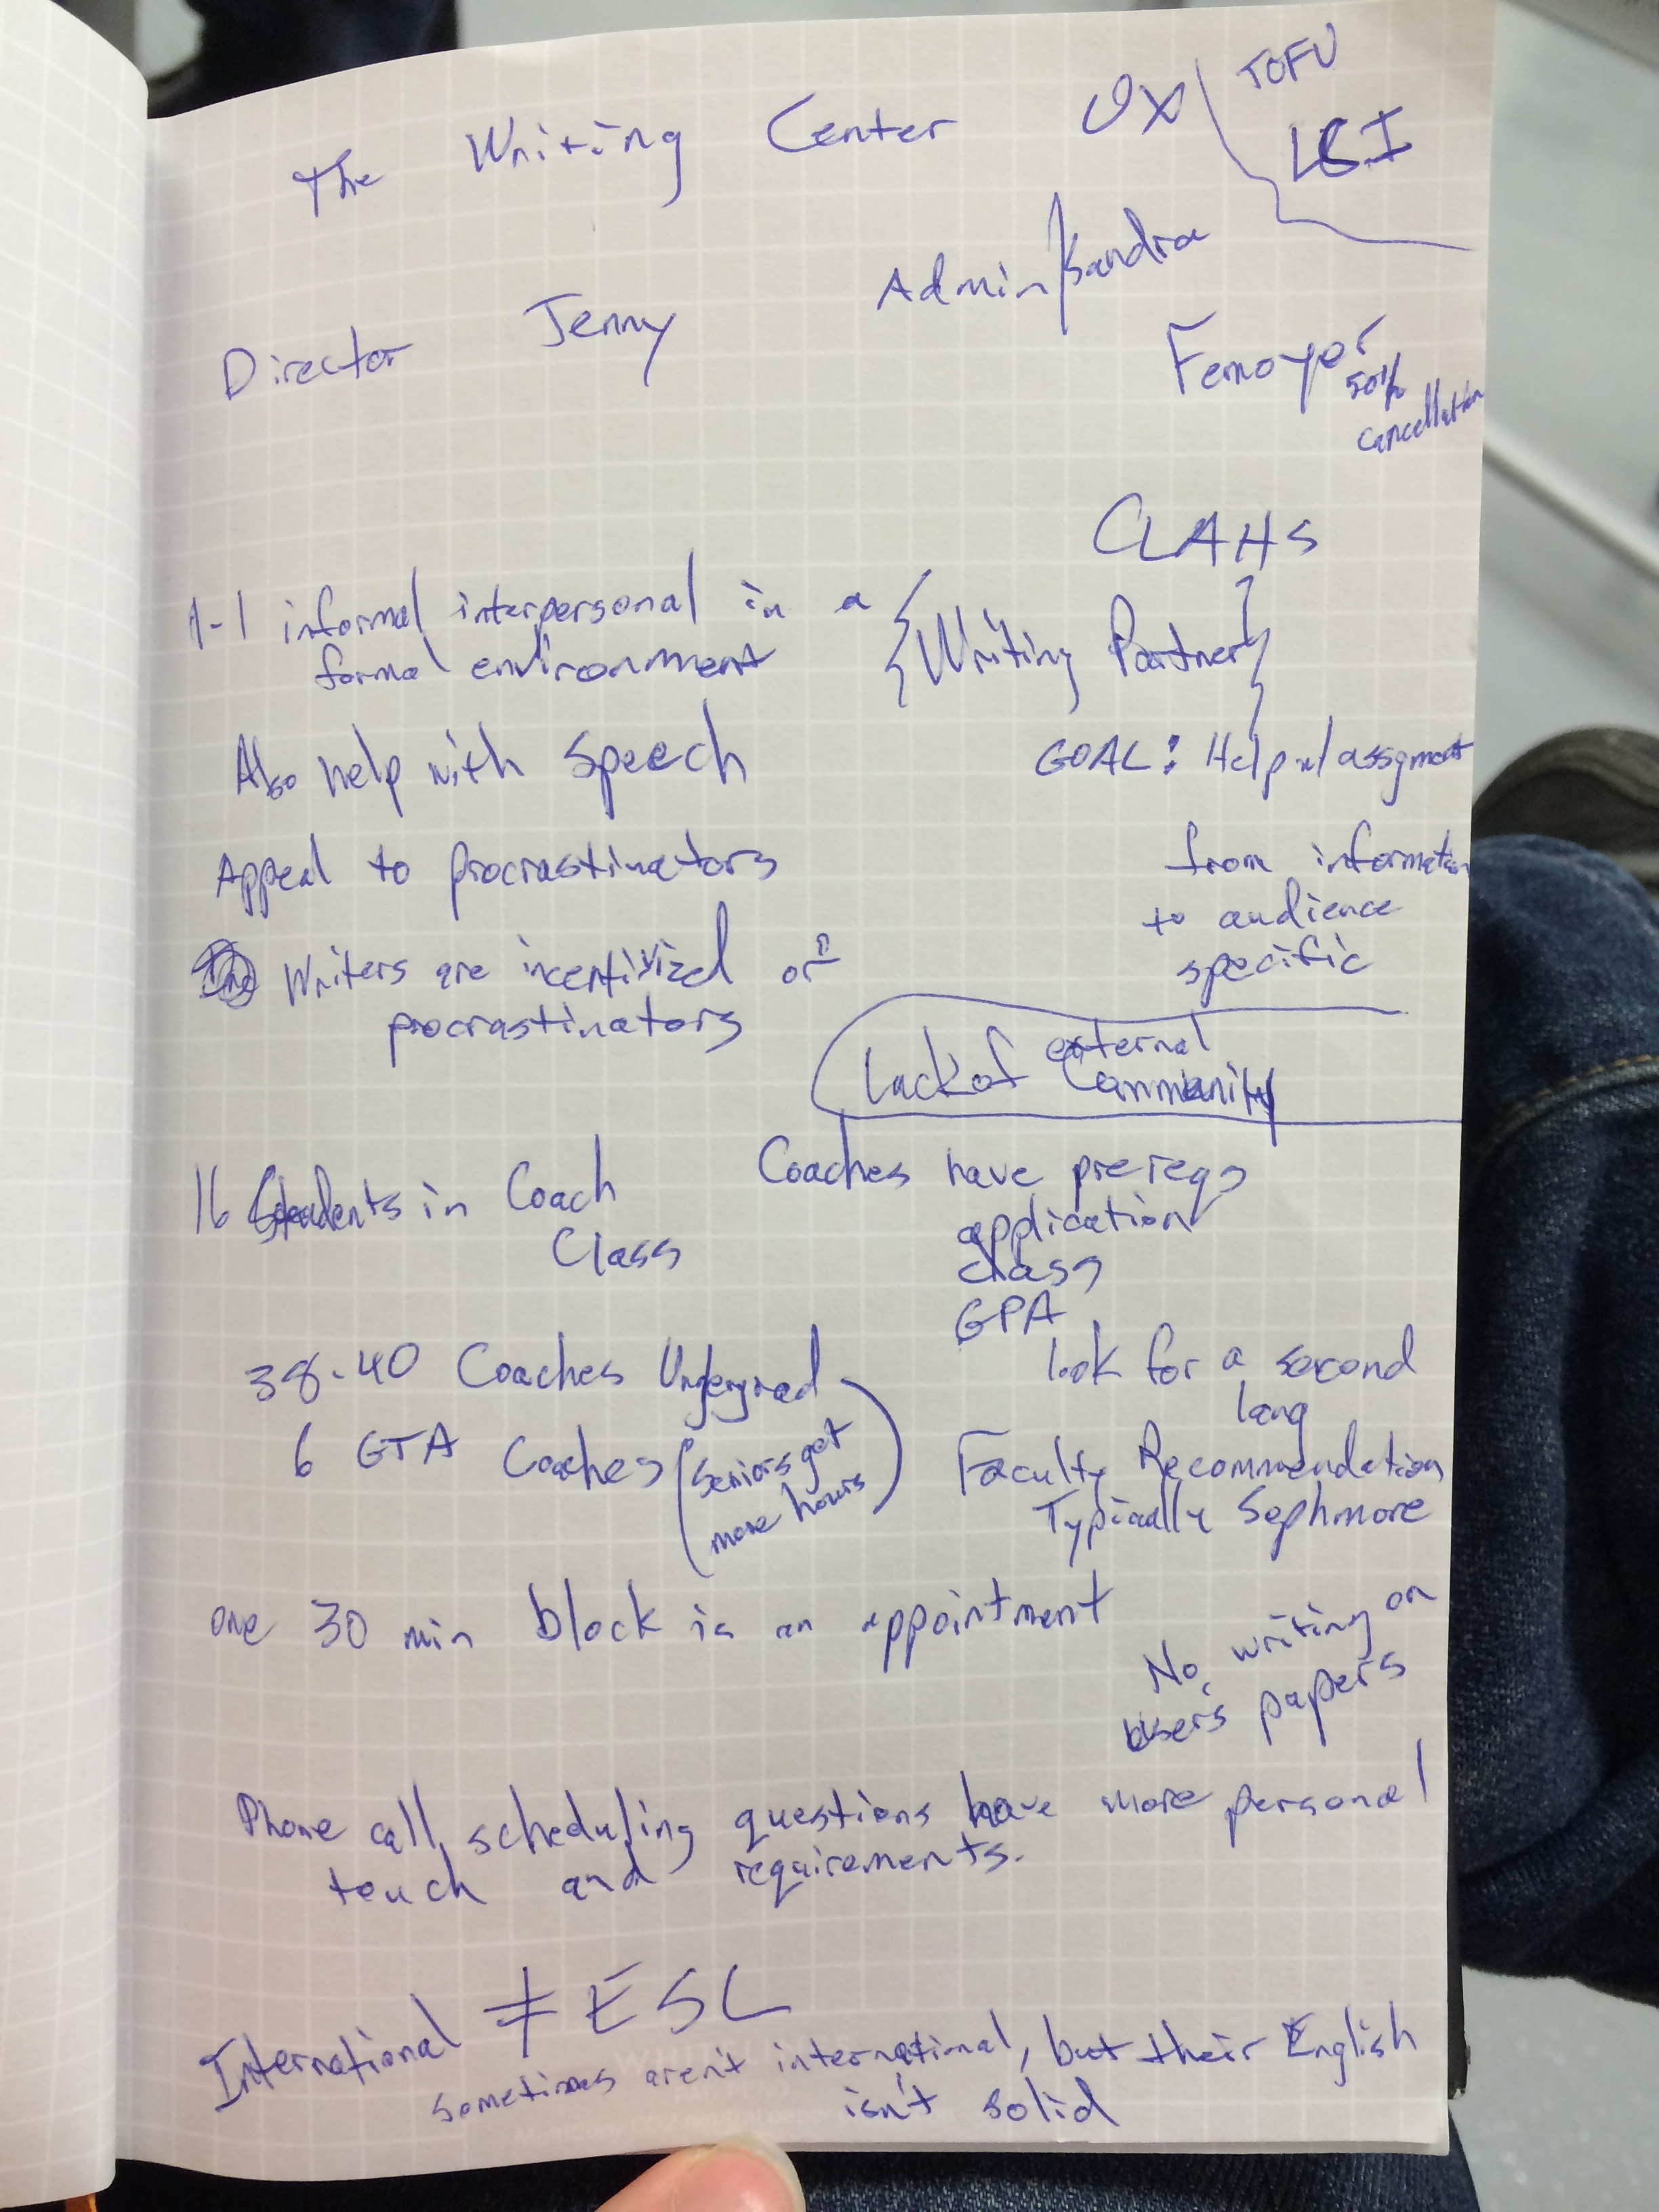
\includegraphics[width=0.75\linewidth]{special-raw-notes}
  \caption{}
  \label{fig:rn12}
  \end{figure}

  \subsection*{Work Activity Notes}

  Interviewee: Professor Jennifer Lawrence 
  Email: \href{mailto:jlwrnc@vt.edu}{jlwrnc@vt.edu}
  Work Roles: Assistant Director of the Writing Center (WC) at Virginia Tech, Coach
  ID: ADIR

  \begin{itemize} \itemsep1pt \parskip0pt \parsep0pt
    \item Management of the WC staff is divided; The Director of the WC manages the graduate coaches (TAs), while the Assistant Director of the WC manages the undergraduate coaches.
    \item Most of the funding for the WC comes from the English department.
    \item Concerning the atmosphere, the staff of the WC tries to keep it professional, but informal in a lot of ways.  The WC sessions are one on one.  Introductions are on a first name basis. 
    \item The WC helps students wherever they are in the writing process, from starting and brainstorming to written or more complete drafts.
    \item Writing Center coaches should not write on or edit the client papers.
    \item The client is in control of any edits.
    \item The WC coaches often have clients read their papers or written works aloud to help find mistakes.
    \item The WC coaches help the client take their papers from a writer focus to an audience focus, shifting the focus from the writer to the audience.
    \item Next semester, the WC will be extending their hours.  The WC will continue to hold drop-in sessions and sessions by appointment.
    \item Students interested in becoming writing center coaches must fill out an application and be accepted in order to enroll in English 3744, the required course for coaches.  About 16 get enrolled in that, and new coaches are hired from that pool.
    \item There is no official cut-off GPA for students applying to be a WC coach.
    \item For hiring coaches, WC tries for honors students and double majors.
    \item WC looks to hire students who are double majoring, with one major being a language or majors that span different areas, ie. Computer Science and English. 
    A lot of the WC coaches are English majors.
    \item Typically, a coach works for two years at the writing center.  The high turnover rate was mostly contributed to students graduating and studying abroad.
    \item There are about 6 GTA WC coaches.  These coaches typically want experience in teaching.
    \item There are about 38 current coaches.
    \item WC typically hires coaches after their sophomore year (but there are exceptions).
    \item Full time work at WC for graduate coaches is 12 hours/week, 6 hours/week if coaches are in composition class.  Undergraduate coaches are typically offered 6 hours/week.
    \item Hours, Sunday hours in particular, are a double edged sword; The WC has lot of Sunday sessions because of client procrastination, extra credit offers by professors, or assignment extensions offered by professors.
    \item The WC sessions are scheduled in 30 minute blocks of time, or two 30 minute blocks of time scheduled back to back.  The WC tries to limit a single client to 1 hour per day.  However, decisions are made on a case by case basis.
    \item The WC tries to be accommodating and flexible in scheduling sessions.
    \item Quite often, there are six sessions simultaneously going on.
    \item WC Coaches are to give the feedback the client requests.  Coaches  are expected to give their perspective, but no to force it if the client disagrees.  Coaches are there to help, not lecture.
    \item WC does not use online scheduling.  WC has reason to believe that clients are more likely to show up when making the appointment over the phone.  WC bases this off of the about 50% appointment cancellation rate for the Student Success Center at Femoyer Hall.
    \item WC likes the personal effect of phone call appointment scheduling.
    \item A running tally of appointments is kept each day in a Microsoft Excel spreadsheet.
    \item Client visit/visit feedback sheets are paper forms.
    \item WC helps with other things that are not writing assignments, such as personal statements, resumes, and cover letters.
    \item Most of the time, clients come in with a rough draft.
    \item The majority of clients are English majors and graduate students.
    \item Coach comments are either verbal or on pad of paper for notes, available if needed.
    \item Clients infrequently email concerns to the WC.  Most feedback given on client visit form.
    \item Coaches are sometimes writing partners, who will help a client throughout a semester.
    \item Clients can requests weekly appointments with a coach.
    \item WC holds a community WC at Blacksburg library, but not many clients.  Community clients could come to Virginia Tech location, but this is not advertised. 
    \item WC helps with any communication, not just written papers.  This includes writing and reading.
    \item The one on one session is intended to create a personal atmosphere with learning on both the coach and client side.
    \item WC coaches never see client drafts unless the client brings them.  Coaches rely on client to bring in any relevant or past information.
    \item WC has a subsequent visit as well as first time visit form for clients.  These are kept in a file cabinet.
    \item WC has an informal use of the visit/feedback and subsequent visit forms.
  \end{itemize}
  
  ID: C1
  \begin{itemize}
    \item The sessions all start from a clean slate unless the client bring past information.  Client can choose what information is shared or not shared, which may be based on if has a good or bad experience in a session.
    \item WC coach is a “sounding board,” not expected to be an expert.
    \item WC coaches are encouraged to look up things they do not know, even in front of the client.
    \item WC coaches can find it hard to explain why things are wrong when teaching a client to learn English.  Languages are only rule governed to a certain degree, which means a learner will need to memorize some things.
    \item As a WC coach, explaining verb tenses, articles, prepositions, and other English terms is difficult.
    \item WC coaches should not over correct.  They are to show a pattern area of corrections, not overwhelm the client.  WC coaches want to encourage not discourage.
    \item WC coaches want clients to develop their own style of writing.
    \item Skill sets for writing are different across different subjects and different types of writing (i.e. technical papers vs. emails/everyday communications).
    \item Graduate student clients tend to request graduate student coaches.
    \item Time is key; the number one concern when scheduling is if it can fit into the clients schedule.
    \item Coaches are to keep sessions private, maintain client confidence and trust.
    \item Coaches can work with other coaches and count this as their WC hours.  From this, coaches can gain and be reminded of a client perspective.
    \item Clients bring in writings on paper or computer.
    \item WC is not intended to be providing an editing service.
    \item Want to uphold ethical standards.  Want writings brought in to still be the client’s writing, not the coach’s.  WC want the clients to maintain their voice in their writings.  Don’t lose the voice!
  \end{itemize}
  
    Interviewee: Nneoma Enyi Nwankwo
    Email: nneomaen@vt.edu
    Work Role: Writing Center Coach (VT sophomore, Political Science major, public and urban affairs and creative writing minors)
    ID: C2
    
  \begin{itemize}
    \item Coach can ideally work at WC until graduate.
    \item WC coach maintains sociable, informal conversation with client. 
    \item WC coaches want to have clients leave with more confidence than they came in with.
    \item WC coach has a general process:
    \begin{enumerate}
    \item	Give client new visit form to fill out
    \item	Makes introductions, first name basis
    \item	Asks what client is working on
    \item	Asks what concerns about the work the client has
    \item	Ask what the time constraints are (i.e. when the assignment is due)
    \end{enumerate}
    \item Uses sheets of paper to explain, but does not use a lot because doesn’t want client to feel disheartened.
    \item Coach brings computer to look things up if needed. 
    \item Coach lets the clients pick where to sit.  Coach prefers to sit at one of the desks by the windows.
    \item Clients most often bring one draft of assignment and close to deadline. 
    \item Clients are often seniors or graduate students working on thesis papers.  Clients are also often philosophy students working on papers worth 25% of their grade.
    \item Coach has never gotten a group of clients for one session, but has had a single client from a group project team.
    \item Clients in brainstorming stage tend to take more notes than clients who are further along in the writing process. 
    \item Clients further along in the writing process tend to mostly listen, taking very few notes if any.
    \item Typically, clients in the brainstorming stage tend to have organization issues. 
    \item Coach help depends on the stage of the writing process the client is at.
    \item Guidelines coaches follow include introducing themselves, being helpful in general, leaving an impression that makes the client want to come back, and not talking down, laughing, or doing anything that may discourage the client.
    \item Coach is afraid of graduate students, specifically graduate engineering students.  Doesn’t want to have their thesis, their future, in the coach’s palms.  Coach is working to get better at helping these clients.
    \item Coach is most comfortable with English and Philosophy papers. 
    \item Coach thinks there needs to be a better feedback system.  Coach thinks that since the feedback system is on the visit form where the coach can see it, it gets returned to the coach at the end of the session, that the comments may be filtered.
    \item Coach thinks bosses are flexible and nice.
    \item Coach knows other coaches, but mostly those who have been working the same hours.
    \item Coach gives strengths as being honest to self and client, knowing when being or not being helpful to the client.
    \item Coach shift schedules are changed from semester to semester.
    \item Coaches can end up with the same coaches from semester to semester.
    \item Coach’s first language is not English, helpful with English as a second language clients, hurtful when clients doubt coach’s English experience based on accent and perception. 
    \item Coach has never encountered LaTex.
    \item Coach is also a writer, writes poetry for journals.
    \item Coach is also a student.
  \end{itemize}

\section{Building the WAAD} %13
% Describe your process of building the WAAD. 
  For building the Work Activity Affinity Diagram (WAAD), the raw data was synthesized into work activity notes, which were written on green and yellow sticky notes so that the colors would blend together.
  We left the bolder colors for the hierarchical categorization labels for the developed clusters of notes.  Each work activity note was given a source ID.
  The first part of the interview with Jennifer Lawrence concerning the work role of Assistant Director of the Writing Center was denoted by the source ID “ADIR”.
  The second part of that interview that concerned her work role as a Writing Center coach was denoted by the source ID “C1”.
  For the interview with Nneoma Enyi Nwankwo, a writing center coach, the source ID of “C2” was used. 

  Our team added the sticky notes to a whiteboard, grouping similar activity notes together and rearranging them as new notes were added or new connections or relationships between the activity notes were recognized.
  Once a category was formulated, top-level cluster labels, the blue sticky notes in the images, were added atop their respective clusters.
  Some of these top-level cluster labels were representative of work roles.
  If two notes were recognized as holding the same content, one note was stuck to the bottom of the other, so that they were grouped together.
  This stage of the process is represented by Figure~\ref{fig:WAAD_version1}. 

  The top-level cluster labels were good for overall categorization, but the clusters from these were too broad.
  These clusters were further broken down into sub-sections by grouping the activity notes into even more specific clusters, which indicated more specific, sub-level cluster labels, the orange sticky notes in the images.
  In Figure~\ref{fig:WAAD_version2}, this process of sub-clustering also resulted in the creation of a new top-level cluster label, Coach-Patron Interactions which pulled notes out of the Coach and Patron clusters.
  Figure~\ref{fig:WAAD_version3} shows the formalization of three of the top-level and 7 of the sub-level clusters.
  The sub-level clustering process was repeated for the remaining clusters, as seen in Figure~\ref{fig:WAAD_version4}, until the final WAAD evolved, shown in Figure~\ref{fig:WAAD_version5}.

\section{Team Photos} %14
% Include a few photos of your team at work, if appropriate
  \begin{figure}[H]
    \begin{subfigure}{.5\linewidth}
      \centering
      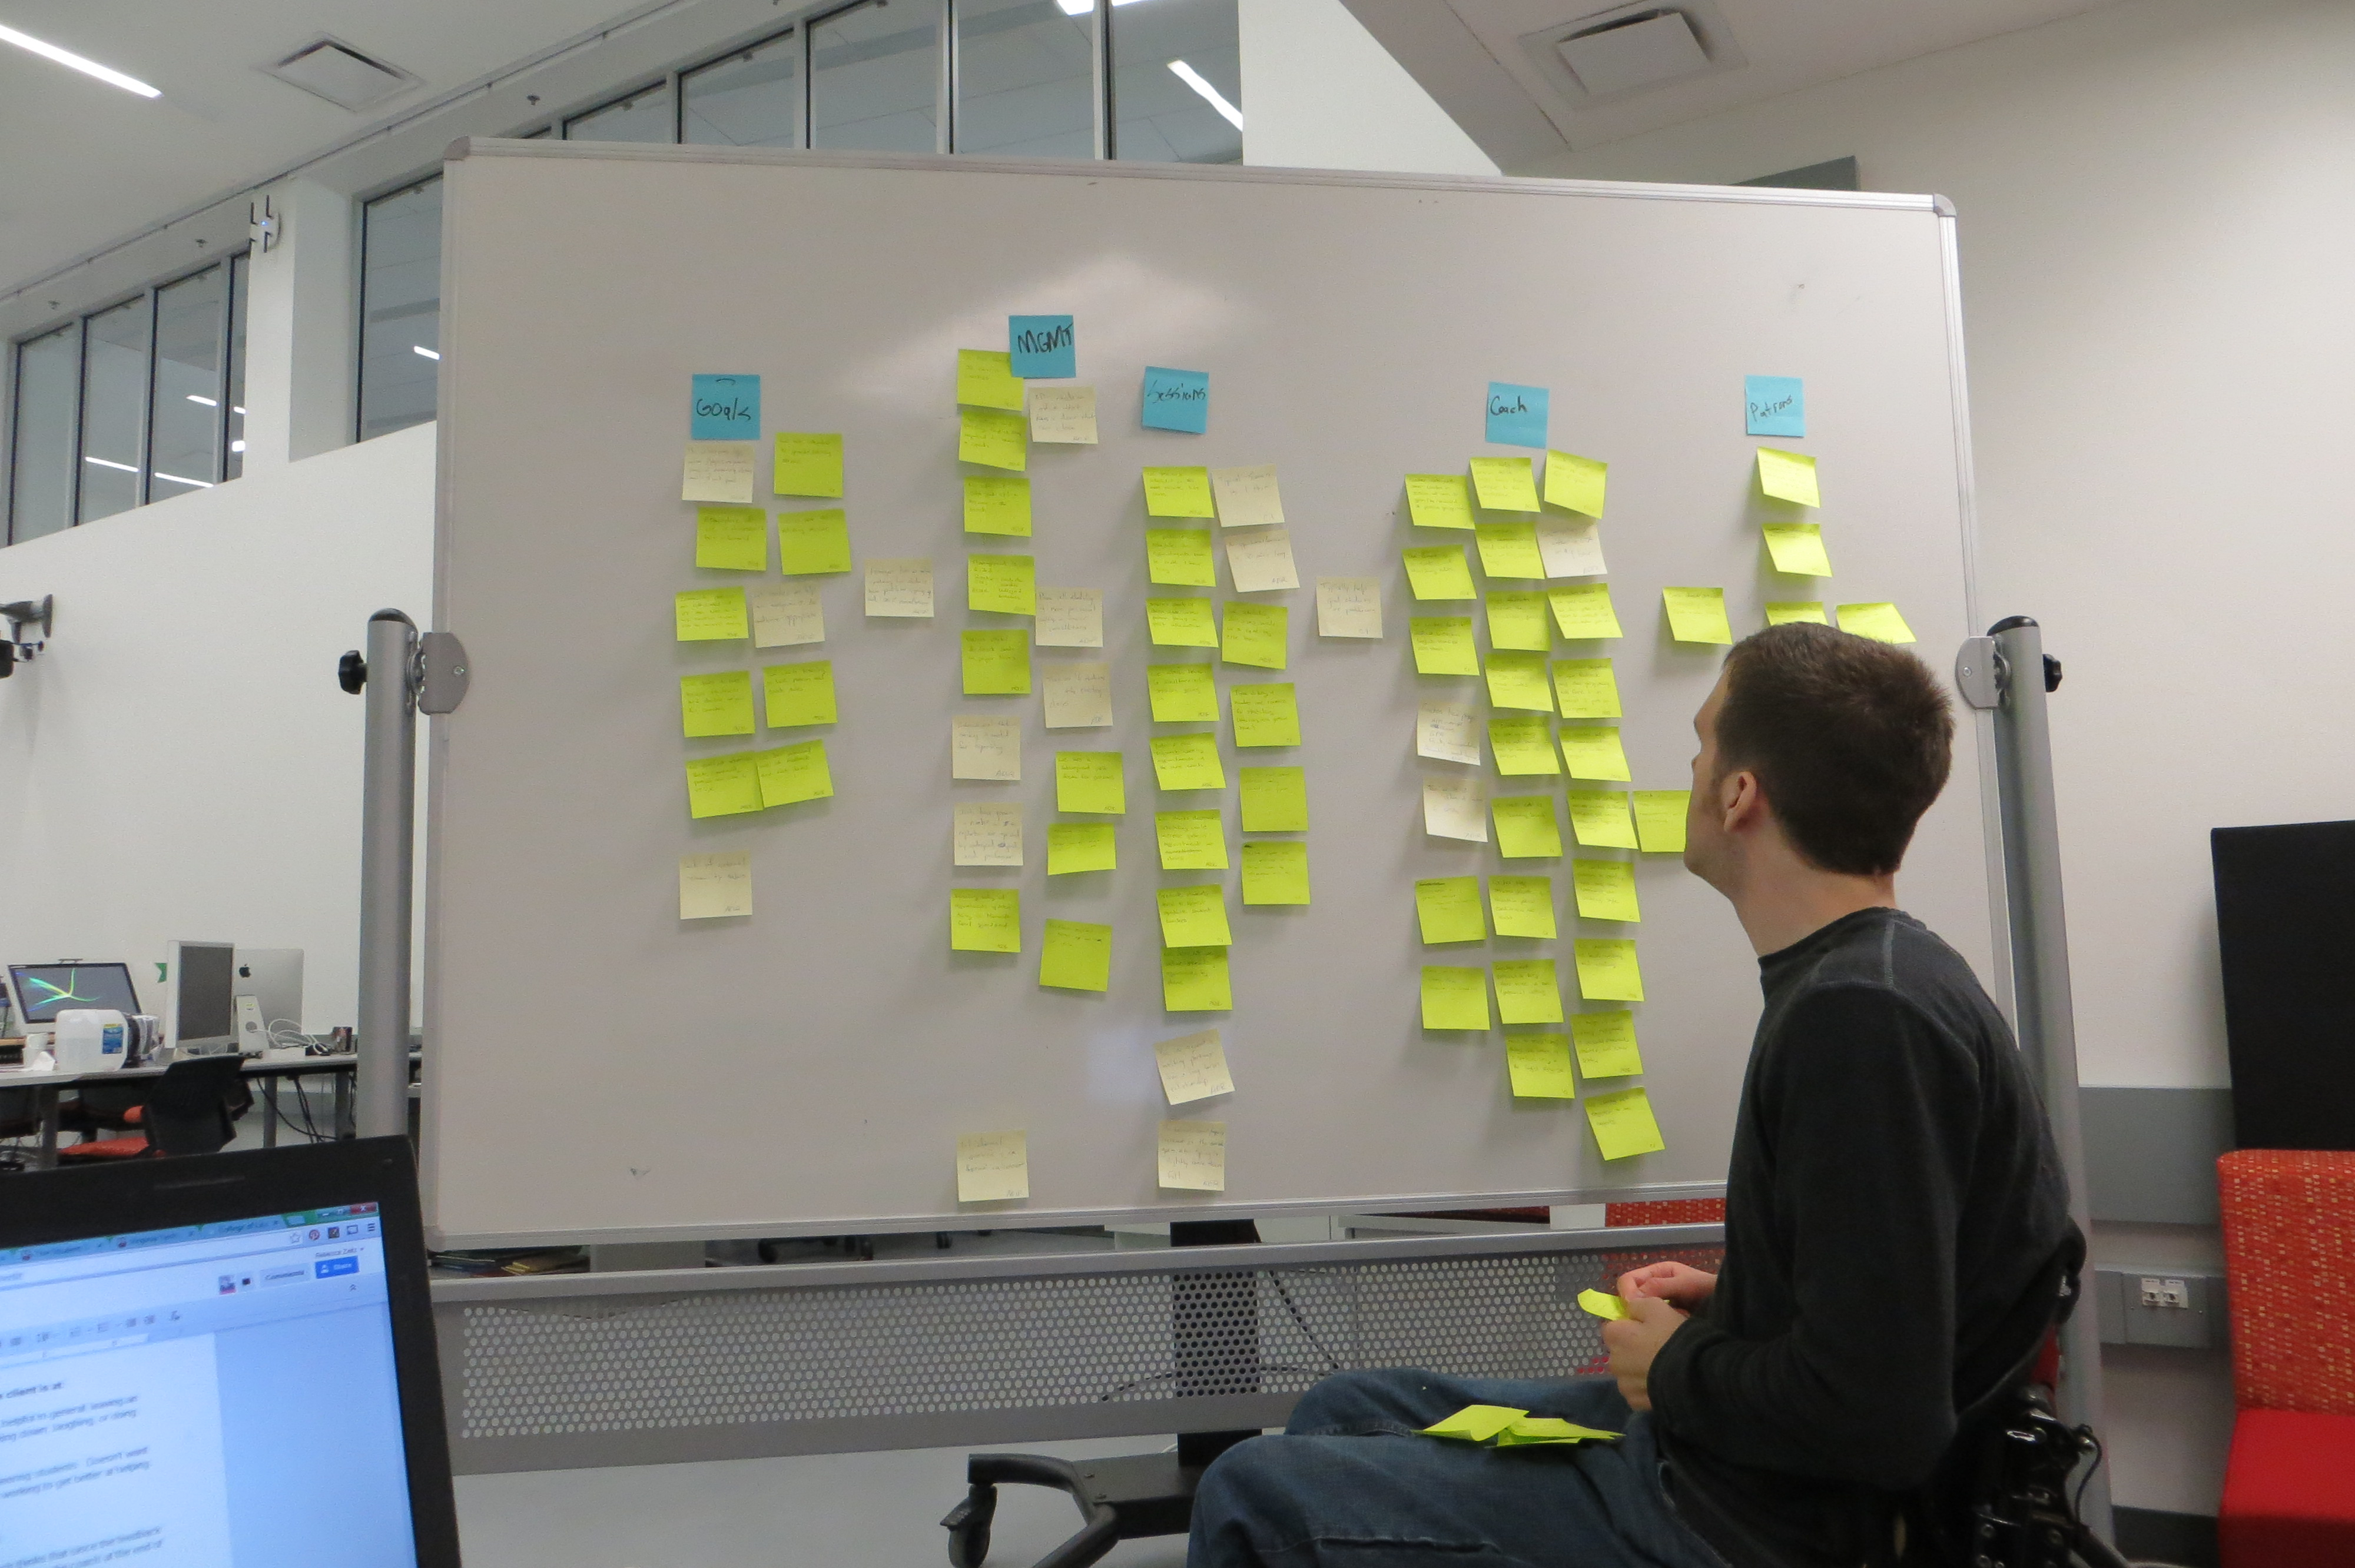
\includegraphics[width=0.95\linewidth]{TeamAtWork1}
      \caption{T.C. at the WAAD}
      \label{fig:team_photo_1}
    \end{subfigure}%
    \begin{subfigure}{.5\linewidth}
      \centering
      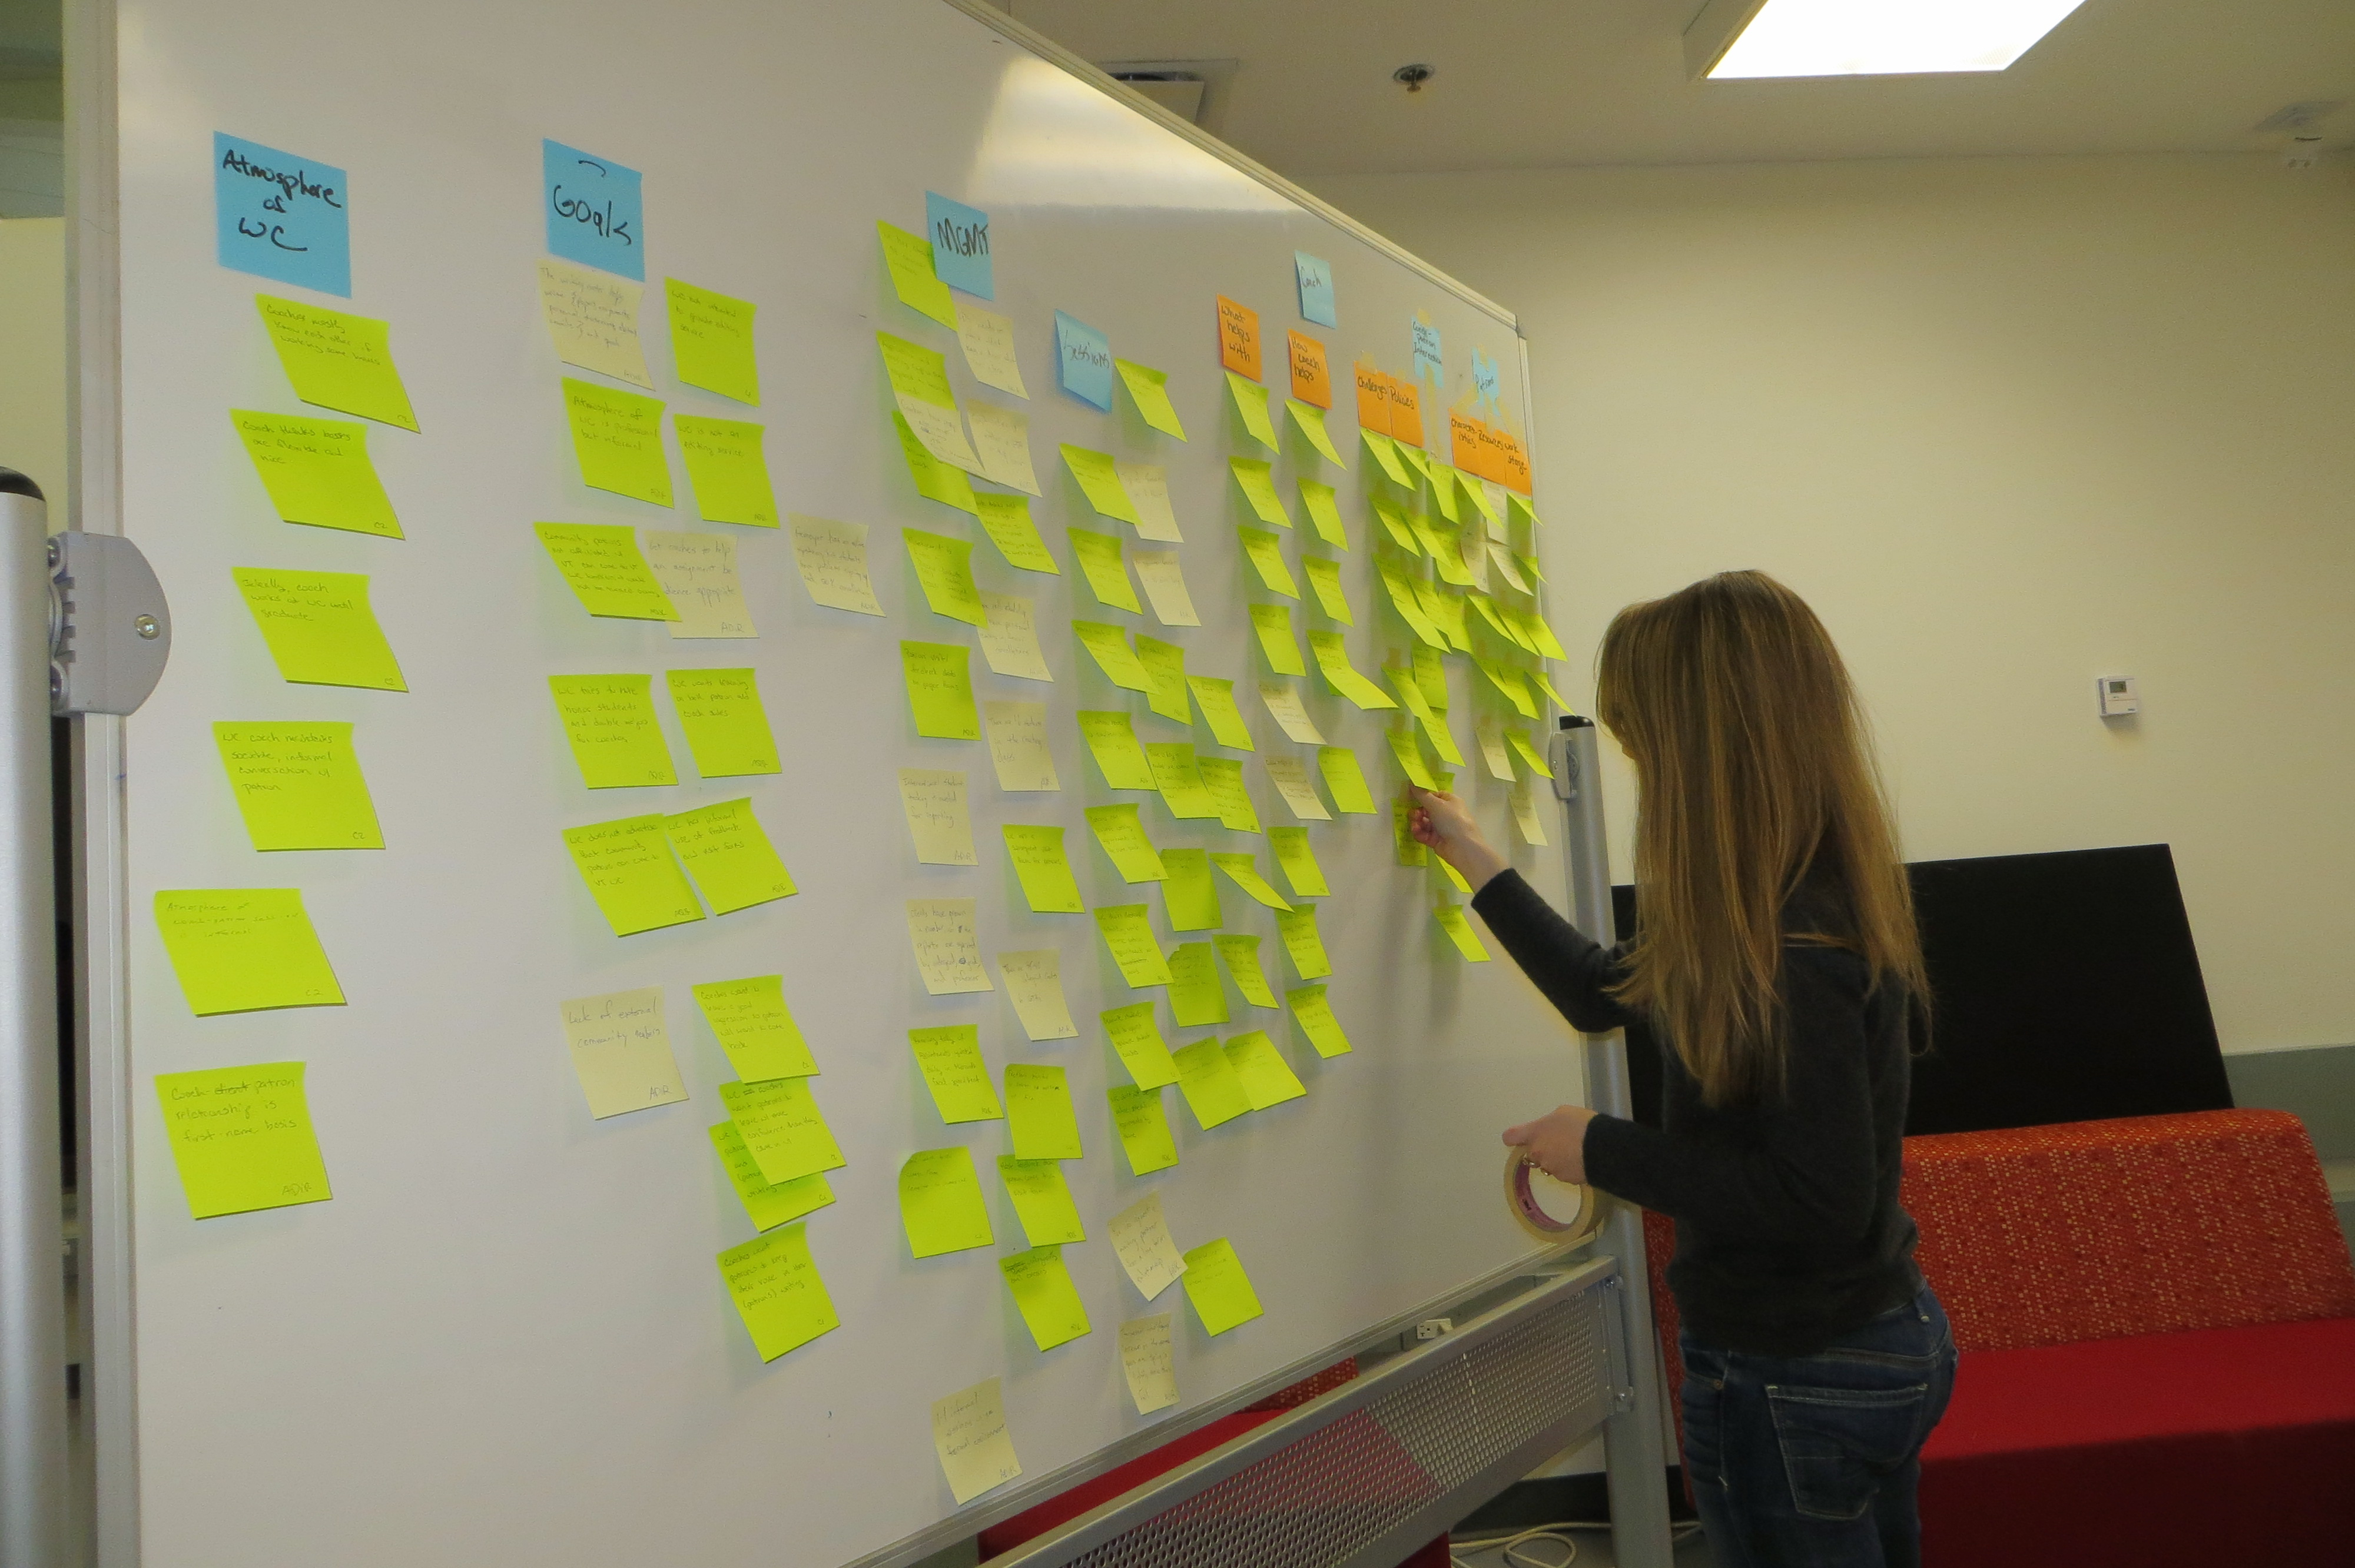
\includegraphics[width=0.95\linewidth]{TeamAtWork3}
      \caption{Rebecca at the WAAD}
      \label{fig:team_photo_3}
    \end{subfigure}\\[1ex]
    \begin{subfigure}{\linewidth}
      \centering
      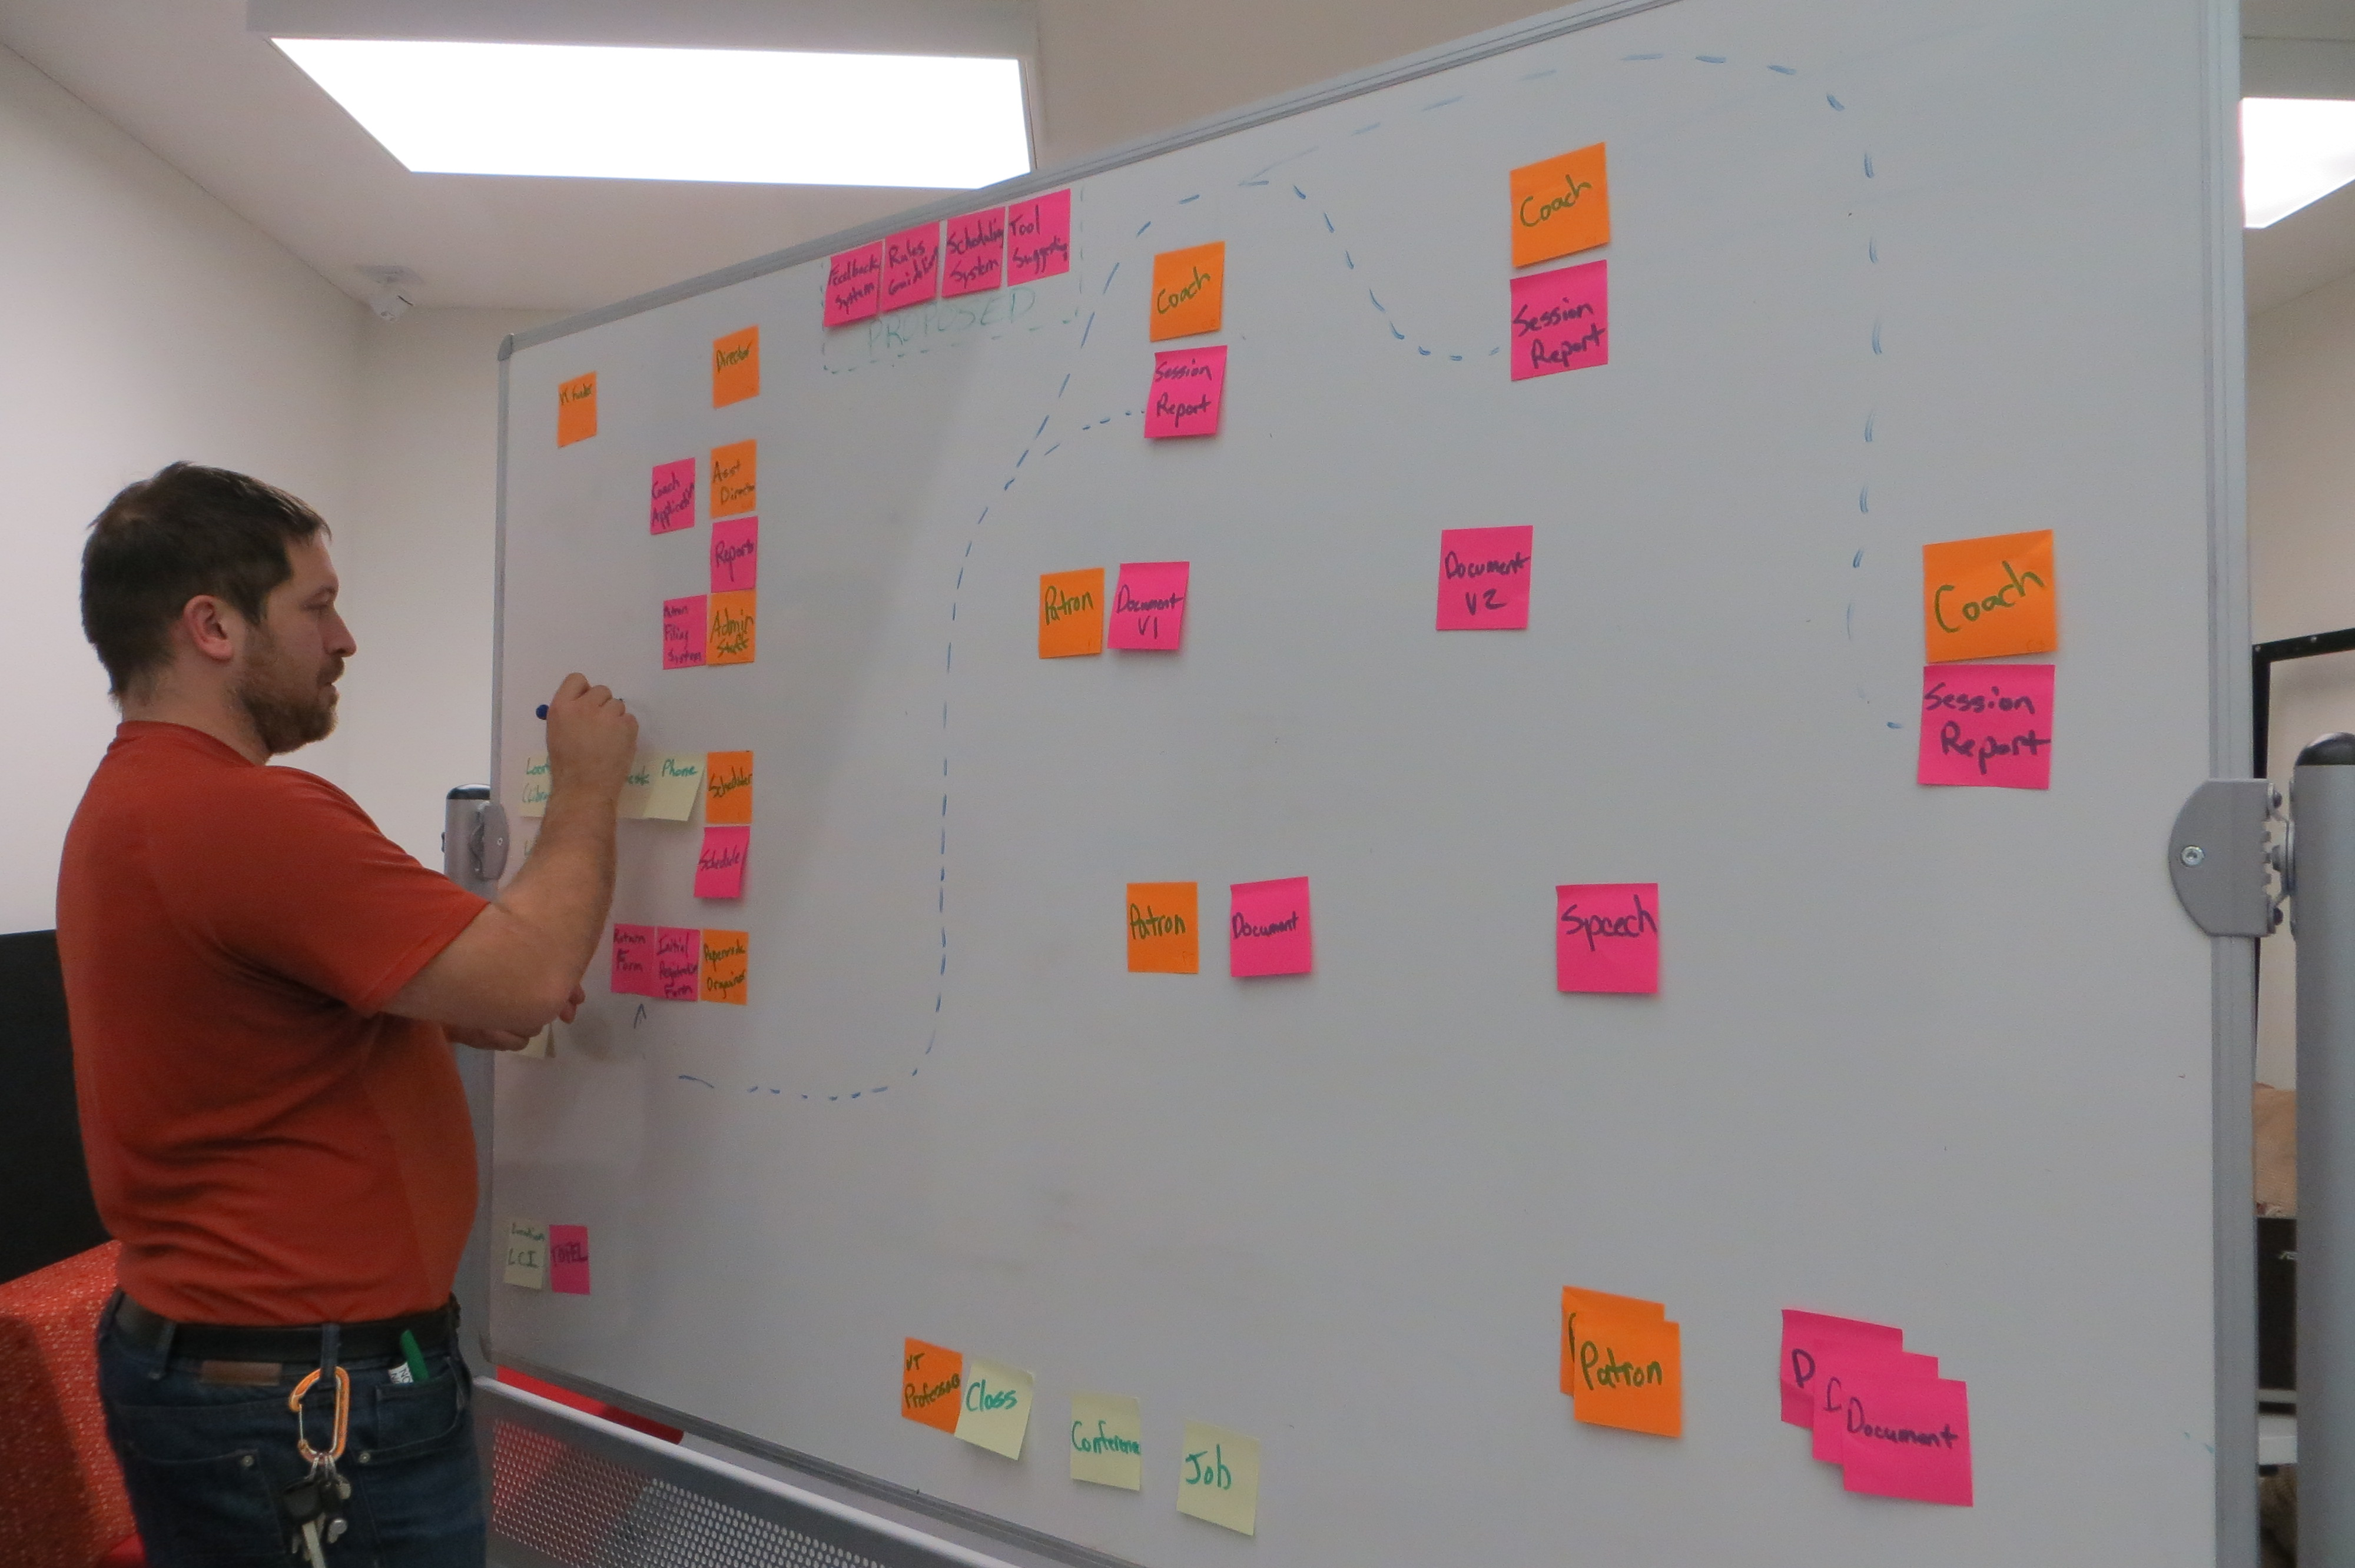
\includegraphics[width=0.55\linewidth]{TeamAtWork4}
      \caption{Chris at the flow model diagram}
      \label{fig:team_photo_4}
    \end{subfigure}
    \caption{The team in action}
    \label{fig:test}
  \end{figure}

\section{WAAD Photos} %15
% Include a few photos of your WAAD. 
  \begin{figure}[H]
    \begin{subfigure}{.5\linewidth}
      \centering
      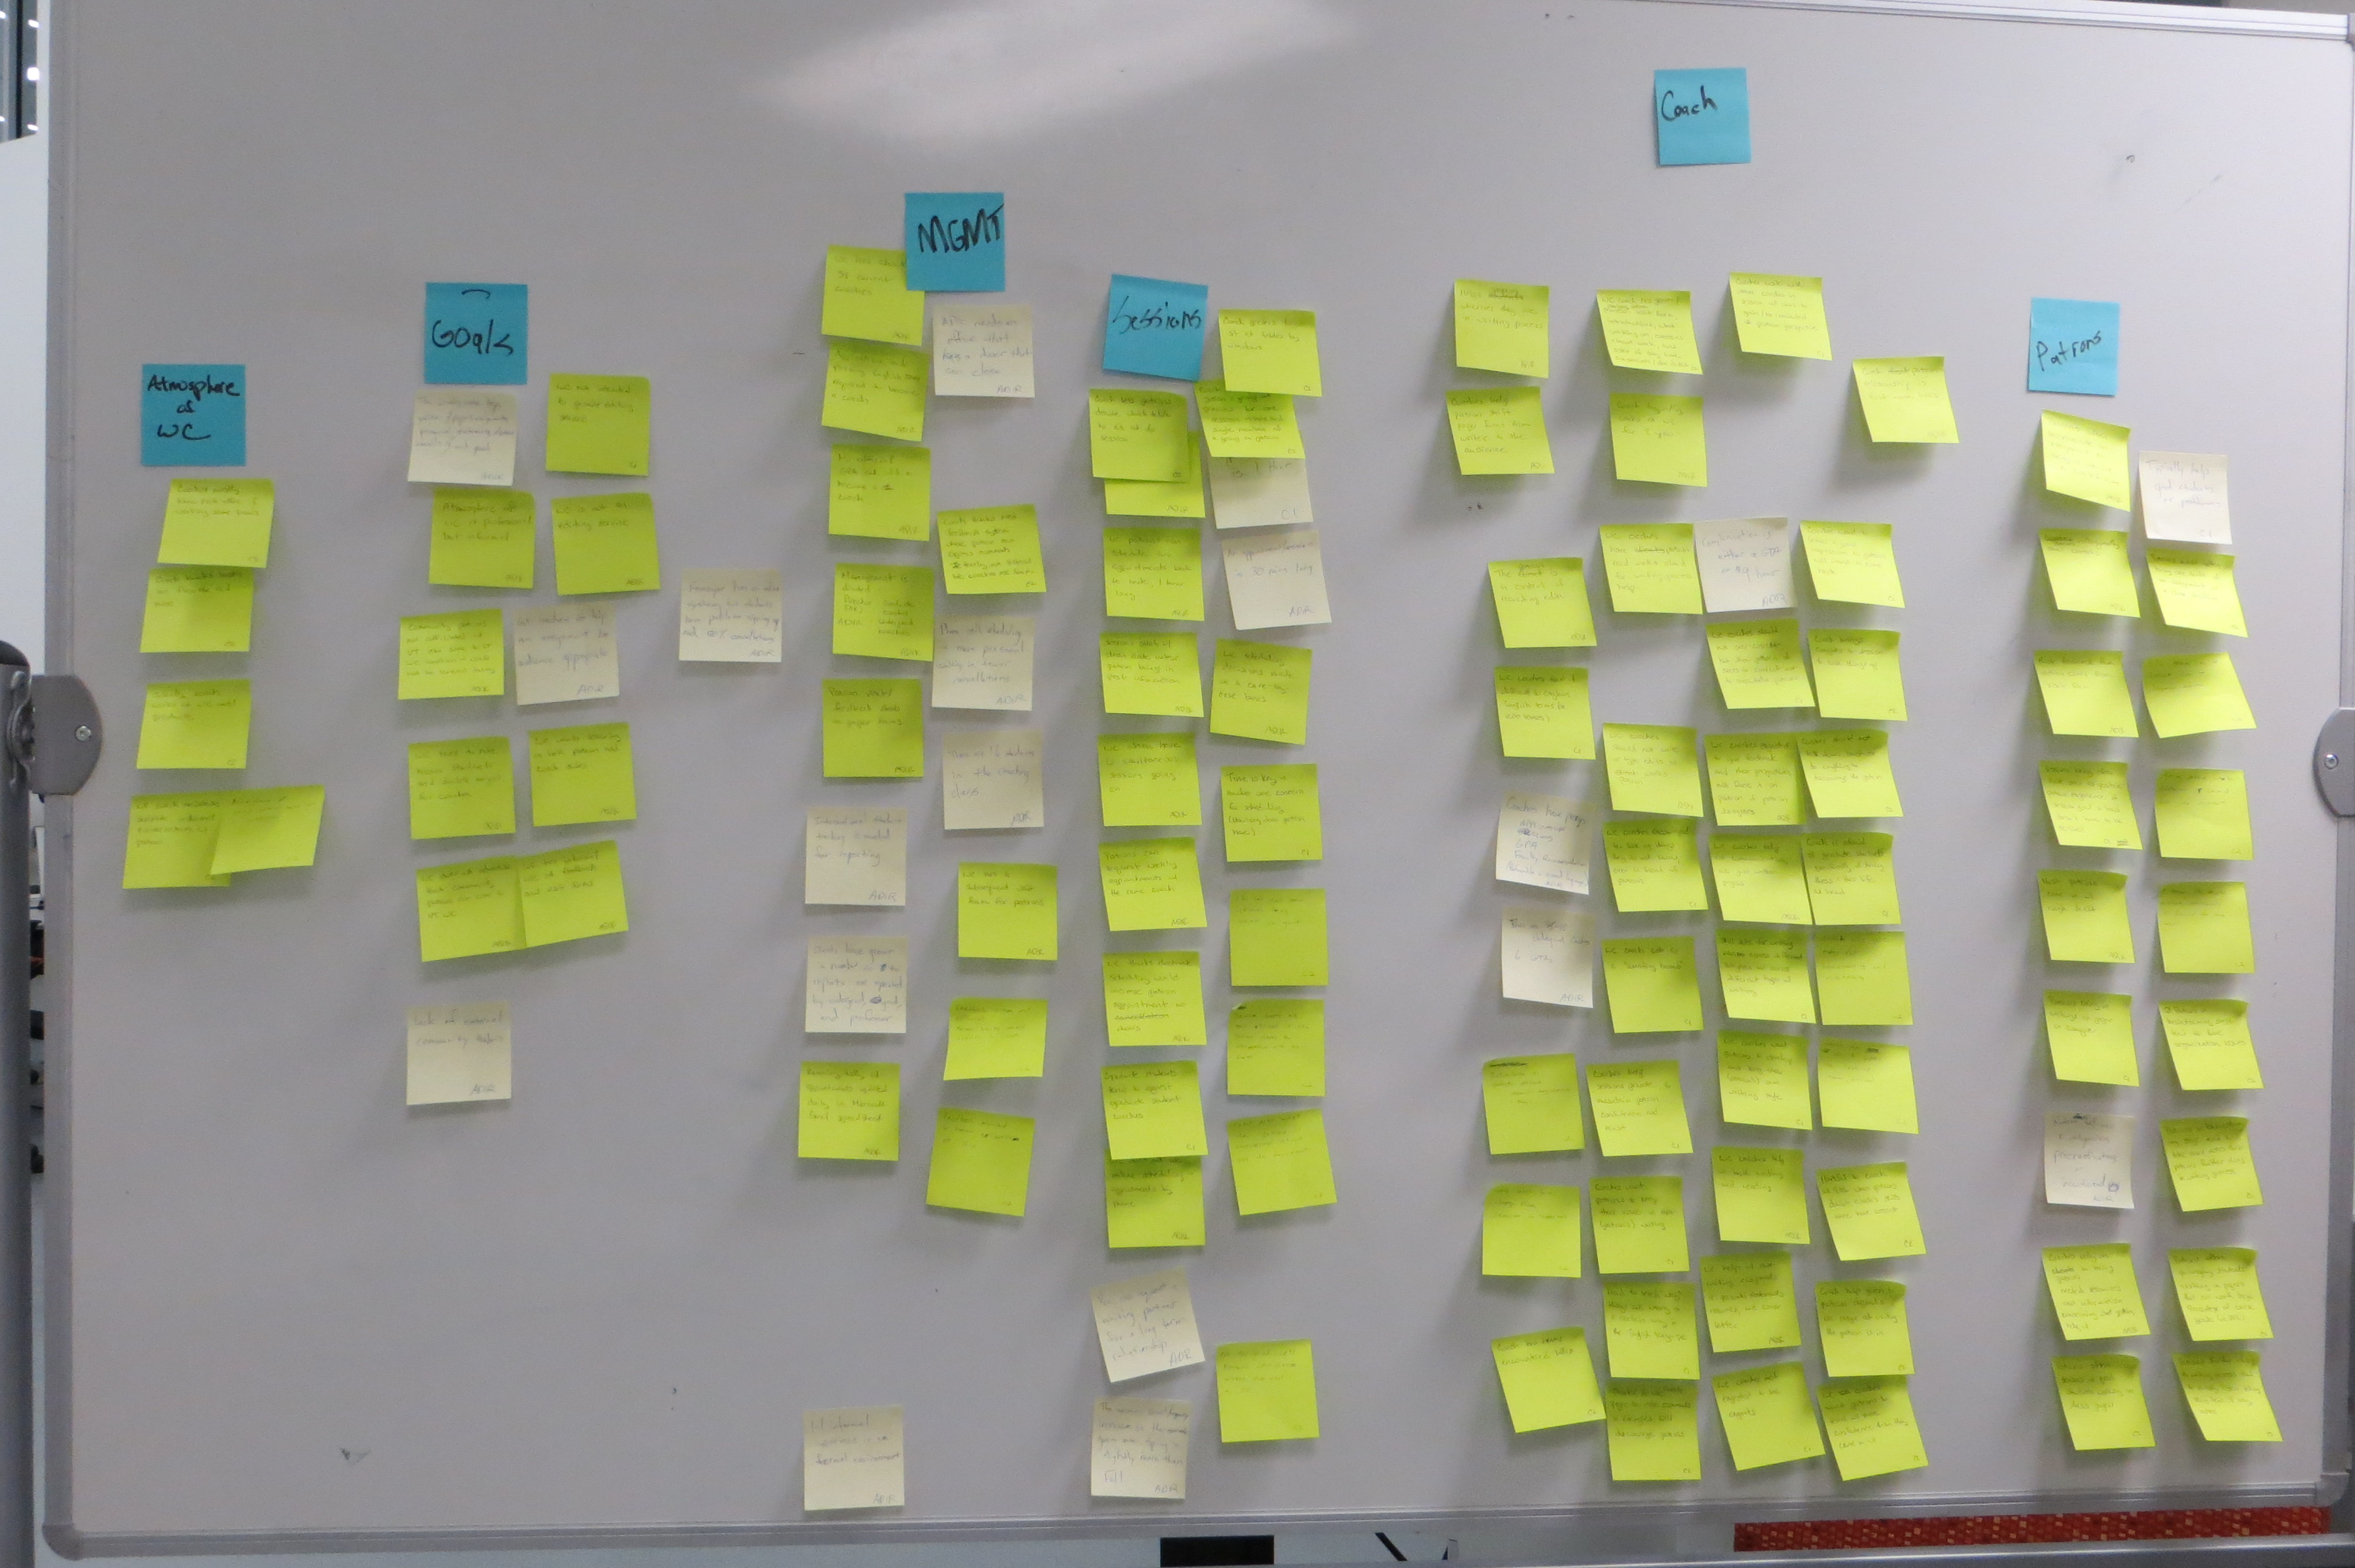
\includegraphics[width=0.95\linewidth]{WAAD_version1}
      \caption{Phase 1}
      \label{fig:WAAD_version1}
    \end{subfigure}%
    \begin{subfigure}{.5\linewidth}
      \centering
      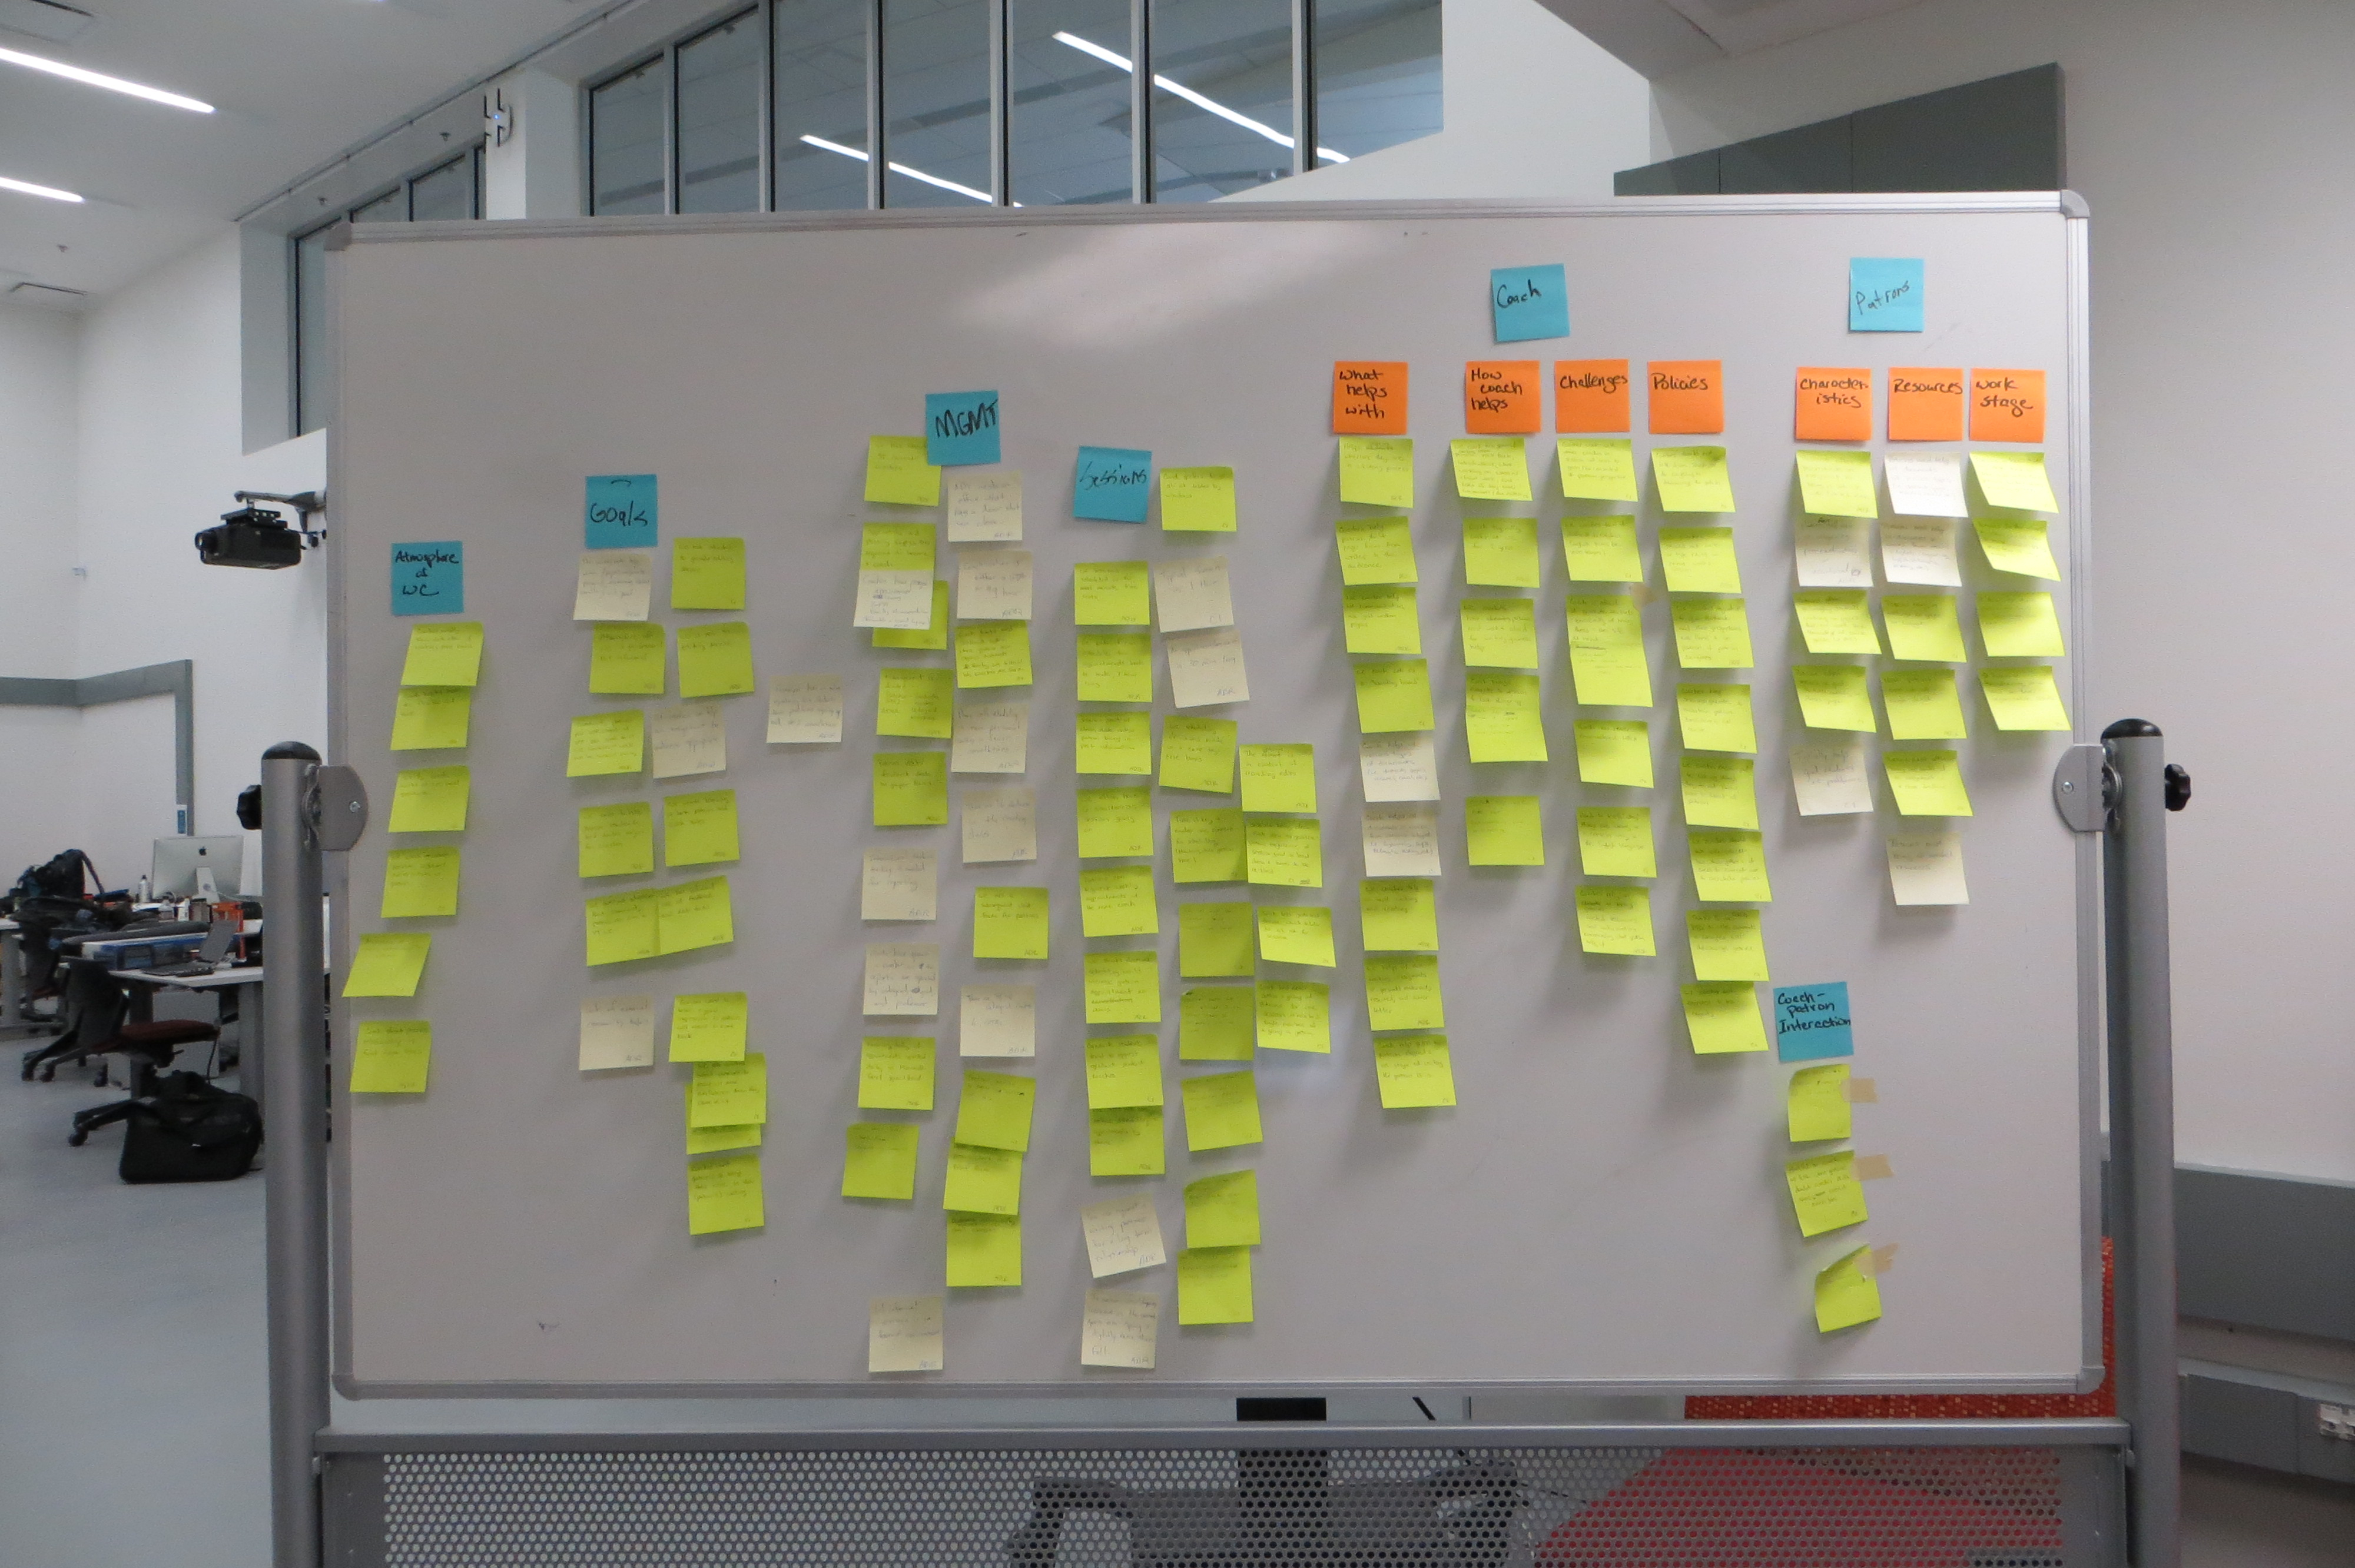
\includegraphics[width=0.95\linewidth]{WAAD_version2}
      \caption{Phase 2}
      \label{fig:WAAD_version2}
    \end{subfigure}\\[1ex]
    \begin{subfigure}{.5\linewidth}
      \centering
      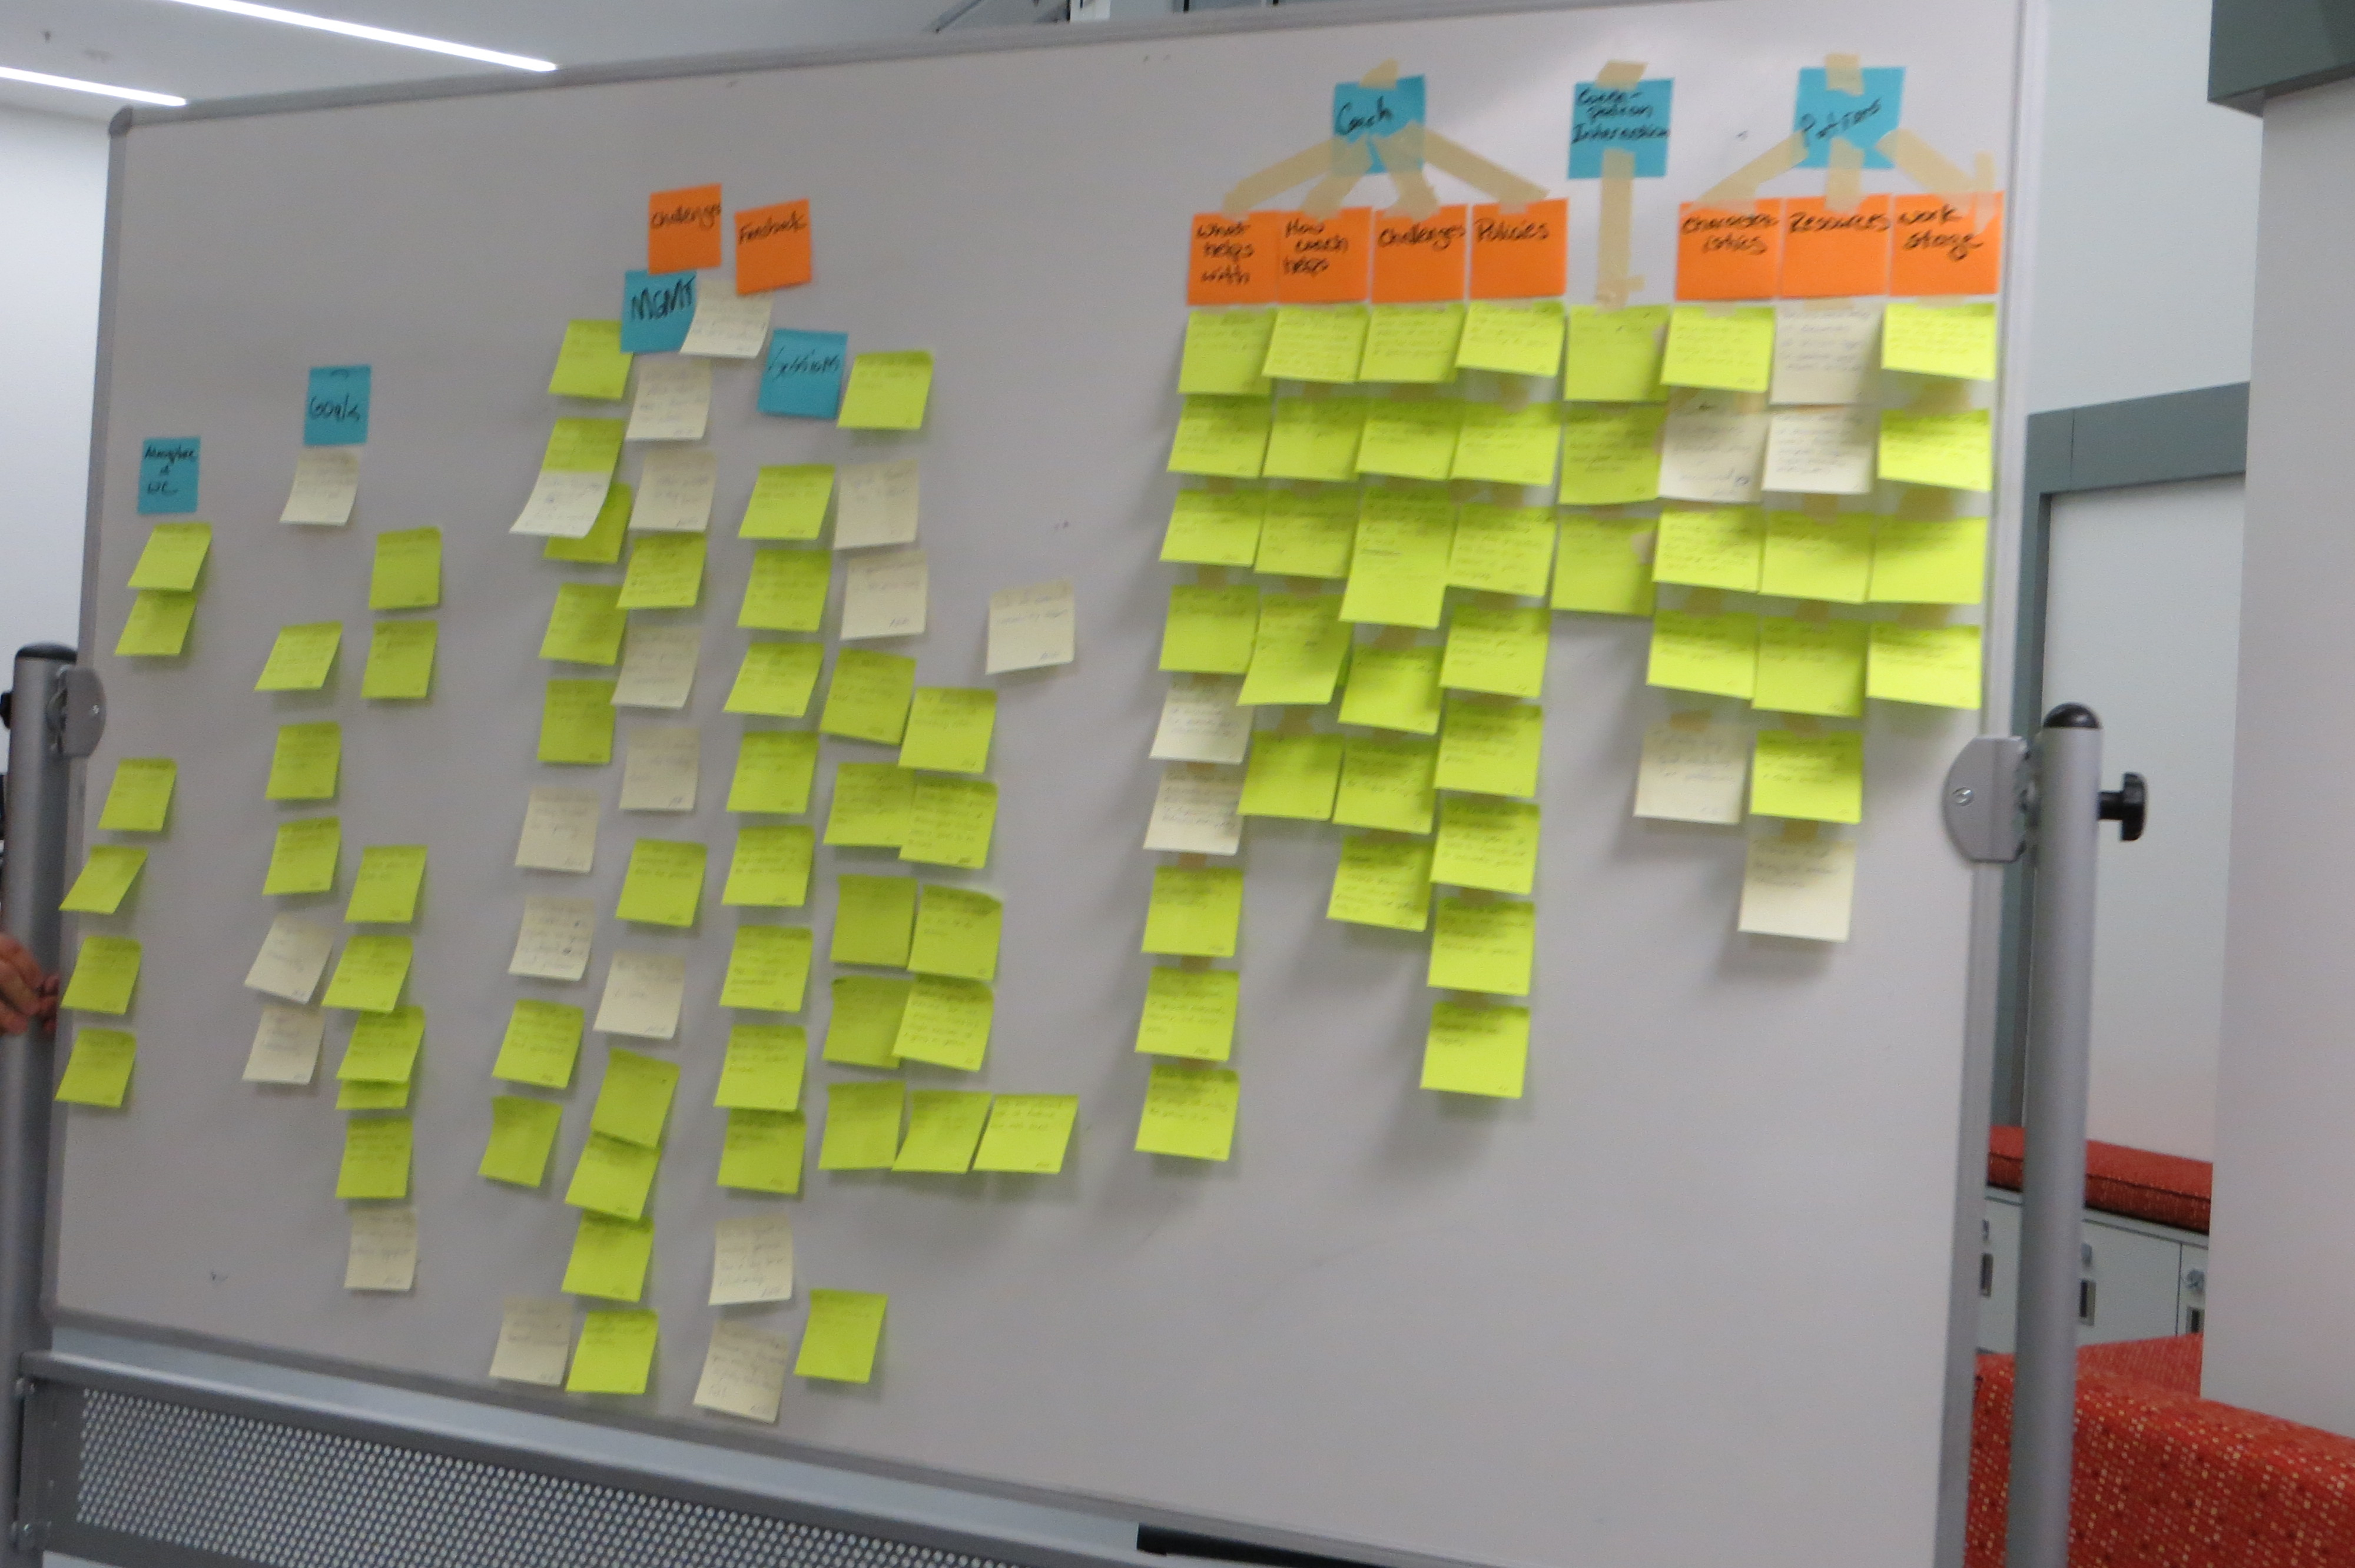
\includegraphics[width=0.95\linewidth]{WAAD_version3}
      \caption{Phase 3}
      \label{fig:WAAD_version3}
    \end{subfigure}%
    \begin{subfigure}{.5\linewidth}
      \centering
      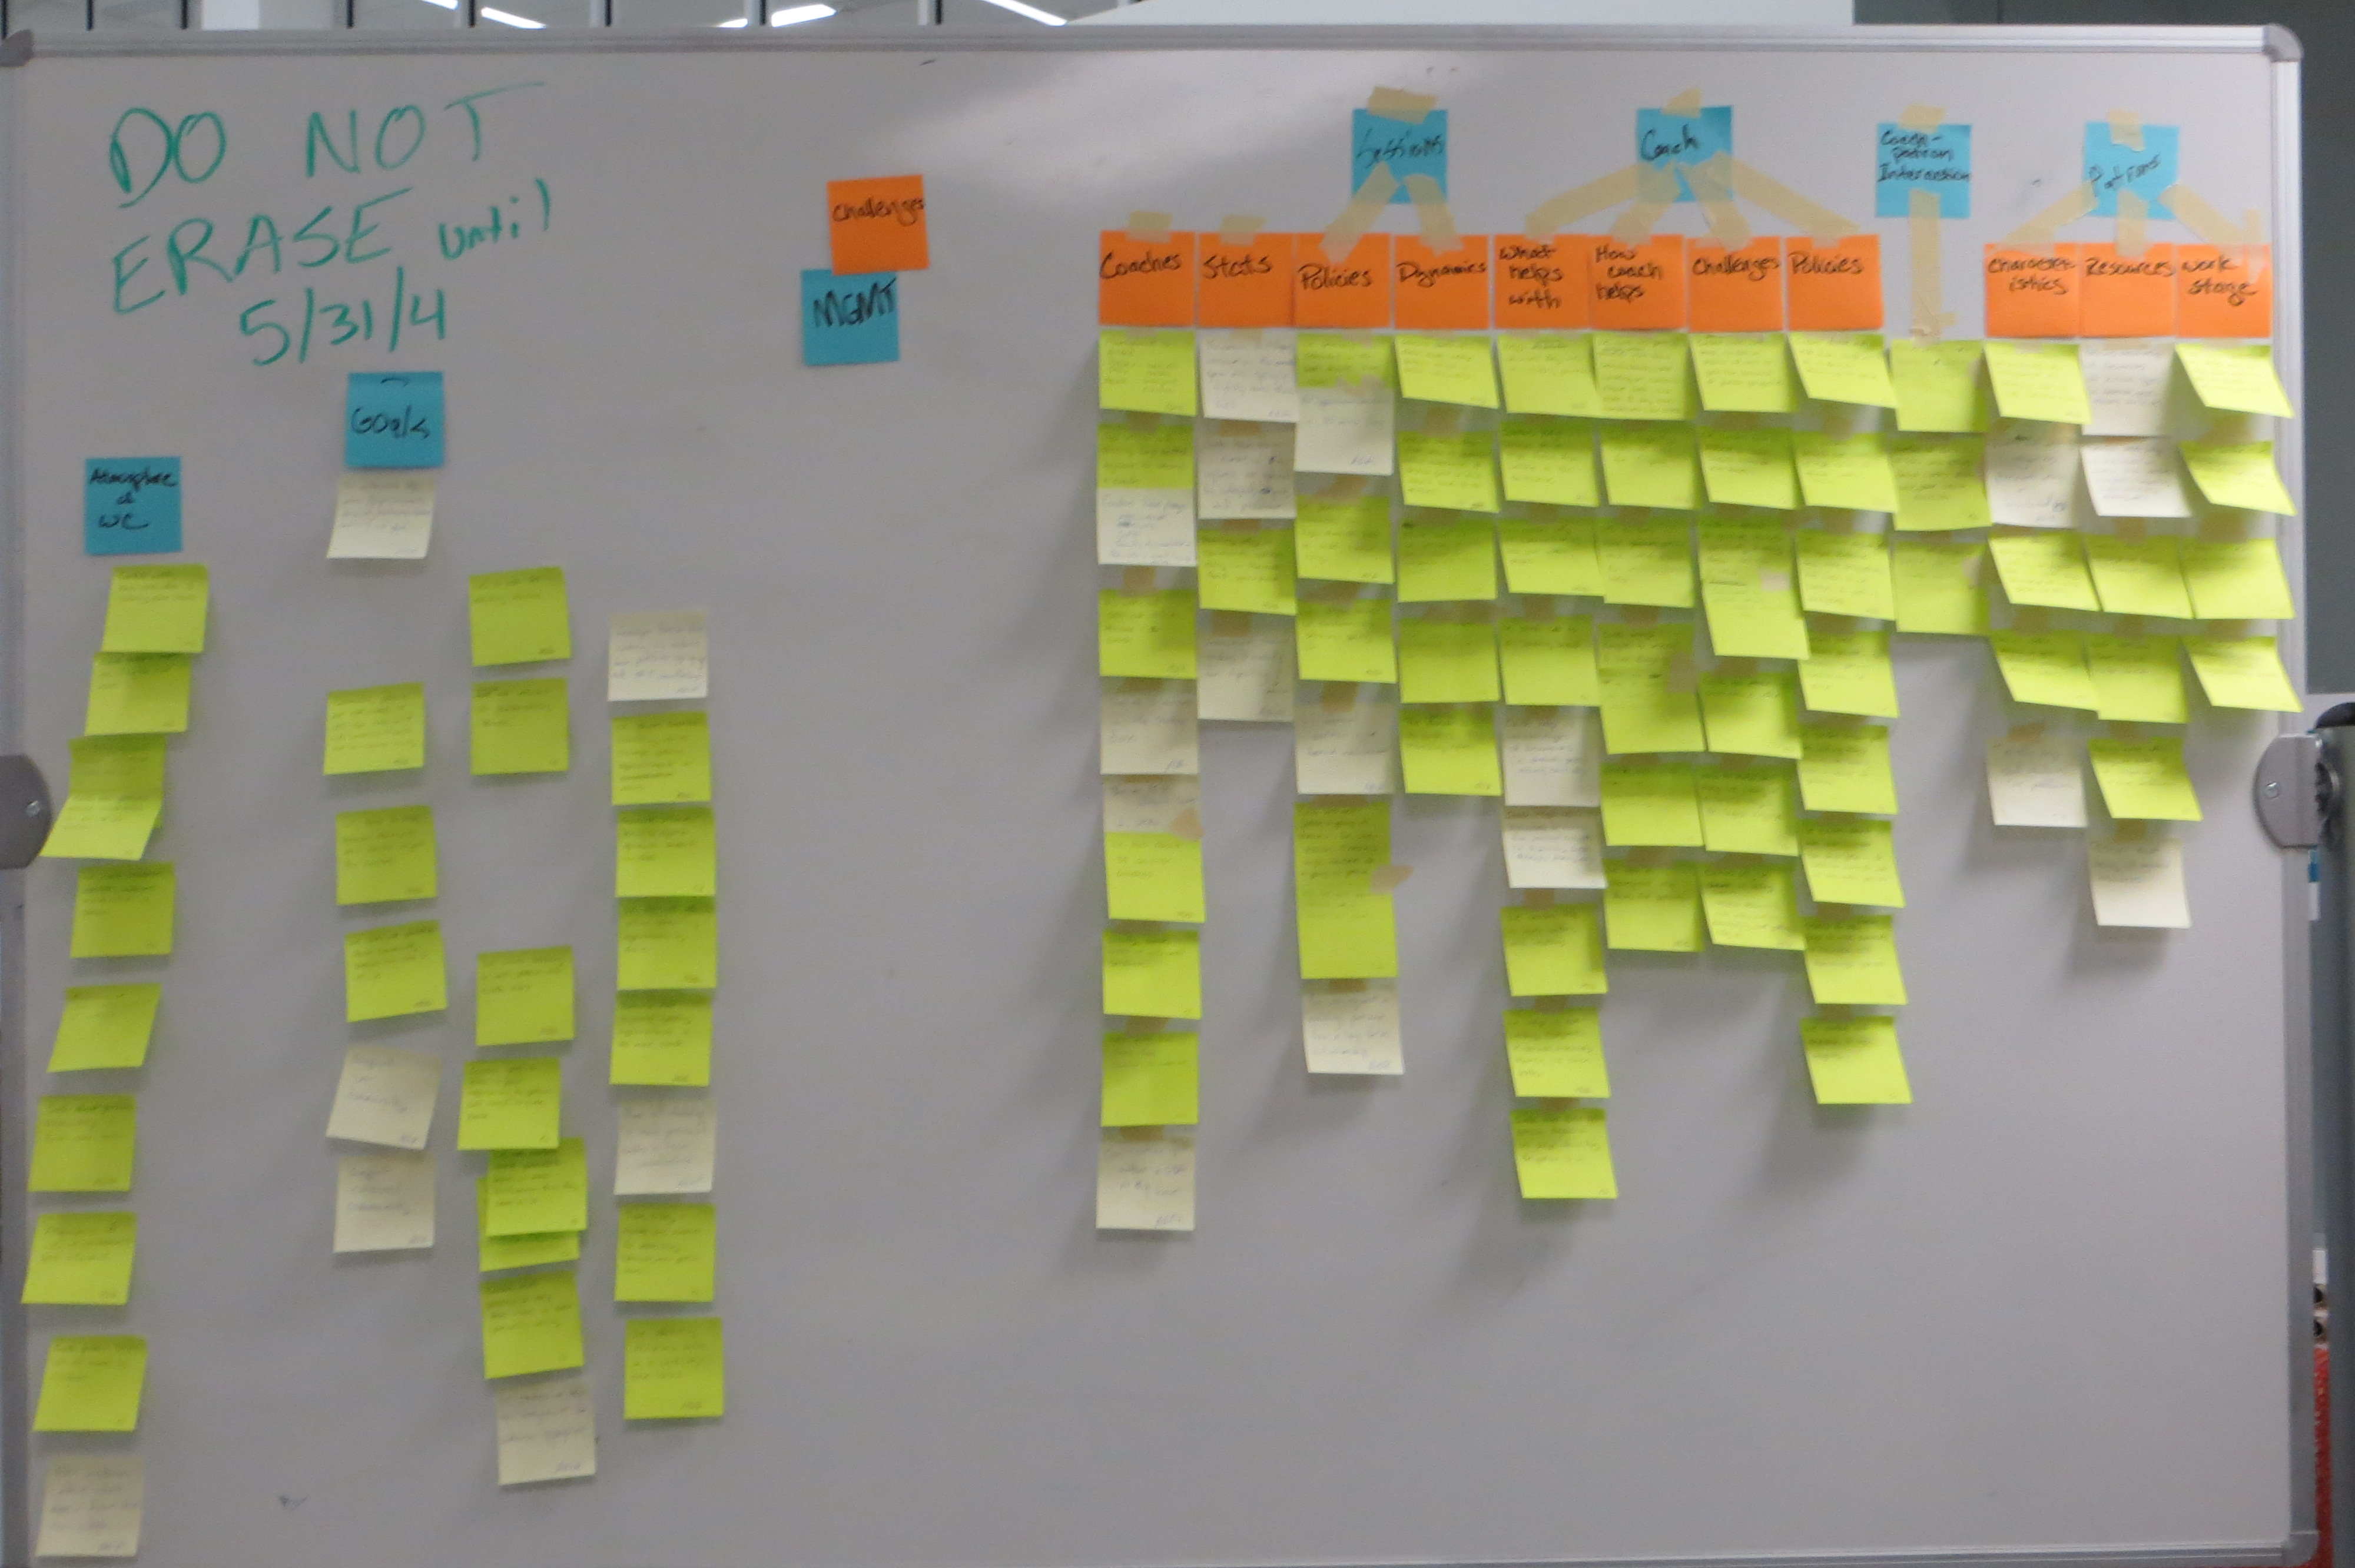
\includegraphics[width=0.95\linewidth]{WAAD_version4}
      \caption{Phase 4}
      \label{fig:WAAD_version4}
    \end{subfigure}\\[1ex]
    \begin{subfigure}{\linewidth}
      \centering
      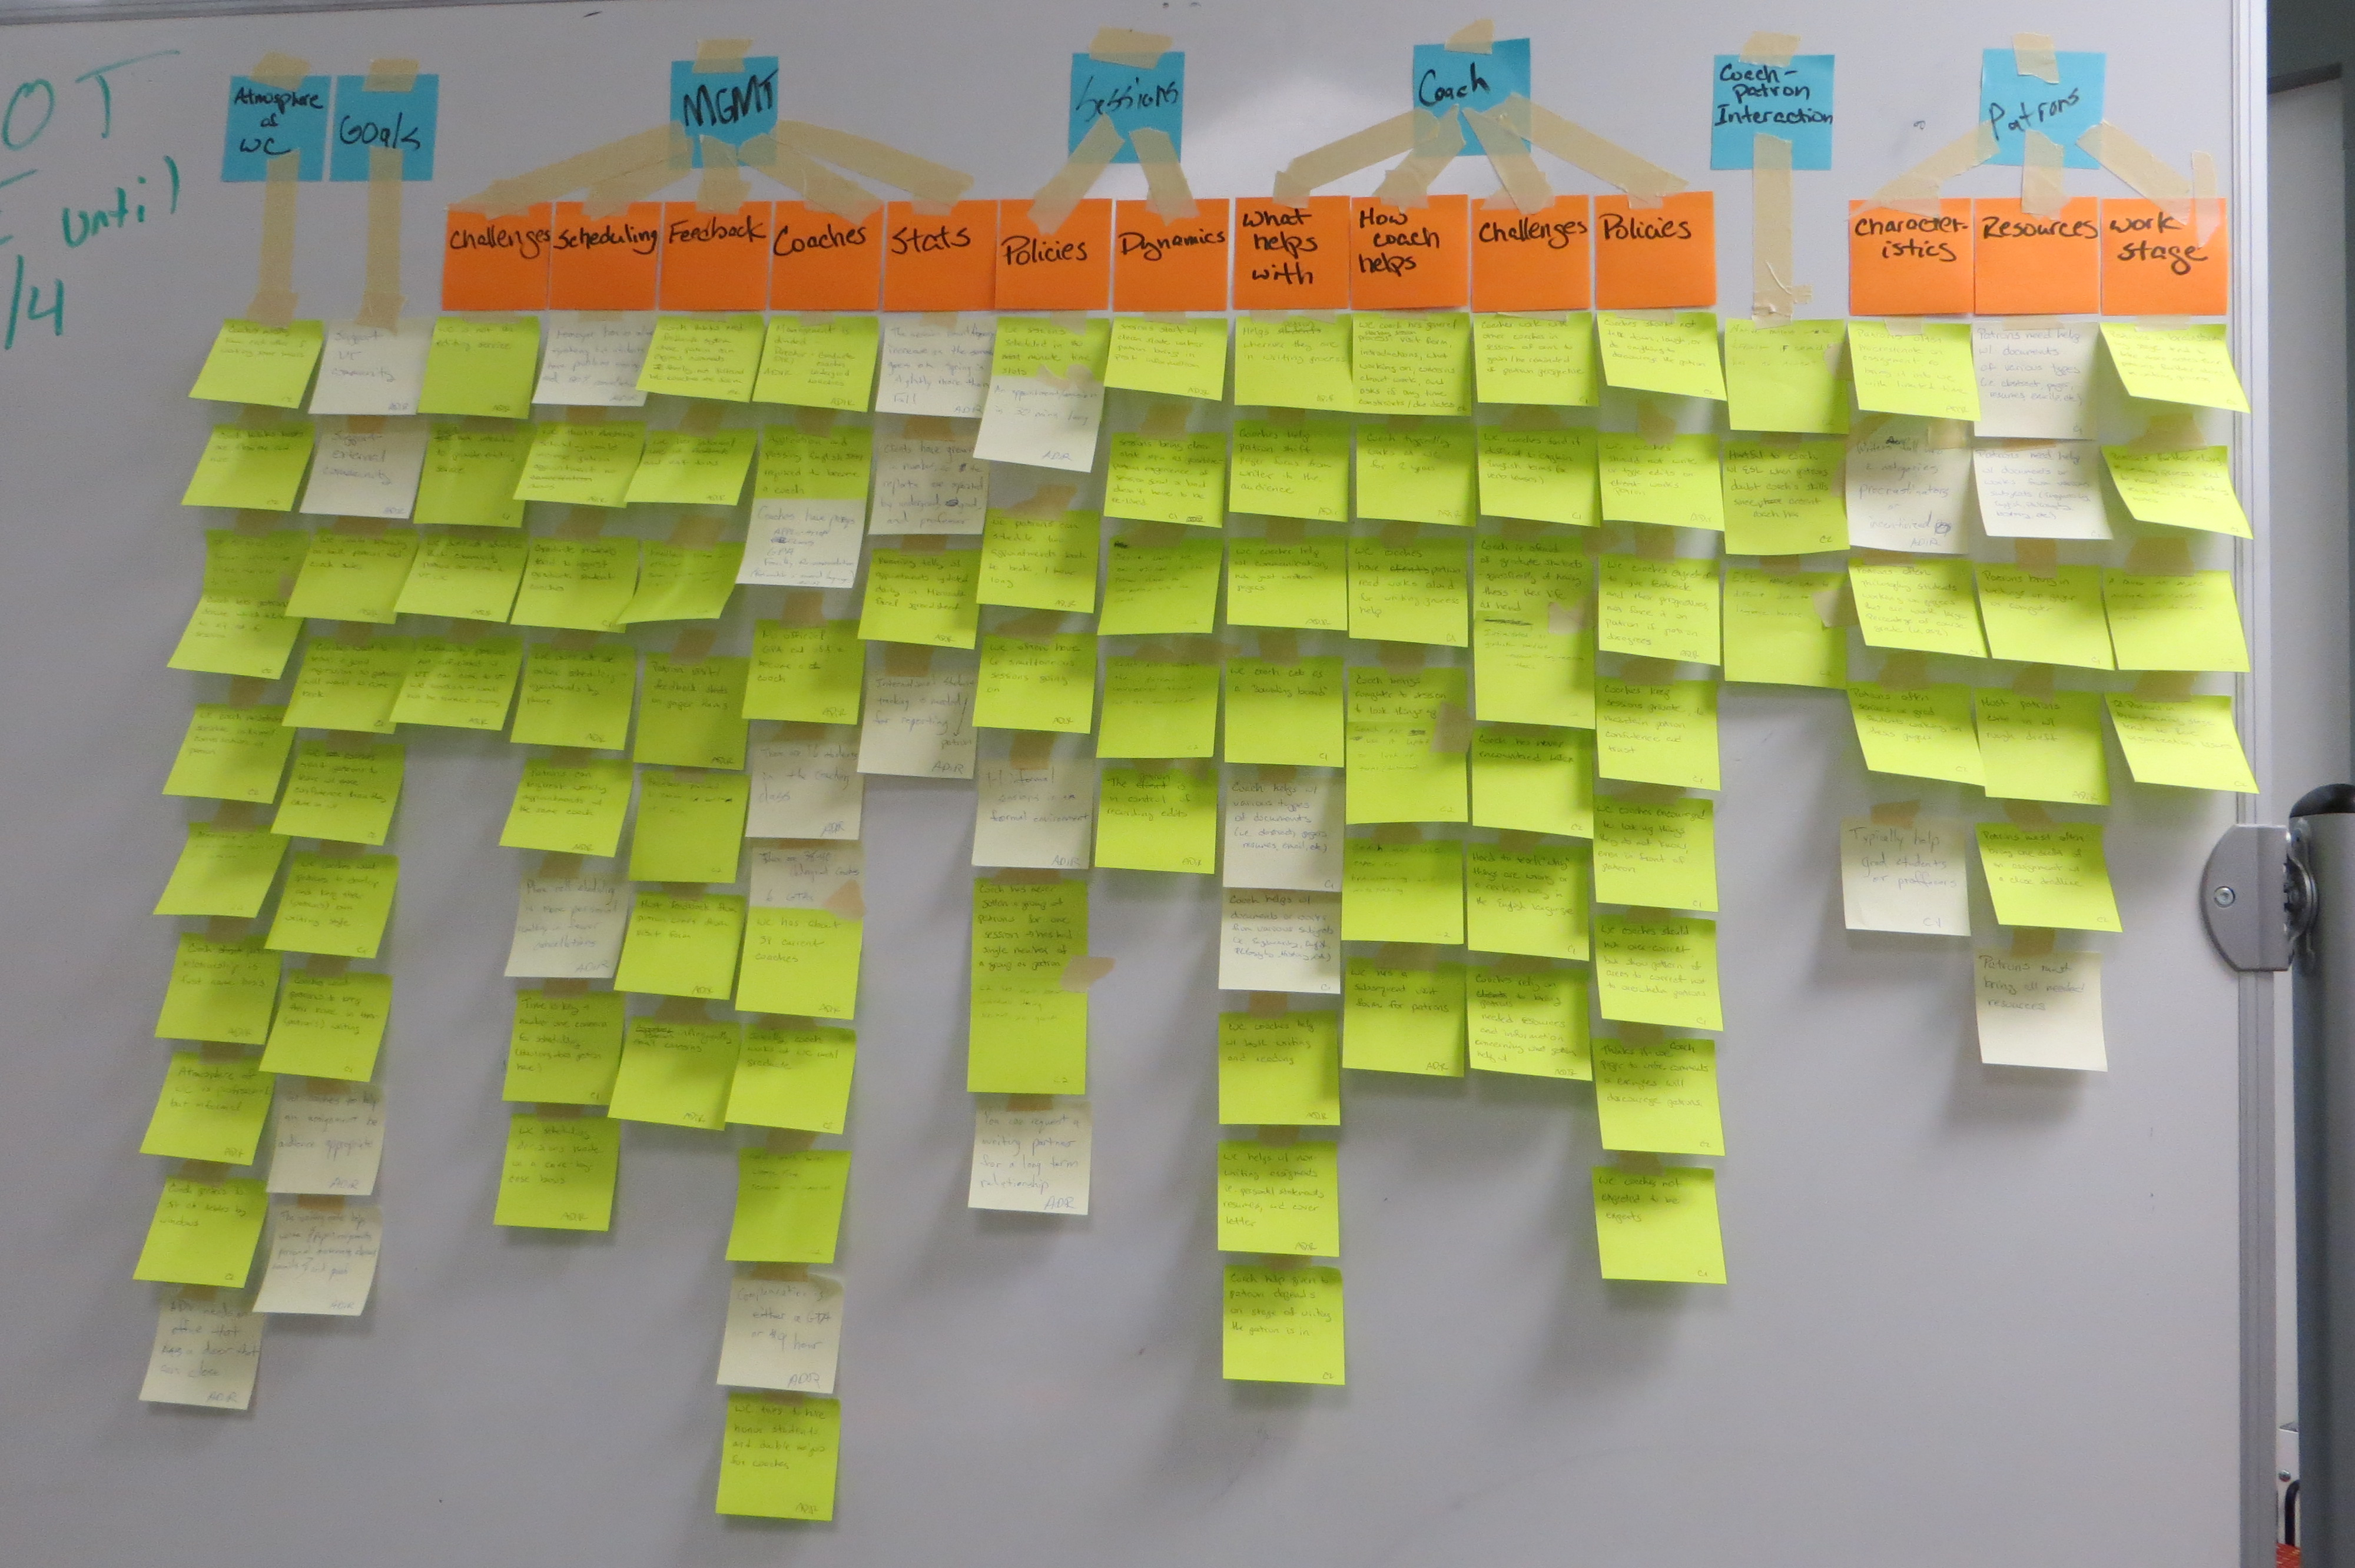
\includegraphics[width=0.55\linewidth]{WAAD_version5}
      \caption{Phase 5}
      \label{fig:WAAD_version5}
    \end{subfigure}
    \caption{Evolution of the WAAD}
    \label{fig:WAAD}
  \end{figure}

\section{Work Roles} %16
% List and describe each of the major work roles, sub-roles, and machine roles. 
  Work roles are noted as orange squares in the work flow figure of \ref{fig:Workflow_final}.
  \begin{description} % Numbered list example
  \item[Director]
  Diana George
  \item[Assistant Director]
  Jennifer Lawrence (7 years in this position)\\
  The Assistant Director is in charge of hiring all coaches, scheduling coach work allotments, reports, a
  \item[Administrative Staff]
  Sandra Ross \\
  This role is in charge of making the consolidated reports and trends that are received from the Scheduler, and providing administrative assistance to the Director and Assistant Director. 
  \item[Graduate Assistant to the Director]
  Katharine Torrey \\
  This is a coach who in addition to normal coach role duties, also helps with some of the tasks that are oriented towards the coaches, speaking as a representative for the coaches and a supporting voice for the Assistant Director.
  \item[Coach] \hfill \\
  These are undergraduate and graduate students who have a strong skill set in the English language.
  They are required to have an application, strong GPA, a letter of recommendation from a VT faculty member , and have passed the English 3744 class.
  Ideally a second language, double major, and/or honor student.
  \item[Patron] \hfill \\
  Any local resident of the New River Valley, with or without VT affiliation, who wants help improving their communication skills (writing, grammar, speech, and culture).
  \item[VT Professor] \hfill \\
  A professor or lecturer at Virginia Tech.
  \item[Scheduler] \hfill \\
  A coach at the WC that is currently not seeing a patron, who makes appointments in the schedule book.
  \item[Paperwork Organizer] \hfill \\
  A coach at the WC that is currently not seeing a patron, who arranges the session paperwork to hand to the Admin person.
  \item[Funding] \hfill \\
  People or entities, predominately but not always affiliated with VT, that provide monetary funds to the WC for operational costs.
  \end{description} 

\section{Flow Model Diagram} %17
% Show your initial flow model diagram. This should be described from a broad view, not just the flow addressed by your system.
  \begin{figure}[H]
    \begin{subfigure}{.5\linewidth}
      \centering
      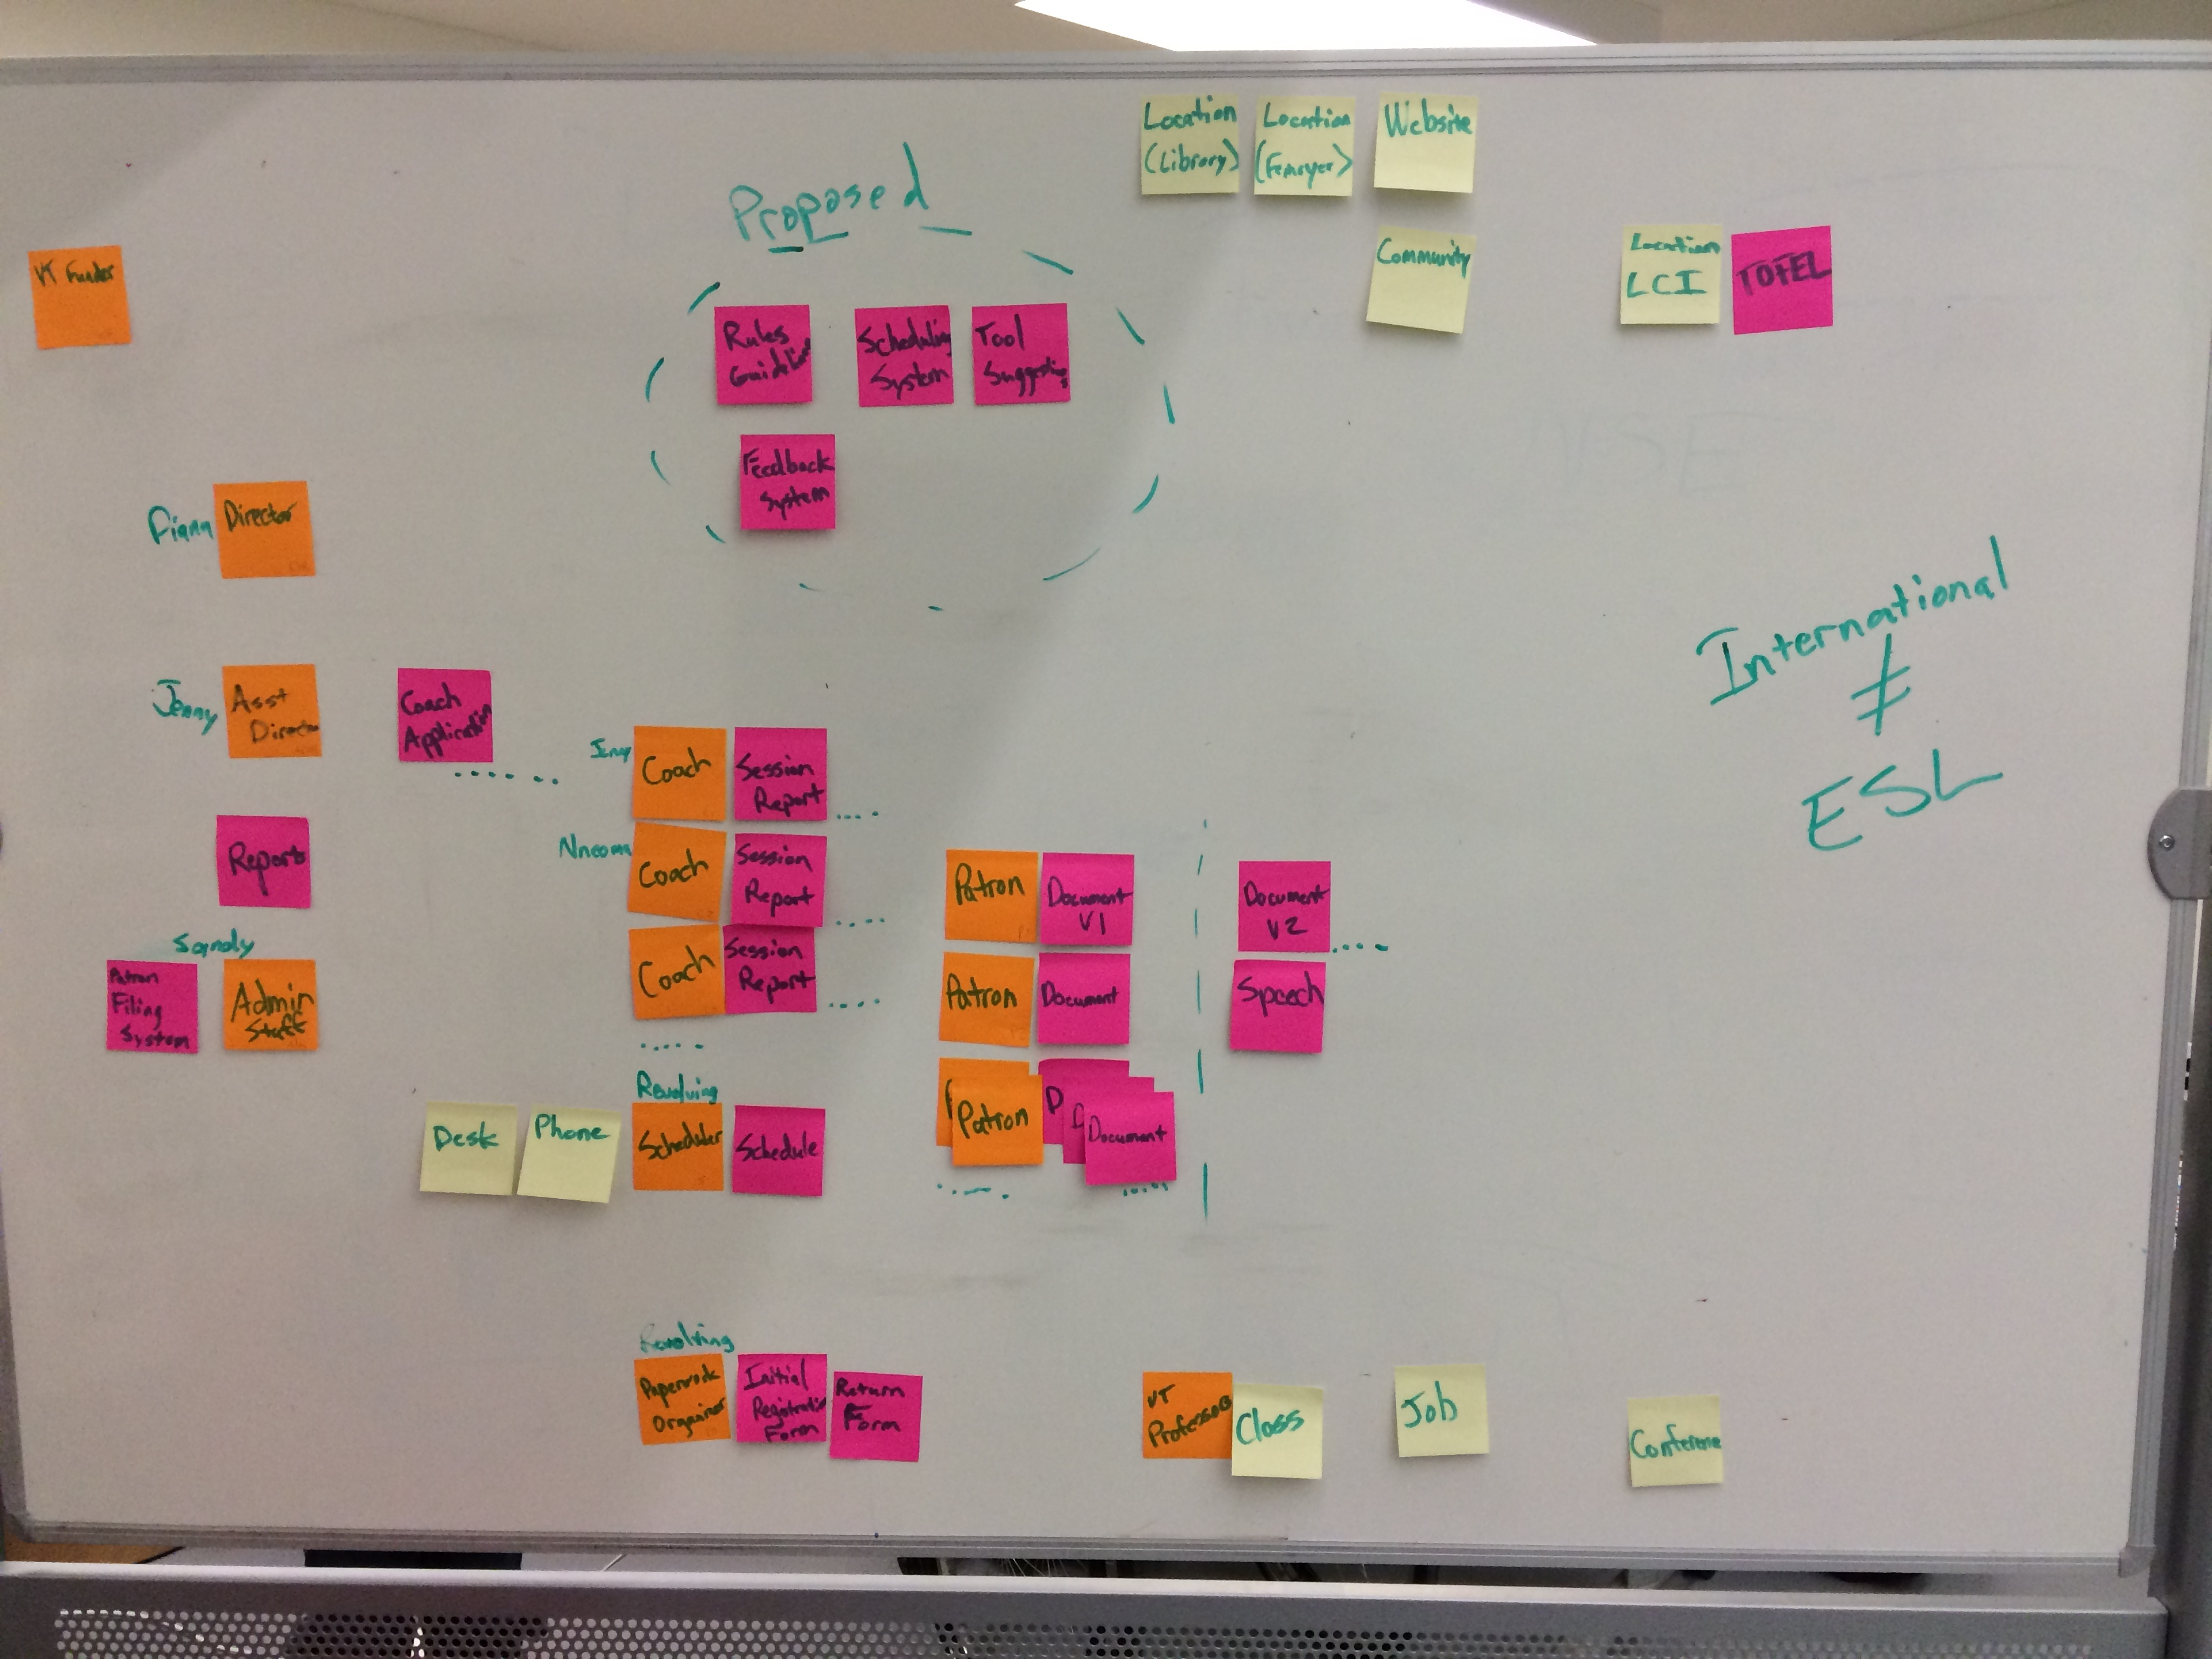
\includegraphics[width=0.95\linewidth]{flow/flowchart_initial}
      \caption{Initial flow chart denoting groupings}
      \label{fig:flowchart_initial}
    \end{subfigure}%
    \begin{subfigure}{.5\linewidth}
      \centering
      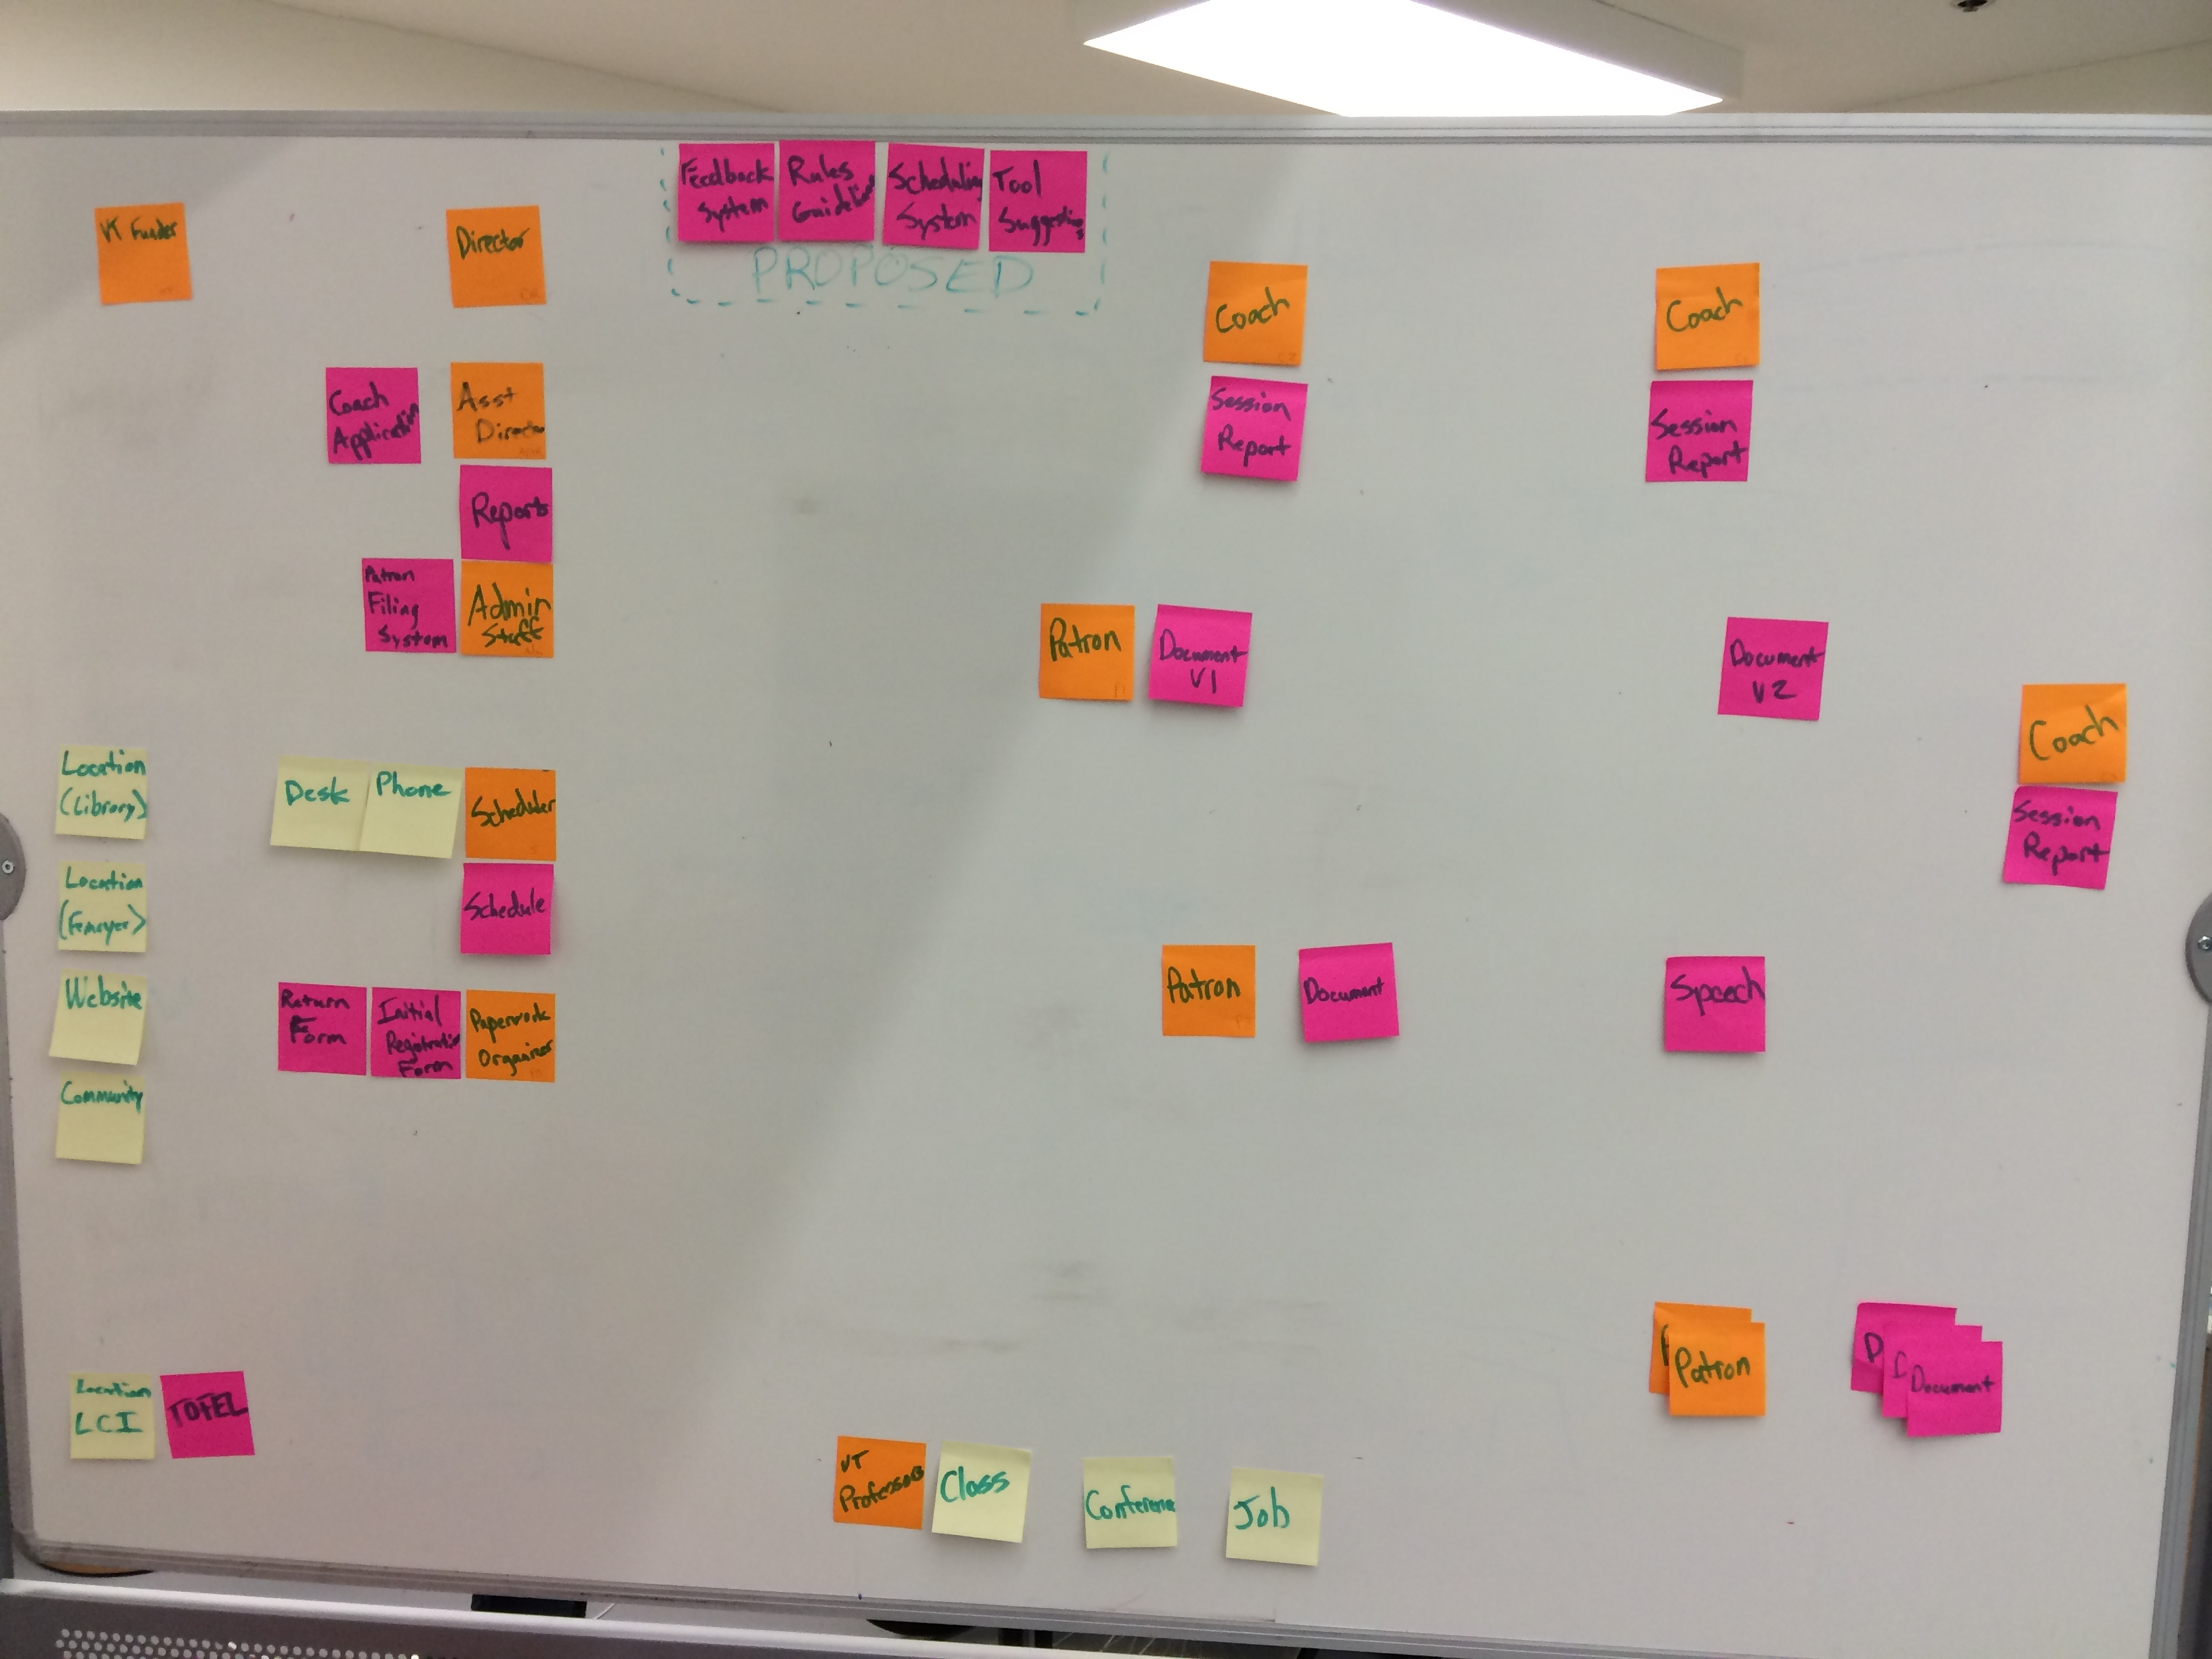
\includegraphics[width=0.95\linewidth]{flow/flowchart_without_arrows}
      \caption{Flow chart in a new grouping}
      \label{fig:flowchart_without_arrows}
    \end{subfigure}\\[1ex]
    \begin{subfigure}{.5\linewidth}
      \centering
      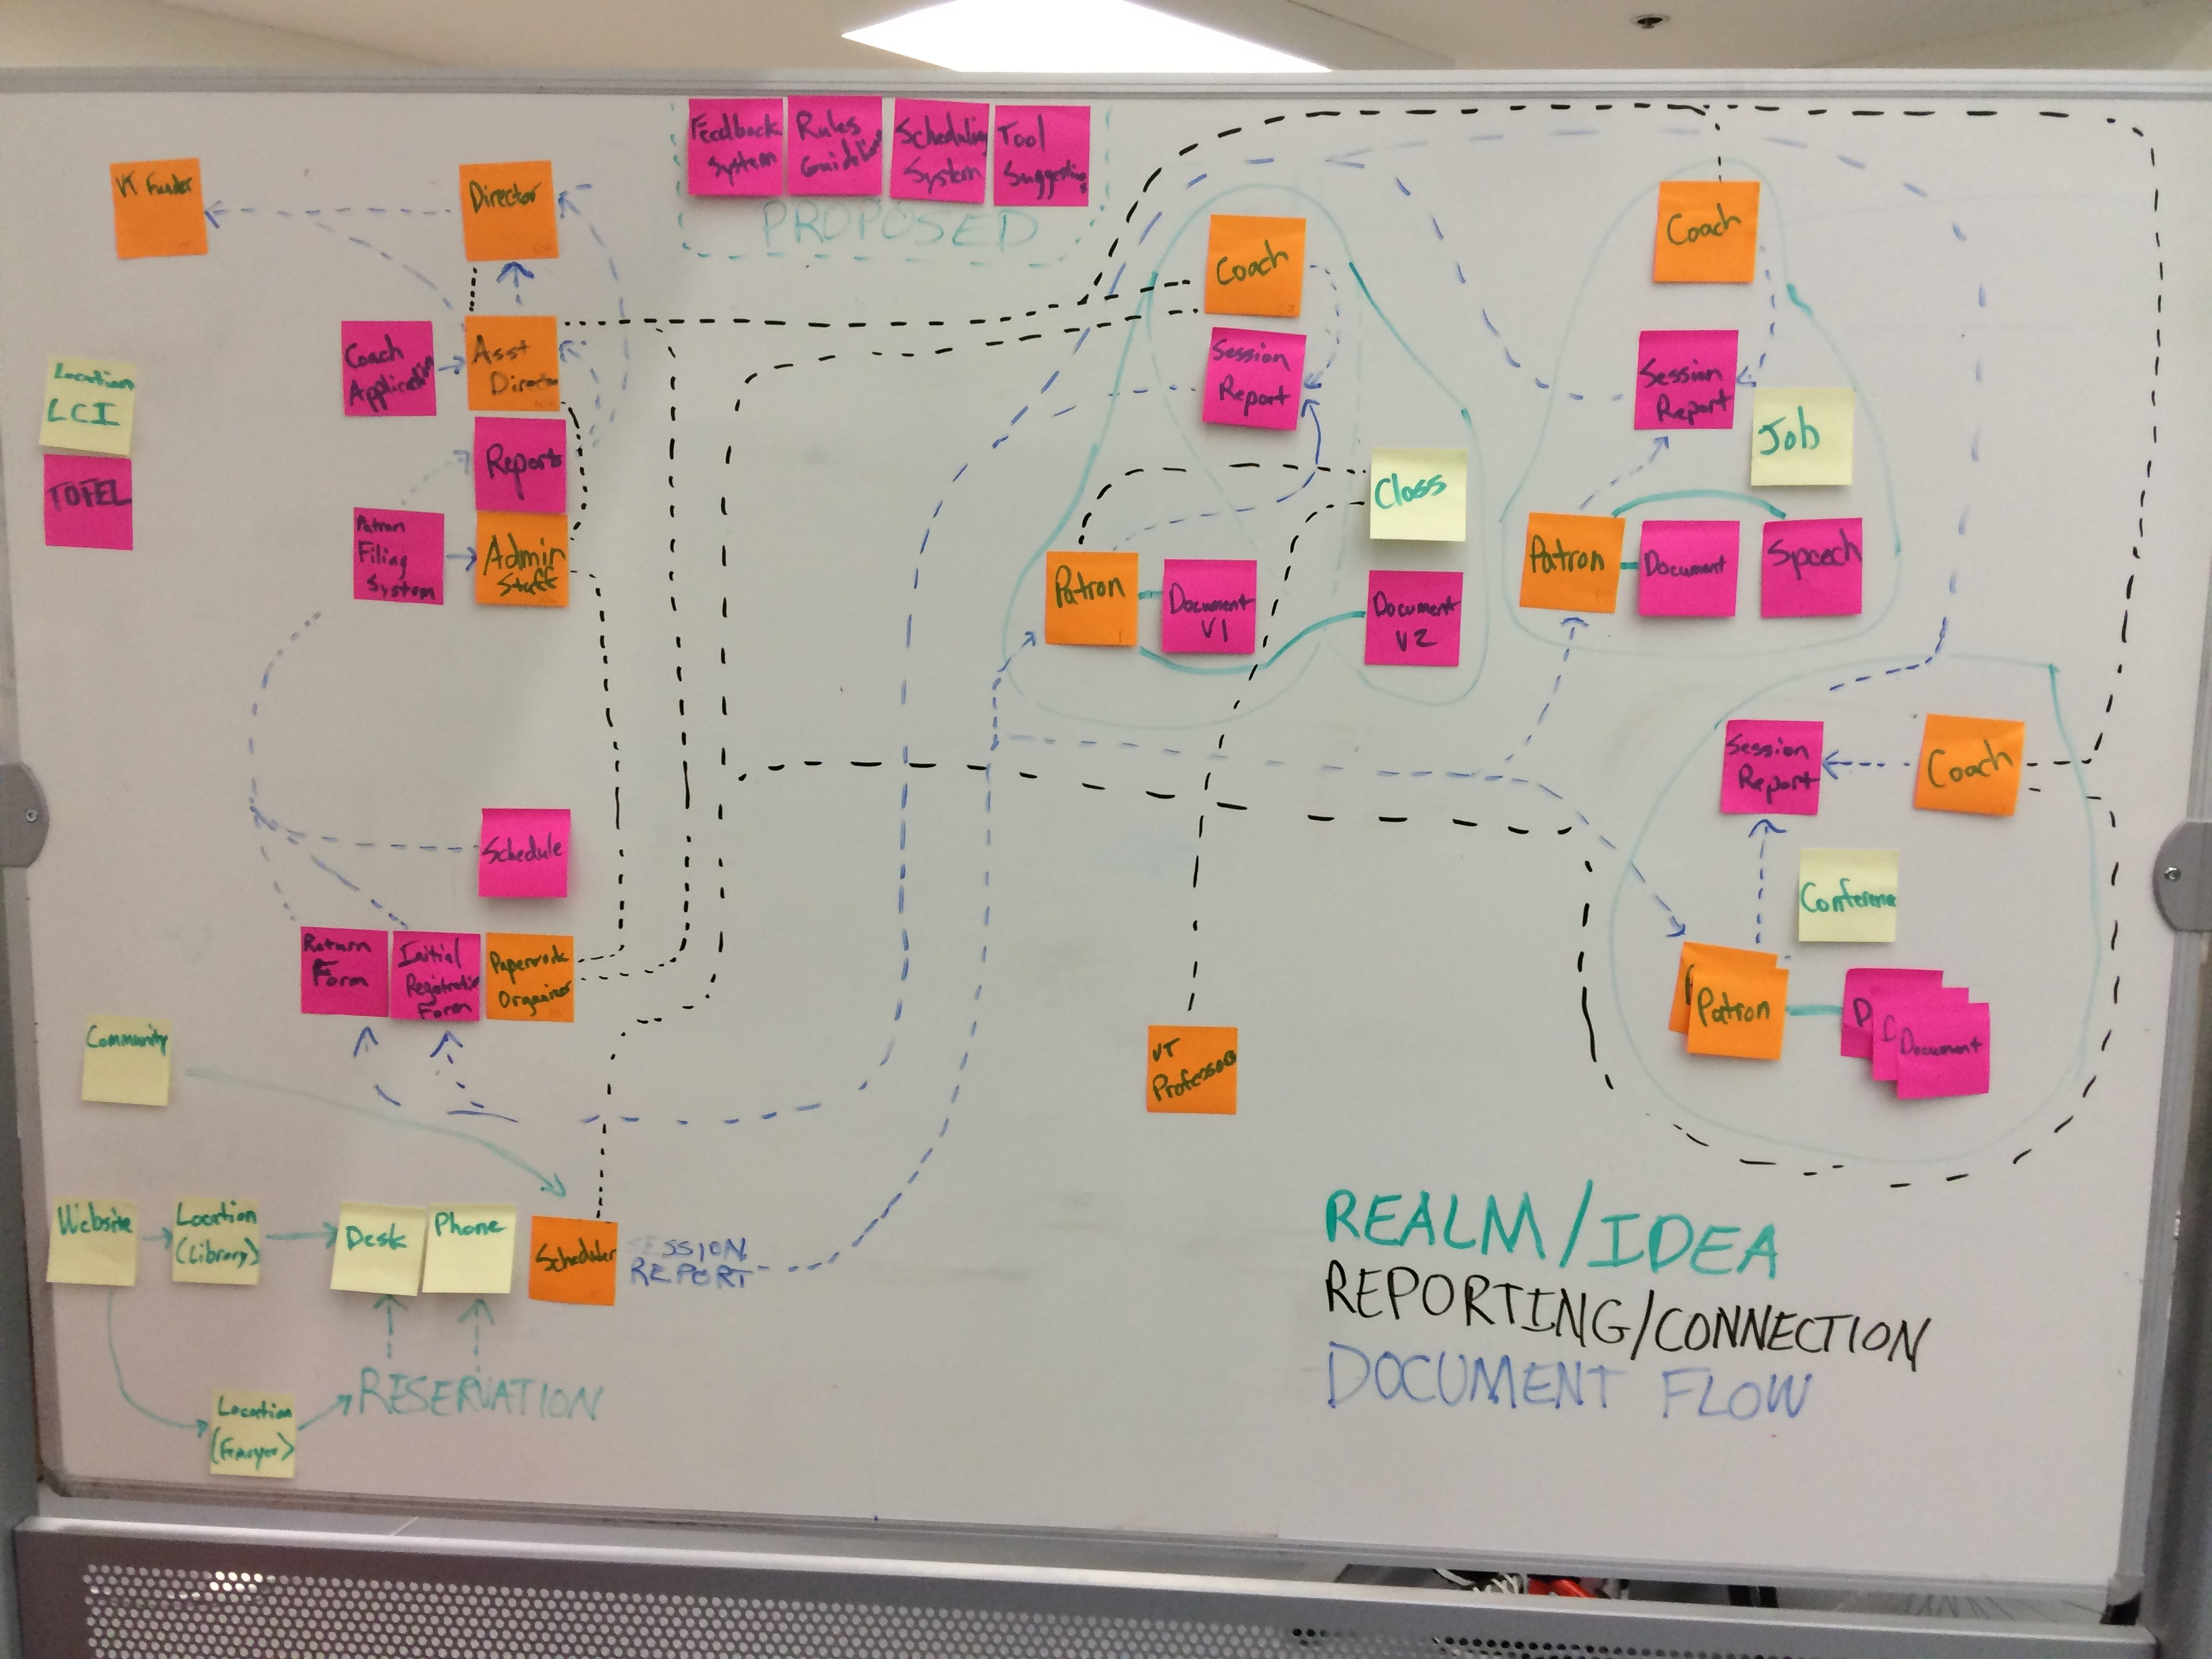
\includegraphics[width=0.95\linewidth]{flow/flowchart_with_arrows}
      \caption{Flow chart with arrows}
      \label{fig:flowchart_with_arrows}
    \end{subfigure}%
    \begin{subfigure}{.5\linewidth}
      \centering
      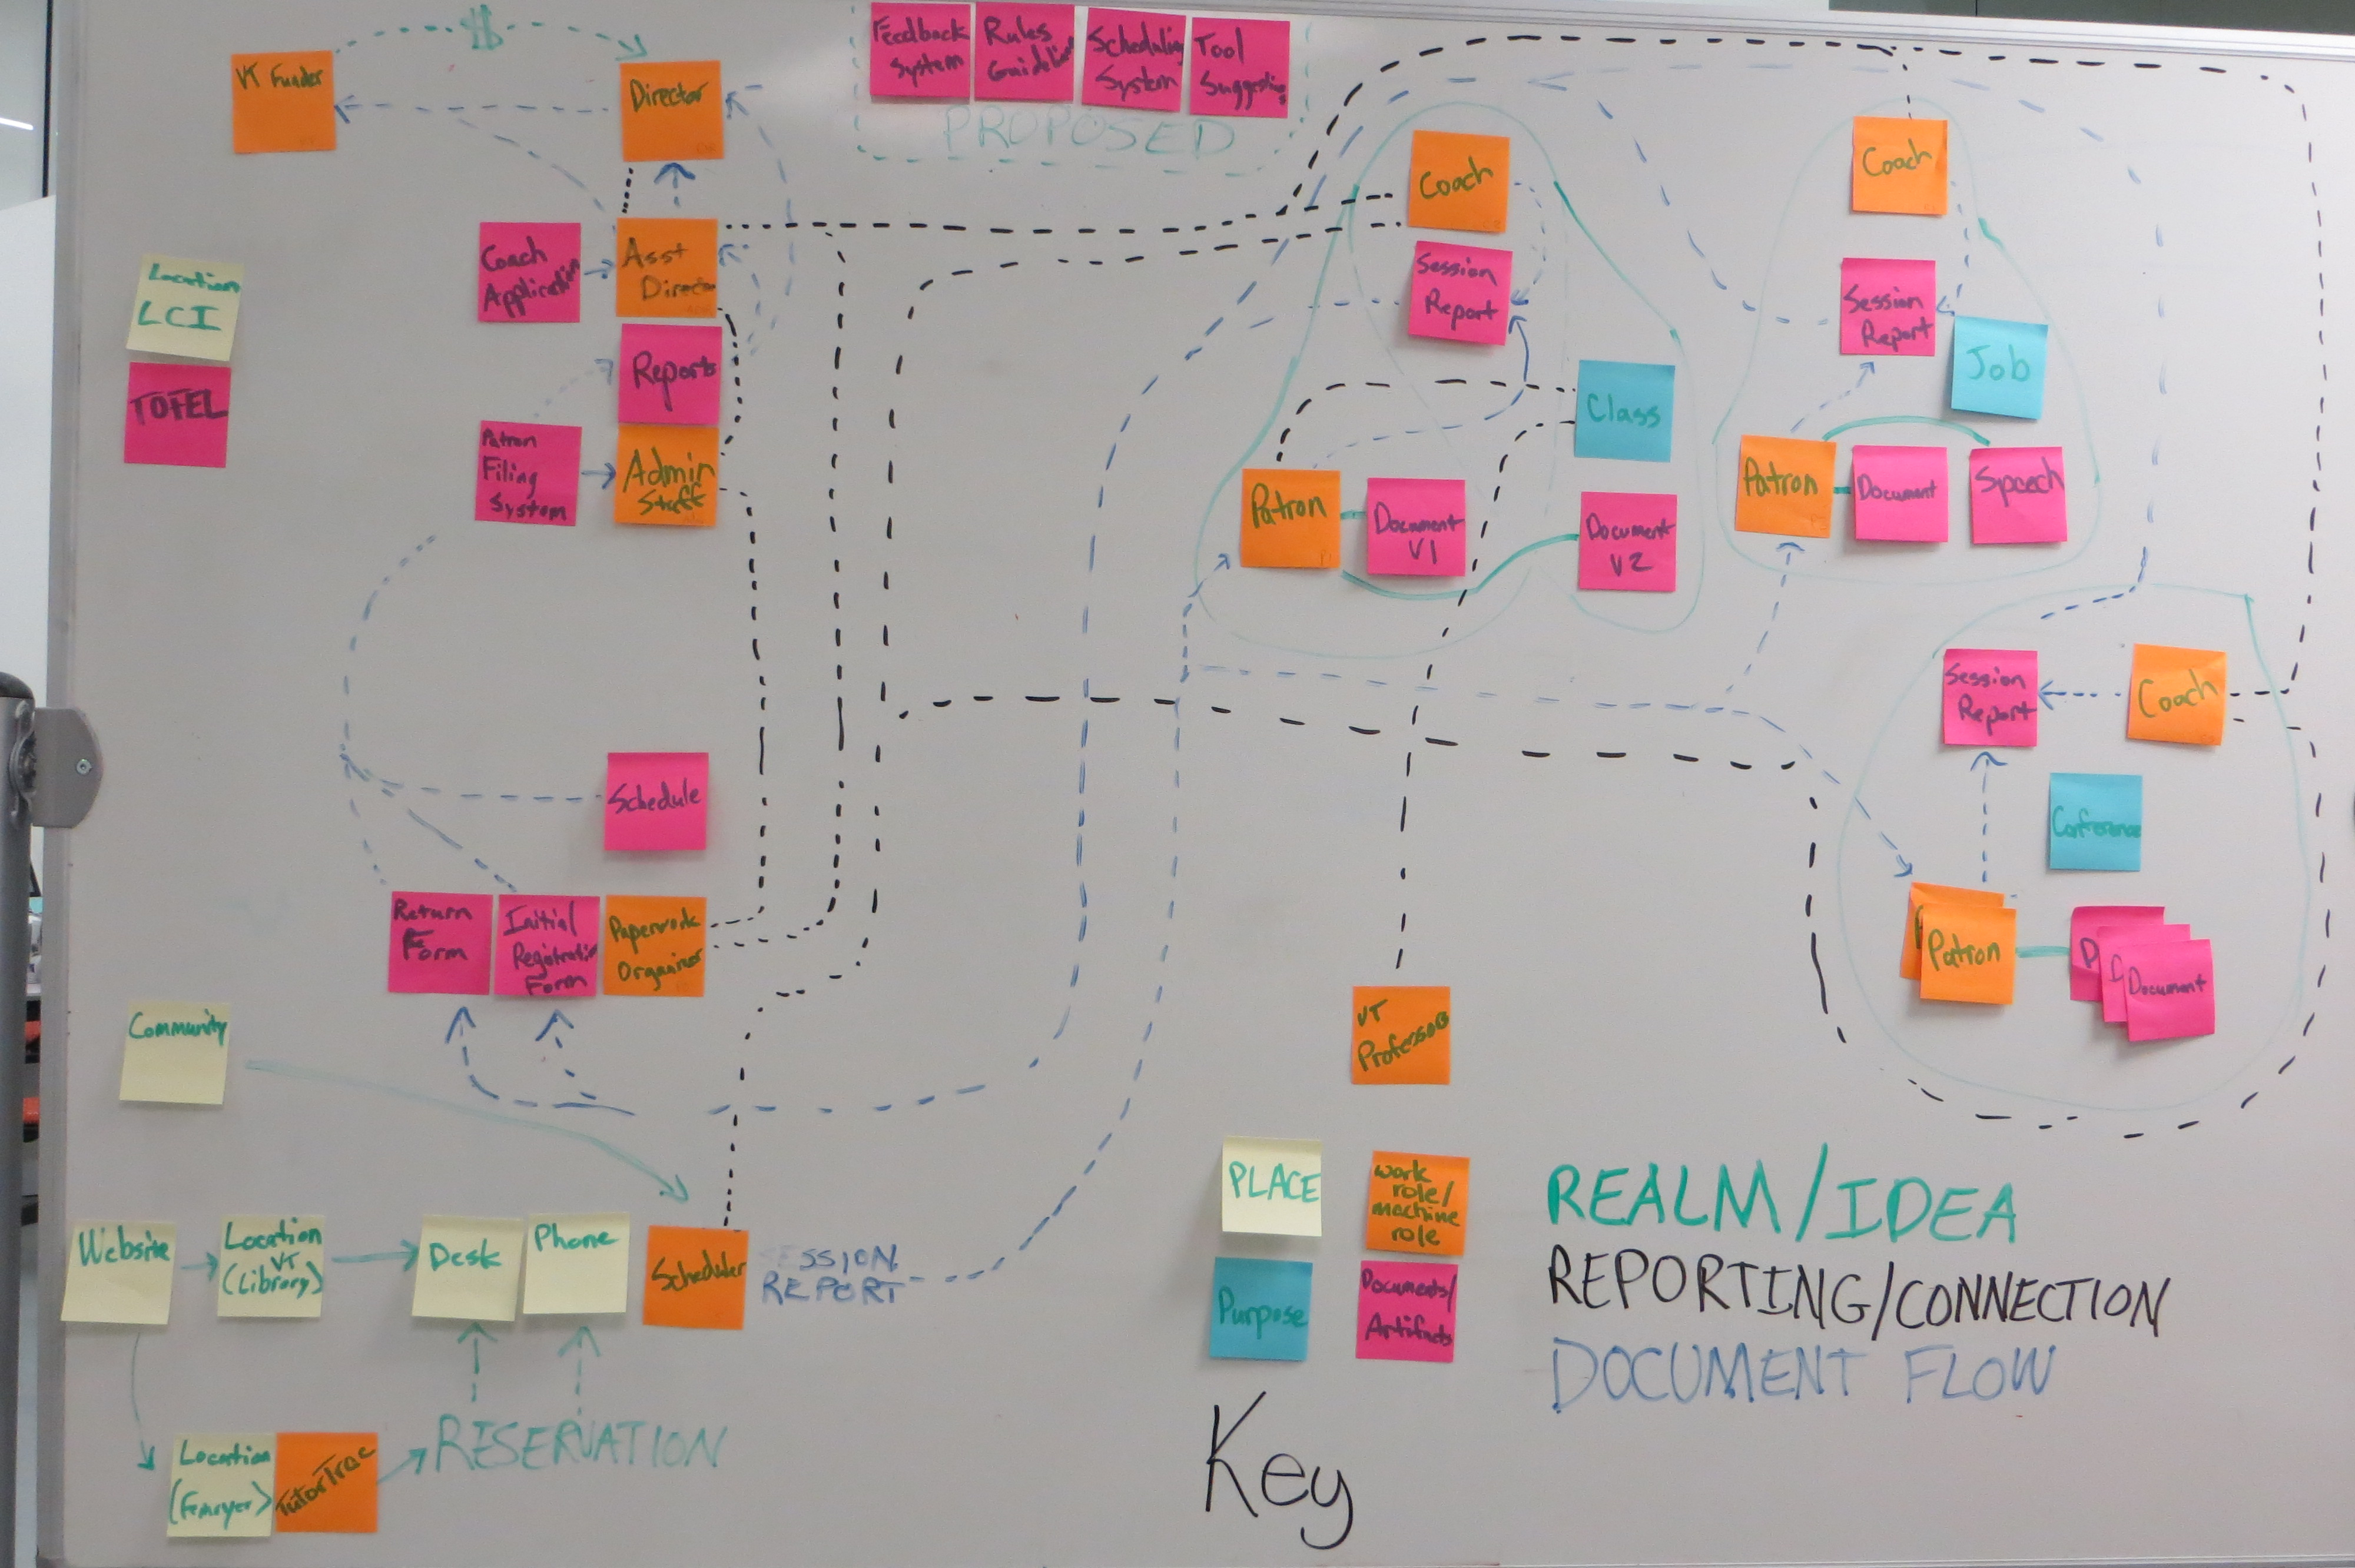
\includegraphics[width=0.95\linewidth]{flow/flowchart_final}
      \caption{The Final Flowchart with Key}
      \label{fig:flowchart_final_small}
    \end{subfigure}
    \caption{Evolution of the Workflow Diagram}
    \label{fig:Workflow_Evolution}
  \end{figure}

\begin{samepage}
\section{Work and Machine Role Nodes} %18
% Show major work roles and machine roles as nodes. 
  Work/machine roles are noted as \textcolor{orange}{orange} squares in the work flow figure of \ref{fig:Workflow_final}.
  Meeting purposes are noted as \textcolor{lightblue}{light blue} squares in the same figure.
  Physical places are marked by \textcolor{beige}{beige} squares.
    \begin{figure}[H]
      \centering
      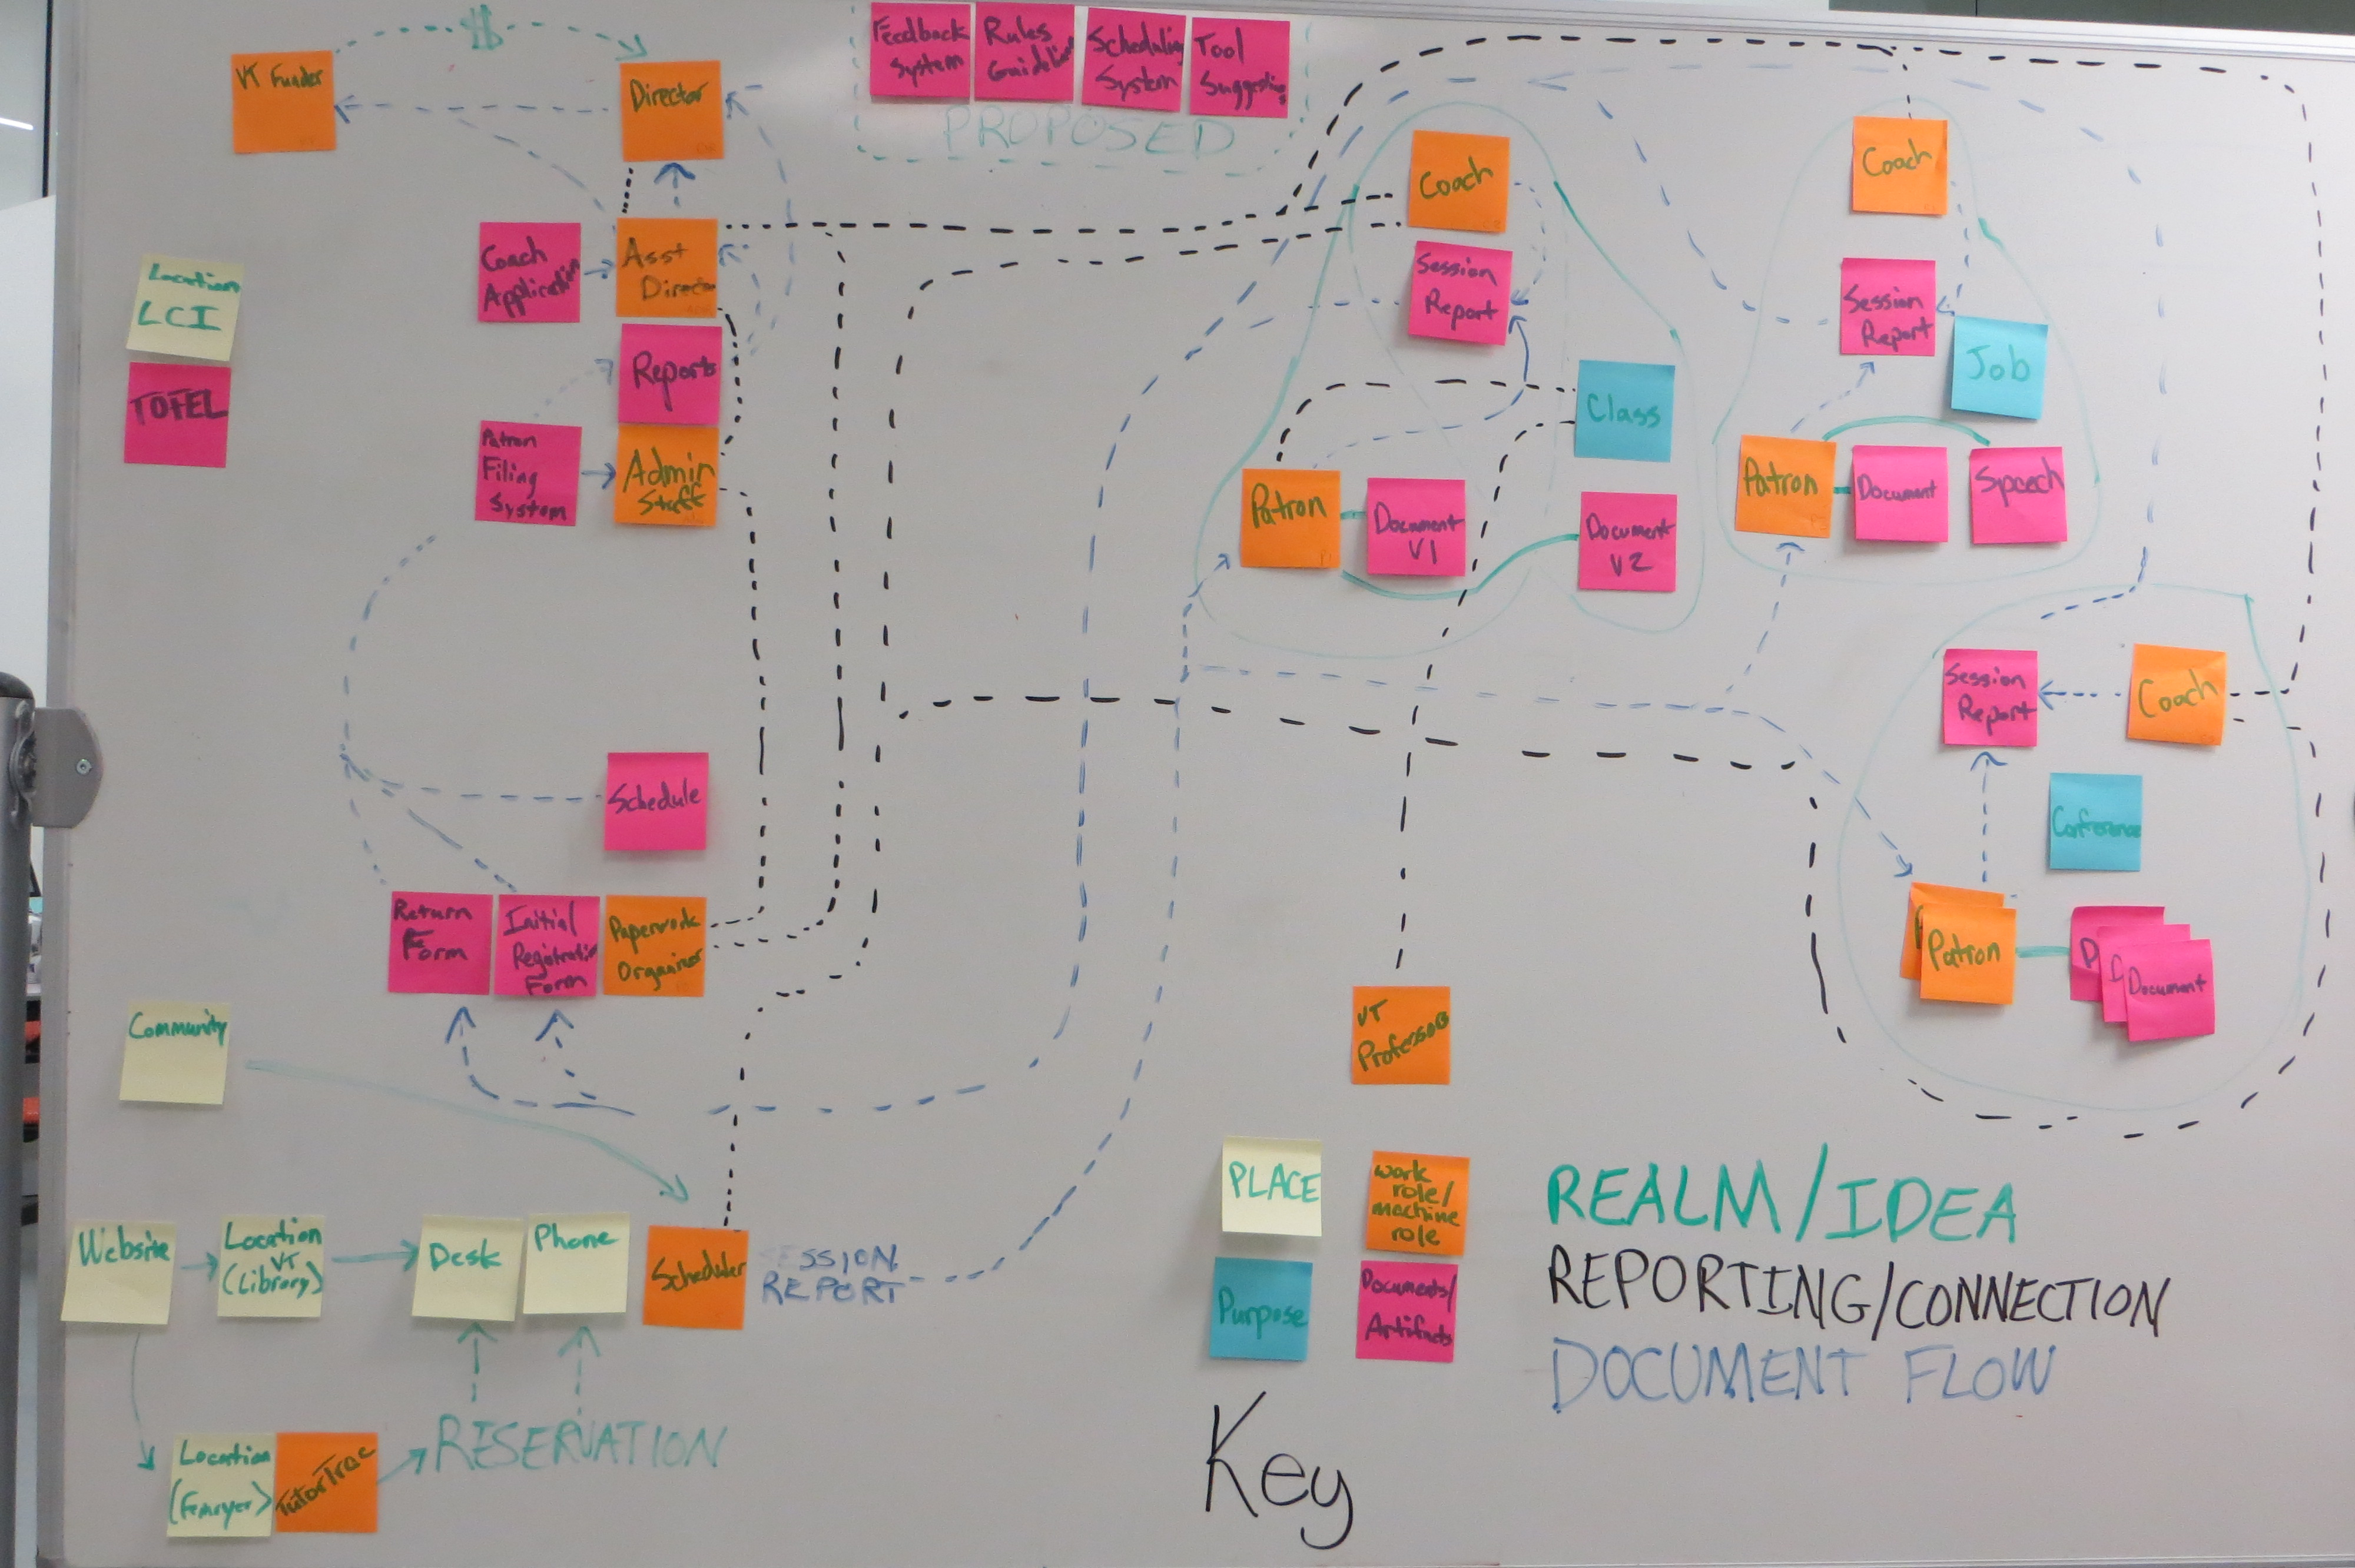
\includegraphics[width=\linewidth]{flow/flowchart_final}
      \caption{The Final Flowchart with Key}
      \label{fig:Workflow_final}
    \end{figure}
  \end{samepage}

\section{Information and Work Flow Arcs} %19
% Show information and work flow as labeled arrows (arcs).
  There are several main ideas covered by the lines and arrows in the Work Flow Diagram [\ref{fig:Workflow_final}].
  The \textcolor{darkgreen}{\textbf{Solid} Green} circles delineate realms for a meeting, and encircle people and artifacts that are used during the process.
  The \textcolor{darkgreen}{D-A-S-H-E-D Green} lines show the linkage or ownership of certain artifacts to their owner.
  The \textcolor{black}{D-A-S-H-E-D Black} lines show who reports to who in the organization.
  The \textcolor{blue}{D-A-S-H-E-D Blue} lines show the flow of information between people and documents.

\section{Outside Information Flow} %20
% Include information flow outside your system (e.g., direct conversations, telephone, etc.) and, where appropriate, label with the channel used (e.g., phone) for each flow. 
  Outside information flow is noted in the corners of the Workflow diagram, namely communication between the directors and funders, and patrons and the reservation system.

\section{Effect of Proposed System} %21
% If helpful, draw a "before" and "after" flow model diagram to show the effect of your proposed system on the work practice (e.g., replace manual information organize now done by office staff and filing cabinets with your system and database).
  We don't have an after, just the proposed systems.  We will continue to incoroparte the proposed ideas into the current workflow diagram and update throughout the project and semester.

\end{document}
